\documentclass{book}
\usepackage[a4paper,top=2.5cm,bottom=2.5cm,left=2.5cm,right=2.5cm]{geometry}
\usepackage{makeidx}
\usepackage{natbib}
\usepackage{graphicx}
\usepackage{multicol}
\usepackage{float}
\usepackage{listings}
\usepackage{color}
\usepackage{ifthen}
\usepackage[table]{xcolor}
\usepackage{textcomp}
\usepackage{alltt}
\usepackage{ifpdf}
\ifpdf
\usepackage[pdftex,
            pagebackref=true,
            colorlinks=true,
            linkcolor=blue,
            unicode
           ]{hyperref}
\else
\usepackage[ps2pdf,
            pagebackref=true,
            colorlinks=true,
            linkcolor=blue,
            unicode
           ]{hyperref}
\usepackage{pspicture}
\fi
\usepackage[utf8]{inputenc}
\usepackage{mathptmx}
\usepackage[scaled=.90]{helvet}
\usepackage{courier}
\usepackage{sectsty}
\usepackage[titles]{tocloft}
\usepackage{doxygen}
\lstset{language=C++,inputencoding=utf8,basicstyle=\footnotesize,breaklines=true,breakatwhitespace=true,tabsize=8,numbers=left }
\makeindex
\setcounter{tocdepth}{3}
\renewcommand{\footrulewidth}{0.4pt}
\renewcommand{\familydefault}{\sfdefault}
\hfuzz=15pt
\setlength{\emergencystretch}{15pt}
\hbadness=750
\tolerance=750
\begin{document}
\hypersetup{pageanchor=false,citecolor=blue}
\begin{titlepage}
\vspace*{7cm}
\begin{center}
{\Large Open Ephys G\-U\-I }\\
\vspace*{1cm}
{\large Generated by Doxygen 1.8.1}\\
\vspace*{0.5cm}
{\small Sun May 20 2012 20:44:18}\\
\end{center}
\end{titlepage}
\clearemptydoublepage
\pagenumbering{roman}
\tableofcontents
\clearemptydoublepage
\pagenumbering{arabic}
\hypersetup{pageanchor=true,citecolor=blue}
\chapter{Class Index}
\section{Class Hierarchy}
This inheritance list is sorted roughly, but not completely, alphabetically\-:\begin{DoxyCompactList}
\item \contentsline{section}{Access\-Class}{\pageref{classAccessClass}}{}
\begin{DoxyCompactList}
\item \contentsline{section}{Audio\-Configuration\-Window}{\pageref{classAudioConfigurationWindow}}{}
\item \contentsline{section}{Audio\-Editor}{\pageref{classAudioEditor}}{}
\item \contentsline{section}{Channel\-Selector}{\pageref{classChannelSelector}}{}
\item \contentsline{section}{Control\-Panel}{\pageref{classControlPanel}}{}
\item \contentsline{section}{Data\-Viewport}{\pageref{classDataViewport}}{}
\item \contentsline{section}{Editor\-Viewport}{\pageref{classEditorViewport}}{}
\item \contentsline{section}{Generic\-Editor}{\pageref{classGenericEditor}}{}
\begin{DoxyCompactList}
\item \contentsline{section}{Event\-Node\-Editor}{\pageref{classEventNodeEditor}}{}
\item \contentsline{section}{Filter\-Editor}{\pageref{classFilterEditor}}{}
\item \contentsline{section}{Merger\-Editor}{\pageref{classMergerEditor}}{}
\item \contentsline{section}{Signal\-Generator\-Editor}{\pageref{classSignalGeneratorEditor}}{}
\item \contentsline{section}{Source\-Node\-Editor}{\pageref{classSourceNodeEditor}}{}
\item \contentsline{section}{Spike\-Detector\-Editor}{\pageref{classSpikeDetectorEditor}}{}
\item \contentsline{section}{Splitter\-Editor}{\pageref{classSplitterEditor}}{}
\item \contentsline{section}{Visualizer\-Editor}{\pageref{classVisualizerEditor}}{}
\begin{DoxyCompactList}
\item \contentsline{section}{Lfp\-Display\-Editor}{\pageref{classLfpDisplayEditor}}{}
\item \contentsline{section}{Spike\-Display\-Editor}{\pageref{classSpikeDisplayEditor}}{}
\end{DoxyCompactList}
\item \contentsline{section}{Wi\-Fi\-Output\-Editor}{\pageref{classWiFiOutputEditor}}{}
\end{DoxyCompactList}
\item \contentsline{section}{Generic\-Processor}{\pageref{classGenericProcessor}}{}
\begin{DoxyCompactList}
\item \contentsline{section}{Audio\-Node}{\pageref{classAudioNode}}{}
\item \contentsline{section}{Event\-Node}{\pageref{classEventNode}}{}
\item \contentsline{section}{Filter\-Node}{\pageref{classFilterNode}}{}
\item \contentsline{section}{Lfp\-Display\-Node}{\pageref{classLfpDisplayNode}}{}
\item \contentsline{section}{Merger}{\pageref{classMerger}}{}
\item \contentsline{section}{Record\-Node}{\pageref{classRecordNode}}{}
\item \contentsline{section}{Resampling\-Node}{\pageref{classResamplingNode}}{}
\item \contentsline{section}{Signal\-Generator}{\pageref{classSignalGenerator}}{}
\item \contentsline{section}{Source\-Node}{\pageref{classSourceNode}}{}
\item \contentsline{section}{Spike\-Detector}{\pageref{classSpikeDetector}}{}
\item \contentsline{section}{Spike\-Display\-Node}{\pageref{classSpikeDisplayNode}}{}
\item \contentsline{section}{Splitter}{\pageref{classSplitter}}{}
\item \contentsline{section}{Wi\-Fi\-Output}{\pageref{classWiFiOutput}}{}
\end{DoxyCompactList}
\item \contentsline{section}{Processor\-Graph}{\pageref{classProcessorGraph}}{}
\item \contentsline{section}{Processor\-List}{\pageref{classProcessorList}}{}
\item \contentsline{section}{Signal\-Chain\-Manager}{\pageref{classSignalChainManager}}{}
\end{DoxyCompactList}
\item \contentsline{section}{Audio\-Component}{\pageref{classAudioComponent}}{}
\item \contentsline{section}{Audio\-Window\-Button}{\pageref{classAudioWindowButton}}{}
\item \contentsline{section}{Base\-U\-I\-Element}{\pageref{classBaseUIElement}}{}
\begin{DoxyCompactList}
\item \contentsline{section}{Electrode\-Plot}{\pageref{classElectrodePlot}}{}
\item \contentsline{section}{Generic\-Axes}{\pageref{classGenericAxes}}{}
\begin{DoxyCompactList}
\item \contentsline{section}{Projection\-Axes}{\pageref{classProjectionAxes}}{}
\item \contentsline{section}{Wave\-Axes}{\pageref{classWaveAxes}}{}
\end{DoxyCompactList}
\item \contentsline{section}{Stereotrode\-Plot}{\pageref{classStereotrodePlot}}{}
\item \contentsline{section}{Tetrode\-Plot}{\pageref{classTetrodePlot}}{}
\end{DoxyCompactList}
\item \contentsline{section}{Record\-Node\-:\-:Channel}{\pageref{structRecordNode_1_1Channel}}{}
\item \contentsline{section}{Channel\-Selector\-Button}{\pageref{classChannelSelectorButton}}{}
\item \contentsline{section}{Clock}{\pageref{classClock}}{}
\item \contentsline{section}{Control\-Panel\-Button}{\pageref{classControlPanelButton}}{}
\item \contentsline{section}{C\-P\-U\-Meter}{\pageref{classCPUMeter}}{}
\item \contentsline{section}{Custom\-Look\-And\-Feel}{\pageref{classCustomLookAndFeel}}{}
\item \contentsline{section}{Data\-Buffer}{\pageref{classDataBuffer}}{}
\item \contentsline{section}{Data\-Thread}{\pageref{classDataThread}}{}
\begin{DoxyCompactList}
\item \contentsline{section}{File\-Reader\-Thread}{\pageref{classFileReaderThread}}{}
\item \contentsline{section}{F\-P\-G\-A\-Thread}{\pageref{classFPGAThread}}{}
\item \contentsline{section}{Intan\-Thread}{\pageref{classIntanThread}}{}
\item \contentsline{section}{Network\-Thread}{\pageref{classNetworkThread}}{}
\end{DoxyCompactList}
\item \contentsline{section}{Data\-Window}{\pageref{classDataWindow}}{}
\item \contentsline{section}{Disk\-Space\-Meter}{\pageref{classDiskSpaceMeter}}{}
\item \contentsline{section}{Drawer\-Button}{\pageref{classDrawerButton}}{}
\item \contentsline{section}{Editor\-Button}{\pageref{classEditorButton}}{}
\item \contentsline{section}{Editor\-Scroll\-Button}{\pageref{classEditorScrollButton}}{}
\item \contentsline{section}{Editor\-Viewport\-Button}{\pageref{classEditorViewportButton}}{}
\item \contentsline{section}{Spike\-Detector\-:\-:Electrode}{\pageref{structSpikeDetector_1_1Electrode}}{}
\item \contentsline{section}{Electrode\-Button}{\pageref{classElectrodeButton}}{}
\item \contentsline{section}{Electrode\-Editor\-Button}{\pageref{classElectrodeEditorButton}}{}
\item \contentsline{section}{Image\-Icon}{\pageref{classImageIcon}}{}
\item \contentsline{section}{Lfp\-Viewer}{\pageref{classLfpViewer}}{}
\item \contentsline{section}{Main\-Window}{\pageref{classMainWindow}}{}
\item \contentsline{section}{Message\-Center}{\pageref{classMessageCenter}}{}
\item \contentsline{section}{Mute\-Button}{\pageref{classMuteButton}}{}
\item \contentsline{section}{Open\-G\-L\-Canvas}{\pageref{classOpenGLCanvas}}{}
\begin{DoxyCompactList}
\item \contentsline{section}{Info\-Label}{\pageref{classInfoLabel}}{}
\item \contentsline{section}{Processor\-List}{\pageref{classProcessorList}}{}
\item \contentsline{section}{Visualizer}{\pageref{classVisualizer}}{}
\begin{DoxyCompactList}
\item \contentsline{section}{Lfp\-Display\-Canvas}{\pageref{classLfpDisplayCanvas}}{}
\item \contentsline{section}{Spike\-Display\-Canvas}{\pageref{classSpikeDisplayCanvas}}{}
\end{DoxyCompactList}
\end{DoxyCompactList}
\item \contentsline{section}{Parameter}{\pageref{classParameter}}{}
\item \contentsline{section}{Parameter\-Button}{\pageref{classParameterButton}}{}
\item \contentsline{section}{Parameter\-Checkbox}{\pageref{classParameterCheckbox}}{}
\item \contentsline{section}{Parameter\-Editor}{\pageref{classParameterEditor}}{}
\item \contentsline{section}{Parameter\-Slider}{\pageref{classParameterSlider}}{}
\item \contentsline{section}{Play\-Button}{\pageref{classPlayButton}}{}
\item \contentsline{section}{Processor\-List\-Item}{\pageref{classProcessorListItem}}{}
\item \contentsline{section}{Generic\-Processor\-:\-:Processor\-Settings}{\pageref{structGenericProcessor_1_1ProcessorSettings}}{}
\item \contentsline{section}{Record\-Button}{\pageref{classRecordButton}}{}
\item \contentsline{section}{Selector\-Button}{\pageref{classSelectorButton}}{}
\item \contentsline{section}{Signal\-Chain\-Scroll\-Button}{\pageref{classSignalChainScrollButton}}{}
\item \contentsline{section}{Signal\-Chain\-Tab\-Button}{\pageref{classSignalChainTabButton}}{}
\item \contentsline{section}{Simple\-Key\-Event}{\pageref{structSimpleKeyEvent}}{}
\item \contentsline{section}{Spike\-Object}{\pageref{structSpikeObject}}{}
\item \contentsline{section}{Threshold\-Slider}{\pageref{classThresholdSlider}}{}
\item \contentsline{section}{Triangle\-Button}{\pageref{classTriangleButton}}{}
\item \contentsline{section}{U\-I\-Component}{\pageref{classUIComponent}}{}
\item \contentsline{section}{Utility\-Button}{\pageref{classUtilityButton}}{}
\item \contentsline{section}{Waveform\-Selector}{\pageref{classWaveformSelector}}{}
\end{DoxyCompactList}

\chapter{Class Index}
\section{Class List}
Here are the classes, structs, unions and interfaces with brief descriptions\-:\begin{DoxyCompactList}
\item\contentsline{section}{\hyperlink{classAccessClass}{Access\-Class} }{\pageref{classAccessClass}}{}
\item\contentsline{section}{\hyperlink{classAudioComponent}{Audio\-Component} }{\pageref{classAudioComponent}}{}
\item\contentsline{section}{\hyperlink{classAudioConfigurationWindow}{Audio\-Configuration\-Window} }{\pageref{classAudioConfigurationWindow}}{}
\item\contentsline{section}{\hyperlink{classAudioEditor}{Audio\-Editor} }{\pageref{classAudioEditor}}{}
\item\contentsline{section}{\hyperlink{classAudioNode}{Audio\-Node} }{\pageref{classAudioNode}}{}
\item\contentsline{section}{\hyperlink{classAudioWindowButton}{Audio\-Window\-Button} }{\pageref{classAudioWindowButton}}{}
\item\contentsline{section}{\hyperlink{classBaseUIElement}{Base\-U\-I\-Element} }{\pageref{classBaseUIElement}}{}
\item\contentsline{section}{\hyperlink{structRecordNode_1_1Channel}{Record\-Node\-::\-Channel} }{\pageref{structRecordNode_1_1Channel}}{}
\item\contentsline{section}{\hyperlink{classChannelSelector}{Channel\-Selector} }{\pageref{classChannelSelector}}{}
\item\contentsline{section}{\hyperlink{classChannelSelectorButton}{Channel\-Selector\-Button} }{\pageref{classChannelSelectorButton}}{}
\item\contentsline{section}{\hyperlink{classClock}{Clock} }{\pageref{classClock}}{}
\item\contentsline{section}{\hyperlink{classControlPanel}{Control\-Panel} }{\pageref{classControlPanel}}{}
\item\contentsline{section}{\hyperlink{classControlPanelButton}{Control\-Panel\-Button} }{\pageref{classControlPanelButton}}{}
\item\contentsline{section}{\hyperlink{classCPUMeter}{C\-P\-U\-Meter} }{\pageref{classCPUMeter}}{}
\item\contentsline{section}{\hyperlink{classCustomLookAndFeel}{Custom\-Look\-And\-Feel} }{\pageref{classCustomLookAndFeel}}{}
\item\contentsline{section}{\hyperlink{classDataBuffer}{Data\-Buffer} }{\pageref{classDataBuffer}}{}
\item\contentsline{section}{\hyperlink{classDataThread}{Data\-Thread} }{\pageref{classDataThread}}{}
\item\contentsline{section}{\hyperlink{classDataViewport}{Data\-Viewport} }{\pageref{classDataViewport}}{}
\item\contentsline{section}{\hyperlink{classDataWindow}{Data\-Window} }{\pageref{classDataWindow}}{}
\item\contentsline{section}{\hyperlink{classDiskSpaceMeter}{Disk\-Space\-Meter} }{\pageref{classDiskSpaceMeter}}{}
\item\contentsline{section}{\hyperlink{classDrawerButton}{Drawer\-Button} }{\pageref{classDrawerButton}}{}
\item\contentsline{section}{\hyperlink{classEditorButton}{Editor\-Button} }{\pageref{classEditorButton}}{}
\item\contentsline{section}{\hyperlink{classEditorScrollButton}{Editor\-Scroll\-Button} }{\pageref{classEditorScrollButton}}{}
\item\contentsline{section}{\hyperlink{classEditorViewport}{Editor\-Viewport} }{\pageref{classEditorViewport}}{}
\item\contentsline{section}{\hyperlink{classEditorViewportButton}{Editor\-Viewport\-Button} }{\pageref{classEditorViewportButton}}{}
\item\contentsline{section}{\hyperlink{structSpikeDetector_1_1Electrode}{Spike\-Detector\-::\-Electrode} }{\pageref{structSpikeDetector_1_1Electrode}}{}
\item\contentsline{section}{\hyperlink{classElectrodeButton}{Electrode\-Button} }{\pageref{classElectrodeButton}}{}
\item\contentsline{section}{\hyperlink{classElectrodeEditorButton}{Electrode\-Editor\-Button} }{\pageref{classElectrodeEditorButton}}{}
\item\contentsline{section}{\hyperlink{classElectrodePlot}{Electrode\-Plot} }{\pageref{classElectrodePlot}}{}
\item\contentsline{section}{\hyperlink{classEventNode}{Event\-Node} }{\pageref{classEventNode}}{}
\item\contentsline{section}{\hyperlink{classEventNodeEditor}{Event\-Node\-Editor} }{\pageref{classEventNodeEditor}}{}
\item\contentsline{section}{\hyperlink{classFileReaderThread}{File\-Reader\-Thread} }{\pageref{classFileReaderThread}}{}
\item\contentsline{section}{\hyperlink{classFilterEditor}{Filter\-Editor} }{\pageref{classFilterEditor}}{}
\item\contentsline{section}{\hyperlink{classFilterNode}{Filter\-Node} }{\pageref{classFilterNode}}{}
\item\contentsline{section}{\hyperlink{classFPGAThread}{F\-P\-G\-A\-Thread} }{\pageref{classFPGAThread}}{}
\item\contentsline{section}{\hyperlink{classGenericAxes}{Generic\-Axes} }{\pageref{classGenericAxes}}{}
\item\contentsline{section}{\hyperlink{classGenericEditor}{Generic\-Editor} }{\pageref{classGenericEditor}}{}
\item\contentsline{section}{\hyperlink{classGenericProcessor}{Generic\-Processor} }{\pageref{classGenericProcessor}}{}
\item\contentsline{section}{\hyperlink{classImageIcon}{Image\-Icon} }{\pageref{classImageIcon}}{}
\item\contentsline{section}{\hyperlink{classInfoLabel}{Info\-Label} }{\pageref{classInfoLabel}}{}
\item\contentsline{section}{\hyperlink{classIntanThread}{Intan\-Thread} }{\pageref{classIntanThread}}{}
\item\contentsline{section}{\hyperlink{classLfpDisplayCanvas}{Lfp\-Display\-Canvas} }{\pageref{classLfpDisplayCanvas}}{}
\item\contentsline{section}{\hyperlink{classLfpDisplayEditor}{Lfp\-Display\-Editor} }{\pageref{classLfpDisplayEditor}}{}
\item\contentsline{section}{\hyperlink{classLfpDisplayNode}{Lfp\-Display\-Node} }{\pageref{classLfpDisplayNode}}{}
\item\contentsline{section}{\hyperlink{classLfpViewer}{Lfp\-Viewer} }{\pageref{classLfpViewer}}{}
\item\contentsline{section}{\hyperlink{classMainWindow}{Main\-Window} }{\pageref{classMainWindow}}{}
\item\contentsline{section}{\hyperlink{classMerger}{Merger} }{\pageref{classMerger}}{}
\item\contentsline{section}{\hyperlink{classMergerEditor}{Merger\-Editor} }{\pageref{classMergerEditor}}{}
\item\contentsline{section}{\hyperlink{classMessageCenter}{Message\-Center} }{\pageref{classMessageCenter}}{}
\item\contentsline{section}{\hyperlink{classMuteButton}{Mute\-Button} }{\pageref{classMuteButton}}{}
\item\contentsline{section}{\hyperlink{classNetworkThread}{Network\-Thread} }{\pageref{classNetworkThread}}{}
\item\contentsline{section}{\hyperlink{classOpenGLCanvas}{Open\-G\-L\-Canvas} }{\pageref{classOpenGLCanvas}}{}
\item\contentsline{section}{\hyperlink{classParameter}{Parameter} }{\pageref{classParameter}}{}
\item\contentsline{section}{\hyperlink{classParameterButton}{Parameter\-Button} }{\pageref{classParameterButton}}{}
\item\contentsline{section}{\hyperlink{classParameterCheckbox}{Parameter\-Checkbox} }{\pageref{classParameterCheckbox}}{}
\item\contentsline{section}{\hyperlink{classParameterEditor}{Parameter\-Editor} }{\pageref{classParameterEditor}}{}
\item\contentsline{section}{\hyperlink{classParameterSlider}{Parameter\-Slider} }{\pageref{classParameterSlider}}{}
\item\contentsline{section}{\hyperlink{classPlayButton}{Play\-Button} }{\pageref{classPlayButton}}{}
\item\contentsline{section}{\hyperlink{classProcessorGraph}{Processor\-Graph} }{\pageref{classProcessorGraph}}{}
\item\contentsline{section}{\hyperlink{classProcessorList}{Processor\-List} }{\pageref{classProcessorList}}{}
\item\contentsline{section}{\hyperlink{classProcessorListItem}{Processor\-List\-Item} }{\pageref{classProcessorListItem}}{}
\item\contentsline{section}{\hyperlink{structGenericProcessor_1_1ProcessorSettings}{Generic\-Processor\-::\-Processor\-Settings} }{\pageref{structGenericProcessor_1_1ProcessorSettings}}{}
\item\contentsline{section}{\hyperlink{classProjectionAxes}{Projection\-Axes} }{\pageref{classProjectionAxes}}{}
\item\contentsline{section}{\hyperlink{classRecordButton}{Record\-Button} }{\pageref{classRecordButton}}{}
\item\contentsline{section}{\hyperlink{classRecordNode}{Record\-Node} }{\pageref{classRecordNode}}{}
\item\contentsline{section}{\hyperlink{classResamplingNode}{Resampling\-Node} }{\pageref{classResamplingNode}}{}
\item\contentsline{section}{\hyperlink{classSelectorButton}{Selector\-Button} }{\pageref{classSelectorButton}}{}
\item\contentsline{section}{\hyperlink{classSignalChainManager}{Signal\-Chain\-Manager} }{\pageref{classSignalChainManager}}{}
\item\contentsline{section}{\hyperlink{classSignalChainScrollButton}{Signal\-Chain\-Scroll\-Button} }{\pageref{classSignalChainScrollButton}}{}
\item\contentsline{section}{\hyperlink{classSignalChainTabButton}{Signal\-Chain\-Tab\-Button} }{\pageref{classSignalChainTabButton}}{}
\item\contentsline{section}{\hyperlink{classSignalGenerator}{Signal\-Generator} }{\pageref{classSignalGenerator}}{}
\item\contentsline{section}{\hyperlink{classSignalGeneratorEditor}{Signal\-Generator\-Editor} }{\pageref{classSignalGeneratorEditor}}{}
\item\contentsline{section}{\hyperlink{structSimpleKeyEvent}{Simple\-Key\-Event} }{\pageref{structSimpleKeyEvent}}{}
\item\contentsline{section}{\hyperlink{classSourceNode}{Source\-Node} }{\pageref{classSourceNode}}{}
\item\contentsline{section}{\hyperlink{classSourceNodeEditor}{Source\-Node\-Editor} }{\pageref{classSourceNodeEditor}}{}
\item\contentsline{section}{\hyperlink{classSpikeDetector}{Spike\-Detector} }{\pageref{classSpikeDetector}}{}
\item\contentsline{section}{\hyperlink{classSpikeDetectorEditor}{Spike\-Detector\-Editor} }{\pageref{classSpikeDetectorEditor}}{}
\item\contentsline{section}{\hyperlink{classSpikeDisplayCanvas}{Spike\-Display\-Canvas} }{\pageref{classSpikeDisplayCanvas}}{}
\item\contentsline{section}{\hyperlink{classSpikeDisplayEditor}{Spike\-Display\-Editor} }{\pageref{classSpikeDisplayEditor}}{}
\item\contentsline{section}{\hyperlink{classSpikeDisplayNode}{Spike\-Display\-Node} }{\pageref{classSpikeDisplayNode}}{}
\item\contentsline{section}{\hyperlink{structSpikeObject}{Spike\-Object} }{\pageref{structSpikeObject}}{}
\item\contentsline{section}{\hyperlink{classSplitter}{Splitter} }{\pageref{classSplitter}}{}
\item\contentsline{section}{\hyperlink{classSplitterEditor}{Splitter\-Editor} }{\pageref{classSplitterEditor}}{}
\item\contentsline{section}{\hyperlink{classStereotrodePlot}{Stereotrode\-Plot} }{\pageref{classStereotrodePlot}}{}
\item\contentsline{section}{\hyperlink{classTetrodePlot}{Tetrode\-Plot} }{\pageref{classTetrodePlot}}{}
\item\contentsline{section}{\hyperlink{classThresholdSlider}{Threshold\-Slider} }{\pageref{classThresholdSlider}}{}
\item\contentsline{section}{\hyperlink{classTriangleButton}{Triangle\-Button} }{\pageref{classTriangleButton}}{}
\item\contentsline{section}{\hyperlink{classUIComponent}{U\-I\-Component} }{\pageref{classUIComponent}}{}
\item\contentsline{section}{\hyperlink{classUtilityButton}{Utility\-Button} }{\pageref{classUtilityButton}}{}
\item\contentsline{section}{\hyperlink{classVisualizer}{Visualizer} }{\pageref{classVisualizer}}{}
\item\contentsline{section}{\hyperlink{classVisualizerEditor}{Visualizer\-Editor} }{\pageref{classVisualizerEditor}}{}
\item\contentsline{section}{\hyperlink{classWaveAxes}{Wave\-Axes} }{\pageref{classWaveAxes}}{}
\item\contentsline{section}{\hyperlink{classWaveformSelector}{Waveform\-Selector} }{\pageref{classWaveformSelector}}{}
\item\contentsline{section}{\hyperlink{classWiFiOutput}{Wi\-Fi\-Output} }{\pageref{classWiFiOutput}}{}
\item\contentsline{section}{\hyperlink{classWiFiOutputEditor}{Wi\-Fi\-Output\-Editor} }{\pageref{classWiFiOutputEditor}}{}
\end{DoxyCompactList}

\chapter{Class Documentation}
\hypertarget{classAccessClass}{\section{Access\-Class Class Reference}
\label{classAccessClass}\index{Access\-Class@{Access\-Class}}
}


{\ttfamily \#include $<$Access\-Class.\-h$>$}

Inheritance diagram for Access\-Class\-:\begin{figure}[H]
\begin{center}
\leavevmode
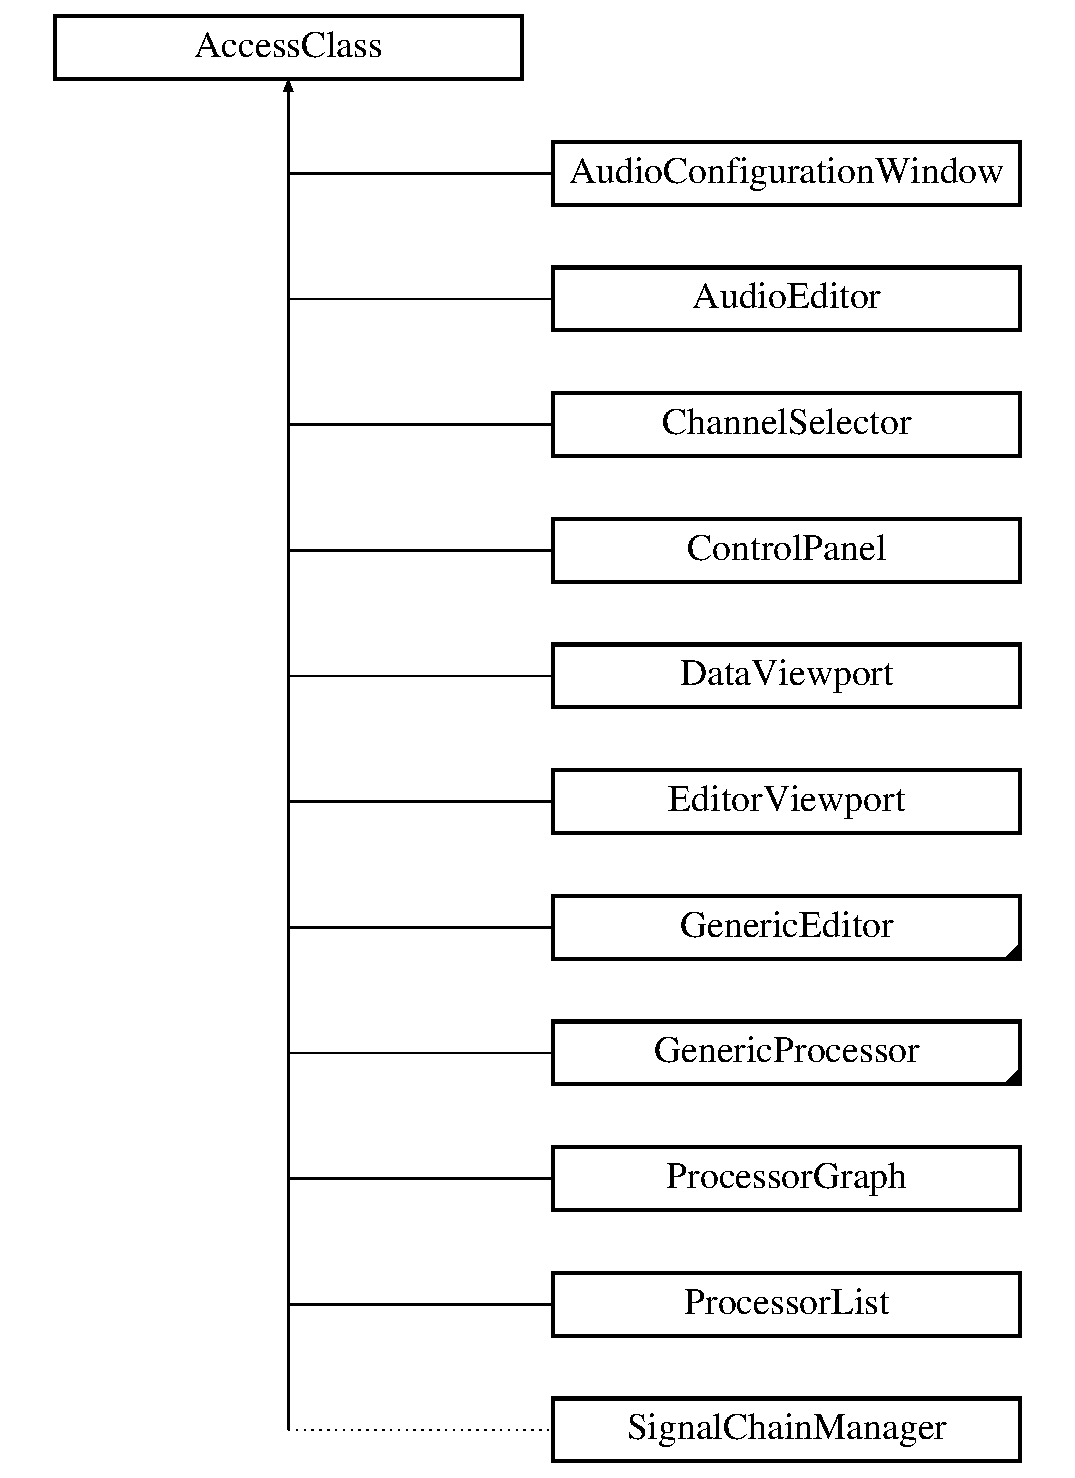
\includegraphics[height=12.000000cm]{classAccessClass}
\end{center}
\end{figure}
\subsection*{Public Member Functions}
\begin{DoxyCompactItemize}
\item 
\hypertarget{classAccessClass_ae6c601f53b3fd103bd7cd40f51c9c235}{void {\bfseries set\-U\-I\-Component} (\hyperlink{classUIComponent}{U\-I\-Component} $\ast$)}\label{classAccessClass_ae6c601f53b3fd103bd7cd40f51c9c235}

\item 
\hypertarget{classAccessClass_aa23dfab04264a78db261ccb8ac30f1ff}{virtual void {\bfseries update\-Child\-Components} ()}\label{classAccessClass_aa23dfab04264a78db261ccb8ac30f1ff}

\item 
\hypertarget{classAccessClass_a72bef8d5db8f8984f7b40f627a43998d}{\hyperlink{classEditorViewport}{Editor\-Viewport} $\ast$ {\bfseries get\-Editor\-Viewport} ()}\label{classAccessClass_a72bef8d5db8f8984f7b40f627a43998d}

\item 
\hypertarget{classAccessClass_a69500d6b6d466414e92eb9b31c8cb90d}{\hyperlink{classDataViewport}{Data\-Viewport} $\ast$ {\bfseries get\-Data\-Viewport} ()}\label{classAccessClass_a69500d6b6d466414e92eb9b31c8cb90d}

\item 
\hypertarget{classAccessClass_a18c4d1e45c74d6564d534bfe86bfc5da}{\hyperlink{classProcessorList}{Processor\-List} $\ast$ {\bfseries get\-Processor\-List} ()}\label{classAccessClass_a18c4d1e45c74d6564d534bfe86bfc5da}

\item 
\hypertarget{classAccessClass_abe0403e279f6047b2f307eaf9c913404}{\hyperlink{classProcessorGraph}{Processor\-Graph} $\ast$ {\bfseries get\-Processor\-Graph} ()}\label{classAccessClass_abe0403e279f6047b2f307eaf9c913404}

\item 
\hypertarget{classAccessClass_ae2559bca16f366b3b60bb64b062259cb}{\hyperlink{classControlPanel}{Control\-Panel} $\ast$ {\bfseries get\-Control\-Panel} ()}\label{classAccessClass_ae2559bca16f366b3b60bb64b062259cb}

\item 
\hypertarget{classAccessClass_abb4f62a65c45128a71eee802544fd3d1}{\hyperlink{classMessageCenter}{Message\-Center} $\ast$ {\bfseries get\-Message\-Center} ()}\label{classAccessClass_abb4f62a65c45128a71eee802544fd3d1}

\item 
\hypertarget{classAccessClass_a45bcba11a6ba8a754d76d6a3ee11fb26}{\hyperlink{classUIComponent}{U\-I\-Component} $\ast$ {\bfseries get\-U\-I\-Component} ()}\label{classAccessClass_a45bcba11a6ba8a754d76d6a3ee11fb26}

\item 
\hypertarget{classAccessClass_adca6f9ebbe535a03c024eb673a096972}{\hyperlink{classAudioComponent}{Audio\-Component} $\ast$ {\bfseries get\-Audio\-Component} ()}\label{classAccessClass_adca6f9ebbe535a03c024eb673a096972}

\end{DoxyCompactItemize}
\subsection*{Private Attributes}
\begin{DoxyCompactItemize}
\item 
\hypertarget{classAccessClass_a8d6f39cc955e6eb2f450bb377b7e23ca}{\hyperlink{classUIComponent}{U\-I\-Component} $\ast$ {\bfseries ui}}\label{classAccessClass_a8d6f39cc955e6eb2f450bb377b7e23ca}

\item 
\hypertarget{classAccessClass_a8732d9ac39d09ad512ad5d969a2f6388}{\hyperlink{classEditorViewport}{Editor\-Viewport} $\ast$ {\bfseries ev}}\label{classAccessClass_a8732d9ac39d09ad512ad5d969a2f6388}

\item 
\hypertarget{classAccessClass_a35894b8eb8810f3221c17f63f15c2406}{\hyperlink{classProcessorList}{Processor\-List} $\ast$ {\bfseries pl}}\label{classAccessClass_a35894b8eb8810f3221c17f63f15c2406}

\item 
\hypertarget{classAccessClass_ad518f5fc0a11e84473da5653505d8975}{\hyperlink{classDataViewport}{Data\-Viewport} $\ast$ {\bfseries dv}}\label{classAccessClass_ad518f5fc0a11e84473da5653505d8975}

\item 
\hypertarget{classAccessClass_a0f2a6b6031e117e17acf84f6816bfe3b}{\hyperlink{classProcessorGraph}{Processor\-Graph} $\ast$ {\bfseries pg}}\label{classAccessClass_a0f2a6b6031e117e17acf84f6816bfe3b}

\item 
\hypertarget{classAccessClass_a042707e5c002043506d4bf8744735077}{\hyperlink{classControlPanel}{Control\-Panel} $\ast$ {\bfseries cp}}\label{classAccessClass_a042707e5c002043506d4bf8744735077}

\item 
\hypertarget{classAccessClass_a948163dad2f276abb80524aab2b8d256}{\hyperlink{classMessageCenter}{Message\-Center} $\ast$ {\bfseries mc}}\label{classAccessClass_a948163dad2f276abb80524aab2b8d256}

\item 
\hypertarget{classAccessClass_aedc7ed8d7ef232bac40515fd87d5e7f5}{\hyperlink{classAudioComponent}{Audio\-Component} $\ast$ {\bfseries ac}}\label{classAccessClass_aedc7ed8d7ef232bac40515fd87d5e7f5}

\end{DoxyCompactItemize}


\subsection{Detailed Description}
Allows subclasses to access important pointers within the application.

\begin{DoxySeeAlso}{See also}
\hyperlink{classUIComponent}{U\-I\-Component} 
\end{DoxySeeAlso}


The documentation for this class was generated from the following file\-:\begin{DoxyCompactItemize}
\item 
Access\-Class.\-h\end{DoxyCompactItemize}

\hypertarget{classAudioComponent}{\section{Audio\-Component Class Reference}
\label{classAudioComponent}\index{Audio\-Component@{Audio\-Component}}
}


{\ttfamily \#include $<$Audio\-Component.\-h$>$}

\subsection*{Public Member Functions}
\begin{DoxyCompactItemize}
\item 
\hypertarget{classAudioComponent_a39ef696dde4891e20b17adb0c8057740}{void {\bfseries begin\-Callbacks} ()}\label{classAudioComponent_a39ef696dde4891e20b17adb0c8057740}

\item 
\hypertarget{classAudioComponent_a78e2a818d271fb26387d41875271e4ba}{void {\bfseries end\-Callbacks} ()}\label{classAudioComponent_a78e2a818d271fb26387d41875271e4ba}

\item 
\hypertarget{classAudioComponent_aaffe78d6dae978d9905cf2caf2f883b2}{void {\bfseries connect\-To\-Processor\-Graph} (Audio\-Processor\-Graph $\ast$processor\-Graph)}\label{classAudioComponent_aaffe78d6dae978d9905cf2caf2f883b2}

\item 
\hypertarget{classAudioComponent_a8570488c01bd73e836cfb1f153d7ec86}{void {\bfseries disconnect\-Processor\-Graph} ()}\label{classAudioComponent_a8570488c01bd73e836cfb1f153d7ec86}

\item 
\hypertarget{classAudioComponent_a5f6d992b7a5c267332416f8ee0b1aff0}{bool {\bfseries callbacks\-Are\-Active} ()}\label{classAudioComponent_a5f6d992b7a5c267332416f8ee0b1aff0}

\item 
\hypertarget{classAudioComponent_afa720e702e65def918da93505a4a9e7e}{void {\bfseries restart\-Device} ()}\label{classAudioComponent_afa720e702e65def918da93505a4a9e7e}

\item 
\hypertarget{classAudioComponent_ac85bf5472fbb1112b8429e26bcea6bc1}{void {\bfseries stop\-Device} ()}\label{classAudioComponent_ac85bf5472fbb1112b8429e26bcea6bc1}

\end{DoxyCompactItemize}
\subsection*{Public Attributes}
\begin{DoxyCompactItemize}
\item 
\hypertarget{classAudioComponent_a84f78369c478a8531a258ba8683033e1}{Audio\-Device\-Manager {\bfseries device\-Manager}}\label{classAudioComponent_a84f78369c478a8531a258ba8683033e1}

\end{DoxyCompactItemize}
\subsection*{Private Member Functions}
\begin{DoxyCompactItemize}
\item 
\hypertarget{classAudioComponent_a7a880353dbbe26c1e6ab830bea62d340}{{\bfseries J\-U\-C\-E\-\_\-\-D\-E\-C\-L\-A\-R\-E\-\_\-\-N\-O\-N\-\_\-\-C\-O\-P\-Y\-A\-B\-L\-E\-\_\-\-W\-I\-T\-H\-\_\-\-L\-E\-A\-K\-\_\-\-D\-E\-T\-E\-C\-T\-O\-R} (\hyperlink{classAudioComponent}{Audio\-Component})}\label{classAudioComponent_a7a880353dbbe26c1e6ab830bea62d340}

\end{DoxyCompactItemize}
\subsection*{Private Attributes}
\begin{DoxyCompactItemize}
\item 
\hypertarget{classAudioComponent_afc6f4562aa55d071a5f2a9607899ee91}{bool {\bfseries is\-Playing}}\label{classAudioComponent_afc6f4562aa55d071a5f2a9607899ee91}

\item 
\hypertarget{classAudioComponent_adebf82b36bfd76e3bfd9bbe3d40d4dad}{Audio\-Processor\-Player $\ast$ {\bfseries graph\-Player}}\label{classAudioComponent_adebf82b36bfd76e3bfd9bbe3d40d4dad}

\end{DoxyCompactItemize}


\subsection{Detailed Description}
Interfaces with system audio hardware.

Uses the audio card to generate the callbacks to run the \hyperlink{classProcessorGraph}{Processor\-Graph} during data acquisition.

Sends output to the audio card for audio monitoring.

Determines the initial size of the sample buffer (crucial for real-\/time feedback latency).

\begin{DoxySeeAlso}{See also}
\hyperlink{classMainWindow}{Main\-Window}, \hyperlink{classProcessorGraph}{Processor\-Graph} 
\end{DoxySeeAlso}


The documentation for this class was generated from the following file\-:\begin{DoxyCompactItemize}
\item 
Audio/Audio\-Component.\-h\end{DoxyCompactItemize}

\hypertarget{classAudioConfigurationWindow}{\section{Audio\-Configuration\-Window Class Reference}
\label{classAudioConfigurationWindow}\index{Audio\-Configuration\-Window@{Audio\-Configuration\-Window}}
}
Inheritance diagram for Audio\-Configuration\-Window\-:\begin{figure}[H]
\begin{center}
\leavevmode
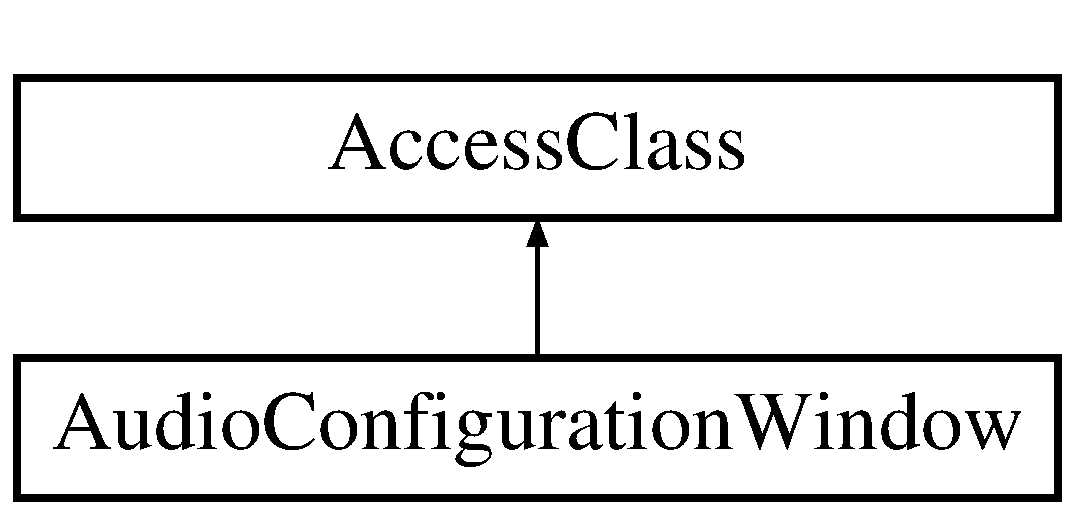
\includegraphics[height=2.000000cm]{classAudioConfigurationWindow}
\end{center}
\end{figure}
\subsection*{Public Member Functions}
\begin{DoxyCompactItemize}
\item 
\hypertarget{classAudioConfigurationWindow_af0cc726b42767b642bad85086cd29703}{{\bfseries Audio\-Configuration\-Window} (Audio\-Device\-Manager \&adm, Button $\ast$b)}\label{classAudioConfigurationWindow_af0cc726b42767b642bad85086cd29703}

\item 
\hypertarget{classAudioConfigurationWindow_a1e31b05a49ec2bbbcca7311dce8d0ad5}{void {\bfseries paint} (Graphics \&g)}\label{classAudioConfigurationWindow_a1e31b05a49ec2bbbcca7311dce8d0ad5}

\item 
\hypertarget{classAudioConfigurationWindow_a75dbdd5bc9773db08c692de134979641}{void {\bfseries resized} ()}\label{classAudioConfigurationWindow_a75dbdd5bc9773db08c692de134979641}

\end{DoxyCompactItemize}
\subsection*{Private Member Functions}
\begin{DoxyCompactItemize}
\item 
\hypertarget{classAudioConfigurationWindow_a6bb20e4ea9ead27b492609a1f3cbe313}{void {\bfseries close\-Button\-Pressed} ()}\label{classAudioConfigurationWindow_a6bb20e4ea9ead27b492609a1f3cbe313}

\end{DoxyCompactItemize}
\subsection*{Private Attributes}
\begin{DoxyCompactItemize}
\item 
\hypertarget{classAudioConfigurationWindow_a87e8cfa72ab2e33273d40971b98793dd}{Button $\ast$ {\bfseries control\-Button}}\label{classAudioConfigurationWindow_a87e8cfa72ab2e33273d40971b98793dd}

\end{DoxyCompactItemize}


The documentation for this class was generated from the following file\-:\begin{DoxyCompactItemize}
\item 
Processors/\-Editors/Audio\-Editor.\-h\end{DoxyCompactItemize}

\hypertarget{classAudioEditor}{\section{Audio\-Editor Class Reference}
\label{classAudioEditor}\index{Audio\-Editor@{Audio\-Editor}}
}
Inheritance diagram for Audio\-Editor\-:\begin{figure}[H]
\begin{center}
\leavevmode
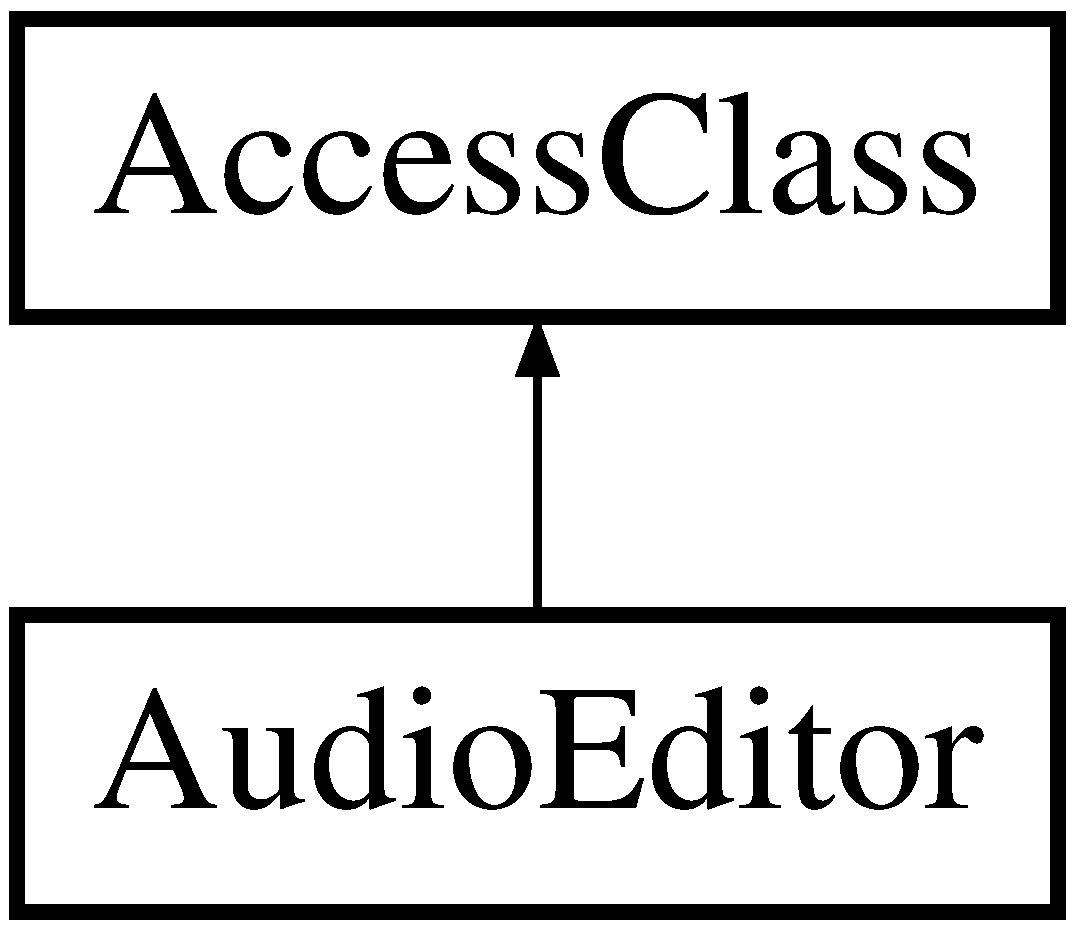
\includegraphics[height=2.000000cm]{classAudioEditor}
\end{center}
\end{figure}
\subsection*{Public Member Functions}
\begin{DoxyCompactItemize}
\item 
\hypertarget{classAudioEditor_a5be323528c200416d7f1e649a7f3bc30}{{\bfseries Audio\-Editor} (\hyperlink{classAudioNode}{Audio\-Node} $\ast$owner)}\label{classAudioEditor_a5be323528c200416d7f1e649a7f3bc30}

\item 
\hypertarget{classAudioEditor_af4aa4c78266e4a539c834a2e14154b90}{void {\bfseries paint} (Graphics \&g)}\label{classAudioEditor_af4aa4c78266e4a539c834a2e14154b90}

\item 
\hypertarget{classAudioEditor_a259636089a665bf4893e91735e524d4c}{bool {\bfseries key\-Pressed} (const Key\-Press \&key)}\label{classAudioEditor_a259636089a665bf4893e91735e524d4c}

\item 
\hypertarget{classAudioEditor_ada2c74ebc9cc51859e04cdc6898acc67}{void {\bfseries resized} ()}\label{classAudioEditor_ada2c74ebc9cc51859e04cdc6898acc67}

\end{DoxyCompactItemize}
\subsection*{Private Member Functions}
\begin{DoxyCompactItemize}
\item 
\hypertarget{classAudioEditor_a5449ebec2dabddad876dbbbd7f8fa424}{void {\bfseries button\-Clicked} (Button $\ast$button)}\label{classAudioEditor_a5449ebec2dabddad876dbbbd7f8fa424}

\item 
\hypertarget{classAudioEditor_af226bb0a6c971cd3454d75fa9aba29ca}{void {\bfseries slider\-Value\-Changed} (Slider $\ast$slider)}\label{classAudioEditor_af226bb0a6c971cd3454d75fa9aba29ca}

\item 
\hypertarget{classAudioEditor_a2fae9b7f8defa2e2f5d0f54c5505295f}{{\bfseries J\-U\-C\-E\-\_\-\-D\-E\-C\-L\-A\-R\-E\-\_\-\-N\-O\-N\-\_\-\-C\-O\-P\-Y\-A\-B\-L\-E\-\_\-\-W\-I\-T\-H\-\_\-\-L\-E\-A\-K\-\_\-\-D\-E\-T\-E\-C\-T\-O\-R} (\hyperlink{classAudioEditor}{Audio\-Editor})}\label{classAudioEditor_a2fae9b7f8defa2e2f5d0f54c5505295f}

\end{DoxyCompactItemize}
\subsection*{Private Attributes}
\begin{DoxyCompactItemize}
\item 
\hypertarget{classAudioEditor_abf448cf9e86bb877cae8fc45341e9b34}{float {\bfseries last\-Value}}\label{classAudioEditor_abf448cf9e86bb877cae8fc45341e9b34}

\item 
\hypertarget{classAudioEditor_a61fba4d0fe0c10fb251a895e0bd7416c}{\hyperlink{classMuteButton}{Mute\-Button} $\ast$ {\bfseries mute\-Button}}\label{classAudioEditor_a61fba4d0fe0c10fb251a895e0bd7416c}

\item 
\hypertarget{classAudioEditor_aa49403b405b8eaa56118f4464a9a18cb}{\hyperlink{classAudioWindowButton}{Audio\-Window\-Button} $\ast$ {\bfseries audio\-Window\-Button}}\label{classAudioEditor_aa49403b405b8eaa56118f4464a9a18cb}

\item 
\hypertarget{classAudioEditor_a54bb47012b71f96a69d5acbe91e992cd}{\hyperlink{classAudioConfigurationWindow}{Audio\-Configuration\-Window} $\ast$ {\bfseries acw}}\label{classAudioEditor_a54bb47012b71f96a69d5acbe91e992cd}

\item 
\hypertarget{classAudioEditor_a19b1e6de95cdd4da935ab9e5cfcce006}{Slider $\ast$ {\bfseries volume\-Slider}}\label{classAudioEditor_a19b1e6de95cdd4da935ab9e5cfcce006}

\end{DoxyCompactItemize}


The documentation for this class was generated from the following file\-:\begin{DoxyCompactItemize}
\item 
Processors/\-Editors/Audio\-Editor.\-h\end{DoxyCompactItemize}

\hypertarget{classAudioNode}{\section{Audio\-Node Class Reference}
\label{classAudioNode}\index{Audio\-Node@{Audio\-Node}}
}
Inheritance diagram for Audio\-Node\-:\begin{figure}[H]
\begin{center}
\leavevmode
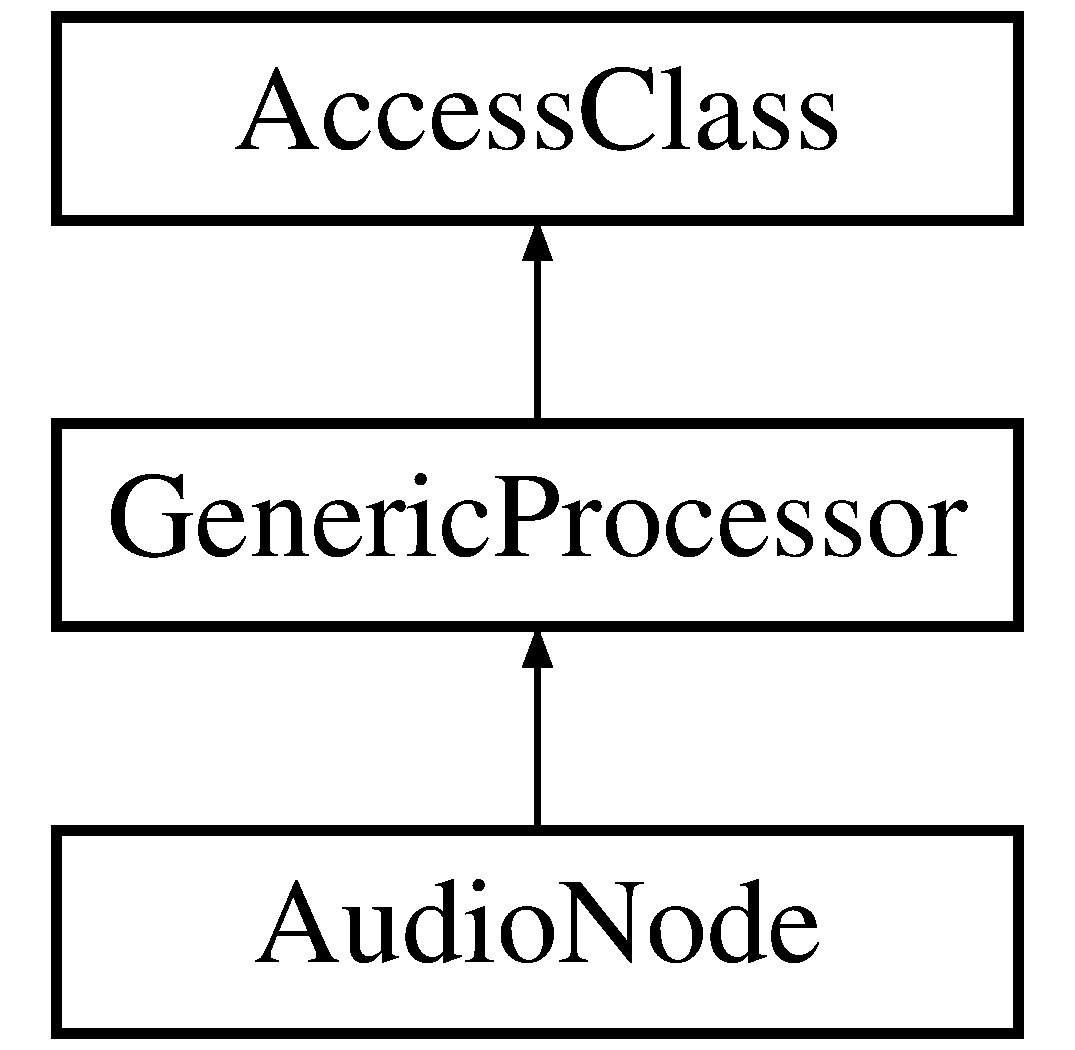
\includegraphics[height=3.000000cm]{classAudioNode}
\end{center}
\end{figure}
\subsection*{Public Member Functions}
\begin{DoxyCompactItemize}
\item 
\hypertarget{classAudioNode_a90d23dc83c27a5ff3a8e5029a5498b35}{void {\bfseries process} (Audio\-Sample\-Buffer \&buffer, Midi\-Buffer \&midi\-Messages, int \&n\-Samples)}\label{classAudioNode_a90d23dc83c27a5ff3a8e5029a5498b35}

\item 
\hypertarget{classAudioNode_a61ca4c81f908093001fd7805951274a2}{void {\bfseries set\-Parameter} (int parameter\-Index, float new\-Value)}\label{classAudioNode_a61ca4c81f908093001fd7805951274a2}

\item 
\hypertarget{classAudioNode_a46c720536cf4b8502d841a65f9dccd1d}{Audio\-Processor\-Editor $\ast$ {\bfseries create\-Editor} ()}\label{classAudioNode_a46c720536cf4b8502d841a65f9dccd1d}

\item 
\hypertarget{classAudioNode_a66b3cdf827054c9fdcdc667918a1f159}{void {\bfseries set\-Channel\-Status} (int, bool)}\label{classAudioNode_a66b3cdf827054c9fdcdc667918a1f159}

\item 
\hypertarget{classAudioNode_ae3ac34b77bc9663868c5739cb891d1a8}{bool {\bfseries is\-Audio\-Or\-Record\-Node} ()}\label{classAudioNode_ae3ac34b77bc9663868c5739cb891d1a8}

\item 
\hypertarget{classAudioNode_a94937d356ee86b72eed82fad0337f9e7}{void {\bfseries enable\-Current\-Channel} (bool)}\label{classAudioNode_a94937d356ee86b72eed82fad0337f9e7}

\end{DoxyCompactItemize}
\subsection*{Public Attributes}
\begin{DoxyCompactItemize}
\item 
\hypertarget{classAudioNode_a23fc8aba3a18b99825bed4836eb6f647}{Scoped\-Pointer$<$ \hyperlink{classAudioEditor}{Audio\-Editor} $>$ {\bfseries audio\-Editor}}\label{classAudioNode_a23fc8aba3a18b99825bed4836eb6f647}

\end{DoxyCompactItemize}
\subsection*{Private Member Functions}
\begin{DoxyCompactItemize}
\item 
\hypertarget{classAudioNode_af61664bac9bbf287c15f909b70fadc5e}{{\bfseries J\-U\-C\-E\-\_\-\-D\-E\-C\-L\-A\-R\-E\-\_\-\-N\-O\-N\-\_\-\-C\-O\-P\-Y\-A\-B\-L\-E\-\_\-\-W\-I\-T\-H\-\_\-\-L\-E\-A\-K\-\_\-\-D\-E\-T\-E\-C\-T\-O\-R} (\hyperlink{classAudioNode}{Audio\-Node})}\label{classAudioNode_af61664bac9bbf287c15f909b70fadc5e}

\end{DoxyCompactItemize}
\subsection*{Private Attributes}
\begin{DoxyCompactItemize}
\item 
\hypertarget{classAudioNode_a751bace950ee0682227d0b488e8fd71b}{Array$<$ int $>$ {\bfseries left\-Chan}}\label{classAudioNode_a751bace950ee0682227d0b488e8fd71b}

\item 
\hypertarget{classAudioNode_a8e0286ba3263d2a4ad84c8c51cab98f6}{Array$<$ int $>$ {\bfseries right\-Chan}}\label{classAudioNode_a8e0286ba3263d2a4ad84c8c51cab98f6}

\item 
\hypertarget{classAudioNode_ab269ffd3dc0f501984db1be343f9f70d}{float {\bfseries volume}}\label{classAudioNode_ab269ffd3dc0f501984db1be343f9f70d}

\end{DoxyCompactItemize}
\subsection*{Additional Inherited Members}


The documentation for this class was generated from the following file\-:\begin{DoxyCompactItemize}
\item 
Processors/Audio\-Node.\-h\end{DoxyCompactItemize}

\hypertarget{classAudioWindowButton}{\section{Audio\-Window\-Button Class Reference}
\label{classAudioWindowButton}\index{Audio\-Window\-Button@{Audio\-Window\-Button}}
}
\subsection*{Public Member Functions}
\begin{DoxyCompactItemize}
\item 
\hypertarget{classAudioWindowButton_a9970fe887c1f35f09d98c43b98ca2754}{void {\bfseries paint\-Button} (Graphics \&g, bool is\-Mouse\-Over, bool is\-Button\-Down)}\label{classAudioWindowButton_a9970fe887c1f35f09d98c43b98ca2754}

\end{DoxyCompactItemize}
\subsection*{Private Attributes}
\begin{DoxyCompactItemize}
\item 
\hypertarget{classAudioWindowButton_adf671a87ab6c84be204d66c36f77d7f9}{Font {\bfseries font}}\label{classAudioWindowButton_adf671a87ab6c84be204d66c36f77d7f9}

\end{DoxyCompactItemize}


The documentation for this class was generated from the following file\-:\begin{DoxyCompactItemize}
\item 
Processors/\-Editors/Audio\-Editor.\-h\end{DoxyCompactItemize}

\hypertarget{classBaseUIElement}{\section{Base\-U\-I\-Element Class Reference}
\label{classBaseUIElement}\index{Base\-U\-I\-Element@{Base\-U\-I\-Element}}
}
Inheritance diagram for Base\-U\-I\-Element\-:\begin{figure}[H]
\begin{center}
\leavevmode
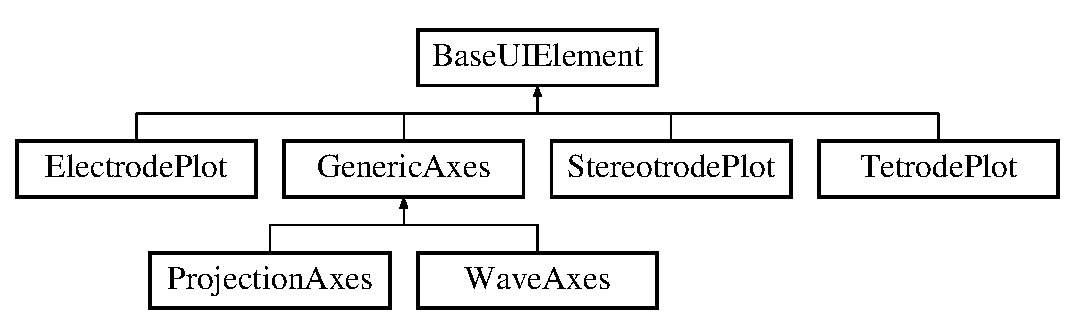
\includegraphics[height=3.000000cm]{classBaseUIElement}
\end{center}
\end{figure}
\subsection*{Public Member Functions}
\begin{DoxyCompactItemize}
\item 
\hypertarget{classBaseUIElement_a504a9fc6aa113993c16e24d2a128b383}{{\bfseries Base\-U\-I\-Element} (int x, int y, double w, double h)}\label{classBaseUIElement_a504a9fc6aa113993c16e24d2a128b383}

\item 
\hypertarget{classBaseUIElement_a788f73bf664936f6140525e7870927b7}{{\bfseries Base\-U\-I\-Element} (int x, int y, double w, double h, int p)}\label{classBaseUIElement_a788f73bf664936f6140525e7870927b7}

\item 
\hypertarget{classBaseUIElement_a8e39a18f63d75f2c790b57e1639c984b}{virtual void {\bfseries redraw} ()}\label{classBaseUIElement_a8e39a18f63d75f2c790b57e1639c984b}

\item 
\hypertarget{classBaseUIElement_acb89742a813bbb3c564bdeeca82f5ec1}{void {\bfseries draw\-Element\-Edges} ()}\label{classBaseUIElement_acb89742a813bbb3c564bdeeca82f5ec1}

\item 
\hypertarget{classBaseUIElement_a474f083d9b09d0aa0ad81a861c440179}{virtual void {\bfseries set\-Enabled} (bool e)}\label{classBaseUIElement_a474f083d9b09d0aa0ad81a861c440179}

\item 
\hypertarget{classBaseUIElement_a560672179cd7a782c76f520e9b7ecc29}{virtual bool {\bfseries get\-Enabled} ()}\label{classBaseUIElement_a560672179cd7a782c76f520e9b7ecc29}

\item 
\hypertarget{classBaseUIElement_a6387aa84bf1c2893f850041684c34640}{virtual void {\bfseries set\-Position} (int x, int y, double w, double h)}\label{classBaseUIElement_a6387aa84bf1c2893f850041684c34640}

\item 
\hypertarget{classBaseUIElement_a83102b6dd32ab18487d0c222e4c49b37}{virtual void {\bfseries set\-Position} (int, int)}\label{classBaseUIElement_a83102b6dd32ab18487d0c222e4c49b37}

\item 
\hypertarget{classBaseUIElement_ac26f4c69ee4d1a2b1a822efd5a10ee93}{virtual void {\bfseries get\-Position} (int $\ast$, int $\ast$, double $\ast$, double $\ast$)}\label{classBaseUIElement_ac26f4c69ee4d1a2b1a822efd5a10ee93}

\item 
\hypertarget{classBaseUIElement_a8f8022d087c697c5a04c10417ea1ca20}{double {\bfseries get\-Height} ()}\label{classBaseUIElement_a8f8022d087c697c5a04c10417ea1ca20}

\item 
\hypertarget{classBaseUIElement_ae32de848136eca61c71830aa8b48ed95}{double {\bfseries get\-Width} ()}\label{classBaseUIElement_ae32de848136eca61c71830aa8b48ed95}

\item 
\hypertarget{classBaseUIElement_a74aa4569d1c6e3edbad13b7f29de8d56}{int {\bfseries get\-X} ()}\label{classBaseUIElement_a74aa4569d1c6e3edbad13b7f29de8d56}

\item 
\hypertarget{classBaseUIElement_a6e512068c7a0b1c0aa6b1e04bd72d5a7}{int {\bfseries get\-Y} ()}\label{classBaseUIElement_a6e512068c7a0b1c0aa6b1e04bd72d5a7}

\item 
\hypertarget{classBaseUIElement_a20e0a11922c3290dc85e64e13fa86b65}{virtual void {\bfseries process\-Spike\-Object} (\hyperlink{structSpikeObject}{Spike\-Object} s)}\label{classBaseUIElement_a20e0a11922c3290dc85e64e13fa86b65}

\item 
\hypertarget{classBaseUIElement_a80bf90bc03c8c39f71b523f7f5735ab0}{virtual void {\bfseries pan} (int, bool)}\label{classBaseUIElement_a80bf90bc03c8c39f71b523f7f5735ab0}

\item 
\hypertarget{classBaseUIElement_ab3777efcbb469ba0050f1cdd9fcfc1f1}{virtual void {\bfseries zoom} (int, bool)}\label{classBaseUIElement_ab3777efcbb469ba0050f1cdd9fcfc1f1}

\item 
\hypertarget{classBaseUIElement_a5c498c11811c0ef30e7dce0cf71dd386}{virtual void {\bfseries clear} ()}\label{classBaseUIElement_a5c498c11811c0ef30e7dce0cf71dd386}

\item 
\hypertarget{classBaseUIElement_aa064979e30e4573dd5d477e2dda0cbd7}{bool {\bfseries hit\-Test} (int x, int y)}\label{classBaseUIElement_aa064979e30e4573dd5d477e2dda0cbd7}

\end{DoxyCompactItemize}
\subsection*{Protected Member Functions}
\begin{DoxyCompactItemize}
\item 
\hypertarget{classBaseUIElement_a01f712833dbbdfc29fc8614eb34e79e5}{void {\bfseries set\-Gl\-Viewport} ()}\label{classBaseUIElement_a01f712833dbbdfc29fc8614eb34e79e5}

\end{DoxyCompactItemize}
\subsection*{Protected Attributes}
\begin{DoxyCompactItemize}
\item 
\hypertarget{classBaseUIElement_ad65449ac10a833a2ecf48315b17bfbba}{int {\bfseries xpos}}\label{classBaseUIElement_ad65449ac10a833a2ecf48315b17bfbba}

\item 
\hypertarget{classBaseUIElement_a730d67d2f53f256ffcd2caf2db166f59}{int {\bfseries ypos}}\label{classBaseUIElement_a730d67d2f53f256ffcd2caf2db166f59}

\item 
\hypertarget{classBaseUIElement_a23a5dcf0e8fe642f779b0fe73f02584f}{int {\bfseries y\-Offset}}\label{classBaseUIElement_a23a5dcf0e8fe642f779b0fe73f02584f}

\item 
\hypertarget{classBaseUIElement_a4fc207e53cafb2e7a072ba1ea931eff3}{double {\bfseries height}}\label{classBaseUIElement_a4fc207e53cafb2e7a072ba1ea931eff3}

\item 
\hypertarget{classBaseUIElement_a913b0634330b02a5aa2d0dad22982cc4}{double {\bfseries width}}\label{classBaseUIElement_a913b0634330b02a5aa2d0dad22982cc4}

\item 
\hypertarget{classBaseUIElement_acb44180764682ab3f5690373549e4cae}{bool {\bfseries enabled}}\label{classBaseUIElement_acb44180764682ab3f5690373549e4cae}

\item 
\hypertarget{classBaseUIElement_a4dca2aac9fd607791c7702d8fedb4bb2}{double {\bfseries padding}}\label{classBaseUIElement_a4dca2aac9fd607791c7702d8fedb4bb2}

\end{DoxyCompactItemize}


The documentation for this class was generated from the following file\-:\begin{DoxyCompactItemize}
\item 
Processors/\-Visualization/\-Spike\-Plotting/Base\-U\-I\-Element.\-h\end{DoxyCompactItemize}

\hypertarget{structRecordNode_1_1Channel}{\section{Record\-Node\-:\-:Channel Struct Reference}
\label{structRecordNode_1_1Channel}\index{Record\-Node\-::\-Channel@{Record\-Node\-::\-Channel}}
}
\subsection*{Public Attributes}
\begin{DoxyCompactItemize}
\item 
\hypertarget{structRecordNode_1_1Channel_ac8a38f96771e58f1710969ee1c4e81bc}{int {\bfseries node\-Id}}\label{structRecordNode_1_1Channel_ac8a38f96771e58f1710969ee1c4e81bc}

\item 
\hypertarget{structRecordNode_1_1Channel_af29847633746e201d14acdd316531c24}{int {\bfseries chan}}\label{structRecordNode_1_1Channel_af29847633746e201d14acdd316531c24}

\item 
\hypertarget{structRecordNode_1_1Channel_a7cde8d8153a509a2d1a33c35e2038452}{String {\bfseries name}}\label{structRecordNode_1_1Channel_a7cde8d8153a509a2d1a33c35e2038452}

\item 
\hypertarget{structRecordNode_1_1Channel_a729b53960f427ee5b8fa553af24d89f2}{bool {\bfseries is\-Recording}}\label{structRecordNode_1_1Channel_a729b53960f427ee5b8fa553af24d89f2}

\item 
\hypertarget{structRecordNode_1_1Channel_a17ee4d040024a5fb777479ca3c89cdc7}{String {\bfseries filename}}\label{structRecordNode_1_1Channel_a17ee4d040024a5fb777479ca3c89cdc7}

\item 
\hypertarget{structRecordNode_1_1Channel_ae9bc431717c4a8d8ae2b498c210791f0}{F\-I\-L\-E $\ast$ {\bfseries file}}\label{structRecordNode_1_1Channel_ae9bc431717c4a8d8ae2b498c210791f0}

\end{DoxyCompactItemize}


\subsection{Detailed Description}
Holds information for a given channel to be recorded to its own file. 

The documentation for this struct was generated from the following file\-:\begin{DoxyCompactItemize}
\item 
Processors/Record\-Node.\-h\end{DoxyCompactItemize}

\hypertarget{classChannelSelector}{\section{Channel\-Selector Class Reference}
\label{classChannelSelector}\index{Channel\-Selector@{Channel\-Selector}}
}
Inheritance diagram for Channel\-Selector\-:\begin{figure}[H]
\begin{center}
\leavevmode
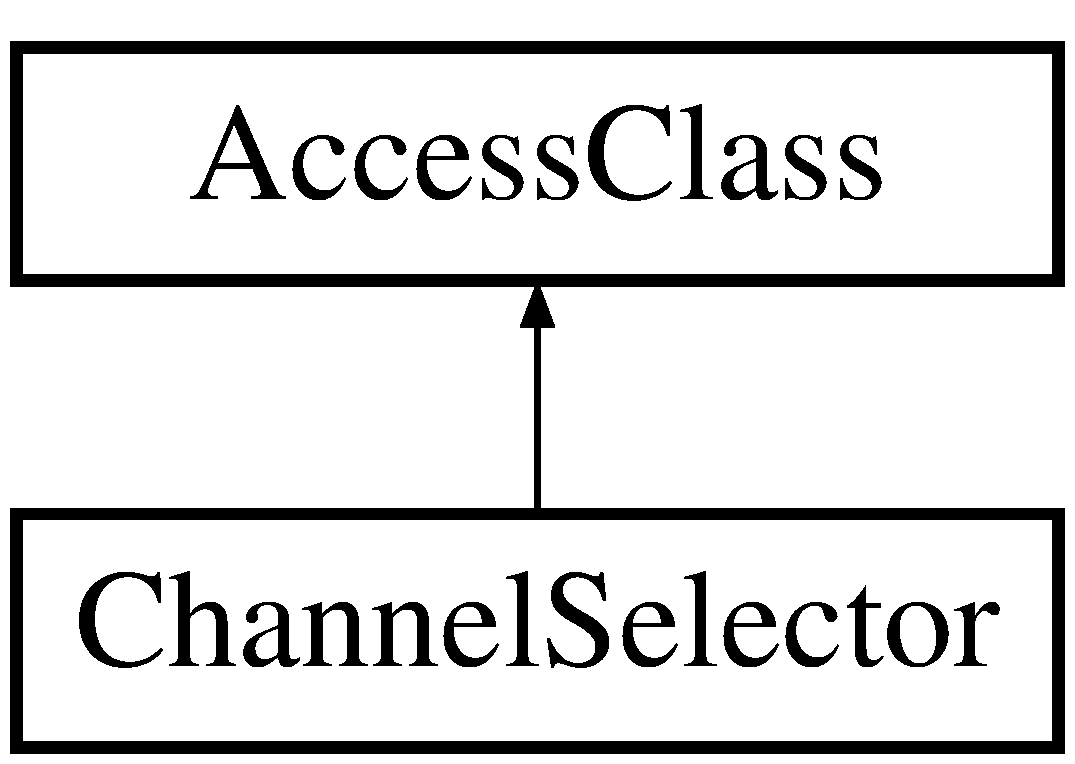
\includegraphics[height=2.000000cm]{classChannelSelector}
\end{center}
\end{figure}
\subsection*{Public Member Functions}
\begin{DoxyCompactItemize}
\item 
\hyperlink{classChannelSelector_a593fc6e836661a86e0ca788bffdb4d24}{Channel\-Selector} (bool create\-Buttons, Font \&title\-Font)
\item 
\hyperlink{classChannelSelector_a918cd253d71e3a26e6b6bb8b1be52eed}{$\sim$\-Channel\-Selector} ()
\item 
void \hyperlink{classChannelSelector_afe0c3299f08f26d6872a7bfe6b20069e}{button\-Clicked} (Button $\ast$button)
\item 
Array$<$ int $>$ \hyperlink{classChannelSelector_ad2397a6d709a0ef783527e4c5f2fbf9f}{get\-Active\-Channels} ()
\item 
void \hyperlink{classChannelSelector_a30faca8ee72022f68e2ea776453f801a}{set\-Active\-Channels} (Array$<$ int $>$)
\item 
void \hyperlink{classChannelSelector_a717956a6b754e1aa157371851c396c79}{set\-Num\-Channels} (int)
\item 
bool \hyperlink{classChannelSelector_a1de299562edcbc0d4249a7fc5d22917f}{get\-Record\-Status} (int chan)
\item 
bool \hyperlink{classChannelSelector_a846b95d112e09cec70d426a80731eda5}{get\-Audio\-Status} (int chan)
\item 
int \hyperlink{classChannelSelector_a7865695da614c8ee1e3106c545dd12f4}{get\-Desired\-Width} ()
\item 
\hypertarget{classChannelSelector_a53d43af4d197bd3def9c96b0c98811e2}{void {\bfseries inactivate\-Buttons} ()}\label{classChannelSelector_a53d43af4d197bd3def9c96b0c98811e2}

\item 
\hypertarget{classChannelSelector_adcc831c5ba479d04df8ee711f169311d}{void {\bfseries activate\-Buttons} ()}\label{classChannelSelector_adcc831c5ba479d04df8ee711f169311d}

\item 
\hypertarget{classChannelSelector_ae4fc9b23915004fb4f1ade854e7dddb4}{void {\bfseries set\-Radio\-Status} (bool)}\label{classChannelSelector_ae4fc9b23915004fb4f1ade854e7dddb4}

\item 
\hypertarget{classChannelSelector_a10b3542c4c5f2815b663692649b69eea}{void {\bfseries param\-Buttons\-Toggled\-By\-Default} (bool t)}\label{classChannelSelector_a10b3542c4c5f2815b663692649b69eea}

\end{DoxyCompactItemize}
\subsection*{Public Attributes}
\begin{DoxyCompactItemize}
\item 
\hypertarget{classChannelSelector_aa3a3c5a34e0c20248c1283acc0e91e3d}{bool {\bfseries events\-Only}}\label{classChannelSelector_aa3a3c5a34e0c20248c1283acc0e91e3d}

\end{DoxyCompactItemize}
\subsection*{Private Types}
\begin{DoxyCompactItemize}
\item 
enum \{ {\bfseries A\-U\-D\-I\-O}, 
{\bfseries R\-E\-C\-O\-R\-D}, 
{\bfseries P\-A\-R\-A\-M\-E\-T\-E\-R}
 \}
\end{DoxyCompactItemize}
\subsection*{Private Member Functions}
\begin{DoxyCompactItemize}
\item 
\hypertarget{classChannelSelector_acdc19312c258596a5786983526f8d5da}{void {\bfseries resized} ()}\label{classChannelSelector_acdc19312c258596a5786983526f8d5da}

\item 
\hypertarget{classChannelSelector_a05c5201380ab52ab9b310fcbb4ed11df}{void {\bfseries add\-Button} ()}\label{classChannelSelector_a05c5201380ab52ab9b310fcbb4ed11df}

\item 
\hypertarget{classChannelSelector_a999257dab86b930e09e64227e65b1c6a}{void {\bfseries remove\-Button} ()}\label{classChannelSelector_a999257dab86b930e09e64227e65b1c6a}

\item 
\hypertarget{classChannelSelector_a0b1994f1bc6978c452be67441f988144}{void {\bfseries refresh\-Button\-Boundaries} ()}\label{classChannelSelector_a0b1994f1bc6978c452be67441f988144}

\item 
\hypertarget{classChannelSelector_a0d7c58692724a9a47afbd2eea26f6453}{void {\bfseries timer\-Callback} ()}\label{classChannelSelector_a0d7c58692724a9a47afbd2eea26f6453}

\item 
\hypertarget{classChannelSelector_aa9a1eb97aa4f3760fb3777b50f7aac83}{void {\bfseries paint} (Graphics \&g)}\label{classChannelSelector_aa9a1eb97aa4f3760fb3777b50f7aac83}

\end{DoxyCompactItemize}
\subsection*{Private Attributes}
\begin{DoxyCompactItemize}
\item 
\hypertarget{classChannelSelector_a125d243727b3c6eb3a3e805d393ff655}{\hyperlink{classEditorButton}{Editor\-Button} $\ast$ {\bfseries audio\-Button}}\label{classChannelSelector_a125d243727b3c6eb3a3e805d393ff655}

\item 
\hypertarget{classChannelSelector_ad5613602460b2a19bd0c6e720488c406}{\hyperlink{classEditorButton}{Editor\-Button} $\ast$ {\bfseries record\-Button}}\label{classChannelSelector_ad5613602460b2a19bd0c6e720488c406}

\item 
\hypertarget{classChannelSelector_a1d83f4095fbeec31e17cd8ad9211c2d4}{\hyperlink{classEditorButton}{Editor\-Button} $\ast$ {\bfseries params\-Button}}\label{classChannelSelector_a1d83f4095fbeec31e17cd8ad9211c2d4}

\item 
\hypertarget{classChannelSelector_a0d3097d2e792c9b61a1977d49c43e9a9}{\hyperlink{classEditorButton}{Editor\-Button} $\ast$ {\bfseries all\-Button}}\label{classChannelSelector_a0d3097d2e792c9b61a1977d49c43e9a9}

\item 
\hypertarget{classChannelSelector_a4bad9aed3443274ab65b227f48e1d2a3}{\hyperlink{classEditorButton}{Editor\-Button} $\ast$ {\bfseries none\-Button}}\label{classChannelSelector_a4bad9aed3443274ab65b227f48e1d2a3}

\item 
\hypertarget{classChannelSelector_a90f23d0226bfeb29ea5d261bb602be9b}{Array$<$ \hyperlink{classChannelSelectorButton}{Channel\-Selector\-Button} $\ast$ $>$ {\bfseries parameter\-Buttons}}\label{classChannelSelector_a90f23d0226bfeb29ea5d261bb602be9b}

\item 
\hypertarget{classChannelSelector_ac50e843be255ca04b83a4d28907511a1}{Array$<$ \hyperlink{classChannelSelectorButton}{Channel\-Selector\-Button} $\ast$ $>$ {\bfseries audio\-Buttons}}\label{classChannelSelector_ac50e843be255ca04b83a4d28907511a1}

\item 
\hypertarget{classChannelSelector_ae7cbcfb0a437434a59077847cbf48360}{Array$<$ \hyperlink{classChannelSelectorButton}{Channel\-Selector\-Button} $\ast$ $>$ {\bfseries record\-Buttons}}\label{classChannelSelector_ae7cbcfb0a437434a59077847cbf48360}

\item 
\hypertarget{classChannelSelector_ab71b9a6f51948339fa8cc02622bd4bac}{bool {\bfseries params\-Toggled}}\label{classChannelSelector_ab71b9a6f51948339fa8cc02622bd4bac}

\item 
\hypertarget{classChannelSelector_a7548f321c4c91a64fea36d62854d5459}{bool {\bfseries params\-Active}}\label{classChannelSelector_a7548f321c4c91a64fea36d62854d5459}

\item 
\hypertarget{classChannelSelector_adaed7f23325155b9c11138dd2bbcaad0}{bool {\bfseries radio\-Status}}\label{classChannelSelector_adaed7f23325155b9c11138dd2bbcaad0}

\item 
\hypertarget{classChannelSelector_abfc6c6199895c7303606af884fa65b3f}{bool {\bfseries is\-Not\-Sink}}\label{classChannelSelector_abfc6c6199895c7303606af884fa65b3f}

\item 
\hypertarget{classChannelSelector_a780d94efaf61716df4b3a4b6d9e98376}{bool {\bfseries move\-Right}}\label{classChannelSelector_a780d94efaf61716df4b3a4b6d9e98376}

\item 
\hypertarget{classChannelSelector_ab6442cee85bfbab885bec0e1c91d85de}{bool {\bfseries move\-Left}}\label{classChannelSelector_ab6442cee85bfbab885bec0e1c91d85de}

\item 
\hypertarget{classChannelSelector_acdfddce909bd2d5ea67437d7b21782d7}{int {\bfseries offset\-L\-R}}\label{classChannelSelector_acdfddce909bd2d5ea67437d7b21782d7}

\item 
\hypertarget{classChannelSelector_ae81b21b00c4e19045b4becb7a856aec9}{int {\bfseries offset\-U\-D}}\label{classChannelSelector_ae81b21b00c4e19045b4becb7a856aec9}

\item 
\hypertarget{classChannelSelector_a83a2b3f79caa247f61e29b5f67ef3582}{int {\bfseries parameter\-Offset}}\label{classChannelSelector_a83a2b3f79caa247f61e29b5f67ef3582}

\item 
\hypertarget{classChannelSelector_a42a3b8d0333e186f44cfc09deb4771cf}{int {\bfseries audio\-Offset}}\label{classChannelSelector_a42a3b8d0333e186f44cfc09deb4771cf}

\item 
\hypertarget{classChannelSelector_a324c95cbb8a3bcaa6304f533dce9040c}{int {\bfseries record\-Offset}}\label{classChannelSelector_a324c95cbb8a3bcaa6304f533dce9040c}

\item 
\hypertarget{classChannelSelector_a60c31518c310f5ec8fb1aa5f6af0110b}{int {\bfseries desired\-Offset}}\label{classChannelSelector_a60c31518c310f5ec8fb1aa5f6af0110b}

\item 
\hypertarget{classChannelSelector_aaa491ce371b18cdc6974d377ed8c06ad}{Font \& {\bfseries title\-Font}}\label{classChannelSelector_aaa491ce371b18cdc6974d377ed8c06ad}

\end{DoxyCompactItemize}


\subsection{Constructor \& Destructor Documentation}
\hypertarget{classChannelSelector_a593fc6e836661a86e0ca788bffdb4d24}{\index{Channel\-Selector@{Channel\-Selector}!Channel\-Selector@{Channel\-Selector}}
\index{Channel\-Selector@{Channel\-Selector}!ChannelSelector@{Channel\-Selector}}
\subsubsection[{Channel\-Selector}]{\setlength{\rightskip}{0pt plus 5cm}Channel\-Selector\-::\-Channel\-Selector (
\begin{DoxyParamCaption}
\item[{bool}]{create\-Buttons, }
\item[{Font \&}]{title\-Font}
\end{DoxyParamCaption}
)}}\label{classChannelSelector_a593fc6e836661a86e0ca788bffdb4d24}
constructor \hypertarget{classChannelSelector_a918cd253d71e3a26e6b6bb8b1be52eed}{\index{Channel\-Selector@{Channel\-Selector}!$\sim$\-Channel\-Selector@{$\sim$\-Channel\-Selector}}
\index{$\sim$\-Channel\-Selector@{$\sim$\-Channel\-Selector}!ChannelSelector@{Channel\-Selector}}
\subsubsection[{$\sim$\-Channel\-Selector}]{\setlength{\rightskip}{0pt plus 5cm}Channel\-Selector\-::$\sim$\-Channel\-Selector (
\begin{DoxyParamCaption}
{}
\end{DoxyParamCaption}
)}}\label{classChannelSelector_a918cd253d71e3a26e6b6bb8b1be52eed}
destructor 

\subsection{Member Function Documentation}
\hypertarget{classChannelSelector_afe0c3299f08f26d6872a7bfe6b20069e}{\index{Channel\-Selector@{Channel\-Selector}!button\-Clicked@{button\-Clicked}}
\index{button\-Clicked@{button\-Clicked}!ChannelSelector@{Channel\-Selector}}
\subsubsection[{button\-Clicked}]{\setlength{\rightskip}{0pt plus 5cm}void Channel\-Selector\-::button\-Clicked (
\begin{DoxyParamCaption}
\item[{Button $\ast$}]{button}
\end{DoxyParamCaption}
)}}\label{classChannelSelector_afe0c3299f08f26d6872a7bfe6b20069e}
button callback \hypertarget{classChannelSelector_ad2397a6d709a0ef783527e4c5f2fbf9f}{\index{Channel\-Selector@{Channel\-Selector}!get\-Active\-Channels@{get\-Active\-Channels}}
\index{get\-Active\-Channels@{get\-Active\-Channels}!ChannelSelector@{Channel\-Selector}}
\subsubsection[{get\-Active\-Channels}]{\setlength{\rightskip}{0pt plus 5cm}Array$<$int$>$ Channel\-Selector\-::get\-Active\-Channels (
\begin{DoxyParamCaption}
{}
\end{DoxyParamCaption}
)}}\label{classChannelSelector_ad2397a6d709a0ef783527e4c5f2fbf9f}
Return an array of selected channels. \hypertarget{classChannelSelector_a846b95d112e09cec70d426a80731eda5}{\index{Channel\-Selector@{Channel\-Selector}!get\-Audio\-Status@{get\-Audio\-Status}}
\index{get\-Audio\-Status@{get\-Audio\-Status}!ChannelSelector@{Channel\-Selector}}
\subsubsection[{get\-Audio\-Status}]{\setlength{\rightskip}{0pt plus 5cm}bool Channel\-Selector\-::get\-Audio\-Status (
\begin{DoxyParamCaption}
\item[{int}]{chan}
\end{DoxyParamCaption}
)}}\label{classChannelSelector_a846b95d112e09cec70d426a80731eda5}
Return whether a particular channel should be monitored. \hypertarget{classChannelSelector_a7865695da614c8ee1e3106c545dd12f4}{\index{Channel\-Selector@{Channel\-Selector}!get\-Desired\-Width@{get\-Desired\-Width}}
\index{get\-Desired\-Width@{get\-Desired\-Width}!ChannelSelector@{Channel\-Selector}}
\subsubsection[{get\-Desired\-Width}]{\setlength{\rightskip}{0pt plus 5cm}int Channel\-Selector\-::get\-Desired\-Width (
\begin{DoxyParamCaption}
{}
\end{DoxyParamCaption}
)}}\label{classChannelSelector_a7865695da614c8ee1e3106c545dd12f4}
Return component's desired width. \hypertarget{classChannelSelector_a1de299562edcbc0d4249a7fc5d22917f}{\index{Channel\-Selector@{Channel\-Selector}!get\-Record\-Status@{get\-Record\-Status}}
\index{get\-Record\-Status@{get\-Record\-Status}!ChannelSelector@{Channel\-Selector}}
\subsubsection[{get\-Record\-Status}]{\setlength{\rightskip}{0pt plus 5cm}bool Channel\-Selector\-::get\-Record\-Status (
\begin{DoxyParamCaption}
\item[{int}]{chan}
\end{DoxyParamCaption}
)}}\label{classChannelSelector_a1de299562edcbc0d4249a7fc5d22917f}
Return whether a particular channel should be recording. \hypertarget{classChannelSelector_a30faca8ee72022f68e2ea776453f801a}{\index{Channel\-Selector@{Channel\-Selector}!set\-Active\-Channels@{set\-Active\-Channels}}
\index{set\-Active\-Channels@{set\-Active\-Channels}!ChannelSelector@{Channel\-Selector}}
\subsubsection[{set\-Active\-Channels}]{\setlength{\rightskip}{0pt plus 5cm}void Channel\-Selector\-::set\-Active\-Channels (
\begin{DoxyParamCaption}
\item[{Array$<$ int $>$}]{}
\end{DoxyParamCaption}
)}}\label{classChannelSelector_a30faca8ee72022f68e2ea776453f801a}
Set the selected channels. \hypertarget{classChannelSelector_a717956a6b754e1aa157371851c396c79}{\index{Channel\-Selector@{Channel\-Selector}!set\-Num\-Channels@{set\-Num\-Channels}}
\index{set\-Num\-Channels@{set\-Num\-Channels}!ChannelSelector@{Channel\-Selector}}
\subsubsection[{set\-Num\-Channels}]{\setlength{\rightskip}{0pt plus 5cm}void Channel\-Selector\-::set\-Num\-Channels (
\begin{DoxyParamCaption}
\item[{int}]{}
\end{DoxyParamCaption}
)}}\label{classChannelSelector_a717956a6b754e1aa157371851c396c79}
Set the total number of channels. 

The documentation for this class was generated from the following file\-:\begin{DoxyCompactItemize}
\item 
Processors/\-Editors/Channel\-Selector.\-h\end{DoxyCompactItemize}

\hypertarget{classChannelSelectorButton}{\section{Channel\-Selector\-Button Class Reference}
\label{classChannelSelectorButton}\index{Channel\-Selector\-Button@{Channel\-Selector\-Button}}
}
\subsection*{Public Member Functions}
\begin{DoxyCompactItemize}
\item 
\hypertarget{classChannelSelectorButton_a603b11b50a5d7d0ab0584d96c5df5af6}{{\bfseries Channel\-Selector\-Button} (int num, int type, Font \&f)}\label{classChannelSelectorButton_a603b11b50a5d7d0ab0584d96c5df5af6}

\item 
\hypertarget{classChannelSelectorButton_aede9669c1eb850ea9fad5951191a1395}{int {\bfseries get\-Type} ()}\label{classChannelSelectorButton_aede9669c1eb850ea9fad5951191a1395}

\item 
\hypertarget{classChannelSelectorButton_a72a60be5744bd2b48c73d22ba8a521ef}{int {\bfseries get\-Channel} ()}\label{classChannelSelectorButton_a72a60be5744bd2b48c73d22ba8a521ef}

\item 
\hypertarget{classChannelSelectorButton_ab7e744dcfc1f0d55ab6181b4efe67cd7}{void {\bfseries set\-Active} (bool t)}\label{classChannelSelectorButton_ab7e744dcfc1f0d55ab6181b4efe67cd7}

\end{DoxyCompactItemize}
\subsection*{Private Member Functions}
\begin{DoxyCompactItemize}
\item 
\hypertarget{classChannelSelectorButton_a186afb04c09259eda02e7b71e9621048}{void {\bfseries paint\-Button} (Graphics \&g, bool is\-Mouse\-Over, bool is\-Button\-Down)}\label{classChannelSelectorButton_a186afb04c09259eda02e7b71e9621048}

\end{DoxyCompactItemize}
\subsection*{Private Attributes}
\begin{DoxyCompactItemize}
\item 
\hypertarget{classChannelSelectorButton_a8fe985d2a919345df765645ab0739a34}{int {\bfseries type}}\label{classChannelSelectorButton_a8fe985d2a919345df765645ab0739a34}

\item 
\hypertarget{classChannelSelectorButton_a028cf4444da6e26567607fab6ce22480}{int {\bfseries num}}\label{classChannelSelectorButton_a028cf4444da6e26567607fab6ce22480}

\item 
\hypertarget{classChannelSelectorButton_afc4bc7b11806000fe2cd73bdee3162e8}{Font {\bfseries button\-Font}}\label{classChannelSelectorButton_afc4bc7b11806000fe2cd73bdee3162e8}

\item 
\hypertarget{classChannelSelectorButton_a233145792539cd5f20fefaa60ca568f1}{bool {\bfseries is\-Active}}\label{classChannelSelectorButton_a233145792539cd5f20fefaa60ca568f1}

\end{DoxyCompactItemize}


The documentation for this class was generated from the following file\-:\begin{DoxyCompactItemize}
\item 
Processors/\-Editors/Channel\-Selector.\-h\end{DoxyCompactItemize}

\hypertarget{classClock}{\section{Clock Class Reference}
\label{classClock}\index{Clock@{Clock}}
}
\subsection*{Public Member Functions}
\begin{DoxyCompactItemize}
\item 
\hypertarget{classClock_abd26fded5ca74645f824263eedd5d149}{void {\bfseries new\-Open\-G\-L\-Context\-Created} ()}\label{classClock_abd26fded5ca74645f824263eedd5d149}

\item 
\hypertarget{classClock_acb8d757927a85fa7bcc1719ad8f1befb}{void {\bfseries render\-Open\-G\-L} ()}\label{classClock_acb8d757927a85fa7bcc1719ad8f1befb}

\item 
\hypertarget{classClock_a8a050959dcff11c85d695989e9099a8c}{void {\bfseries start} ()}\label{classClock_a8a050959dcff11c85d695989e9099a8c}

\item 
\hypertarget{classClock_a0b77c3e7f33eb7ae0f018e469d96a250}{void {\bfseries stop} ()}\label{classClock_a0b77c3e7f33eb7ae0f018e469d96a250}

\item 
\hypertarget{classClock_a511b216e6790ed5f6a3fb0efb81f4f35}{void {\bfseries start\-Recording} ()}\label{classClock_a511b216e6790ed5f6a3fb0efb81f4f35}

\item 
\hypertarget{classClock_a5615aaadf1c8237600a3feb09e97a4eb}{void {\bfseries stop\-Recording} ()}\label{classClock_a5615aaadf1c8237600a3feb09e97a4eb}

\item 
\hypertarget{classClock_a7e418d2617549af2d6dfc6975107afe2}{void {\bfseries reset\-Record\-Time} ()}\label{classClock_a7e418d2617549af2d6dfc6975107afe2}

\end{DoxyCompactItemize}
\subsection*{Private Member Functions}
\begin{DoxyCompactItemize}
\item 
\hypertarget{classClock_aae294e89b1ea10898ee854c411bfb867}{void {\bfseries draw\-Time} ()}\label{classClock_aae294e89b1ea10898ee854c411bfb867}

\end{DoxyCompactItemize}
\subsection*{Private Attributes}
\begin{DoxyCompactItemize}
\item 
\hypertarget{classClock_a0ecae9f058bf404f8ba4c751059b09fb}{int64 {\bfseries last\-Time}}\label{classClock_a0ecae9f058bf404f8ba4c751059b09fb}

\item 
\hypertarget{classClock_afd4051e376096ad507ef6a23b5bb3883}{int64 {\bfseries total\-Time}}\label{classClock_afd4051e376096ad507ef6a23b5bb3883}

\item 
\hypertarget{classClock_ab752e7fc167a349669c7c023f8b2283c}{int64 {\bfseries total\-Record\-Time}}\label{classClock_ab752e7fc167a349669c7c023f8b2283c}

\item 
\hypertarget{classClock_aea23ad4073ac778ee5f9730f1790af77}{bool {\bfseries is\-Running}}\label{classClock_aea23ad4073ac778ee5f9730f1790af77}

\item 
\hypertarget{classClock_ad5e843ef01ea3c5935f34c5e300b58ce}{bool {\bfseries is\-Recording}}\label{classClock_ad5e843ef01ea3c5935f34c5e300b58ce}

\item 
\hypertarget{classClock_ac065e00d83c1e3b667fab9301ed471a6}{F\-T\-Pixmap\-Font $\ast$ {\bfseries font}}\label{classClock_ac065e00d83c1e3b667fab9301ed471a6}

\end{DoxyCompactItemize}


The documentation for this class was generated from the following file\-:\begin{DoxyCompactItemize}
\item 
U\-I/Control\-Panel.\-h\end{DoxyCompactItemize}

\hypertarget{classControlPanel}{\section{Control\-Panel Class Reference}
\label{classControlPanel}\index{Control\-Panel@{Control\-Panel}}
}
Inheritance diagram for Control\-Panel\-:\begin{figure}[H]
\begin{center}
\leavevmode
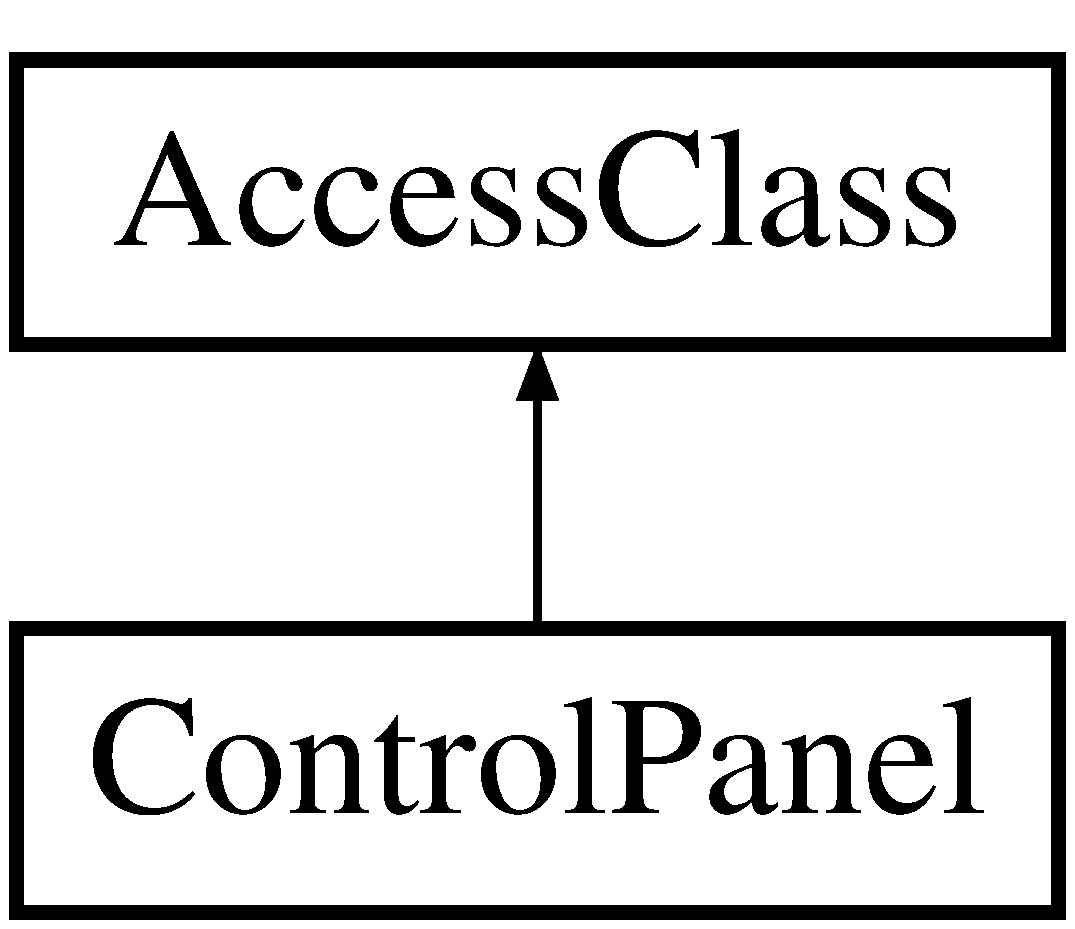
\includegraphics[height=2.000000cm]{classControlPanel}
\end{center}
\end{figure}
\subsection*{Public Member Functions}
\begin{DoxyCompactItemize}
\item 
\hypertarget{classControlPanel_a3d1860dbaa23c7c0b98b9f8caddaeef3}{{\bfseries Control\-Panel} (\hyperlink{classProcessorGraph}{Processor\-Graph} $\ast$graph, \hyperlink{classAudioComponent}{Audio\-Component} $\ast$audio)}\label{classControlPanel_a3d1860dbaa23c7c0b98b9f8caddaeef3}

\item 
\hypertarget{classControlPanel_a0e95cce1ecb861a21ae5aeb07a5c8820}{void {\bfseries disable\-Callbacks} ()}\label{classControlPanel_a0e95cce1ecb861a21ae5aeb07a5c8820}

\item 
\hypertarget{classControlPanel_a180e7c402f30514d8e4667afb61d5647}{\hyperlink{classAccessClass}{Access\-Class} $\ast$ {\bfseries get\-Audio\-Editor} ()}\label{classControlPanel_a180e7c402f30514d8e4667afb61d5647}

\item 
\hypertarget{classControlPanel_a79310ce5e86258dd74d4afcdb624a0ec}{void {\bfseries open\-State} (bool)}\label{classControlPanel_a79310ce5e86258dd74d4afcdb624a0ec}

\item 
\hypertarget{classControlPanel_a40df9a6291f6f8325db76e51cda37d63}{void {\bfseries toggle\-State} ()}\label{classControlPanel_a40df9a6291f6f8325db76e51cda37d63}

\item 
\hypertarget{classControlPanel_af5834f9032f88c6578b557cbd9e5f5eb}{bool {\bfseries is\-Open} ()}\label{classControlPanel_af5834f9032f88c6578b557cbd9e5f5eb}

\end{DoxyCompactItemize}
\subsection*{Private Member Functions}
\begin{DoxyCompactItemize}
\item 
\hypertarget{classControlPanel_ac6971b9a71d13685f444cb6bb1ca2334}{void {\bfseries paint} (Graphics \&g)}\label{classControlPanel_ac6971b9a71d13685f444cb6bb1ca2334}

\item 
\hypertarget{classControlPanel_a63ab3761114921ef049e50e598a159ae}{void {\bfseries resized} ()}\label{classControlPanel_a63ab3761114921ef049e50e598a159ae}

\item 
\hypertarget{classControlPanel_a9225b9ace95a2418b70473acbcd03641}{void {\bfseries button\-Clicked} (Button $\ast$button)}\label{classControlPanel_a9225b9ace95a2418b70473acbcd03641}

\item 
\hypertarget{classControlPanel_a342fb2fdbffe41c69197be84347bf57a}{void {\bfseries action\-Listener\-Callback} (const String \&msg)}\label{classControlPanel_a342fb2fdbffe41c69197be84347bf57a}

\item 
\hypertarget{classControlPanel_aa433a41f4ff41ed416b4e7a7198672ad}{void {\bfseries update\-Child\-Components} ()}\label{classControlPanel_aa433a41f4ff41ed416b4e7a7198672ad}

\item 
\hypertarget{classControlPanel_af8620f539537d65a921731392f3a12ff}{void {\bfseries timer\-Callback} ()}\label{classControlPanel_af8620f539537d65a921731392f3a12ff}

\item 
\hypertarget{classControlPanel_ade499872219cfc2d96d14489c306d55a}{bool {\bfseries key\-Pressed} (const Key\-Press \&key)}\label{classControlPanel_ade499872219cfc2d96d14489c306d55a}

\item 
\hypertarget{classControlPanel_aa3b90d1032c9688b161afb23c06df7cc}{void {\bfseries create\-Paths} ()}\label{classControlPanel_aa3b90d1032c9688b161afb23c06df7cc}

\end{DoxyCompactItemize}
\subsection*{Private Attributes}
\begin{DoxyCompactItemize}
\item 
\hypertarget{classControlPanel_a4b9a83ab762f1a58ab247957dc58af12}{\hyperlink{classPlayButton}{Play\-Button} $\ast$ {\bfseries play\-Button}}\label{classControlPanel_a4b9a83ab762f1a58ab247957dc58af12}

\item 
\hypertarget{classControlPanel_aedab407279cbe739c3790699d4a46dd0}{\hyperlink{classRecordButton}{Record\-Button} $\ast$ {\bfseries record\-Button}}\label{classControlPanel_aedab407279cbe739c3790699d4a46dd0}

\item 
\hypertarget{classControlPanel_aeebb097e70665b1b487c9e0737da9c34}{\hyperlink{classClock}{Clock} $\ast$ {\bfseries master\-Clock}}\label{classControlPanel_aeebb097e70665b1b487c9e0737da9c34}

\item 
\hypertarget{classControlPanel_a6a532ba0667e6b160caccdeede3c32a4}{\hyperlink{classCPUMeter}{C\-P\-U\-Meter} $\ast$ {\bfseries cpu\-Meter}}\label{classControlPanel_a6a532ba0667e6b160caccdeede3c32a4}

\item 
\hypertarget{classControlPanel_ac6f45060580dba90914049dd6c84e599}{\hyperlink{classDiskSpaceMeter}{Disk\-Space\-Meter} $\ast$ {\bfseries disk\-Meter}}\label{classControlPanel_ac6f45060580dba90914049dd6c84e599}

\item 
\hypertarget{classControlPanel_ad38ee9953ba8d4d3cbbbf418547ac805}{\hyperlink{classAudioComponent}{Audio\-Component} $\ast$ {\bfseries audio}}\label{classControlPanel_ad38ee9953ba8d4d3cbbbf418547ac805}

\item 
\hypertarget{classControlPanel_aee34c7466b14f0fe02623237c679cc96}{\hyperlink{classProcessorGraph}{Processor\-Graph} $\ast$ {\bfseries graph}}\label{classControlPanel_aee34c7466b14f0fe02623237c679cc96}

\item 
\hypertarget{classControlPanel_ae094b5ddde0916feaef4af9d9c2b7517}{\hyperlink{classAudioEditor}{Audio\-Editor} $\ast$ {\bfseries audio\-Editor}}\label{classControlPanel_ae094b5ddde0916feaef4af9d9c2b7517}

\item 
\hypertarget{classControlPanel_a41c64ea3f778a3779d1779c6acb1baec}{Filename\-Component $\ast$ {\bfseries filename\-Component}}\label{classControlPanel_a41c64ea3f778a3779d1779c6acb1baec}

\item 
\hypertarget{classControlPanel_a0c941210737d30067a5c336f024c1157}{\hyperlink{classUtilityButton}{Utility\-Button} $\ast$ {\bfseries new\-Directory\-Button}}\label{classControlPanel_a0c941210737d30067a5c336f024c1157}

\item 
\hypertarget{classControlPanel_ab78156dbcac19b328ddb20d3c72e794b}{\hyperlink{classControlPanelButton}{Control\-Panel\-Button} $\ast$ {\bfseries cpb}}\label{classControlPanel_ab78156dbcac19b328ddb20d3c72e794b}

\item 
\hypertarget{classControlPanel_ae3e88f26d3d9b0a6e5be976beec7c443}{Font {\bfseries font}}\label{classControlPanel_ae3e88f26d3d9b0a6e5be976beec7c443}

\item 
\hypertarget{classControlPanel_a99a8244df64a86e35339bd7b54735cfa}{bool {\bfseries open}}\label{classControlPanel_a99a8244df64a86e35339bd7b54735cfa}

\item 
\hypertarget{classControlPanel_ab83143533f9630969a42b620ce5ca1db}{Path {\bfseries p1}}\label{classControlPanel_ab83143533f9630969a42b620ce5ca1db}

\item 
\hypertarget{classControlPanel_aea112d4e9c4bea8f44cbab90c1544ef2}{Path {\bfseries p2}}\label{classControlPanel_aea112d4e9c4bea8f44cbab90c1544ef2}

\end{DoxyCompactItemize}


The documentation for this class was generated from the following file\-:\begin{DoxyCompactItemize}
\item 
U\-I/Control\-Panel.\-h\end{DoxyCompactItemize}

\hypertarget{classControlPanelButton}{\section{Control\-Panel\-Button Class Reference}
\label{classControlPanelButton}\index{Control\-Panel\-Button@{Control\-Panel\-Button}}
}
\subsection*{Public Member Functions}
\begin{DoxyCompactItemize}
\item 
\hypertarget{classControlPanelButton_aeeb4bd4128b5301ac902f5e1d3da1eea}{{\bfseries Control\-Panel\-Button} (\hyperlink{classControlPanel}{Control\-Panel} $\ast$cp\-\_\-)}\label{classControlPanelButton_aeeb4bd4128b5301ac902f5e1d3da1eea}

\item 
\hypertarget{classControlPanelButton_a49dd109b769582b9598a0f454fd39f06}{bool {\bfseries is\-Open} ()}\label{classControlPanelButton_a49dd109b769582b9598a0f454fd39f06}

\item 
\hypertarget{classControlPanelButton_a0158e881227f2382bdd3c71dada7f7f6}{void {\bfseries toggle\-State} ()}\label{classControlPanelButton_a0158e881227f2382bdd3c71dada7f7f6}

\item 
\hypertarget{classControlPanelButton_a84715321abda621693cec2bab8c283fe}{void {\bfseries new\-Open\-G\-L\-Context\-Created} ()}\label{classControlPanelButton_a84715321abda621693cec2bab8c283fe}

\item 
\hypertarget{classControlPanelButton_a9ea43519c7ca66fb9920625936564a9f}{void {\bfseries render\-Open\-G\-L} ()}\label{classControlPanelButton_a9ea43519c7ca66fb9920625936564a9f}

\item 
\hypertarget{classControlPanelButton_afdf353dfcec135b9150a3bda9e2da0e6}{void {\bfseries draw\-Button} ()}\label{classControlPanelButton_afdf353dfcec135b9150a3bda9e2da0e6}

\item 
\hypertarget{classControlPanelButton_a9b3041e05e6dcdb77020e78a3b0c2e26}{void {\bfseries mouse\-Down} (const Mouse\-Event \&e)}\label{classControlPanelButton_a9b3041e05e6dcdb77020e78a3b0c2e26}

\end{DoxyCompactItemize}
\subsection*{Private Attributes}
\begin{DoxyCompactItemize}
\item 
\hypertarget{classControlPanelButton_af324dcbcd32fdd7e7a1636ba8749f1c1}{\hyperlink{classControlPanel}{Control\-Panel} $\ast$ {\bfseries cp}}\label{classControlPanelButton_af324dcbcd32fdd7e7a1636ba8749f1c1}

\item 
\hypertarget{classControlPanelButton_a8963abee7f6d639bf0f192532d465f95}{bool {\bfseries open}}\label{classControlPanelButton_a8963abee7f6d639bf0f192532d465f95}

\end{DoxyCompactItemize}


The documentation for this class was generated from the following file\-:\begin{DoxyCompactItemize}
\item 
U\-I/Control\-Panel.\-h\end{DoxyCompactItemize}

\hypertarget{classCPUMeter}{\section{C\-P\-U\-Meter Class Reference}
\label{classCPUMeter}\index{C\-P\-U\-Meter@{C\-P\-U\-Meter}}
}
\subsection*{Public Member Functions}
\begin{DoxyCompactItemize}
\item 
\hypertarget{classCPUMeter_acec74e9f60516cd756c0f4a6e8cc7c60}{void {\bfseries update\-C\-P\-U} (float usage)}\label{classCPUMeter_acec74e9f60516cd756c0f4a6e8cc7c60}

\item 
\hypertarget{classCPUMeter_a010aa0a79b6ad5056ea7805266f36403}{void {\bfseries paint} (Graphics \&g)}\label{classCPUMeter_a010aa0a79b6ad5056ea7805266f36403}

\end{DoxyCompactItemize}
\subsection*{Private Attributes}
\begin{DoxyCompactItemize}
\item 
\hypertarget{classCPUMeter_a0f6d8aec5c432c61c8f7a1fe255967da}{Font {\bfseries font}}\label{classCPUMeter_a0f6d8aec5c432c61c8f7a1fe255967da}

\item 
\hypertarget{classCPUMeter_a630638ac674c7dbd9d29e058f5005fb5}{float {\bfseries cpu}}\label{classCPUMeter_a630638ac674c7dbd9d29e058f5005fb5}

\item 
\hypertarget{classCPUMeter_a8112f3d9893336aa9dbdc61050304e81}{float {\bfseries last\-Cpu}}\label{classCPUMeter_a8112f3d9893336aa9dbdc61050304e81}

\end{DoxyCompactItemize}


The documentation for this class was generated from the following file\-:\begin{DoxyCompactItemize}
\item 
U\-I/Control\-Panel.\-h\end{DoxyCompactItemize}

\hypertarget{classCustomLookAndFeel}{\section{Custom\-Look\-And\-Feel Class Reference}
\label{classCustomLookAndFeel}\index{Custom\-Look\-And\-Feel@{Custom\-Look\-And\-Feel}}
}


{\ttfamily \#include $<$Custom\-Look\-And\-Feel.\-h$>$}

\subsection*{Public Member Functions}
\begin{DoxyCompactItemize}
\item 
\hypertarget{classCustomLookAndFeel_a293de1ed51fc12098636c2bb62389a35}{void {\bfseries draw\-Tab\-Button} (Graphics \&g, int w, int h, const Colour \&preferred\-Colour, int tab\-Index, const String \&text, Button \&button, Tabbed\-Button\-Bar\-::\-Orientation, bool is\-Mouse\-Over, bool is\-Mouse\-Down, bool is\-Front\-Tab)}\label{classCustomLookAndFeel_a293de1ed51fc12098636c2bb62389a35}

\item 
\hypertarget{classCustomLookAndFeel_a10e1f39538e5ec8195adf49336fabdc1}{void {\bfseries draw\-Tab\-Button\-Text} (Graphics \&g, int x, int y, int w, int h, const Colour \&preferred\-Background\-Colour, int tab\-Index, const String \&text, Button \&button, Tabbed\-Button\-Bar\-::\-Orientation o, bool is\-Mouse\-Over, bool is\-Mouse\-Down, bool is\-Front\-Tab)}\label{classCustomLookAndFeel_a10e1f39538e5ec8195adf49336fabdc1}

\item 
\hypertarget{classCustomLookAndFeel_a087db189b43e809b93c3004850563157}{int {\bfseries get\-Tab\-Button\-Best\-Width} (int tab\-Index, const String \&text, int tab\-Depth, Button \&button)}\label{classCustomLookAndFeel_a087db189b43e809b93c3004850563157}

\item 
\hypertarget{classCustomLookAndFeel_a1d6fa4575f68909fae463bb1b5f55348}{int {\bfseries get\-Tab\-Button\-Space\-Around\-Image} ()}\label{classCustomLookAndFeel_a1d6fa4575f68909fae463bb1b5f55348}

\item 
\hypertarget{classCustomLookAndFeel_a0dcd1ad0afb18c7cfc72e5c33cc1b27e}{void {\bfseries draw\-Tab\-Area\-Behind\-Front\-Button} (Graphics \&g, int w, int h, Tabbed\-Button\-Bar \&tab\-Bar, Tabbed\-Button\-Bar\-::\-Orientation o)}\label{classCustomLookAndFeel_a0dcd1ad0afb18c7cfc72e5c33cc1b27e}

\item 
\hypertarget{classCustomLookAndFeel_a1d8165c009dc226434f73a6b90444c5e}{int {\bfseries get\-Tab\-Button\-Overlap} (int tab\-Depth)}\label{classCustomLookAndFeel_a1d8165c009dc226434f73a6b90444c5e}

\item 
\hypertarget{classCustomLookAndFeel_a6a725a762f4a681385b0dc28998a2c87}{void {\bfseries draw\-Scrollbar\-Button} (Graphics \&g, Scroll\-Bar \&scrollbar, int width, int height, int button\-Direction, bool is\-Scroll\-Bar\-Vertical, bool is\-Mouse\-Over\-Button, bool is\-Button\-Down)}\label{classCustomLookAndFeel_a6a725a762f4a681385b0dc28998a2c87}

\item 
\hypertarget{classCustomLookAndFeel_a264ec5aef0a2c35ab5cdb46c086fd756}{void {\bfseries draw\-Scrollbar} (Graphics \&g, Scroll\-Bar \&scrollbar, int x, int y, int width, int height, bool is\-Scrollbar\-Vertical, int thumb\-Start\-Position, int thumb\-Size, bool is\-Mouse\-Over, bool is\-Mouse\-Down)}\label{classCustomLookAndFeel_a264ec5aef0a2c35ab5cdb46c086fd756}

\item 
\hypertarget{classCustomLookAndFeel_a36c450599faf6763631bad3469bc697e}{void {\bfseries draw\-Linear\-Slider\-Thumb} (Graphics \&g, int x, int y, int width, int height, float slider\-Pos, float min\-Slider\-Pos, float max\-Slider\-Pos, const Slider\-::\-Slider\-Style style, Slider \&slider)}\label{classCustomLookAndFeel_a36c450599faf6763631bad3469bc697e}

\item 
\hypertarget{classCustomLookAndFeel_a21a063ecef1bf98e3b63443dafdc2a6b}{void {\bfseries draw\-Linear\-Slider\-Background} (Graphics \&g, int x, int y, int width, int height, float, float, float, const Slider\-::\-Slider\-Style, Slider \&slider)}\label{classCustomLookAndFeel_a21a063ecef1bf98e3b63443dafdc2a6b}

\item 
\hypertarget{classCustomLookAndFeel_aa19bb222a239cdf0c749d478780356fd}{int {\bfseries get\-Slider\-Thumb\-Radius} (Slider \&slider)}\label{classCustomLookAndFeel_aa19bb222a239cdf0c749d478780356fd}

\item 
\hypertarget{classCustomLookAndFeel_aa88e40058d027736cbbacdd55a6127fc}{void {\bfseries draw\-Slider\-Knob} (Graphics \&g, const float x, const float y, const float diameter, const Colour \&colour, const float outline\-Thickness)  throw ()}\label{classCustomLookAndFeel_aa88e40058d027736cbbacdd55a6127fc}

\item 
\hypertarget{classCustomLookAndFeel_a90629a459f908cc6e26ecaa20be9d261}{void {\bfseries draw\-Glass\-Pointer} (Graphics \&g, const float x, const float y, const float diameter, const Colour \&colour, const float outline\-Thickness, const int direction)  throw ()}\label{classCustomLookAndFeel_a90629a459f908cc6e26ecaa20be9d261}

\item 
\hypertarget{classCustomLookAndFeel_af317608dd49be6e510c287ece03f425a}{void {\bfseries draw\-Combo\-Box} (Graphics \&g, int width, int height, const bool is\-Button\-Down, int button\-X, int button\-Y, int button\-W, int button\-H, Combo\-Box \&box)}\label{classCustomLookAndFeel_af317608dd49be6e510c287ece03f425a}

\end{DoxyCompactItemize}
\subsection*{Public Attributes}
\begin{DoxyCompactItemize}
\item 
\hypertarget{classCustomLookAndFeel_aa04bd6a6419986c7aadb62baaca294a3}{Typeface\-::\-Ptr {\bfseries Miso}}\label{classCustomLookAndFeel_aa04bd6a6419986c7aadb62baaca294a3}

\end{DoxyCompactItemize}


\subsection{Detailed Description}
Used to modify the appearance of the application.

Currently contains methods for drawing custom tabs, custom scroll bars, and custom sliders.

\begin{DoxySeeAlso}{See also}
\hyperlink{classMainWindow}{Main\-Window} 
\end{DoxySeeAlso}


The documentation for this class was generated from the following file\-:\begin{DoxyCompactItemize}
\item 
U\-I/Custom\-Look\-And\-Feel.\-h\end{DoxyCompactItemize}

\hypertarget{classDataBuffer}{\section{Data\-Buffer Class Reference}
\label{classDataBuffer}\index{Data\-Buffer@{Data\-Buffer}}
}
\subsection*{Public Member Functions}
\begin{DoxyCompactItemize}
\item 
\hypertarget{classDataBuffer_a05ce6a6b3a4be03dbe2ec15173a51c7c}{{\bfseries Data\-Buffer} (int chans, int size)}\label{classDataBuffer_a05ce6a6b3a4be03dbe2ec15173a51c7c}

\item 
\hypertarget{classDataBuffer_ac114fa2ba9b9ad0545b6f846dc098c21}{void {\bfseries clear} ()}\label{classDataBuffer_ac114fa2ba9b9ad0545b6f846dc098c21}

\item 
\hypertarget{classDataBuffer_a5cc06461e64712fbc015dcab84de51e3}{void {\bfseries add\-To\-Buffer} (float $\ast$data, int num\-Items)}\label{classDataBuffer_a5cc06461e64712fbc015dcab84de51e3}

\item 
\hypertarget{classDataBuffer_a7594cd0003317cb88e732215ba664c58}{int {\bfseries get\-Num\-Samples} ()}\label{classDataBuffer_a7594cd0003317cb88e732215ba664c58}

\item 
\hypertarget{classDataBuffer_ad2e746f7588cf608580f9b652bdf8bf7}{int {\bfseries read\-All\-From\-Buffer} (Audio\-Sample\-Buffer \&data, int max\-Size)}\label{classDataBuffer_ad2e746f7588cf608580f9b652bdf8bf7}

\end{DoxyCompactItemize}
\subsection*{Private Member Functions}
\begin{DoxyCompactItemize}
\item 
\hypertarget{classDataBuffer_aedd1c980c44c5f353cf4fcc1653ca9eb}{{\bfseries J\-U\-C\-E\-\_\-\-D\-E\-C\-L\-A\-R\-E\-\_\-\-N\-O\-N\-\_\-\-C\-O\-P\-Y\-A\-B\-L\-E\-\_\-\-W\-I\-T\-H\-\_\-\-L\-E\-A\-K\-\_\-\-D\-E\-T\-E\-C\-T\-O\-R} (\hyperlink{classDataBuffer}{Data\-Buffer})}\label{classDataBuffer_aedd1c980c44c5f353cf4fcc1653ca9eb}

\end{DoxyCompactItemize}
\subsection*{Private Attributes}
\begin{DoxyCompactItemize}
\item 
\hypertarget{classDataBuffer_a5961ca39f034fa05de297d35b6bb58ce}{Abstract\-Fifo {\bfseries abstract\-Fifo}}\label{classDataBuffer_a5961ca39f034fa05de297d35b6bb58ce}

\item 
\hypertarget{classDataBuffer_a8d1728e754f571361f9dca6d30f610ca}{Audio\-Sample\-Buffer {\bfseries buffer}}\label{classDataBuffer_a8d1728e754f571361f9dca6d30f610ca}

\item 
\hypertarget{classDataBuffer_aa58c07ffde819061664ca94562604f14}{int {\bfseries num\-Chans}}\label{classDataBuffer_aa58c07ffde819061664ca94562604f14}

\end{DoxyCompactItemize}


The documentation for this class was generated from the following file\-:\begin{DoxyCompactItemize}
\item 
Processors/\-Data\-Threads/Data\-Buffer.\-h\end{DoxyCompactItemize}

\hypertarget{classDataThread}{\section{Data\-Thread Class Reference}
\label{classDataThread}\index{Data\-Thread@{Data\-Thread}}
}
Inheritance diagram for Data\-Thread\-:\begin{figure}[H]
\begin{center}
\leavevmode
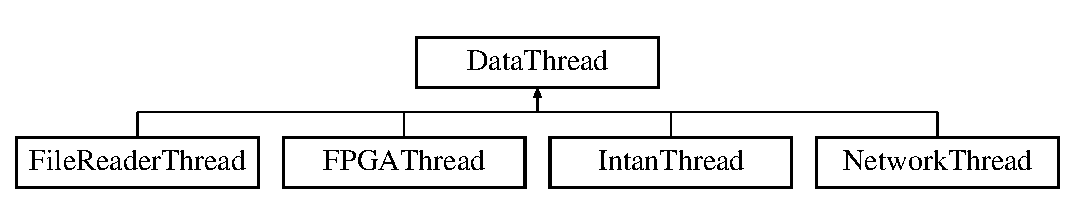
\includegraphics[height=2.000000cm]{classDataThread}
\end{center}
\end{figure}
\subsection*{Public Member Functions}
\begin{DoxyCompactItemize}
\item 
\hypertarget{classDataThread_acb6f10d03646d7c2faff5c7e3bc1a5e7}{{\bfseries Data\-Thread} (\hyperlink{classSourceNode}{Source\-Node} $\ast$sn)}\label{classDataThread_acb6f10d03646d7c2faff5c7e3bc1a5e7}

\item 
\hypertarget{classDataThread_ae1d41cdc6b7fbd8160e18c3cf1812471}{void {\bfseries run} ()}\label{classDataThread_ae1d41cdc6b7fbd8160e18c3cf1812471}

\item 
\hypertarget{classDataThread_aba376e486bef12a53c588f65e20d7978}{\hyperlink{classDataBuffer}{Data\-Buffer} $\ast$ {\bfseries get\-Buffer\-Address} ()}\label{classDataThread_aba376e486bef12a53c588f65e20d7978}

\item 
\hypertarget{classDataThread_adbd6623e8892aad3c5f5588aff3ff195}{virtual bool {\bfseries update\-Buffer} ()=0}\label{classDataThread_adbd6623e8892aad3c5f5588aff3ff195}

\item 
\hypertarget{classDataThread_af62fa85b1ac69f1f3b3f53150bf55f23}{virtual bool {\bfseries found\-Input\-Source} ()=0}\label{classDataThread_af62fa85b1ac69f1f3b3f53150bf55f23}

\item 
\hypertarget{classDataThread_a0ff3b07535413c15cc515bd65b2ce2b8}{virtual bool {\bfseries start\-Acquisition} ()=0}\label{classDataThread_a0ff3b07535413c15cc515bd65b2ce2b8}

\item 
\hypertarget{classDataThread_a81cbc75ecf5ddb83d64d56da13b10a29}{virtual bool {\bfseries stop\-Acquisition} ()=0}\label{classDataThread_a81cbc75ecf5ddb83d64d56da13b10a29}

\item 
\hypertarget{classDataThread_a2eb3af064cfe39d83dc19dd6e4f5de06}{virtual int {\bfseries get\-Num\-Channels} ()=0}\label{classDataThread_a2eb3af064cfe39d83dc19dd6e4f5de06}

\item 
\hypertarget{classDataThread_a86f12c1b334ae8c4cd39c493cc123302}{virtual float {\bfseries get\-Sample\-Rate} ()=0}\label{classDataThread_a86f12c1b334ae8c4cd39c493cc123302}

\item 
\hypertarget{classDataThread_a679d8b6d9c25dba87cdf8b248eb96d4c}{virtual float {\bfseries get\-Bit\-Volts} ()=0}\label{classDataThread_a679d8b6d9c25dba87cdf8b248eb96d4c}

\end{DoxyCompactItemize}
\subsection*{Public Attributes}
\begin{DoxyCompactItemize}
\item 
\hypertarget{classDataThread_a70d6a9b3496ef57ce2b55a4af6ee8de5}{Scoped\-Pointer$<$ \hyperlink{classDataBuffer}{Data\-Buffer} $>$ {\bfseries data\-Buffer}}\label{classDataThread_a70d6a9b3496ef57ce2b55a4af6ee8de5}

\item 
\hypertarget{classDataThread_a6a26fc244b2ce396c5c013353fb6293e}{\hyperlink{classSourceNode}{Source\-Node} $\ast$ {\bfseries sn}}\label{classDataThread_a6a26fc244b2ce396c5c013353fb6293e}

\end{DoxyCompactItemize}
\subsection*{Private Member Functions}
\begin{DoxyCompactItemize}
\item 
\hypertarget{classDataThread_a86d08fbb9f2ee6534129671959f5de6d}{{\bfseries J\-U\-C\-E\-\_\-\-D\-E\-C\-L\-A\-R\-E\-\_\-\-N\-O\-N\-\_\-\-C\-O\-P\-Y\-A\-B\-L\-E\-\_\-\-W\-I\-T\-H\-\_\-\-L\-E\-A\-K\-\_\-\-D\-E\-T\-E\-C\-T\-O\-R} (\hyperlink{classDataThread}{Data\-Thread})}\label{classDataThread_a86d08fbb9f2ee6534129671959f5de6d}

\end{DoxyCompactItemize}


The documentation for this class was generated from the following file\-:\begin{DoxyCompactItemize}
\item 
Processors/\-Data\-Threads/Data\-Thread.\-h\end{DoxyCompactItemize}

\hypertarget{classDataViewport}{\section{Data\-Viewport Class Reference}
\label{classDataViewport}\index{Data\-Viewport@{Data\-Viewport}}
}
Inheritance diagram for Data\-Viewport\-:\begin{figure}[H]
\begin{center}
\leavevmode
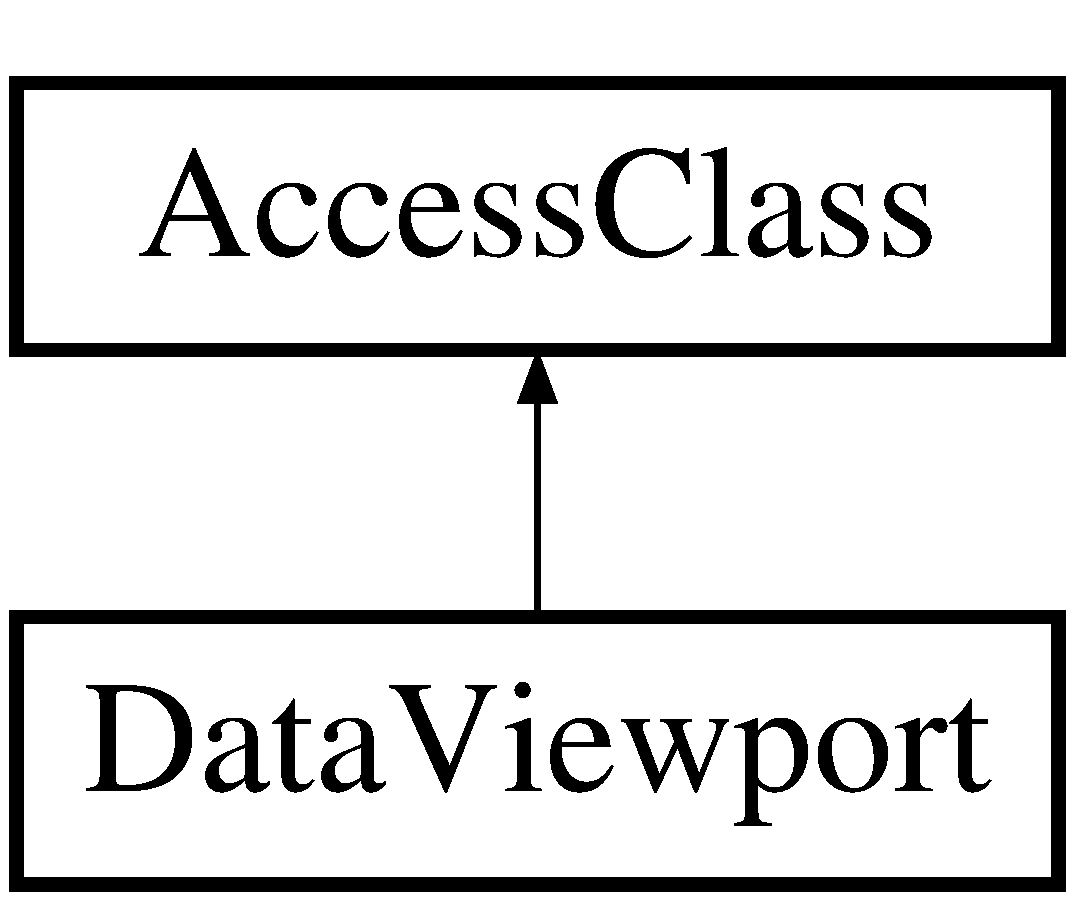
\includegraphics[height=2.000000cm]{classDataViewport}
\end{center}
\end{figure}
\subsection*{Public Member Functions}
\begin{DoxyCompactItemize}
\item 
int \hyperlink{classDataViewport_accdcf7187ec5864fdbf0c2a3e605b072}{add\-Tab\-To\-Data\-Viewport} (String tab\-Name, Component $\ast$component\-To\-Add, \hyperlink{classGenericEditor}{Generic\-Editor} $\ast$editor)
\item 
void \hyperlink{classDataViewport_ad68668771aa73c3cdcefcfa692fe0098}{destroy\-Tab} (int)
\item 
void \hyperlink{classDataViewport_a03221f79ac5f5edd473221bfc8f42dcc}{select\-Tab} (int)
\item 
void \hyperlink{classDataViewport_a3d468d1c0f59f84165be4b68c0882c8d}{current\-Tab\-Changed} (int new\-Index, const String \&new\-Tab\-Name)
\item 
void \hyperlink{classDataViewport_a6f501d921cd1b2539790624accc6ea00}{disable\-Connection\-To\-Editor\-Viewport} ()
\end{DoxyCompactItemize}
\subsection*{Private Member Functions}
\begin{DoxyCompactItemize}
\item 
\hypertarget{classDataViewport_a0edb05653624ca748aa2fb99be4a92d1}{void {\bfseries paint} (Graphics \&g)}\label{classDataViewport_a0edb05653624ca748aa2fb99be4a92d1}

\item 
\hypertarget{classDataViewport_ade8ef66cda0ef16c1e8bac8acb0bb6f5}{{\bfseries J\-U\-C\-E\-\_\-\-D\-E\-C\-L\-A\-R\-E\-\_\-\-N\-O\-N\-\_\-\-C\-O\-P\-Y\-A\-B\-L\-E\-\_\-\-W\-I\-T\-H\-\_\-\-L\-E\-A\-K\-\_\-\-D\-E\-T\-E\-C\-T\-O\-R} (\hyperlink{classDataViewport}{Data\-Viewport})}\label{classDataViewport_ade8ef66cda0ef16c1e8bac8acb0bb6f5}

\end{DoxyCompactItemize}
\subsection*{Private Attributes}
\begin{DoxyCompactItemize}
\item 
\hypertarget{classDataViewport_aed6c8f52223b4a0f18522b5d955ebb78}{Array$<$ int $>$ {\bfseries tab\-Array}}\label{classDataViewport_aed6c8f52223b4a0f18522b5d955ebb78}

\item 
\hypertarget{classDataViewport_af20639966e4c4ac17eeaf2ff76fb4067}{Array$<$ \hyperlink{classGenericEditor}{Generic\-Editor} $\ast$ $>$ {\bfseries editor\-Array}}\label{classDataViewport_af20639966e4c4ac17eeaf2ff76fb4067}

\item 
\hypertarget{classDataViewport_a1ede587e57426d557975837ecef551f4}{int {\bfseries tab\-Depth}}\label{classDataViewport_a1ede587e57426d557975837ecef551f4}

\item 
\hypertarget{classDataViewport_a5e55f6f3324b280f3e26993b52ba3192}{bool {\bfseries shutdown}}\label{classDataViewport_a5e55f6f3324b280f3e26993b52ba3192}

\end{DoxyCompactItemize}


\subsection{Member Function Documentation}
\hypertarget{classDataViewport_accdcf7187ec5864fdbf0c2a3e605b072}{\index{Data\-Viewport@{Data\-Viewport}!add\-Tab\-To\-Data\-Viewport@{add\-Tab\-To\-Data\-Viewport}}
\index{add\-Tab\-To\-Data\-Viewport@{add\-Tab\-To\-Data\-Viewport}!DataViewport@{Data\-Viewport}}
\subsubsection[{add\-Tab\-To\-Data\-Viewport}]{\setlength{\rightskip}{0pt plus 5cm}int Data\-Viewport\-::add\-Tab\-To\-Data\-Viewport (
\begin{DoxyParamCaption}
\item[{String}]{tab\-Name, }
\item[{Component $\ast$}]{component\-To\-Add, }
\item[{{\bf Generic\-Editor} $\ast$}]{editor}
\end{DoxyParamCaption}
)}}\label{classDataViewport_accdcf7187ec5864fdbf0c2a3e605b072}
Adds a new tab and returns the tab index. \hypertarget{classDataViewport_a3d468d1c0f59f84165be4b68c0882c8d}{\index{Data\-Viewport@{Data\-Viewport}!current\-Tab\-Changed@{current\-Tab\-Changed}}
\index{current\-Tab\-Changed@{current\-Tab\-Changed}!DataViewport@{Data\-Viewport}}
\subsubsection[{current\-Tab\-Changed}]{\setlength{\rightskip}{0pt plus 5cm}void Data\-Viewport\-::current\-Tab\-Changed (
\begin{DoxyParamCaption}
\item[{int}]{new\-Index, }
\item[{const String \&}]{new\-Tab\-Name}
\end{DoxyParamCaption}
)}}\label{classDataViewport_a3d468d1c0f59f84165be4b68c0882c8d}
Informs the component of the current tab that it's now active. \hypertarget{classDataViewport_ad68668771aa73c3cdcefcfa692fe0098}{\index{Data\-Viewport@{Data\-Viewport}!destroy\-Tab@{destroy\-Tab}}
\index{destroy\-Tab@{destroy\-Tab}!DataViewport@{Data\-Viewport}}
\subsubsection[{destroy\-Tab}]{\setlength{\rightskip}{0pt plus 5cm}void Data\-Viewport\-::destroy\-Tab (
\begin{DoxyParamCaption}
\item[{int}]{}
\end{DoxyParamCaption}
)}}\label{classDataViewport_ad68668771aa73c3cdcefcfa692fe0098}
Removes a tab with a specified index. \hypertarget{classDataViewport_a6f501d921cd1b2539790624accc6ea00}{\index{Data\-Viewport@{Data\-Viewport}!disable\-Connection\-To\-Editor\-Viewport@{disable\-Connection\-To\-Editor\-Viewport}}
\index{disable\-Connection\-To\-Editor\-Viewport@{disable\-Connection\-To\-Editor\-Viewport}!DataViewport@{Data\-Viewport}}
\subsubsection[{disable\-Connection\-To\-Editor\-Viewport}]{\setlength{\rightskip}{0pt plus 5cm}void Data\-Viewport\-::disable\-Connection\-To\-Editor\-Viewport (
\begin{DoxyParamCaption}
{}
\end{DoxyParamCaption}
)}}\label{classDataViewport_a6f501d921cd1b2539790624accc6ea00}
Prevent \hyperlink{classDataViewport}{Data\-Viewport} from signaling \hyperlink{classEditorViewport}{Editor\-Viewport} when changing tabs. \hypertarget{classDataViewport_a03221f79ac5f5edd473221bfc8f42dcc}{\index{Data\-Viewport@{Data\-Viewport}!select\-Tab@{select\-Tab}}
\index{select\-Tab@{select\-Tab}!DataViewport@{Data\-Viewport}}
\subsubsection[{select\-Tab}]{\setlength{\rightskip}{0pt plus 5cm}void Data\-Viewport\-::select\-Tab (
\begin{DoxyParamCaption}
\item[{int}]{}
\end{DoxyParamCaption}
)}}\label{classDataViewport_a03221f79ac5f5edd473221bfc8f42dcc}
Select a tab with a specified index. 

The documentation for this class was generated from the following file\-:\begin{DoxyCompactItemize}
\item 
U\-I/Data\-Viewport.\-h\end{DoxyCompactItemize}

\hypertarget{classDataWindow}{\section{Data\-Window Class Reference}
\label{classDataWindow}\index{Data\-Window@{Data\-Window}}
}


{\ttfamily \#include $<$Data\-Window.\-h$>$}

\subsection*{Public Member Functions}
\begin{DoxyCompactItemize}
\item 
\hypertarget{classDataWindow_a2c1a0313c6a13ebf16c40db1a5832cca}{{\bfseries Data\-Window} (Button $\ast$button)}\label{classDataWindow_a2c1a0313c6a13ebf16c40db1a5832cca}

\item 
\hypertarget{classDataWindow_ad3e0318d8e542aa12b30791441cae5ab}{void {\bfseries close\-Button\-Pressed} ()}\label{classDataWindow_ad3e0318d8e542aa12b30791441cae5ab}

\end{DoxyCompactItemize}
\subsection*{Private Member Functions}
\begin{DoxyCompactItemize}
\item 
\hypertarget{classDataWindow_a4e4c8bb6b88c32202f4ee263aef5cbf5}{{\bfseries J\-U\-C\-E\-\_\-\-D\-E\-C\-L\-A\-R\-E\-\_\-\-N\-O\-N\-\_\-\-C\-O\-P\-Y\-A\-B\-L\-E\-\_\-\-W\-I\-T\-H\-\_\-\-L\-E\-A\-K\-\_\-\-D\-E\-T\-E\-C\-T\-O\-R} (\hyperlink{classDataWindow}{Data\-Window})}\label{classDataWindow_a4e4c8bb6b88c32202f4ee263aef5cbf5}

\end{DoxyCompactItemize}
\subsection*{Private Attributes}
\begin{DoxyCompactItemize}
\item 
\hypertarget{classDataWindow_a561ef07ade52eb60a50a13c1c6fc1622}{Button $\ast$ {\bfseries control\-Button}}\label{classDataWindow_a561ef07ade52eb60a50a13c1c6fc1622}

\end{DoxyCompactItemize}


\subsection{Detailed Description}
Allows Open\-G\-L visualizers to be placed in their own window.

\begin{DoxySeeAlso}{See also}
\hyperlink{classDataViewport}{Data\-Viewport}, \hyperlink{classOpenGLCanvas}{Open\-G\-L\-Canvas} 
\end{DoxySeeAlso}


The documentation for this class was generated from the following file\-:\begin{DoxyCompactItemize}
\item 
Processors/\-Visualization/Data\-Window.\-h\end{DoxyCompactItemize}

\hypertarget{classDiskSpaceMeter}{\section{Disk\-Space\-Meter Class Reference}
\label{classDiskSpaceMeter}\index{Disk\-Space\-Meter@{Disk\-Space\-Meter}}
}
\subsection*{Public Member Functions}
\begin{DoxyCompactItemize}
\item 
\hypertarget{classDiskSpaceMeter_acc3483e3a49b12a9c5dd13568c98aeec}{void {\bfseries update\-Disk\-Space} (float percent)}\label{classDiskSpaceMeter_acc3483e3a49b12a9c5dd13568c98aeec}

\item 
\hypertarget{classDiskSpaceMeter_a11df895ab492661e07e3b6c4393c75b2}{void {\bfseries paint} (Graphics \&g)}\label{classDiskSpaceMeter_a11df895ab492661e07e3b6c4393c75b2}

\end{DoxyCompactItemize}
\subsection*{Private Attributes}
\begin{DoxyCompactItemize}
\item 
\hypertarget{classDiskSpaceMeter_a8f740abddda096f2d51f289f2bf995af}{Font {\bfseries font}}\label{classDiskSpaceMeter_a8f740abddda096f2d51f289f2bf995af}

\item 
\hypertarget{classDiskSpaceMeter_a1174c651208caa6c7528a948cb4b4514}{float {\bfseries disk\-Free}}\label{classDiskSpaceMeter_a1174c651208caa6c7528a948cb4b4514}

\item 
\hypertarget{classDiskSpaceMeter_aa0cfc8c37918982d8ddee518e91d7565}{\hyperlink{classProcessorGraph}{Processor\-Graph} $\ast$ {\bfseries graph}}\label{classDiskSpaceMeter_aa0cfc8c37918982d8ddee518e91d7565}

\end{DoxyCompactItemize}


The documentation for this class was generated from the following file\-:\begin{DoxyCompactItemize}
\item 
U\-I/Control\-Panel.\-h\end{DoxyCompactItemize}

\hypertarget{classDrawerButton}{\section{Drawer\-Button Class Reference}
\label{classDrawerButton}\index{Drawer\-Button@{Drawer\-Button}}
}
\subsection*{Public Member Functions}
\begin{DoxyCompactItemize}
\item 
\hypertarget{classDrawerButton_a152c65b0b22c997a9424f5d45bbdabc3}{{\bfseries Drawer\-Button} (const String \&name)}\label{classDrawerButton_a152c65b0b22c997a9424f5d45bbdabc3}

\end{DoxyCompactItemize}
\subsection*{Private Member Functions}
\begin{DoxyCompactItemize}
\item 
\hypertarget{classDrawerButton_a94263ddea088b6c16793d79682df6c40}{void {\bfseries paint\-Button} (Graphics \&g, bool is\-Mouse\-Over, bool is\-Button\-Down)}\label{classDrawerButton_a94263ddea088b6c16793d79682df6c40}

\end{DoxyCompactItemize}


The documentation for this class was generated from the following file\-:\begin{DoxyCompactItemize}
\item 
Processors/\-Editors/Generic\-Editor.\-h\end{DoxyCompactItemize}

\hypertarget{classEditorButton}{\section{Editor\-Button Class Reference}
\label{classEditorButton}\index{Editor\-Button@{Editor\-Button}}
}
\subsection*{Public Member Functions}
\begin{DoxyCompactItemize}
\item 
\hypertarget{classEditorButton_a35ec700d47c757da0bf5f2bd29103ade}{{\bfseries Editor\-Button} (const String \&name, Font \&f)}\label{classEditorButton_a35ec700d47c757da0bf5f2bd29103ade}

\item 
\hypertarget{classEditorButton_a59b8c7d8aaecbf1284dd0984ea38db1e}{bool {\bfseries get\-State} ()}\label{classEditorButton_a59b8c7d8aaecbf1284dd0984ea38db1e}

\item 
\hypertarget{classEditorButton_a214cdec9d7b55f60c1bcbf1ba9c66067}{void {\bfseries set\-State} (bool state)}\label{classEditorButton_a214cdec9d7b55f60c1bcbf1ba9c66067}

\end{DoxyCompactItemize}
\subsection*{Private Member Functions}
\begin{DoxyCompactItemize}
\item 
\hypertarget{classEditorButton_a1c1cdda922d62e682dce7389372a8ba4}{void {\bfseries paint\-Button} (Graphics \&g, bool is\-Mouse\-Over, bool is\-Button\-Down)}\label{classEditorButton_a1c1cdda922d62e682dce7389372a8ba4}

\item 
\hypertarget{classEditorButton_a6e3c89fb005ae8a45282730781504afe}{void {\bfseries resized} ()}\label{classEditorButton_a6e3c89fb005ae8a45282730781504afe}

\end{DoxyCompactItemize}
\subsection*{Private Attributes}
\begin{DoxyCompactItemize}
\item 
\hypertarget{classEditorButton_a0aa12206f7c62b11345765bb13f6c79a}{Path {\bfseries outline\-Path}}\label{classEditorButton_a0aa12206f7c62b11345765bb13f6c79a}

\item 
\hypertarget{classEditorButton_ab304ddf5eae1493122cbff94c1f1ef38}{int {\bfseries type}}\label{classEditorButton_ab304ddf5eae1493122cbff94c1f1ef38}

\item 
\hypertarget{classEditorButton_a17ede639862a8ba98c2f9b5db2a4c315}{Font {\bfseries button\-Font}}\label{classEditorButton_a17ede639862a8ba98c2f9b5db2a4c315}

\item 
\hypertarget{classEditorButton_a48df6c37c0b8b56340b6488e487f43db}{bool {\bfseries is\-Enabled}}\label{classEditorButton_a48df6c37c0b8b56340b6488e487f43db}

\item 
\hypertarget{classEditorButton_a18ab69b4c86f0bb5e4b87f41964503e3}{Colour\-Gradient {\bfseries selected\-Grad}}\label{classEditorButton_a18ab69b4c86f0bb5e4b87f41964503e3}

\item 
\hypertarget{classEditorButton_afc3411c019d5befd3ca2fb694e16ccf8}{Colour\-Gradient {\bfseries selected\-Over\-Grad}}\label{classEditorButton_afc3411c019d5befd3ca2fb694e16ccf8}

\item 
\hypertarget{classEditorButton_a152e8a9731e6860395fc8c0b7bcd60af}{Colour\-Gradient {\bfseries neutral\-Grad}}\label{classEditorButton_a152e8a9731e6860395fc8c0b7bcd60af}

\item 
\hypertarget{classEditorButton_a1090cad0c5a5794618240b0756857025}{Colour\-Gradient {\bfseries neutral\-Over\-Grad}}\label{classEditorButton_a1090cad0c5a5794618240b0756857025}

\end{DoxyCompactItemize}


The documentation for this class was generated from the following file\-:\begin{DoxyCompactItemize}
\item 
Processors/\-Editors/Channel\-Selector.\-h\end{DoxyCompactItemize}

\hypertarget{classEditorScrollButton}{\section{Editor\-Scroll\-Button Class Reference}
\label{classEditorScrollButton}\index{Editor\-Scroll\-Button@{Editor\-Scroll\-Button}}
}


{\ttfamily \#include $<$Editor\-Viewport\-Buttons.\-h$>$}

\subsection*{Public Types}
\begin{DoxyCompactItemize}
\item 
enum {\bfseries type} \{ {\bfseries L\-E\-F\-T}, 
{\bfseries R\-I\-G\-H\-T}
 \}
\end{DoxyCompactItemize}
\subsection*{Public Member Functions}
\begin{DoxyCompactItemize}
\item 
\hypertarget{classEditorScrollButton_a5fb520c9d69a64445237b4460f5f3996}{{\bfseries Editor\-Scroll\-Button} (int type)}\label{classEditorScrollButton_a5fb520c9d69a64445237b4460f5f3996}

\item 
\hypertarget{classEditorScrollButton_afa1c06306541020c5357ca73b0e5afe7}{void {\bfseries set\-Active} (bool)}\label{classEditorScrollButton_afa1c06306541020c5357ca73b0e5afe7}

\end{DoxyCompactItemize}
\subsection*{Public Attributes}
\begin{DoxyCompactItemize}
\item 
\hypertarget{classEditorScrollButton_a1849b6801a59f08c82dfeea8be6ddd59}{bool {\bfseries is\-Active}}\label{classEditorScrollButton_a1849b6801a59f08c82dfeea8be6ddd59}

\item 
\hypertarget{classEditorScrollButton_a2002c2eb1cbb326e41b9092717b5184f}{int {\bfseries direction}}\label{classEditorScrollButton_a2002c2eb1cbb326e41b9092717b5184f}

\item 
\hypertarget{classEditorScrollButton_a961f0d5da5a2c40568f9dd1b5956337f}{Drawable\-Path {\bfseries inactive}}\label{classEditorScrollButton_a961f0d5da5a2c40568f9dd1b5956337f}

\item 
\hypertarget{classEditorScrollButton_ac5fdca798bd5d884be05b2ff30cb2987}{Drawable\-Path {\bfseries active\-Normal}}\label{classEditorScrollButton_ac5fdca798bd5d884be05b2ff30cb2987}

\item 
\hypertarget{classEditorScrollButton_a40afae70addff0710126829c90cc5b5b}{Drawable\-Path {\bfseries active\-Over}}\label{classEditorScrollButton_a40afae70addff0710126829c90cc5b5b}

\item 
\hypertarget{classEditorScrollButton_a52bdfa45eede31bc1375601a6c586bb9}{Drawable\-Path {\bfseries active\-Down}}\label{classEditorScrollButton_a52bdfa45eede31bc1375601a6c586bb9}

\end{DoxyCompactItemize}


\subsection{Detailed Description}
A set of buttons for scrolling through editors and signal chains.

\begin{DoxySeeAlso}{See also}
\hyperlink{classEditorViewport}{Editor\-Viewport}. 
\end{DoxySeeAlso}


The documentation for this class was generated from the following file\-:\begin{DoxyCompactItemize}
\item 
U\-I/Editor\-Viewport\-Buttons.\-h\end{DoxyCompactItemize}

\hypertarget{classEditorViewport}{\section{Editor\-Viewport Class Reference}
\label{classEditorViewport}\index{Editor\-Viewport@{Editor\-Viewport}}
}
Inheritance diagram for Editor\-Viewport\-:\begin{figure}[H]
\begin{center}
\leavevmode
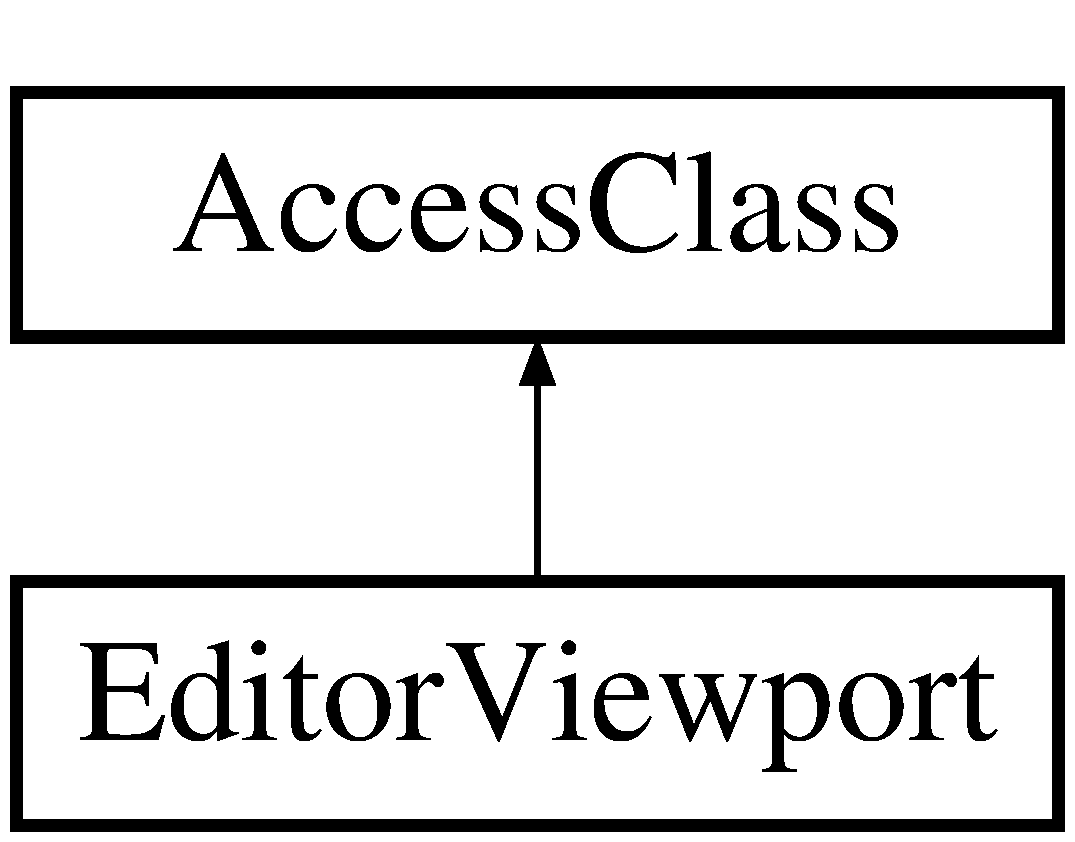
\includegraphics[height=2.000000cm]{classEditorViewport}
\end{center}
\end{figure}
\subsection*{Public Member Functions}
\begin{DoxyCompactItemize}
\item 
\hypertarget{classEditorViewport_a9e1acddb0e1bd9de0ee5c144d65d231b}{void {\bfseries paint} (Graphics \&g)}\label{classEditorViewport_a9e1acddb0e1bd9de0ee5c144d65d231b}

\item 
\hypertarget{classEditorViewport_ad0b9dfd4b77ca870e76f174032e12fd0}{void {\bfseries delete\-Node} (\hyperlink{classGenericEditor}{Generic\-Editor} $\ast$editor)}\label{classEditorViewport_ad0b9dfd4b77ca870e76f174032e12fd0}

\item 
\hypertarget{classEditorViewport_aa788025ac31951eb6b3db55f5da19350}{void {\bfseries select\-Editor} (\hyperlink{classGenericEditor}{Generic\-Editor} $\ast$e)}\label{classEditorViewport_aa788025ac31951eb6b3db55f5da19350}

\item 
\hypertarget{classEditorViewport_a48ffa818358a263ac61221d5e94a14cc}{void {\bfseries make\-Editor\-Visible} (\hyperlink{classGenericEditor}{Generic\-Editor} $\ast$e, bool highlight=true)}\label{classEditorViewport_a48ffa818358a263ac61221d5e94a14cc}

\item 
\hypertarget{classEditorViewport_a70a4e6431ea881b26efcecab2ce9f736}{void {\bfseries make\-Editor\-Visible\-And\-Update\-Settings} (\hyperlink{classGenericEditor}{Generic\-Editor} $\ast$e)}\label{classEditorViewport_a70a4e6431ea881b26efcecab2ce9f736}

\item 
\hypertarget{classEditorViewport_a2537b32aa2b8e90835770e5543ba3da7}{void {\bfseries refresh\-Editors} ()}\label{classEditorViewport_a2537b32aa2b8e90835770e5543ba3da7}

\item 
\hypertarget{classEditorViewport_a02c672bb7b4695eec9c6c61eaac389bf}{void {\bfseries clear\-Signal\-Chain} ()}\label{classEditorViewport_a02c672bb7b4695eec9c6c61eaac389bf}

\item 
\hypertarget{classEditorViewport_a507e141c15a124aef3c307bab7e4e5c6}{void {\bfseries signal\-Chain\-Can\-Be\-Edited} (bool t)}\label{classEditorViewport_a507e141c15a124aef3c307bab7e4e5c6}

\item 
\hypertarget{classEditorViewport_adb0fd596073954d1ece43739e5925d33}{bool {\bfseries is\-Interested\-In\-Drag\-Source} (const String \&, Component $\ast$)}\label{classEditorViewport_adb0fd596073954d1ece43739e5925d33}

\item 
\hypertarget{classEditorViewport_a14cb153a6f1ca97584c3bfa88d5839e4}{void {\bfseries item\-Drag\-Enter} (const String \&, Component $\ast$, int, int)}\label{classEditorViewport_a14cb153a6f1ca97584c3bfa88d5839e4}

\item 
\hypertarget{classEditorViewport_a99630d7cff4060355eb33b523a1ff662}{void {\bfseries item\-Drag\-Move} (const String \&, Component $\ast$, int, int)}\label{classEditorViewport_a99630d7cff4060355eb33b523a1ff662}

\item 
\hypertarget{classEditorViewport_aa0a6e241e6900665b4cd83ca75da169c}{void {\bfseries item\-Drag\-Exit} (const String \&, Component $\ast$)}\label{classEditorViewport_aa0a6e241e6900665b4cd83ca75da169c}

\item 
\hypertarget{classEditorViewport_a28feb4315615bf02650df7d9df8230da}{void {\bfseries item\-Dropped} (const String \&source\-Description, Component $\ast$, int, int)}\label{classEditorViewport_a28feb4315615bf02650df7d9df8230da}

\item 
\hypertarget{classEditorViewport_ae5ea71d59fb37b2888a451d7ad96a0af}{void {\bfseries mouse\-Down} (const Mouse\-Event \&e)}\label{classEditorViewport_ae5ea71d59fb37b2888a451d7ad96a0af}

\item 
\hypertarget{classEditorViewport_a0945e16ac793100d8a30d1f0b9dd7618}{void {\bfseries mouse\-Drag} (const Mouse\-Event \&e)}\label{classEditorViewport_a0945e16ac793100d8a30d1f0b9dd7618}

\item 
\hypertarget{classEditorViewport_a839c651c6aaf978166a59eb8268c9728}{void {\bfseries mouse\-Up} (const Mouse\-Event \&e)}\label{classEditorViewport_a839c651c6aaf978166a59eb8268c9728}

\item 
\hypertarget{classEditorViewport_a30efef0c60d508fdb5f94efc6729e315}{void {\bfseries mouse\-Exit} (const Mouse\-Event \&e)}\label{classEditorViewport_a30efef0c60d508fdb5f94efc6729e315}

\item 
\hypertarget{classEditorViewport_a949986b1e5866860a76b91f96fc68c54}{bool {\bfseries key\-Pressed} (const Key\-Press \&key)}\label{classEditorViewport_a949986b1e5866860a76b91f96fc68c54}

\item 
\hypertarget{classEditorViewport_a49167a0ba2902fc95199ca4897f773c6}{void {\bfseries move\-Selection} (const Key\-Press \&key)}\label{classEditorViewport_a49167a0ba2902fc95199ca4897f773c6}

\item 
\hypertarget{classEditorViewport_a993f75f13ab62e1cea1ce38da1f046d5}{void {\bfseries button\-Clicked} (Button $\ast$button)}\label{classEditorViewport_a993f75f13ab62e1cea1ce38da1f046d5}

\item 
\hypertarget{classEditorViewport_aea2c840f1ca1309f483b7ff600e9e4ad}{Array$<$ \hyperlink{classSignalChainTabButton}{Signal\-Chain\-Tab\-Button} \\*
$\ast$, Critical\-Section $>$ {\bfseries request\-Signal\-Chain} ()}\label{classEditorViewport_aea2c840f1ca1309f483b7ff600e9e4ad}

\item 
\hypertarget{classEditorViewport_a00ade83a870133a9ddf339a38dd06b3c}{const String {\bfseries save\-State} ()}\label{classEditorViewport_a00ade83a870133a9ddf339a38dd06b3c}

\item 
\hypertarget{classEditorViewport_a2ae2ff8e05fca5d7717fbce441fb2412}{const String {\bfseries load\-State} ()}\label{classEditorViewport_a2ae2ff8e05fca5d7717fbce441fb2412}

\item 
\hypertarget{classEditorViewport_a231c3600cecadafa2b6c01dc39515c7b}{Xml\-Element $\ast$ {\bfseries create\-Node\-Xml} (\hyperlink{classGenericEditor}{Generic\-Editor} $\ast$, int)}\label{classEditorViewport_a231c3600cecadafa2b6c01dc39515c7b}

\item 
\hypertarget{classEditorViewport_a6d055783c0fe0c8cea45a9924b45d99a}{Xml\-Element $\ast$ {\bfseries switch\-Node\-Xml} (\hyperlink{classGenericProcessor}{Generic\-Processor} $\ast$)}\label{classEditorViewport_a6d055783c0fe0c8cea45a9924b45d99a}

\item 
\hypertarget{classEditorViewport_aada77ca562341a093410527034b10818}{void {\bfseries check\-Scroll\-Buttons} (int top\-Tab)}\label{classEditorViewport_aada77ca562341a093410527034b10818}

\item 
\hypertarget{classEditorViewport_a1b5cea1e2a181d39375b025a5c1dd047}{bool {\bfseries is\-Signal\-Chain\-Empty} ()}\label{classEditorViewport_a1b5cea1e2a181d39375b025a5c1dd047}

\end{DoxyCompactItemize}
\subsection*{Public Attributes}
\begin{DoxyCompactItemize}
\item 
\hypertarget{classEditorViewport_ab05cd676ab48b8e252d56d1fb9f07d4f}{int {\bfseries leftmost\-Editor}}\label{classEditorViewport_ab05cd676ab48b8e252d56d1fb9f07d4f}

\item 
\hypertarget{classEditorViewport_a09ffd88dead53e37ce7701adeda3ce8a}{File {\bfseries current\-File}}\label{classEditorViewport_a09ffd88dead53e37ce7701adeda3ce8a}

\end{DoxyCompactItemize}
\subsection*{Private Types}
\begin{DoxyCompactItemize}
\item 
enum {\bfseries actions} \{ \\*
{\bfseries A\-D\-D}, 
{\bfseries M\-O\-V\-E}, 
{\bfseries R\-E\-M\-O\-V\-E}, 
{\bfseries A\-C\-T\-I\-V\-A\-T\-E}, 
\\*
{\bfseries U\-P\-D\-A\-T\-E}
 \}
\item 
enum {\bfseries directions1} \{ {\bfseries L\-E\-F\-T}, 
{\bfseries R\-I\-G\-H\-T}
 \}
\item 
enum {\bfseries directions2} \{ {\bfseries U\-P}, 
{\bfseries D\-O\-W\-N}
 \}
\end{DoxyCompactItemize}
\subsection*{Private Member Functions}
\begin{DoxyCompactItemize}
\item 
\hypertarget{classEditorViewport_a93de817036f82c0a1253f81343e34347}{void {\bfseries create\-New\-Tab} (\hyperlink{classGenericEditor}{Generic\-Editor} $\ast$editor)}\label{classEditorViewport_a93de817036f82c0a1253f81343e34347}

\item 
\hypertarget{classEditorViewport_ad78263f172f5ee69109bcdb728e22aeb}{void {\bfseries remove\-Tab} (int tab\-Index)}\label{classEditorViewport_ad78263f172f5ee69109bcdb728e22aeb}

\item 
\hypertarget{classEditorViewport_a1c0ecac694cc8340d464391778b5f727}{void {\bfseries resized} ()}\label{classEditorViewport_a1c0ecac694cc8340d464391778b5f727}

\item 
\hypertarget{classEditorViewport_a3216cc1566e1b5e891b1825436abb9dc}{{\bfseries J\-U\-C\-E\-\_\-\-D\-E\-C\-L\-A\-R\-E\-\_\-\-N\-O\-N\-\_\-\-C\-O\-P\-Y\-A\-B\-L\-E\-\_\-\-W\-I\-T\-H\-\_\-\-L\-E\-A\-K\-\_\-\-D\-E\-T\-E\-C\-T\-O\-R} (\hyperlink{classEditorViewport}{Editor\-Viewport})}\label{classEditorViewport_a3216cc1566e1b5e891b1825436abb9dc}

\end{DoxyCompactItemize}
\subsection*{Private Attributes}
\begin{DoxyCompactItemize}
\item 
\hypertarget{classEditorViewport_aebcce72fe2d98eed5690cdea87bbd776}{String {\bfseries message}}\label{classEditorViewport_aebcce72fe2d98eed5690cdea87bbd776}

\item 
\hypertarget{classEditorViewport_a152689484821c227a7909c6087b41e6c}{bool {\bfseries something\-Is\-Being\-Dragged\-Over}}\label{classEditorViewport_a152689484821c227a7909c6087b41e6c}

\item 
\hypertarget{classEditorViewport_a04fad22528a1dd4d5d68fd6cec4d0dd4}{bool {\bfseries shift\-Down}}\label{classEditorViewport_a04fad22528a1dd4d5d68fd6cec4d0dd4}

\item 
\hypertarget{classEditorViewport_ada0e62d14a51a7ffda1e396a5b66061c}{bool {\bfseries can\-Edit}}\label{classEditorViewport_ada0e62d14a51a7ffda1e396a5b66061c}

\item 
\hypertarget{classEditorViewport_aa4e7f71ad4823d393a489853d2760ba8}{\hyperlink{classGenericEditor}{Generic\-Editor} $\ast$ {\bfseries last\-Editor}}\label{classEditorViewport_aa4e7f71ad4823d393a489853d2760ba8}

\item 
\hypertarget{classEditorViewport_a7964a4d304213a3d5a40c3f7ea48257e}{\hyperlink{classGenericEditor}{Generic\-Editor} $\ast$ {\bfseries last\-Editor\-Clicked}}\label{classEditorViewport_a7964a4d304213a3d5a40c3f7ea48257e}

\item 
\hypertarget{classEditorViewport_a4b8c16b1db82e6f7949be357ee9ce644}{int {\bfseries selection\-Index}}\label{classEditorViewport_a4b8c16b1db82e6f7949be357ee9ce644}

\item 
\hypertarget{classEditorViewport_afb84ce94749157028397417b95b70aba}{Array$<$ \hyperlink{classGenericEditor}{Generic\-Editor} \\*
$\ast$, Critical\-Section $>$ {\bfseries editor\-Array}}\label{classEditorViewport_afb84ce94749157028397417b95b70aba}

\item 
\hypertarget{classEditorViewport_a1f7e1003e9ad42e10eb6154a756735ec}{Array$<$ \hyperlink{classSignalChainTabButton}{Signal\-Chain\-Tab\-Button} \\*
$\ast$, Critical\-Section $>$ {\bfseries signal\-Chain\-Array}}\label{classEditorViewport_a1f7e1003e9ad42e10eb6154a756735ec}

\item 
\hypertarget{classEditorViewport_addbe939901e75ce05fd7c6bc25ed8099}{Scoped\-Pointer$<$ \hyperlink{classSignalChainManager}{Signal\-Chain\-Manager} $>$ {\bfseries signal\-Chain\-Manager}}\label{classEditorViewport_addbe939901e75ce05fd7c6bc25ed8099}

\item 
\hypertarget{classEditorViewport_a742248bc2ce37fd7e511e027b8369579}{Font {\bfseries font}}\label{classEditorViewport_a742248bc2ce37fd7e511e027b8369579}

\item 
\hypertarget{classEditorViewport_a0a000a563a6839777c1e37a382b99990}{Image {\bfseries source\-Drop\-Image}}\label{classEditorViewport_a0a000a563a6839777c1e37a382b99990}

\item 
\hypertarget{classEditorViewport_a6efd91ca1ea24c0f728c420f5a9a5c3d}{int {\bfseries border\-Size}}\label{classEditorViewport_a6efd91ca1ea24c0f728c420f5a9a5c3d}

\item 
\hypertarget{classEditorViewport_a9a6174e30d66ec370e34380346d31880}{int {\bfseries tab\-Size}}\label{classEditorViewport_a9a6174e30d66ec370e34380346d31880}

\item 
\hypertarget{classEditorViewport_aea33d0cdc5fdd65ad1ba286ce8b160c8}{int {\bfseries tab\-Button\-Size}}\label{classEditorViewport_aea33d0cdc5fdd65ad1ba286ce8b160c8}

\item 
\hypertarget{classEditorViewport_a4232494d0a71542296b93c7eaa7da579}{int {\bfseries insertion\-Point}}\label{classEditorViewport_a4232494d0a71542296b93c7eaa7da579}

\item 
\hypertarget{classEditorViewport_a26f22e7827e51fb66d3a5262e90ef6ab}{bool {\bfseries component\-Wants\-To\-Move}}\label{classEditorViewport_a26f22e7827e51fb66d3a5262e90ef6ab}

\item 
\hypertarget{classEditorViewport_a05ba5e48e39f716d312c1667e9a80954}{int {\bfseries index\-Of\-Moving\-Component}}\label{classEditorViewport_a05ba5e48e39f716d312c1667e9a80954}

\item 
\hypertarget{classEditorViewport_ad10d97f0189b0c4bba4d3998f91c24e2}{int {\bfseries current\-Tab}}\label{classEditorViewport_ad10d97f0189b0c4bba4d3998f91c24e2}

\item 
\hypertarget{classEditorViewport_acac49fef76c61a2c390f61940d859283}{\hyperlink{classEditorScrollButton}{Editor\-Scroll\-Button} $\ast$ {\bfseries left\-Button}}\label{classEditorViewport_acac49fef76c61a2c390f61940d859283}

\item 
\hypertarget{classEditorViewport_a0683397c25ec6c4193322cb44b317d10}{\hyperlink{classEditorScrollButton}{Editor\-Scroll\-Button} $\ast$ {\bfseries right\-Button}}\label{classEditorViewport_a0683397c25ec6c4193322cb44b317d10}

\item 
\hypertarget{classEditorViewport_aca0a1943bce0ec9b5950b6c395df2094}{\hyperlink{classSignalChainScrollButton}{Signal\-Chain\-Scroll\-Button} $\ast$ {\bfseries up\-Button}}\label{classEditorViewport_aca0a1943bce0ec9b5950b6c395df2094}

\item 
\hypertarget{classEditorViewport_a0749ed016653202a8bed9447b45de1b6}{\hyperlink{classSignalChainScrollButton}{Signal\-Chain\-Scroll\-Button} $\ast$ {\bfseries down\-Button}}\label{classEditorViewport_a0749ed016653202a8bed9447b45de1b6}

\end{DoxyCompactItemize}


The documentation for this class was generated from the following file\-:\begin{DoxyCompactItemize}
\item 
U\-I/Editor\-Viewport.\-h\end{DoxyCompactItemize}

\hypertarget{classEditorViewportButton}{\section{Editor\-Viewport\-Button Class Reference}
\label{classEditorViewportButton}\index{Editor\-Viewport\-Button@{Editor\-Viewport\-Button}}
}
\subsection*{Public Member Functions}
\begin{DoxyCompactItemize}
\item 
\hypertarget{classEditorViewportButton_a4aacb445c8515a6d5713b3542d12d4d5}{{\bfseries Editor\-Viewport\-Button} (\hyperlink{classUIComponent}{U\-I\-Component} $\ast$ui)}\label{classEditorViewportButton_a4aacb445c8515a6d5713b3542d12d4d5}

\item 
\hypertarget{classEditorViewportButton_ac6ede44d50ca1bb6879c4dbe469520c0}{bool {\bfseries is\-Open} ()}\label{classEditorViewportButton_ac6ede44d50ca1bb6879c4dbe469520c0}

\item 
\hypertarget{classEditorViewportButton_aa33c3aaa4badc7f52dad8ed2e4812eee}{void {\bfseries new\-Open\-G\-L\-Context\-Created} ()}\label{classEditorViewportButton_aa33c3aaa4badc7f52dad8ed2e4812eee}

\item 
\hypertarget{classEditorViewportButton_aa80cea482fd8a27fe27ce42334772b4c}{void {\bfseries render\-Open\-G\-L} ()}\label{classEditorViewportButton_aa80cea482fd8a27fe27ce42334772b4c}

\item 
\hypertarget{classEditorViewportButton_ac59d52952099fd8e225ad2d08eaff16c}{void {\bfseries draw\-Name} ()}\label{classEditorViewportButton_ac59d52952099fd8e225ad2d08eaff16c}

\item 
\hypertarget{classEditorViewportButton_ae802cc7116cb80264fb137aa67468402}{void {\bfseries draw\-Button} ()}\label{classEditorViewportButton_ae802cc7116cb80264fb137aa67468402}

\item 
\hypertarget{classEditorViewportButton_a857d674515278d616cec9b26bb44330d}{void {\bfseries toggle\-State} ()}\label{classEditorViewportButton_a857d674515278d616cec9b26bb44330d}

\item 
\hypertarget{classEditorViewportButton_adc62cdc302d3fe04080459aa0ec97e73}{void {\bfseries mouse\-Down} (const Mouse\-Event \&e)}\label{classEditorViewportButton_adc62cdc302d3fe04080459aa0ec97e73}

\end{DoxyCompactItemize}
\subsection*{Private Attributes}
\begin{DoxyCompactItemize}
\item 
\hypertarget{classEditorViewportButton_a76782e6db44130c925ca51412ea82b2b}{\hyperlink{classUIComponent}{U\-I\-Component} $\ast$ {\bfseries U\-I}}\label{classEditorViewportButton_a76782e6db44130c925ca51412ea82b2b}

\item 
\hypertarget{classEditorViewportButton_a66ba90699ffe12aa26640fb21a9ab2e0}{bool {\bfseries open}}\label{classEditorViewportButton_a66ba90699ffe12aa26640fb21a9ab2e0}

\item 
\hypertarget{classEditorViewportButton_ac95459c5ba70fe32af94e07c40299548}{F\-T\-Pixmap\-Font $\ast$ {\bfseries font}}\label{classEditorViewportButton_ac95459c5ba70fe32af94e07c40299548}

\end{DoxyCompactItemize}


The documentation for this class was generated from the following file\-:\begin{DoxyCompactItemize}
\item 
U\-I/U\-I\-Component.\-h\end{DoxyCompactItemize}

\hypertarget{structSpikeDetector_1_1Electrode}{\section{Spike\-Detector\-:\-:Electrode Struct Reference}
\label{structSpikeDetector_1_1Electrode}\index{Spike\-Detector\-::\-Electrode@{Spike\-Detector\-::\-Electrode}}
}
\subsection*{Public Attributes}
\begin{DoxyCompactItemize}
\item 
\hypertarget{structSpikeDetector_1_1Electrode_a27773e746444f91b64a02e262f0f693e}{String {\bfseries name}}\label{structSpikeDetector_1_1Electrode_a27773e746444f91b64a02e262f0f693e}

\item 
\hypertarget{structSpikeDetector_1_1Electrode_af4d01374066d650c8e33009e659cfabd}{int {\bfseries num\-Channels}}\label{structSpikeDetector_1_1Electrode_af4d01374066d650c8e33009e659cfabd}

\item 
\hypertarget{structSpikeDetector_1_1Electrode_a29c1a3dffd5218caf29bce86c3b2ae12}{int {\bfseries pre\-Peak\-Samples}}\label{structSpikeDetector_1_1Electrode_a29c1a3dffd5218caf29bce86c3b2ae12}

\item 
\hypertarget{structSpikeDetector_1_1Electrode_a1b94c165f436b181dbaae51429312e8f}{int {\bfseries post\-Peak\-Samples}}\label{structSpikeDetector_1_1Electrode_a1b94c165f436b181dbaae51429312e8f}

\item 
\hypertarget{structSpikeDetector_1_1Electrode_a80465ab3daafd065759f97b7016bd819}{int {\bfseries last\-Buffer\-Index}}\label{structSpikeDetector_1_1Electrode_a80465ab3daafd065759f97b7016bd819}

\item 
\hypertarget{structSpikeDetector_1_1Electrode_a0110e135ec9b668c7e4bc36f17f0fd96}{int $\ast$ {\bfseries channels}}\label{structSpikeDetector_1_1Electrode_a0110e135ec9b668c7e4bc36f17f0fd96}

\item 
\hypertarget{structSpikeDetector_1_1Electrode_a69ebc7bf7878c7050d58e397da658dec}{double $\ast$ {\bfseries thresholds}}\label{structSpikeDetector_1_1Electrode_a69ebc7bf7878c7050d58e397da658dec}

\item 
\hypertarget{structSpikeDetector_1_1Electrode_a571092ec10ce636abc11ef782d4f329f}{bool $\ast$ {\bfseries is\-Active}}\label{structSpikeDetector_1_1Electrode_a571092ec10ce636abc11ef782d4f329f}

\end{DoxyCompactItemize}


The documentation for this struct was generated from the following file\-:\begin{DoxyCompactItemize}
\item 
Processors/Spike\-Detector.\-h\end{DoxyCompactItemize}

\hypertarget{classElectrodeButton}{\section{Electrode\-Button Class Reference}
\label{classElectrodeButton}\index{Electrode\-Button@{Electrode\-Button}}
}
\subsection*{Public Member Functions}
\begin{DoxyCompactItemize}
\item 
\hypertarget{classElectrodeButton_a15999b20ddc88248d2de0bf2e78c5a26}{{\bfseries Electrode\-Button} (int chan\-\_\-)}\label{classElectrodeButton_a15999b20ddc88248d2de0bf2e78c5a26}

\item 
\hypertarget{classElectrodeButton_a1738d6809dd3fe22638a25b23df4e9b1}{int {\bfseries get\-Channel\-Num} ()}\label{classElectrodeButton_a1738d6809dd3fe22638a25b23df4e9b1}

\item 
\hypertarget{classElectrodeButton_af82d6cf490fdce1d729d53d1ec722f13}{void {\bfseries set\-Channel\-Num} (int i)}\label{classElectrodeButton_af82d6cf490fdce1d729d53d1ec722f13}

\end{DoxyCompactItemize}
\subsection*{Private Member Functions}
\begin{DoxyCompactItemize}
\item 
\hypertarget{classElectrodeButton_a4f6f76c9773cf7ef40cdbb8fbb82e938}{void {\bfseries paint\-Button} (Graphics \&g, bool is\-Mouse\-Over, bool is\-Button\-Down)}\label{classElectrodeButton_a4f6f76c9773cf7ef40cdbb8fbb82e938}

\end{DoxyCompactItemize}
\subsection*{Private Attributes}
\begin{DoxyCompactItemize}
\item 
\hypertarget{classElectrodeButton_a0be15afb8675a5cad16d2b1bd13f5648}{int {\bfseries chan}}\label{classElectrodeButton_a0be15afb8675a5cad16d2b1bd13f5648}

\end{DoxyCompactItemize}


The documentation for this class was generated from the following file\-:\begin{DoxyCompactItemize}
\item 
Processors/\-Editors/Spike\-Detector\-Editor.\-h\end{DoxyCompactItemize}

\hypertarget{classElectrodeEditorButton}{\section{Electrode\-Editor\-Button Class Reference}
\label{classElectrodeEditorButton}\index{Electrode\-Editor\-Button@{Electrode\-Editor\-Button}}
}
\subsection*{Public Member Functions}
\begin{DoxyCompactItemize}
\item 
\hypertarget{classElectrodeEditorButton_a41ee69863e123b19d0cb5407532edf39}{{\bfseries Electrode\-Editor\-Button} (const String \&name\-\_\-, Font font\-\_\-)}\label{classElectrodeEditorButton_a41ee69863e123b19d0cb5407532edf39}

\end{DoxyCompactItemize}
\subsection*{Private Member Functions}
\begin{DoxyCompactItemize}
\item 
\hypertarget{classElectrodeEditorButton_ac93bd656e8c2fa725ad1406bccdd8e30}{void {\bfseries paint\-Button} (Graphics \&g, bool is\-Mouse\-Over, bool is\-Button\-Down)}\label{classElectrodeEditorButton_ac93bd656e8c2fa725ad1406bccdd8e30}

\end{DoxyCompactItemize}
\subsection*{Private Attributes}
\begin{DoxyCompactItemize}
\item 
\hypertarget{classElectrodeEditorButton_a0722a63b6adf39abe15524e76df92f5e}{const String {\bfseries name}}\label{classElectrodeEditorButton_a0722a63b6adf39abe15524e76df92f5e}

\item 
\hypertarget{classElectrodeEditorButton_a8efaf1a6be14e7fe174e30fca8d50a7f}{Font {\bfseries font}}\label{classElectrodeEditorButton_a8efaf1a6be14e7fe174e30fca8d50a7f}

\end{DoxyCompactItemize}


The documentation for this class was generated from the following file\-:\begin{DoxyCompactItemize}
\item 
Processors/\-Editors/Spike\-Detector\-Editor.\-h\end{DoxyCompactItemize}

\hypertarget{classElectrodePlot}{\section{Electrode\-Plot Class Reference}
\label{classElectrodePlot}\index{Electrode\-Plot@{Electrode\-Plot}}
}
Inheritance diagram for Electrode\-Plot\-:\begin{figure}[H]
\begin{center}
\leavevmode
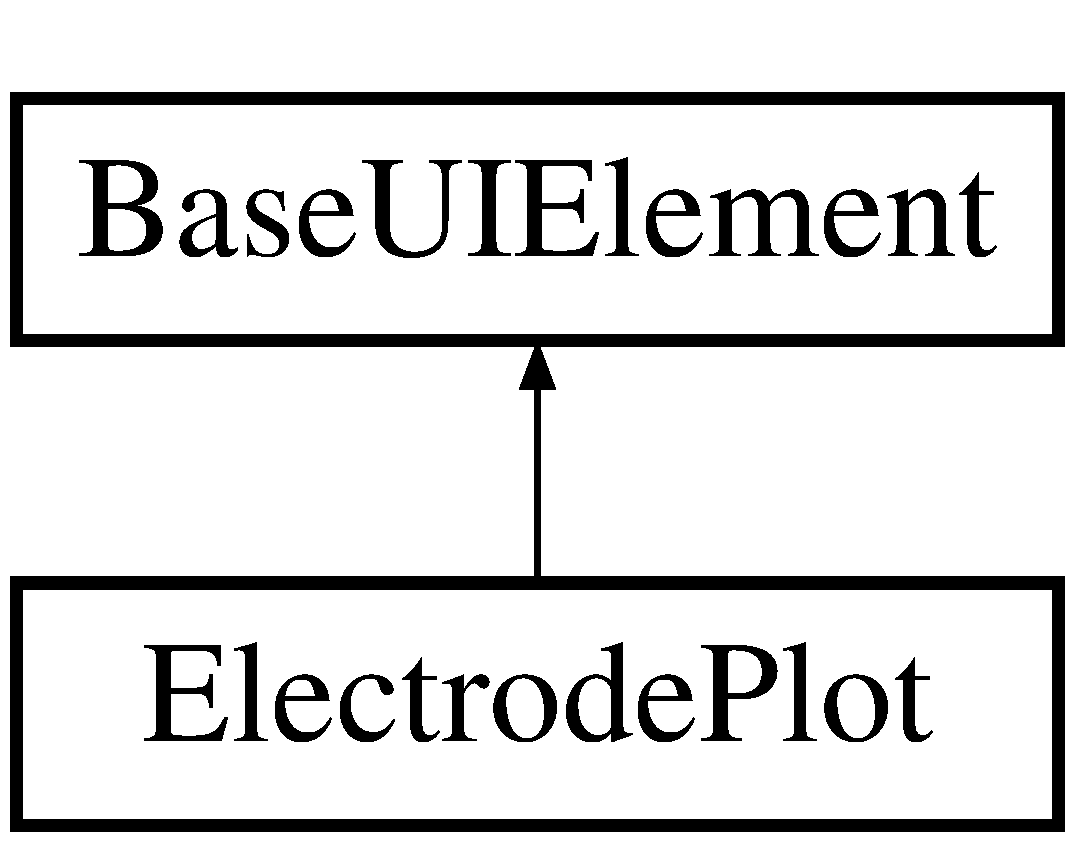
\includegraphics[height=2.000000cm]{classElectrodePlot}
\end{center}
\end{figure}
\subsection*{Public Member Functions}
\begin{DoxyCompactItemize}
\item 
\hypertarget{classElectrodePlot_a38ca347b89d0a8388e3b8874a9c8291d}{{\bfseries Electrode\-Plot} (int x, int y, int w, int h)}\label{classElectrodePlot_a38ca347b89d0a8388e3b8874a9c8291d}

\item 
\hypertarget{classElectrodePlot_ab222ba4b5332926e5548770a90b72c37}{void {\bfseries init\-Axes} ()}\label{classElectrodePlot_ab222ba4b5332926e5548770a90b72c37}

\item 
\hypertarget{classElectrodePlot_a6a135cde6e380524e7ee2eecfaa7b241}{void {\bfseries redraw} ()}\label{classElectrodePlot_a6a135cde6e380524e7ee2eecfaa7b241}

\item 
\hypertarget{classElectrodePlot_a4cbd5761bd66e3a278f7e0d0e917fb27}{void {\bfseries set\-Enabled} (bool enabled)}\label{classElectrodePlot_a4cbd5761bd66e3a278f7e0d0e917fb27}

\item 
\hypertarget{classElectrodePlot_a167ae69b1e5f45b57371aea91f53fa1b}{bool {\bfseries get\-Enabled} ()}\label{classElectrodePlot_a167ae69b1e5f45b57371aea91f53fa1b}

\item 
\hypertarget{classElectrodePlot_a619fae24731c9abd554067f22bd47641}{void {\bfseries set\-Position} (int, int, double, double)}\label{classElectrodePlot_a619fae24731c9abd554067f22bd47641}

\item 
\hypertarget{classElectrodePlot_a3cd86a9218c81d2217624851fed1c930}{void {\bfseries get\-Preferred\-Dimensions} (double $\ast$, double $\ast$)}\label{classElectrodePlot_a3cd86a9218c81d2217624851fed1c930}

\item 
\hypertarget{classElectrodePlot_a8d70b0e45c5915593deb19485d5ab541}{int {\bfseries get\-Number\-Of\-Axes} ()}\label{classElectrodePlot_a8d70b0e45c5915593deb19485d5ab541}

\item 
\hypertarget{classElectrodePlot_a560bceaa1b9d763bc36756ce5a00da82}{void {\bfseries mouse\-Down} (int x, int y)}\label{classElectrodePlot_a560bceaa1b9d763bc36756ce5a00da82}

\item 
\hypertarget{classElectrodePlot_ac44b6d1e18c9a6d8f9d6ae4df1c626b4}{void {\bfseries mouse\-Drag\-X} (int dx, bool shift, bool ctr)}\label{classElectrodePlot_ac44b6d1e18c9a6d8f9d6ae4df1c626b4}

\item 
\hypertarget{classElectrodePlot_a5d165e2e1907d1d8092b124943ab6708}{void {\bfseries mouse\-Drag\-Y} (int dy, bool shift, bool ctr)}\label{classElectrodePlot_a5d165e2e1907d1d8092b124943ab6708}

\item 
\hypertarget{classElectrodePlot_a6bf5d37448860059c5e2b8366d08a112}{bool {\bfseries process\-Key\-Event} (\hyperlink{structSimpleKeyEvent}{Simple\-Key\-Event} k)}\label{classElectrodePlot_a6bf5d37448860059c5e2b8366d08a112}

\item 
\hypertarget{classElectrodePlot_ae2aa2a0ccd12d7df8fdf9d563e239298}{void {\bfseries process\-Spike\-Object} (\hyperlink{structSpikeObject}{Spike\-Object} s)}\label{classElectrodePlot_ae2aa2a0ccd12d7df8fdf9d563e239298}

\end{DoxyCompactItemize}
\subsection*{Private Member Functions}
\begin{DoxyCompactItemize}
\item 
\hypertarget{classElectrodePlot_a2fa9ec77bee7b1820b336fc7edae240a}{void {\bfseries init\-Limits} ()}\label{classElectrodePlot_a2fa9ec77bee7b1820b336fc7edae240a}

\end{DoxyCompactItemize}
\subsection*{Private Attributes}
\begin{DoxyCompactItemize}
\item 
\hypertarget{classElectrodePlot_a237f3969769bc74af0006c7a79d07e91}{bool {\bfseries enabled}}\label{classElectrodePlot_a237f3969769bc74af0006c7a79d07e91}

\item 
\hypertarget{classElectrodePlot_ae0a7e535cdff2c9a50e2eb2eb0cf9218}{bool {\bfseries limits\-Changed}}\label{classElectrodePlot_ae0a7e535cdff2c9a50e2eb2eb0cf9218}

\item 
\hypertarget{classElectrodePlot_a825cf17531fb7811bea0e55ff9a81cab}{double {\bfseries limits} \mbox{[}1\mbox{]}\mbox{[}2\mbox{]}}\label{classElectrodePlot_a825cf17531fb7811bea0e55ff9a81cab}

\item 
\hypertarget{classElectrodePlot_a2b5edc11ad304fbf2702377462b0ca28}{\hyperlink{classWaveAxes}{Wave\-Axes} {\bfseries axes}}\label{classElectrodePlot_a2b5edc11ad304fbf2702377462b0ca28}

\end{DoxyCompactItemize}
\subsection*{Additional Inherited Members}


The documentation for this class was generated from the following file\-:\begin{DoxyCompactItemize}
\item 
Processors/\-Visualization/\-Spike\-Plotting/Electrode\-Plot.\-h\end{DoxyCompactItemize}

\hypertarget{classEventNode}{\section{Event\-Node Class Reference}
\label{classEventNode}\index{Event\-Node@{Event\-Node}}
}


{\ttfamily \#include $<$Event\-Node.\-h$>$}

Inheritance diagram for Event\-Node\-:\begin{figure}[H]
\begin{center}
\leavevmode
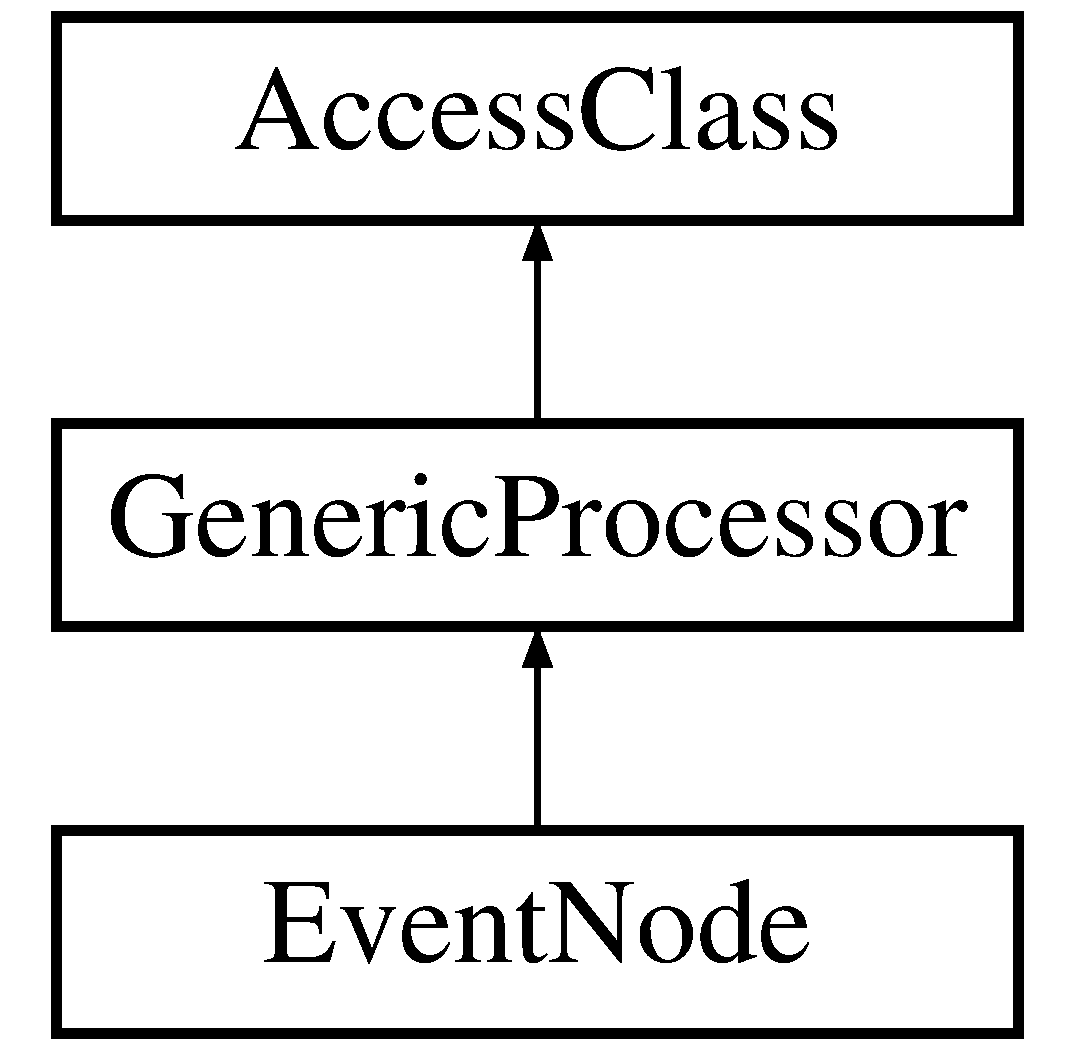
\includegraphics[height=3.000000cm]{classEventNode}
\end{center}
\end{figure}
\subsection*{Public Member Functions}
\begin{DoxyCompactItemize}
\item 
\hypertarget{classEventNode_a28028d513a537386d87dbc925f53261b}{void {\bfseries process} (Audio\-Sample\-Buffer \&buffer, Midi\-Buffer \&midi\-Messages, int \&n\-Samples)}\label{classEventNode_a28028d513a537386d87dbc925f53261b}

\item 
\hypertarget{classEventNode_aae0383ac176ded4cd6788ffb7e8d3aca}{bool {\bfseries is\-Source} ()}\label{classEventNode_aae0383ac176ded4cd6788ffb7e8d3aca}

\item 
\hypertarget{classEventNode_a09c5bc4617e5457bfdfbd4c1811e31f8}{int {\bfseries get\-Default\-Num\-Outputs} ()}\label{classEventNode_a09c5bc4617e5457bfdfbd4c1811e31f8}

\item 
\hypertarget{classEventNode_ad219724f2a2334735574df18a9a47691}{void {\bfseries update\-Settings} ()}\label{classEventNode_ad219724f2a2334735574df18a9a47691}

\item 
\hypertarget{classEventNode_ab66d8a254503f0bbc144ce1072aaf4ac}{Audio\-Processor\-Editor $\ast$ {\bfseries create\-Editor} ()}\label{classEventNode_ab66d8a254503f0bbc144ce1072aaf4ac}

\end{DoxyCompactItemize}
\subsection*{Private Member Functions}
\begin{DoxyCompactItemize}
\item 
\hypertarget{classEventNode_aab376837282cb88b5fd8078ef05e0588}{{\bfseries J\-U\-C\-E\-\_\-\-D\-E\-C\-L\-A\-R\-E\-\_\-\-N\-O\-N\-\_\-\-C\-O\-P\-Y\-A\-B\-L\-E\-\_\-\-W\-I\-T\-H\-\_\-\-L\-E\-A\-K\-\_\-\-D\-E\-T\-E\-C\-T\-O\-R} (\hyperlink{classEventNode}{Event\-Node})}\label{classEventNode_aab376837282cb88b5fd8078ef05e0588}

\end{DoxyCompactItemize}
\subsection*{Private Attributes}
\begin{DoxyCompactItemize}
\item 
\hypertarget{classEventNode_a43dedc33c1fb9d1376c3dff836893194}{float {\bfseries accumulator}}\label{classEventNode_a43dedc33c1fb9d1376c3dff836893194}

\item 
\hypertarget{classEventNode_a992d2481092bf59a56e9544257576abc}{float {\bfseries Hz}}\label{classEventNode_a992d2481092bf59a56e9544257576abc}

\end{DoxyCompactItemize}
\subsection*{Additional Inherited Members}


\subsection{Detailed Description}
Generates events at regular intervals.

\begin{DoxySeeAlso}{See also}
\hyperlink{classGenericProcessor}{Generic\-Processor}, \hyperlink{classEventNodeEditor}{Event\-Node\-Editor} 
\end{DoxySeeAlso}


The documentation for this class was generated from the following file\-:\begin{DoxyCompactItemize}
\item 
Processors/Event\-Node.\-h\end{DoxyCompactItemize}

\hypertarget{classEventNodeEditor}{\section{Event\-Node\-Editor Class Reference}
\label{classEventNodeEditor}\index{Event\-Node\-Editor@{Event\-Node\-Editor}}
}
Inheritance diagram for Event\-Node\-Editor\-:\begin{figure}[H]
\begin{center}
\leavevmode
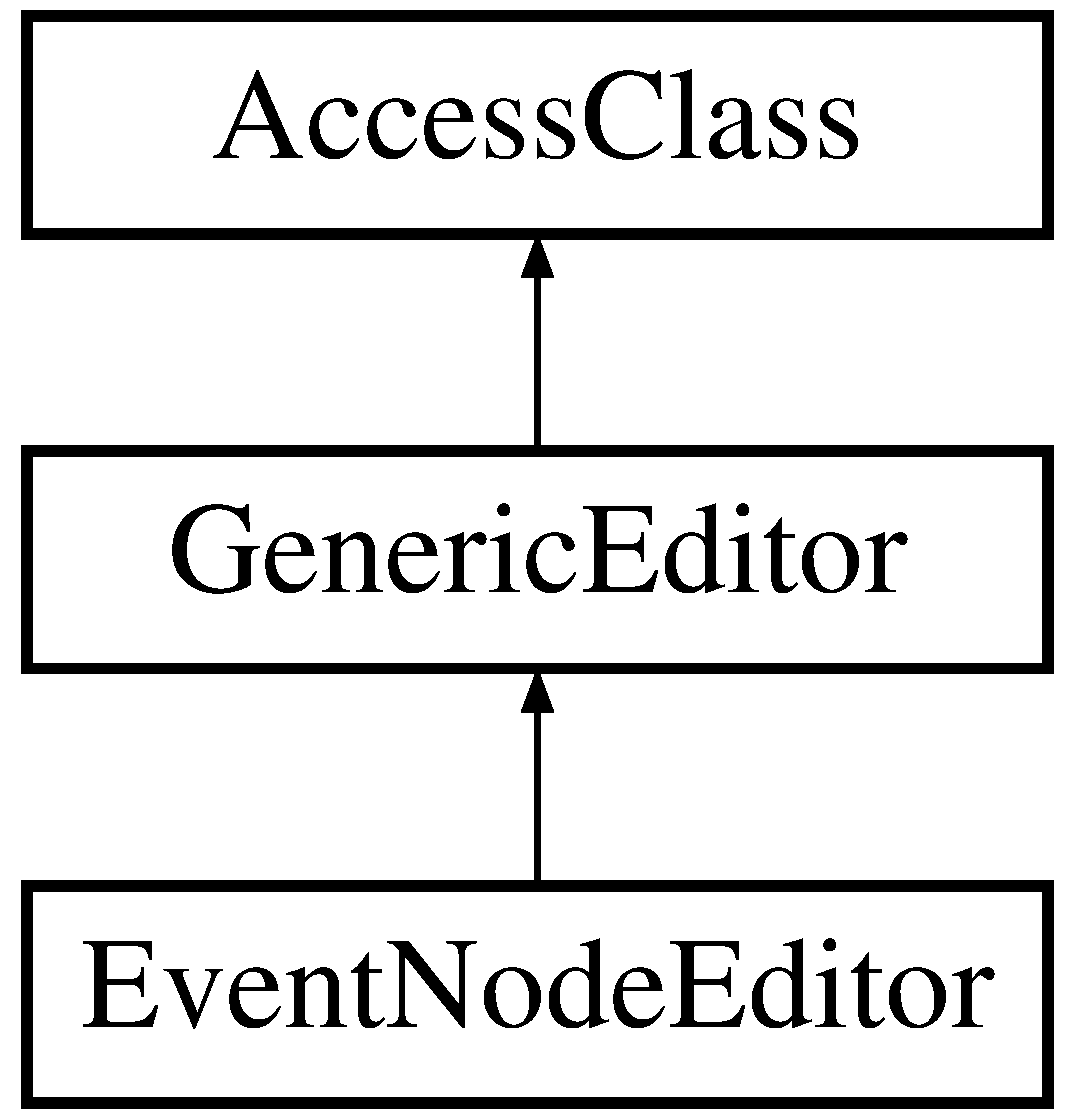
\includegraphics[height=3.000000cm]{classEventNodeEditor}
\end{center}
\end{figure}
\subsection*{Public Member Functions}
\begin{DoxyCompactItemize}
\item 
\hypertarget{classEventNodeEditor_afc10c0210f8f2d53842723ce9d0cb477}{{\bfseries Event\-Node\-Editor} (\hyperlink{classGenericProcessor}{Generic\-Processor} $\ast$parent\-Node)}\label{classEventNodeEditor_afc10c0210f8f2d53842723ce9d0cb477}

\item 
\hypertarget{classEventNodeEditor_a4eef393b8734628eb5b9e4828cf3180e}{void {\bfseries button\-Event} (Button $\ast$button)}\label{classEventNodeEditor_a4eef393b8734628eb5b9e4828cf3180e}

\end{DoxyCompactItemize}
\subsection*{Private Member Functions}
\begin{DoxyCompactItemize}
\item 
\hypertarget{classEventNodeEditor_ae83c947301c0ce834ab1a1acf99c2856}{{\bfseries J\-U\-C\-E\-\_\-\-D\-E\-C\-L\-A\-R\-E\-\_\-\-N\-O\-N\-\_\-\-C\-O\-P\-Y\-A\-B\-L\-E\-\_\-\-W\-I\-T\-H\-\_\-\-L\-E\-A\-K\-\_\-\-D\-E\-T\-E\-C\-T\-O\-R} (\hyperlink{classEventNodeEditor}{Event\-Node\-Editor})}\label{classEventNodeEditor_ae83c947301c0ce834ab1a1acf99c2856}

\end{DoxyCompactItemize}
\subsection*{Additional Inherited Members}


The documentation for this class was generated from the following file\-:\begin{DoxyCompactItemize}
\item 
Processors/\-Editors/Event\-Node\-Editor.\-h\end{DoxyCompactItemize}

\hypertarget{classFileReaderThread}{\section{File\-Reader\-Thread Class Reference}
\label{classFileReaderThread}\index{File\-Reader\-Thread@{File\-Reader\-Thread}}
}
Inheritance diagram for File\-Reader\-Thread\-:\begin{figure}[H]
\begin{center}
\leavevmode
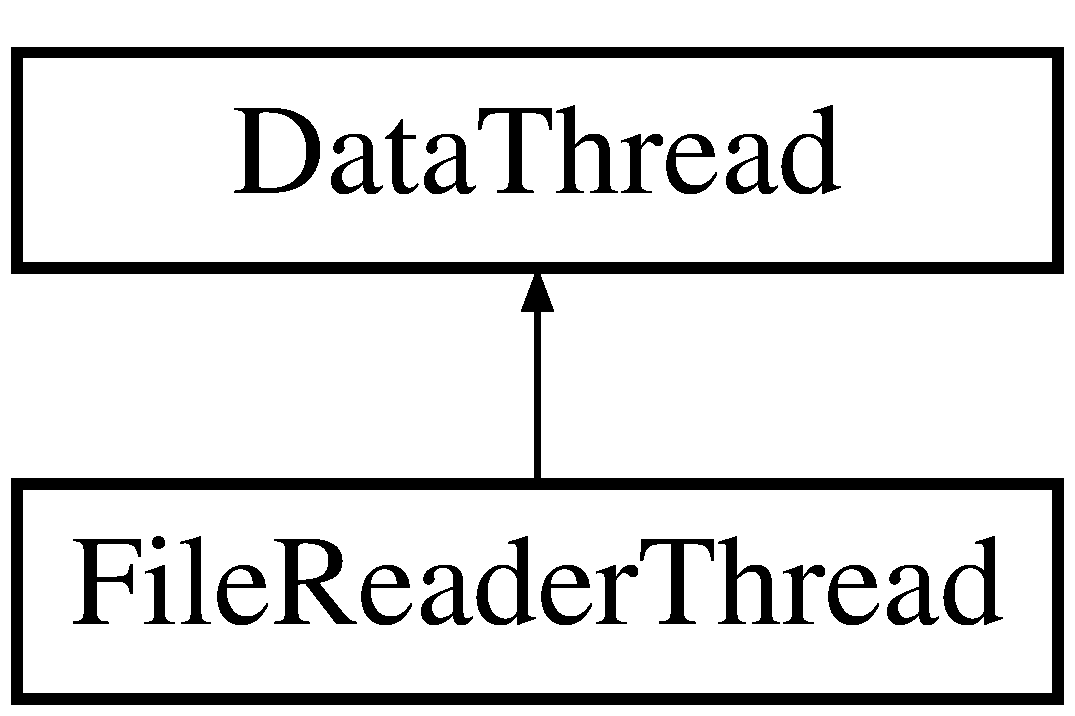
\includegraphics[height=2.000000cm]{classFileReaderThread}
\end{center}
\end{figure}
\subsection*{Public Member Functions}
\begin{DoxyCompactItemize}
\item 
\hypertarget{classFileReaderThread_a9cc610d29b3497c07353551bbec201f2}{{\bfseries File\-Reader\-Thread} (\hyperlink{classSourceNode}{Source\-Node} $\ast$sn)}\label{classFileReaderThread_a9cc610d29b3497c07353551bbec201f2}

\item 
\hypertarget{classFileReaderThread_ae1e58d2033c87cd71cff4d2e45360087}{bool {\bfseries found\-Input\-Source} ()}\label{classFileReaderThread_ae1e58d2033c87cd71cff4d2e45360087}

\item 
\hypertarget{classFileReaderThread_a4d5c3434d7b635d25bbc4c2014b95a61}{bool {\bfseries start\-Acquisition} ()}\label{classFileReaderThread_a4d5c3434d7b635d25bbc4c2014b95a61}

\item 
\hypertarget{classFileReaderThread_ad2abbe666106abe215753a9b3ff328d4}{bool {\bfseries stop\-Acquisition} ()}\label{classFileReaderThread_ad2abbe666106abe215753a9b3ff328d4}

\item 
\hypertarget{classFileReaderThread_aea6f87741b16e78b29f32b2efccf5664}{int {\bfseries get\-Num\-Channels} ()}\label{classFileReaderThread_aea6f87741b16e78b29f32b2efccf5664}

\item 
\hypertarget{classFileReaderThread_ab6360a15dd538bb78dfd3c52fa6fa1d2}{float {\bfseries get\-Sample\-Rate} ()}\label{classFileReaderThread_ab6360a15dd538bb78dfd3c52fa6fa1d2}

\item 
\hypertarget{classFileReaderThread_a50b11fd1f129af9488134d1b6e31e93b}{float {\bfseries get\-Bit\-Volts} ()}\label{classFileReaderThread_a50b11fd1f129af9488134d1b6e31e93b}

\end{DoxyCompactItemize}
\subsection*{Private Member Functions}
\begin{DoxyCompactItemize}
\item 
\hypertarget{classFileReaderThread_a9b29cc5f5357f1f3420ce056e74080e2}{bool {\bfseries update\-Buffer} ()}\label{classFileReaderThread_a9b29cc5f5357f1f3420ce056e74080e2}

\item 
\hypertarget{classFileReaderThread_a315e26b3292c7367955880c796697a77}{{\bfseries J\-U\-C\-E\-\_\-\-D\-E\-C\-L\-A\-R\-E\-\_\-\-N\-O\-N\-\_\-\-C\-O\-P\-Y\-A\-B\-L\-E\-\_\-\-W\-I\-T\-H\-\_\-\-L\-E\-A\-K\-\_\-\-D\-E\-T\-E\-C\-T\-O\-R} (\hyperlink{classFileReaderThread}{File\-Reader\-Thread})}\label{classFileReaderThread_a315e26b3292c7367955880c796697a77}

\end{DoxyCompactItemize}
\subsection*{Private Attributes}
\begin{DoxyCompactItemize}
\item 
\hypertarget{classFileReaderThread_a056a08c6831bcb42f4861af27731bc21}{int {\bfseries samples\-Per\-Block}}\label{classFileReaderThread_a056a08c6831bcb42f4861af27731bc21}

\item 
\hypertarget{classFileReaderThread_ae2eb051836340cf9c11ba910073c53e8}{int {\bfseries length\-Of\-Input\-File}}\label{classFileReaderThread_ae2eb051836340cf9c11ba910073c53e8}

\item 
\hypertarget{classFileReaderThread_a85b607e8d2a3d9031860e8d90a057f73}{int {\bfseries play\-Head}}\label{classFileReaderThread_a85b607e8d2a3d9031860e8d90a057f73}

\item 
\hypertarget{classFileReaderThread_aba27b94f0b117b3e7e15314cb9b6d743}{F\-I\-L\-E $\ast$ {\bfseries input}}\label{classFileReaderThread_aba27b94f0b117b3e7e15314cb9b6d743}

\item 
\hypertarget{classFileReaderThread_ae5b116d0f10ce1d6c44c86f275e42628}{float {\bfseries this\-Sample} \mbox{[}16\mbox{]}}\label{classFileReaderThread_ae5b116d0f10ce1d6c44c86f275e42628}

\item 
\hypertarget{classFileReaderThread_ab6abb9e073dad1cf02de607dcfdc912e}{int16 {\bfseries read\-Buffer} \mbox{[}1600\mbox{]}}\label{classFileReaderThread_ab6abb9e073dad1cf02de607dcfdc912e}

\item 
\hypertarget{classFileReaderThread_a0c0758a5778f77a4d5d49fba73ac74b6}{int {\bfseries buffer\-Size}}\label{classFileReaderThread_a0c0758a5778f77a4d5d49fba73ac74b6}

\end{DoxyCompactItemize}
\subsection*{Additional Inherited Members}


The documentation for this class was generated from the following file\-:\begin{DoxyCompactItemize}
\item 
Processors/\-Data\-Threads/File\-Reader\-Thread.\-h\end{DoxyCompactItemize}

\hypertarget{classFilterEditor}{\section{Filter\-Editor Class Reference}
\label{classFilterEditor}\index{Filter\-Editor@{Filter\-Editor}}
}
Inheritance diagram for Filter\-Editor\-:\begin{figure}[H]
\begin{center}
\leavevmode
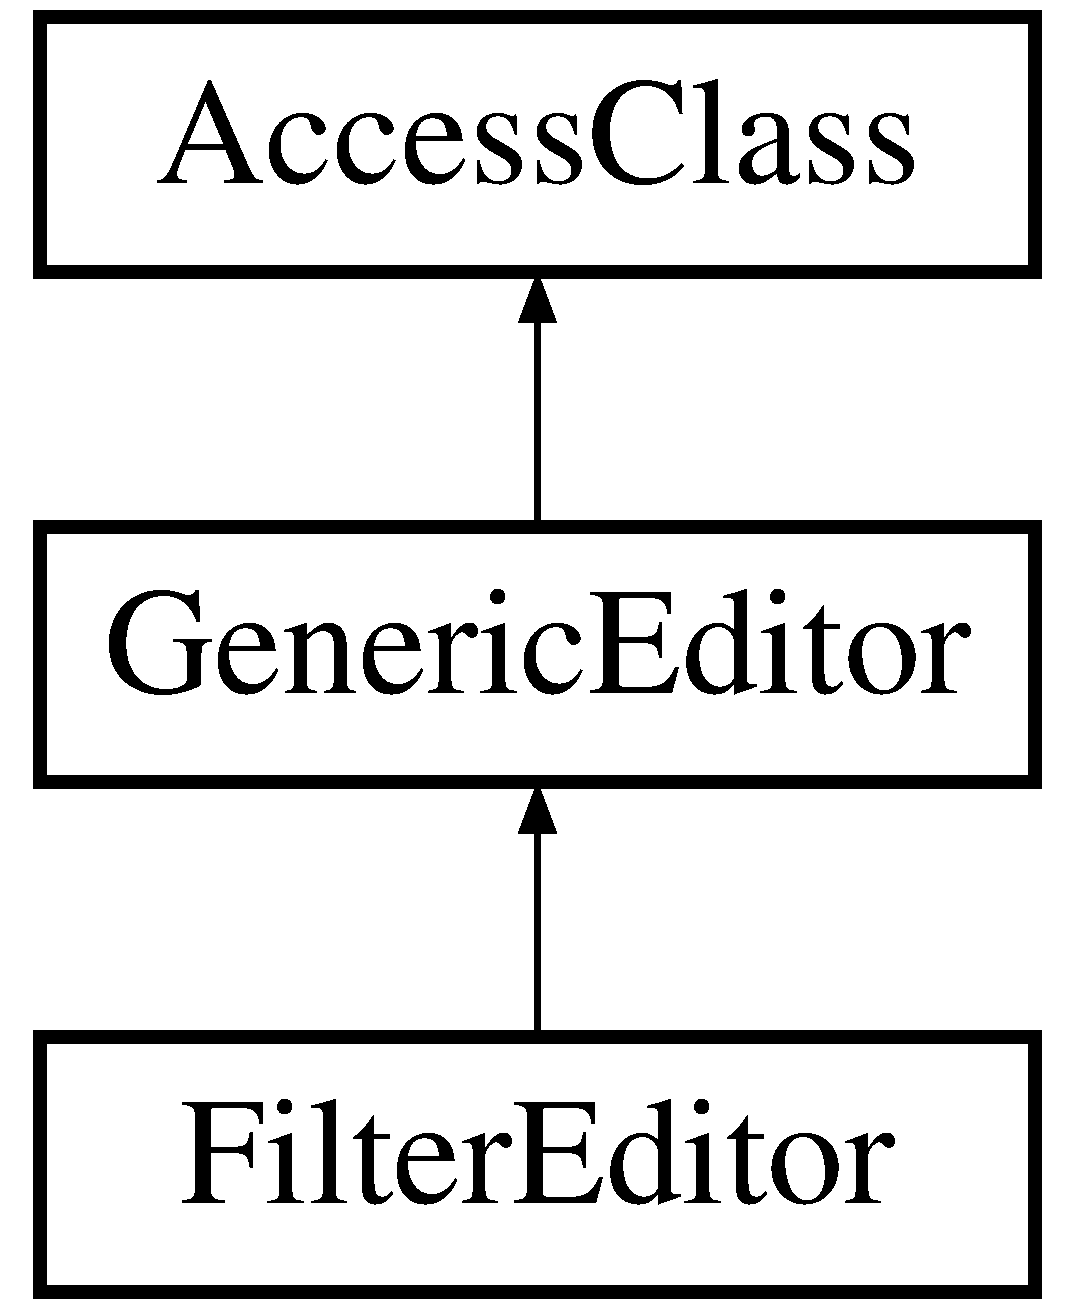
\includegraphics[height=3.000000cm]{classFilterEditor}
\end{center}
\end{figure}
\subsection*{Public Member Functions}
\begin{DoxyCompactItemize}
\item 
\hypertarget{classFilterEditor_a61c6bedbd0681fb649b4e1a302e05df7}{{\bfseries Filter\-Editor} (\hyperlink{classGenericProcessor}{Generic\-Processor} $\ast$parent\-Node)}\label{classFilterEditor_a61c6bedbd0681fb649b4e1a302e05df7}

\item 
\hypertarget{classFilterEditor_a79333a8d50202a3c9427a8e41d6457e9}{void {\bfseries button\-Event} (Button $\ast$button)}\label{classFilterEditor_a79333a8d50202a3c9427a8e41d6457e9}

\end{DoxyCompactItemize}
\subsection*{Private Member Functions}
\begin{DoxyCompactItemize}
\item 
\hypertarget{classFilterEditor_ad455b4ba047404a7d611429e26ea1a11}{{\bfseries J\-U\-C\-E\-\_\-\-D\-E\-C\-L\-A\-R\-E\-\_\-\-N\-O\-N\-\_\-\-C\-O\-P\-Y\-A\-B\-L\-E\-\_\-\-W\-I\-T\-H\-\_\-\-L\-E\-A\-K\-\_\-\-D\-E\-T\-E\-C\-T\-O\-R} (\hyperlink{classFilterEditor}{Filter\-Editor})}\label{classFilterEditor_ad455b4ba047404a7d611429e26ea1a11}

\end{DoxyCompactItemize}
\subsection*{Additional Inherited Members}


The documentation for this class was generated from the following file\-:\begin{DoxyCompactItemize}
\item 
Processors/\-Editors/Filter\-Editor.\-h\end{DoxyCompactItemize}

\hypertarget{classFilterNode}{\section{Filter\-Node Class Reference}
\label{classFilterNode}\index{Filter\-Node@{Filter\-Node}}
}


{\ttfamily \#include $<$Filter\-Node.\-h$>$}

Inheritance diagram for Filter\-Node\-:\begin{figure}[H]
\begin{center}
\leavevmode
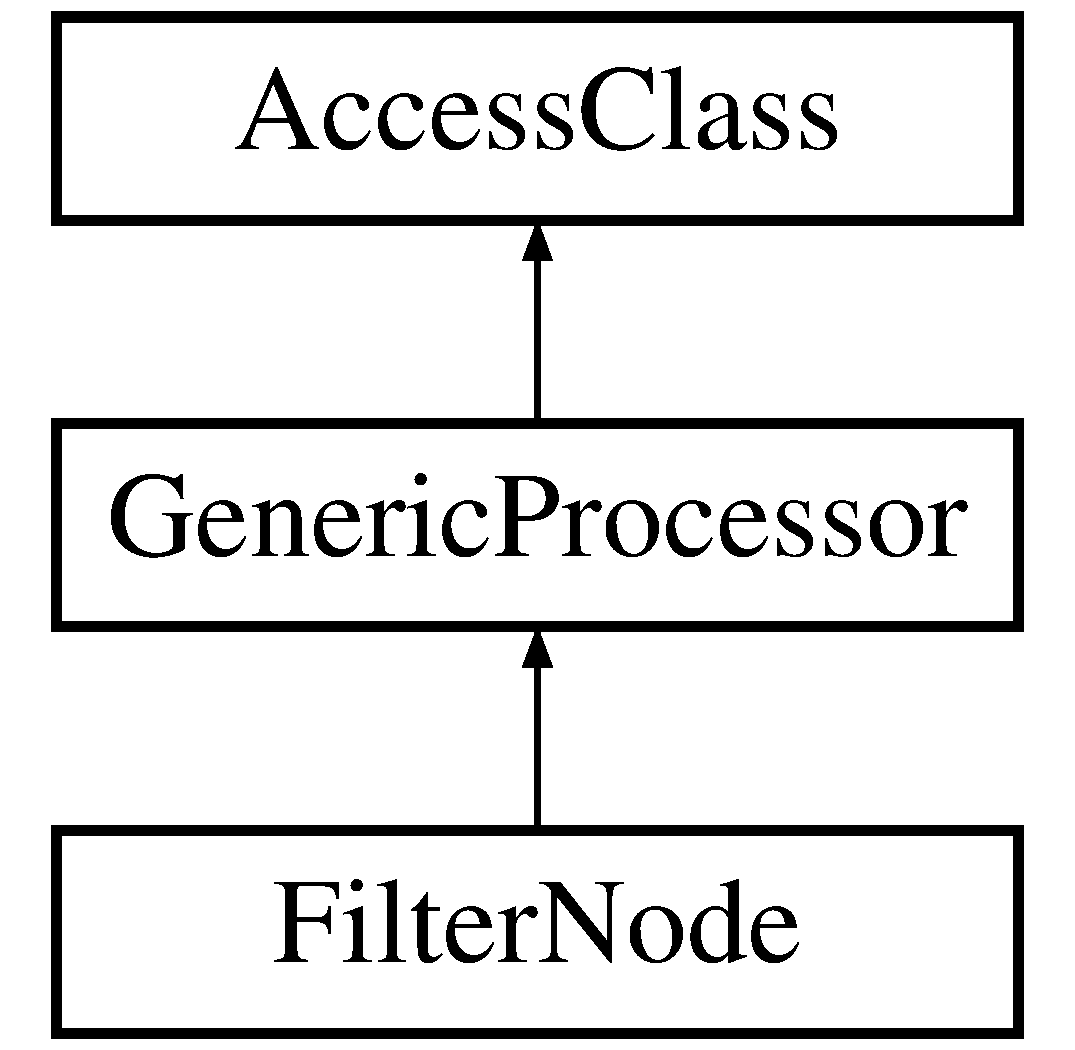
\includegraphics[height=3.000000cm]{classFilterNode}
\end{center}
\end{figure}
\subsection*{Public Member Functions}
\begin{DoxyCompactItemize}
\item 
\hypertarget{classFilterNode_a63dfa678d13ca12217d95a5b24475bfa}{void {\bfseries process} (Audio\-Sample\-Buffer \&buffer, Midi\-Buffer \&midi\-Messages, int \&n\-Samples)}\label{classFilterNode_a63dfa678d13ca12217d95a5b24475bfa}

\item 
\hypertarget{classFilterNode_a6369ae48f9ef18561a65027935a73e56}{void {\bfseries set\-Parameter} (int parameter\-Index, float new\-Value)}\label{classFilterNode_a6369ae48f9ef18561a65027935a73e56}

\item 
\hypertarget{classFilterNode_addd663abb4043bdb7296a63b93c49b85}{Audio\-Processor\-Editor $\ast$ {\bfseries create\-Editor} ()}\label{classFilterNode_addd663abb4043bdb7296a63b93c49b85}

\item 
\hypertarget{classFilterNode_aebf922de468ace2f70f09a7364e68649}{bool {\bfseries has\-Editor} () const }\label{classFilterNode_aebf922de468ace2f70f09a7364e68649}

\item 
\hypertarget{classFilterNode_aa009e8b04082517e15f17bcefc2ba497}{void {\bfseries update\-Settings} ()}\label{classFilterNode_aa009e8b04082517e15f17bcefc2ba497}

\end{DoxyCompactItemize}
\subsection*{Private Member Functions}
\begin{DoxyCompactItemize}
\item 
\hypertarget{classFilterNode_acbad7bee784f6b0f8704a625463689fc}{void {\bfseries set\-Filter\-Parameters} (double, double, int)}\label{classFilterNode_acbad7bee784f6b0f8704a625463689fc}

\item 
\hypertarget{classFilterNode_a119367d974155d2a2e03ac95600840aa}{{\bfseries J\-U\-C\-E\-\_\-\-D\-E\-C\-L\-A\-R\-E\-\_\-\-N\-O\-N\-\_\-\-C\-O\-P\-Y\-A\-B\-L\-E\-\_\-\-W\-I\-T\-H\-\_\-\-L\-E\-A\-K\-\_\-\-D\-E\-T\-E\-C\-T\-O\-R} (\hyperlink{classFilterNode}{Filter\-Node})}\label{classFilterNode_a119367d974155d2a2e03ac95600840aa}

\end{DoxyCompactItemize}
\subsection*{Private Attributes}
\begin{DoxyCompactItemize}
\item 
\hypertarget{classFilterNode_a15964c108a5c13314f1db847eb393ae8}{Array$<$ double $>$ {\bfseries low\-Cuts}}\label{classFilterNode_a15964c108a5c13314f1db847eb393ae8}

\item 
\hypertarget{classFilterNode_a66bef50d236e643a4db0a5249a799431}{Array$<$ double $>$ {\bfseries high\-Cuts}}\label{classFilterNode_a66bef50d236e643a4db0a5249a799431}

\item 
\hypertarget{classFilterNode_ae3c8b408bdc08a967069c3918c2314c3}{Owned\-Array$<$ Dsp\-::\-Filter $>$ {\bfseries filters}}\label{classFilterNode_ae3c8b408bdc08a967069c3918c2314c3}

\end{DoxyCompactItemize}
\subsection*{Additional Inherited Members}


\subsection{Detailed Description}
Filters data using a filter from the D\-S\-P library.

The user can select the low-\/ and high-\/frequency cutoffs.

\begin{DoxySeeAlso}{See also}
\hyperlink{classGenericProcessor}{Generic\-Processor}, \hyperlink{classFilterEditor}{Filter\-Editor} 
\end{DoxySeeAlso}


The documentation for this class was generated from the following file\-:\begin{DoxyCompactItemize}
\item 
Processors/Filter\-Node.\-h\end{DoxyCompactItemize}

\hypertarget{classFPGAThread}{\section{F\-P\-G\-A\-Thread Class Reference}
\label{classFPGAThread}\index{F\-P\-G\-A\-Thread@{F\-P\-G\-A\-Thread}}
}
Inheritance diagram for F\-P\-G\-A\-Thread\-:\begin{figure}[H]
\begin{center}
\leavevmode
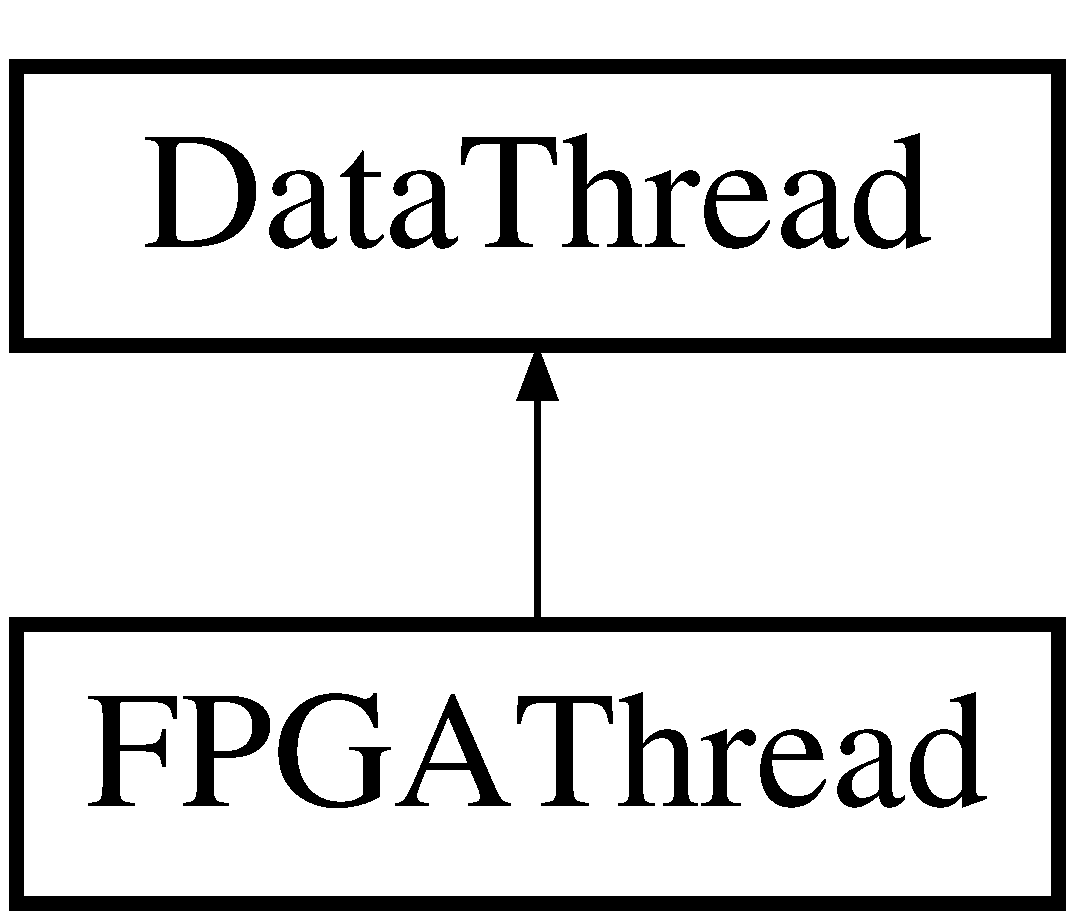
\includegraphics[height=2.000000cm]{classFPGAThread}
\end{center}
\end{figure}
\subsection*{Public Member Functions}
\begin{DoxyCompactItemize}
\item 
\hypertarget{classFPGAThread_a3a5d5862b45dfde64caf30c6b173fcea}{{\bfseries F\-P\-G\-A\-Thread} (\hyperlink{classSourceNode}{Source\-Node} $\ast$sn)}\label{classFPGAThread_a3a5d5862b45dfde64caf30c6b173fcea}

\item 
\hypertarget{classFPGAThread_a58958c632739119e57126ceaf7ae9210}{bool {\bfseries found\-Input\-Source} ()}\label{classFPGAThread_a58958c632739119e57126ceaf7ae9210}

\item 
\hypertarget{classFPGAThread_a67ff95c727afa4c92d9705c3b1d9c3ee}{int {\bfseries get\-Num\-Channels} ()}\label{classFPGAThread_a67ff95c727afa4c92d9705c3b1d9c3ee}

\item 
\hypertarget{classFPGAThread_a8d1bd558f7e72a8f578db63736df22cf}{float {\bfseries get\-Sample\-Rate} ()}\label{classFPGAThread_a8d1bd558f7e72a8f578db63736df22cf}

\item 
\hypertarget{classFPGAThread_a30096ea04ec85c0aa301f167fd7a42c4}{float {\bfseries get\-Bit\-Volts} ()}\label{classFPGAThread_a30096ea04ec85c0aa301f167fd7a42c4}

\end{DoxyCompactItemize}
\subsection*{Private Member Functions}
\begin{DoxyCompactItemize}
\item 
\hypertarget{classFPGAThread_ae60d0b8a8d6ce978040f9c0a0a613399}{bool {\bfseries initialize\-F\-P\-G\-A} (bool)}\label{classFPGAThread_ae60d0b8a8d6ce978040f9c0a0a613399}

\item 
\hypertarget{classFPGAThread_a26a37cd26819b8bf884d9607df7078e0}{bool {\bfseries close\-F\-P\-G\-A} ()}\label{classFPGAThread_a26a37cd26819b8bf884d9607df7078e0}

\item 
\hypertarget{classFPGAThread_a0b23746128abec94e4ed5ef1f7e6e115}{bool {\bfseries start\-Acquisition} ()}\label{classFPGAThread_a0b23746128abec94e4ed5ef1f7e6e115}

\item 
\hypertarget{classFPGAThread_a38a4c39dfbd30ef38bbcee3be29ebb65}{bool {\bfseries stop\-Acquisition} ()}\label{classFPGAThread_a38a4c39dfbd30ef38bbcee3be29ebb65}

\item 
\hypertarget{classFPGAThread_a2d4ea188b4d9f1f77affd5cc95debc5a}{bool {\bfseries update\-Buffer} ()}\label{classFPGAThread_a2d4ea188b4d9f1f77affd5cc95debc5a}

\item 
\hypertarget{classFPGAThread_aef8282fed618e89f9e5cd2c98bf28cb6}{{\bfseries J\-U\-C\-E\-\_\-\-D\-E\-C\-L\-A\-R\-E\-\_\-\-N\-O\-N\-\_\-\-C\-O\-P\-Y\-A\-B\-L\-E\-\_\-\-W\-I\-T\-H\-\_\-\-L\-E\-A\-K\-\_\-\-D\-E\-T\-E\-C\-T\-O\-R} (\hyperlink{classFPGAThread}{F\-P\-G\-A\-Thread})}\label{classFPGAThread_aef8282fed618e89f9e5cd2c98bf28cb6}

\end{DoxyCompactItemize}
\subsection*{Private Attributes}
\begin{DoxyCompactItemize}
\item 
\hypertarget{classFPGAThread_aefc8169fcf432084604e668bdd002e33}{ok\-C\-Front\-Panel $\ast$ {\bfseries dev}}\label{classFPGAThread_aefc8169fcf432084604e668bdd002e33}

\item 
\hypertarget{classFPGAThread_afcdaa6785c45d61e82dacace5271d148}{char {\bfseries bitfile} \mbox{[}128\mbox{]}}\label{classFPGAThread_afcdaa6785c45d61e82dacace5271d148}

\item 
\hypertarget{classFPGAThread_ad945f39bbd0160eb7671fc056698fc6f}{char {\bfseries dll\-\_\-date} \mbox{[}32\mbox{]}}\label{classFPGAThread_ad945f39bbd0160eb7671fc056698fc6f}

\item 
\hypertarget{classFPGAThread_a9d02817493e33881ef5850ebb42dce22}{char {\bfseries dll\-\_\-time} \mbox{[}32\mbox{]}}\label{classFPGAThread_a9d02817493e33881ef5850ebb42dce22}

\item 
\hypertarget{classFPGAThread_ad4248ed5641cb562fb70d80276e3c5a6}{bool {\bfseries is\-Transmitting}}\label{classFPGAThread_ad4248ed5641cb562fb70d80276e3c5a6}

\item 
\hypertarget{classFPGAThread_a3ee2a5e5baa7812c17f8005f6dd7fed0}{bool {\bfseries device\-Found}}\label{classFPGAThread_a3ee2a5e5baa7812c17f8005f6dd7fed0}

\item 
\hypertarget{classFPGAThread_a85e1ec77b3726177ec431524e1bd73bc}{unsigned char {\bfseries p\-Buffer} \mbox{[}50000\mbox{]}}\label{classFPGAThread_a85e1ec77b3726177ec431524e1bd73bc}

\item 
\hypertarget{classFPGAThread_a26b6ea54b00046051beb3ab6d0d28181}{float {\bfseries this\-Sample} \mbox{[}32\mbox{]}}\label{classFPGAThread_a26b6ea54b00046051beb3ab6d0d28181}

\item 
\hypertarget{classFPGAThread_a076e7ac64107a0a51a6623e278a81914}{int {\bfseries numchannels}}\label{classFPGAThread_a076e7ac64107a0a51a6623e278a81914}

\item 
\hypertarget{classFPGAThread_a7d3d6dd86acd3f747ed60c88d133aa15}{int {\bfseries Ndatabytes}}\label{classFPGAThread_a7d3d6dd86acd3f747ed60c88d133aa15}

\end{DoxyCompactItemize}
\subsection*{Additional Inherited Members}


The documentation for this class was generated from the following file\-:\begin{DoxyCompactItemize}
\item 
Processors/\-Data\-Threads/F\-P\-G\-A\-Thread.\-h\end{DoxyCompactItemize}

\hypertarget{classGenericAxes}{\section{Generic\-Axes Class Reference}
\label{classGenericAxes}\index{Generic\-Axes@{Generic\-Axes}}
}
Inheritance diagram for Generic\-Axes\-:\begin{figure}[H]
\begin{center}
\leavevmode
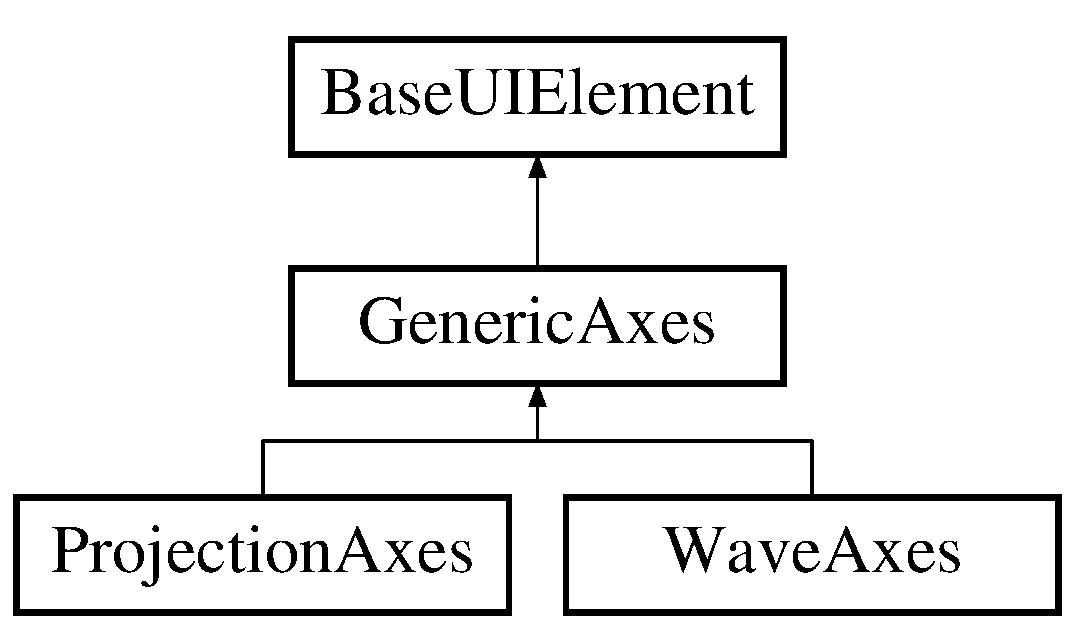
\includegraphics[height=3.000000cm]{classGenericAxes}
\end{center}
\end{figure}
\subsection*{Public Member Functions}
\begin{DoxyCompactItemize}
\item 
\hypertarget{classGenericAxes_a815be990a5475cb83b0c576beb79b4b8}{{\bfseries Generic\-Axes} (int x, int y, double w, double h, int t)}\label{classGenericAxes_a815be990a5475cb83b0c576beb79b4b8}

\item 
\hypertarget{classGenericAxes_ae44757d835ffd6de1c4fa05d57b77220}{void {\bfseries update\-Spike\-Data} (\hyperlink{structSpikeObject}{Spike\-Object} s)}\label{classGenericAxes_ae44757d835ffd6de1c4fa05d57b77220}

\item 
\hypertarget{classGenericAxes_ada612f54fc4e1354e2c356b0b0b713ab}{virtual void {\bfseries redraw} ()}\label{classGenericAxes_ada612f54fc4e1354e2c356b0b0b713ab}

\item 
\hypertarget{classGenericAxes_a4a2a5bb51f6c77d63fa8a6dec43b59c3}{void {\bfseries set\-X\-Lims} (double xmin, double xmax)}\label{classGenericAxes_a4a2a5bb51f6c77d63fa8a6dec43b59c3}

\item 
\hypertarget{classGenericAxes_a42f93ea776da8f543a5afaa932ee5f79}{void {\bfseries get\-X\-Lims} (double $\ast$xmin, double $\ast$xmax)}\label{classGenericAxes_a42f93ea776da8f543a5afaa932ee5f79}

\item 
\hypertarget{classGenericAxes_a5e9a75eaa20902a27b493e09cd567bcf}{void {\bfseries set\-Y\-Lims} (double ymin, double ymax)}\label{classGenericAxes_a5e9a75eaa20902a27b493e09cd567bcf}

\item 
\hypertarget{classGenericAxes_a6b81438346cb943333ad3113b1c07db2}{void {\bfseries get\-Y\-Lims} (double $\ast$ymin, double $\ast$ymax)}\label{classGenericAxes_a6b81438346cb943333ad3113b1c07db2}

\item 
\hypertarget{classGenericAxes_a7efbbf40fea1e85867a63af8cbdc2caf}{void {\bfseries set\-Type} (int type)}\label{classGenericAxes_a7efbbf40fea1e85867a63af8cbdc2caf}

\item 
\hypertarget{classGenericAxes_afd15d28941f474a93e625832b560bec7}{int {\bfseries get\-Type} ()}\label{classGenericAxes_afd15d28941f474a93e625832b560bec7}

\item 
\hypertarget{classGenericAxes_a41bf0d084d8bb593369fd3fef2067cf7}{void {\bfseries set\-Position} (int, int, double, double)}\label{classGenericAxes_a41bf0d084d8bb593369fd3fef2067cf7}

\end{DoxyCompactItemize}
\subsection*{Protected Member Functions}
\begin{DoxyCompactItemize}
\item 
\hypertarget{classGenericAxes_ab8efb505a6c8286afb705337cec42861}{virtual void {\bfseries plot} ()}\label{classGenericAxes_ab8efb505a6c8286afb705337cec42861}

\item 
\hypertarget{classGenericAxes_a6d73141222a531855a768646f05e79e6}{void {\bfseries load\-Font} ()}\label{classGenericAxes_a6d73141222a531855a768646f05e79e6}

\end{DoxyCompactItemize}
\subsection*{Protected Attributes}
\begin{DoxyCompactItemize}
\item 
\hypertarget{classGenericAxes_a0dc6ef82871c7cc4e9c314b554906e8d}{double {\bfseries xlims} \mbox{[}2\mbox{]}}\label{classGenericAxes_a0dc6ef82871c7cc4e9c314b554906e8d}

\item 
\hypertarget{classGenericAxes_a36cc6558d5be963c0ca0808692e297fe}{double {\bfseries ylims} \mbox{[}2\mbox{]}}\label{classGenericAxes_a36cc6558d5be963c0ca0808692e297fe}

\item 
\hypertarget{classGenericAxes_a693c35b3105a60b704e3cac87b376188}{\hyperlink{structSpikeObject}{Spike\-Object} {\bfseries s}}\label{classGenericAxes_a693c35b3105a60b704e3cac87b376188}

\item 
\hypertarget{classGenericAxes_aa9da8940de6ecf1e6f7816b3186d9470}{bool {\bfseries got\-First\-Spike}}\label{classGenericAxes_aa9da8940de6ecf1e6f7816b3186d9470}

\item 
\hypertarget{classGenericAxes_a0550968e57ded25fa92c7e4108efe904}{int {\bfseries type}}\label{classGenericAxes_a0550968e57ded25fa92c7e4108efe904}

\item 
\hypertarget{classGenericAxes_a511911db715747218e92832b482a76a8}{F\-T\-Pixmap\-Font $\ast$ {\bfseries font}}\label{classGenericAxes_a511911db715747218e92832b482a76a8}

\end{DoxyCompactItemize}


The documentation for this class was generated from the following file\-:\begin{DoxyCompactItemize}
\item 
Processors/\-Visualization/\-Spike\-Plotting/Generic\-Axes.\-h\end{DoxyCompactItemize}

\hypertarget{classGenericEditor}{\section{Generic\-Editor Class Reference}
\label{classGenericEditor}\index{Generic\-Editor@{Generic\-Editor}}
}
Inheritance diagram for Generic\-Editor\-:\begin{figure}[H]
\begin{center}
\leavevmode
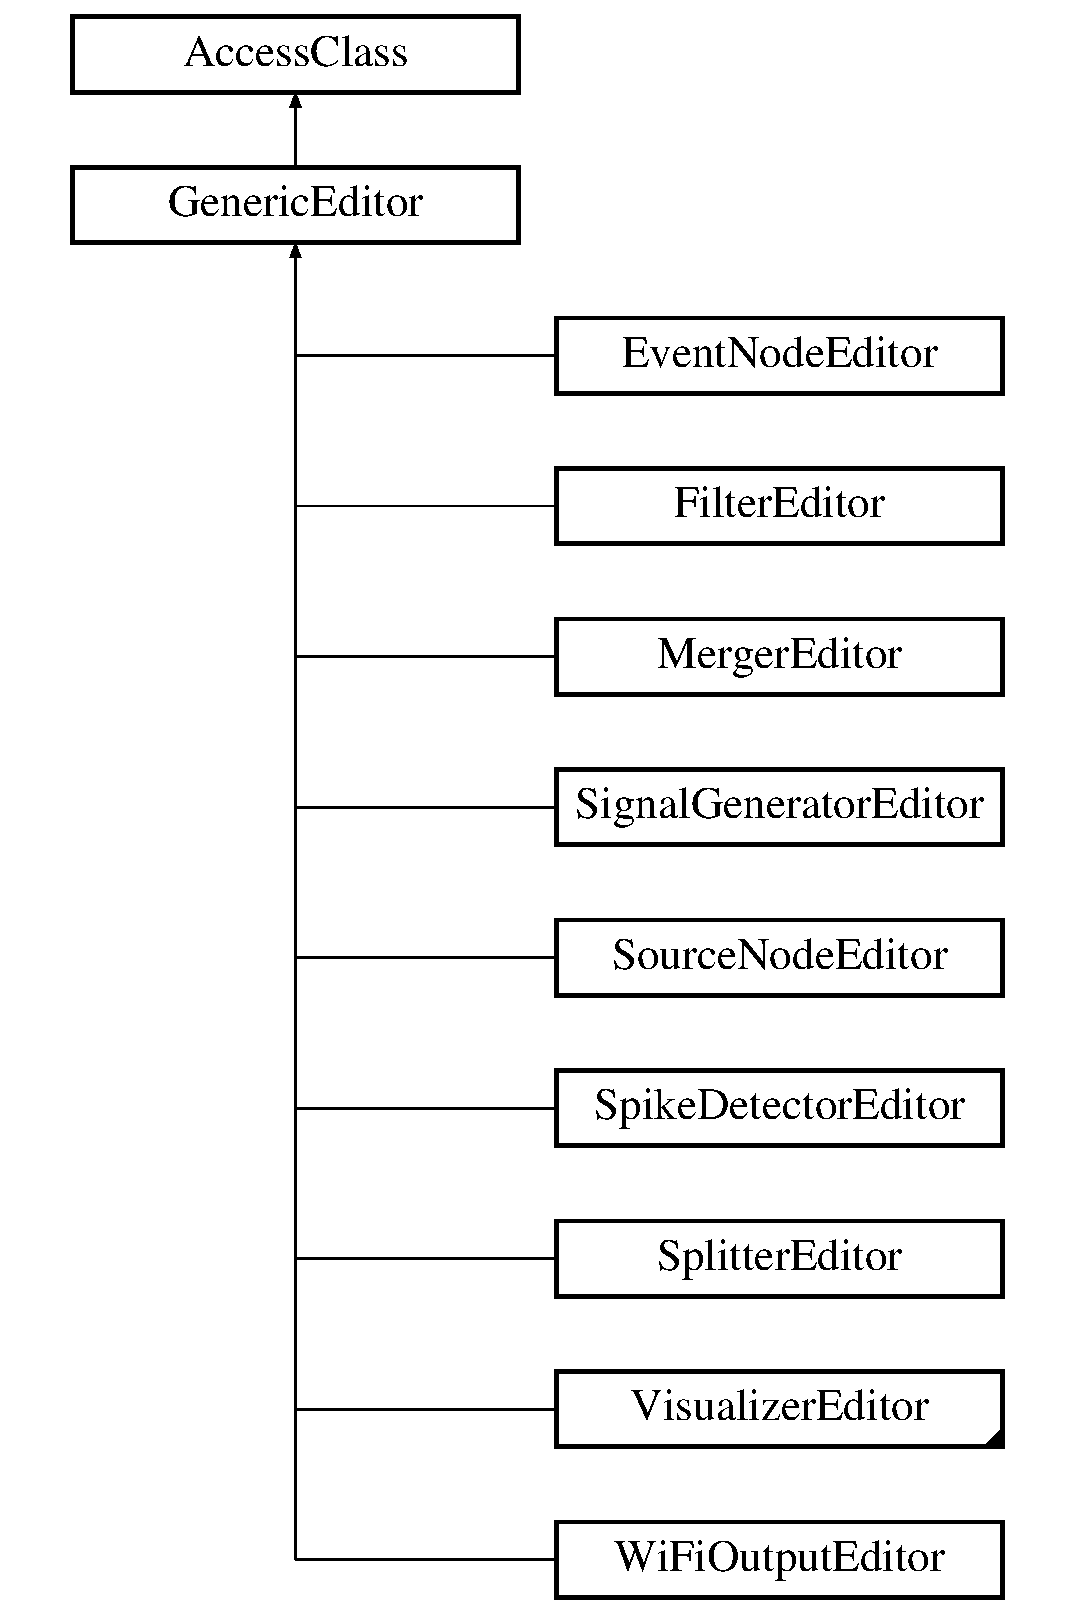
\includegraphics[height=11.000000cm]{classGenericEditor}
\end{center}
\end{figure}
\subsection*{Public Member Functions}
\begin{DoxyCompactItemize}
\item 
\hypertarget{classGenericEditor_a2e9634ca6753f1f4729cb8cc1b1e1757}{{\bfseries Generic\-Editor} (\hyperlink{classGenericProcessor}{Generic\-Processor} $\ast$owner)}\label{classGenericEditor_a2e9634ca6753f1f4729cb8cc1b1e1757}

\item 
\hypertarget{classGenericEditor_a6da2cb554793f7c24919ca0d3a860807}{void {\bfseries paint} (Graphics \&g)}\label{classGenericEditor_a6da2cb554793f7c24919ca0d3a860807}

\item 
\hypertarget{classGenericEditor_a1d95f3fa72eff3aca781736951052dd9}{bool {\bfseries key\-Pressed} (const Key\-Press \&key)}\label{classGenericEditor_a1d95f3fa72eff3aca781736951052dd9}

\item 
\hypertarget{classGenericEditor_adf3039a522fd423bb090ab31041748fe}{void {\bfseries switch\-Selected\-State} ()}\label{classGenericEditor_adf3039a522fd423bb090ab31041748fe}

\item 
\hypertarget{classGenericEditor_a6b2fc0a74e858b94cefa70fd6c2dfbf9}{void {\bfseries select} ()}\label{classGenericEditor_a6b2fc0a74e858b94cefa70fd6c2dfbf9}

\item 
\hypertarget{classGenericEditor_a0d24085ae8fd1b230c028495f47f5d33}{void {\bfseries highlight} ()}\label{classGenericEditor_a0d24085ae8fd1b230c028495f47f5d33}

\item 
\hypertarget{classGenericEditor_ab81335b8bae46480ffbfc6d3a049ce76}{void {\bfseries deselect} ()}\label{classGenericEditor_ab81335b8bae46480ffbfc6d3a049ce76}

\item 
\hypertarget{classGenericEditor_af8c36ade567c70457ff8b9034ed3a5a0}{bool {\bfseries get\-Selection\-State} ()}\label{classGenericEditor_af8c36ade567c70457ff8b9034ed3a5a0}

\item 
\hypertarget{classGenericEditor_a5218e677eba574ad85c70004ff4ef089}{void {\bfseries enable} ()}\label{classGenericEditor_a5218e677eba574ad85c70004ff4ef089}

\item 
\hypertarget{classGenericEditor_a03f6eb4b700a70d1b9c93353105430cf}{void {\bfseries disable} ()}\label{classGenericEditor_a03f6eb4b700a70d1b9c93353105430cf}

\item 
\hypertarget{classGenericEditor_aaf58e7b9b61880c663f1ae893795536d}{bool {\bfseries get\-Enabled\-State} ()}\label{classGenericEditor_aaf58e7b9b61880c663f1ae893795536d}

\item 
\hypertarget{classGenericEditor_a4f3cc622bce35efefa9e40dc7514e8cb}{void {\bfseries set\-Enabled\-State} (bool)}\label{classGenericEditor_a4f3cc622bce35efefa9e40dc7514e8cb}

\item 
\hypertarget{classGenericEditor_a4f4d9db286b2518197a3b96ec1b0c754}{String {\bfseries get\-Name} ()}\label{classGenericEditor_a4f4d9db286b2518197a3b96ec1b0c754}

\item 
\hypertarget{classGenericEditor_afc1b81bb8204c4caf1bf20197fa9fd5a}{virtual void {\bfseries tab\-Number} (int t)}\label{classGenericEditor_afc1b81bb8204c4caf1bf20197fa9fd5a}

\item 
\hypertarget{classGenericEditor_a505b9b2710a39cdeb7645e3316331167}{int {\bfseries tab\-Number} ()}\label{classGenericEditor_a505b9b2710a39cdeb7645e3316331167}

\item 
\hypertarget{classGenericEditor_a3fd6b67a679044960a2c702ecff9e978}{virtual void {\bfseries switch\-Source} (int)}\label{classGenericEditor_a3fd6b67a679044960a2c702ecff9e978}

\item 
\hypertarget{classGenericEditor_a5660d57f3a50a580a78c5da7ebaa5052}{virtual void {\bfseries switch\-Source} ()}\label{classGenericEditor_a5660d57f3a50a580a78c5da7ebaa5052}

\item 
\hypertarget{classGenericEditor_a78be9c8932e8b069861ffe5b5933ece2}{\hyperlink{classGenericProcessor}{Generic\-Processor} $\ast$ {\bfseries get\-Processor} () const }\label{classGenericEditor_a78be9c8932e8b069861ffe5b5933ece2}

\item 
\hypertarget{classGenericEditor_af0234d4371dfe907e0654b9d68902644}{void {\bfseries fade\-In} ()}\label{classGenericEditor_af0234d4371dfe907e0654b9d68902644}

\item 
\hypertarget{classGenericEditor_a4185563e9254688df9bf552d2e5d2cec}{virtual void {\bfseries switch\-Dest} ()}\label{classGenericEditor_a4185563e9254688df9bf552d2e5d2cec}

\item 
\hypertarget{classGenericEditor_acd818101b35bd11e9d2399397a7c6ce7}{virtual void {\bfseries switch\-I\-O} (int)}\label{classGenericEditor_acd818101b35bd11e9d2399397a7c6ce7}

\item 
\hypertarget{classGenericEditor_a173791183751d6d59a82d56bf1e76073}{virtual void {\bfseries button\-Clicked} (Button $\ast$button)}\label{classGenericEditor_a173791183751d6d59a82d56bf1e76073}

\item 
\hypertarget{classGenericEditor_a83ae83a2c671317b4f4e07265c76aced}{virtual void {\bfseries button\-Event} (Button $\ast$button)}\label{classGenericEditor_a83ae83a2c671317b4f4e07265c76aced}

\item 
\hypertarget{classGenericEditor_aba93f26ee969aa06a78e723378a175ad}{virtual void {\bfseries slider\-Value\-Changed} (Slider $\ast$slider)}\label{classGenericEditor_aba93f26ee969aa06a78e723378a175ad}

\item 
\hypertarget{classGenericEditor_a0d8e6f21e173e9ab2588ee69b94483b0}{virtual void {\bfseries slider\-Event} (Slider $\ast$slider)}\label{classGenericEditor_a0d8e6f21e173e9ab2588ee69b94483b0}

\item 
\hypertarget{classGenericEditor_a255d76cc78f46761e10d65523512f306}{virtual void {\bfseries editor\-Was\-Clicked} ()}\label{classGenericEditor_a255d76cc78f46761e10d65523512f306}

\item 
\hypertarget{classGenericEditor_ac25d5d6e473cf8c8dde7490e5008c4fb}{bool {\bfseries check\-Drawer\-Button} (Button $\ast$button)}\label{classGenericEditor_ac25d5d6e473cf8c8dde7490e5008c4fb}

\item 
\hypertarget{classGenericEditor_a506f7e0099f41148a4a930f19eb9a13c}{bool {\bfseries get\-Record\-Status} (int chan)}\label{classGenericEditor_a506f7e0099f41148a4a930f19eb9a13c}

\item 
\hypertarget{classGenericEditor_a3b176ac12dd5f498630ee131be1338f3}{bool {\bfseries get\-Audio\-Status} (int chan)}\label{classGenericEditor_a3b176ac12dd5f498630ee131be1338f3}

\item 
\hypertarget{classGenericEditor_a2a60858cac03995dc95a77fef58de214}{void {\bfseries select\-Channels} (Array$<$ int $>$)}\label{classGenericEditor_a2a60858cac03995dc95a77fef58de214}

\item 
\hypertarget{classGenericEditor_acc0898d4f9b1c5850e89967150bb3711}{void {\bfseries refresh\-Colors} ()}\label{classGenericEditor_acc0898d4f9b1c5850e89967150bb3711}

\item 
\hypertarget{classGenericEditor_a571efb4db3a66c9e4622c16de2459e46}{virtual void {\bfseries update} ()}\label{classGenericEditor_a571efb4db3a66c9e4622c16de2459e46}

\item 
\hypertarget{classGenericEditor_aebe91d40297fc4dfe6c1b783811f1d2c}{virtual void {\bfseries update\-Settings} ()}\label{classGenericEditor_aebe91d40297fc4dfe6c1b783811f1d2c}

\item 
\hypertarget{classGenericEditor_ad3c5b85a9ae515780e1aaeb2c1128ef4}{virtual void {\bfseries update\-Visualizer} ()}\label{classGenericEditor_ad3c5b85a9ae515780e1aaeb2c1128ef4}

\item 
\hypertarget{classGenericEditor_a61e0bb3378d87a69ad58a487d34afd70}{virtual void {\bfseries channel\-Changed} (int chan)}\label{classGenericEditor_a61e0bb3378d87a69ad58a487d34afd70}

\item 
\hypertarget{classGenericEditor_a42a9df2a674bbbf9dfa3ed221aa43e4a}{Array$<$ int $>$ {\bfseries get\-Active\-Channels} ()}\label{classGenericEditor_a42a9df2a674bbbf9dfa3ed221aa43e4a}

\item 
\hypertarget{classGenericEditor_ada6b7835cbd9b2170b5dc46316068978}{int {\bfseries get\-Start\-Channel} ()}\label{classGenericEditor_ada6b7835cbd9b2170b5dc46316068978}

\end{DoxyCompactItemize}
\subsection*{Public Attributes}
\begin{DoxyCompactItemize}
\item 
\hypertarget{classGenericEditor_ab5b6f3450c9376c313fe8925bfbe4bc9}{int {\bfseries desired\-Width}}\label{classGenericEditor_ab5b6f3450c9376c313fe8925bfbe4bc9}

\item 
\hypertarget{classGenericEditor_a53166218592772efb4f6ef664ec4763b}{int {\bfseries node\-Id}}\label{classGenericEditor_a53166218592772efb4f6ef664ec4763b}

\item 
\hypertarget{classGenericEditor_af961769014471610d0eeeeefb8e712ef}{bool {\bfseries is\-Fading}}\label{classGenericEditor_af961769014471610d0eeeeefb8e712ef}

\item 
\hypertarget{classGenericEditor_ab4430a824b8ea6f3d3bd55ef037c40d2}{float {\bfseries accumulator}}\label{classGenericEditor_ab4430a824b8ea6f3d3bd55ef037c40d2}

\item 
\hypertarget{classGenericEditor_ac544d3401113c612bf992feacc68d961}{Font {\bfseries title\-Font}}\label{classGenericEditor_ac544d3401113c612bf992feacc68d961}

\end{DoxyCompactItemize}
\subsection*{Protected Member Functions}
\begin{DoxyCompactItemize}
\item 
\hypertarget{classGenericEditor_aace3206666ab83eb3f89d604bbe1998f}{virtual void {\bfseries add\-Parameter\-Editors} ()}\label{classGenericEditor_aace3206666ab83eb3f89d604bbe1998f}

\end{DoxyCompactItemize}
\subsection*{Protected Attributes}
\begin{DoxyCompactItemize}
\item 
\hypertarget{classGenericEditor_afb5e6e83bf76e18fb0d3d2b1d75ee8b5}{\hyperlink{classDrawerButton}{Drawer\-Button} $\ast$ {\bfseries drawer\-Button}}\label{classGenericEditor_afb5e6e83bf76e18fb0d3d2b1d75ee8b5}

\item 
\hypertarget{classGenericEditor_a4f24167f68b01041cebdcb15d161432d}{int {\bfseries drawer\-Width}}\label{classGenericEditor_a4f24167f68b01041cebdcb15d161432d}

\item 
\hypertarget{classGenericEditor_ab8a5e6c65cf62c23e9a9b2856c9b78f9}{\hyperlink{classChannelSelector}{Channel\-Selector} $\ast$ {\bfseries channel\-Selector}}\label{classGenericEditor_ab8a5e6c65cf62c23e9a9b2856c9b78f9}

\end{DoxyCompactItemize}
\subsection*{Private Member Functions}
\begin{DoxyCompactItemize}
\item 
\hypertarget{classGenericEditor_a12c45104009fc083007c65f040583320}{virtual void {\bfseries timer\-Callback} ()}\label{classGenericEditor_a12c45104009fc083007c65f040583320}

\item 
\hypertarget{classGenericEditor_aab1e9c4f507c32cd1683a4fd2b610718}{virtual void {\bfseries resized} ()}\label{classGenericEditor_aab1e9c4f507c32cd1683a4fd2b610718}

\item 
\hypertarget{classGenericEditor_a4deed1f9dcc59fb630d0ca0a5d62b5ab}{{\bfseries J\-U\-C\-E\-\_\-\-D\-E\-C\-L\-A\-R\-E\-\_\-\-N\-O\-N\-\_\-\-C\-O\-P\-Y\-A\-B\-L\-E\-\_\-\-W\-I\-T\-H\-\_\-\-L\-E\-A\-K\-\_\-\-D\-E\-T\-E\-C\-T\-O\-R} (\hyperlink{classGenericEditor}{Generic\-Editor})}\label{classGenericEditor_a4deed1f9dcc59fb630d0ca0a5d62b5ab}

\end{DoxyCompactItemize}
\subsection*{Private Attributes}
\begin{DoxyCompactItemize}
\item 
\hypertarget{classGenericEditor_a0763036019394e15cc49ab1bffb57333}{Colour {\bfseries background\-Color}}\label{classGenericEditor_a0763036019394e15cc49ab1bffb57333}

\item 
\hypertarget{classGenericEditor_adfb224e3a4b76277d020172fa837c334}{Colour\-Gradient {\bfseries background\-Gradient}}\label{classGenericEditor_adfb224e3a4b76277d020172fa837c334}

\item 
\hypertarget{classGenericEditor_aee0ece43c57ee21df782e481fc8e8959}{bool {\bfseries is\-Selected}}\label{classGenericEditor_aee0ece43c57ee21df782e481fc8e8959}

\item 
\hypertarget{classGenericEditor_a2481dbae00beaed730efcaa00e6d8e92}{bool {\bfseries is\-Enabled}}\label{classGenericEditor_a2481dbae00beaed730efcaa00e6d8e92}

\item 
\hypertarget{classGenericEditor_aa6ac3f1214a6e746a04293b2a17f5912}{int {\bfseries t\-Num}}\label{classGenericEditor_aa6ac3f1214a6e746a04293b2a17f5912}

\item 
\hypertarget{classGenericEditor_a7e0e6439c13dbea6863e0f4c9468700c}{String {\bfseries name}}\label{classGenericEditor_a7e0e6439c13dbea6863e0f4c9468700c}

\end{DoxyCompactItemize}


The documentation for this class was generated from the following file\-:\begin{DoxyCompactItemize}
\item 
Processors/\-Editors/Generic\-Editor.\-h\end{DoxyCompactItemize}

\hypertarget{classGenericProcessor}{\section{Generic\-Processor Class Reference}
\label{classGenericProcessor}\index{Generic\-Processor@{Generic\-Processor}}
}
Inheritance diagram for Generic\-Processor\-:\begin{figure}[H]
\begin{center}
\leavevmode
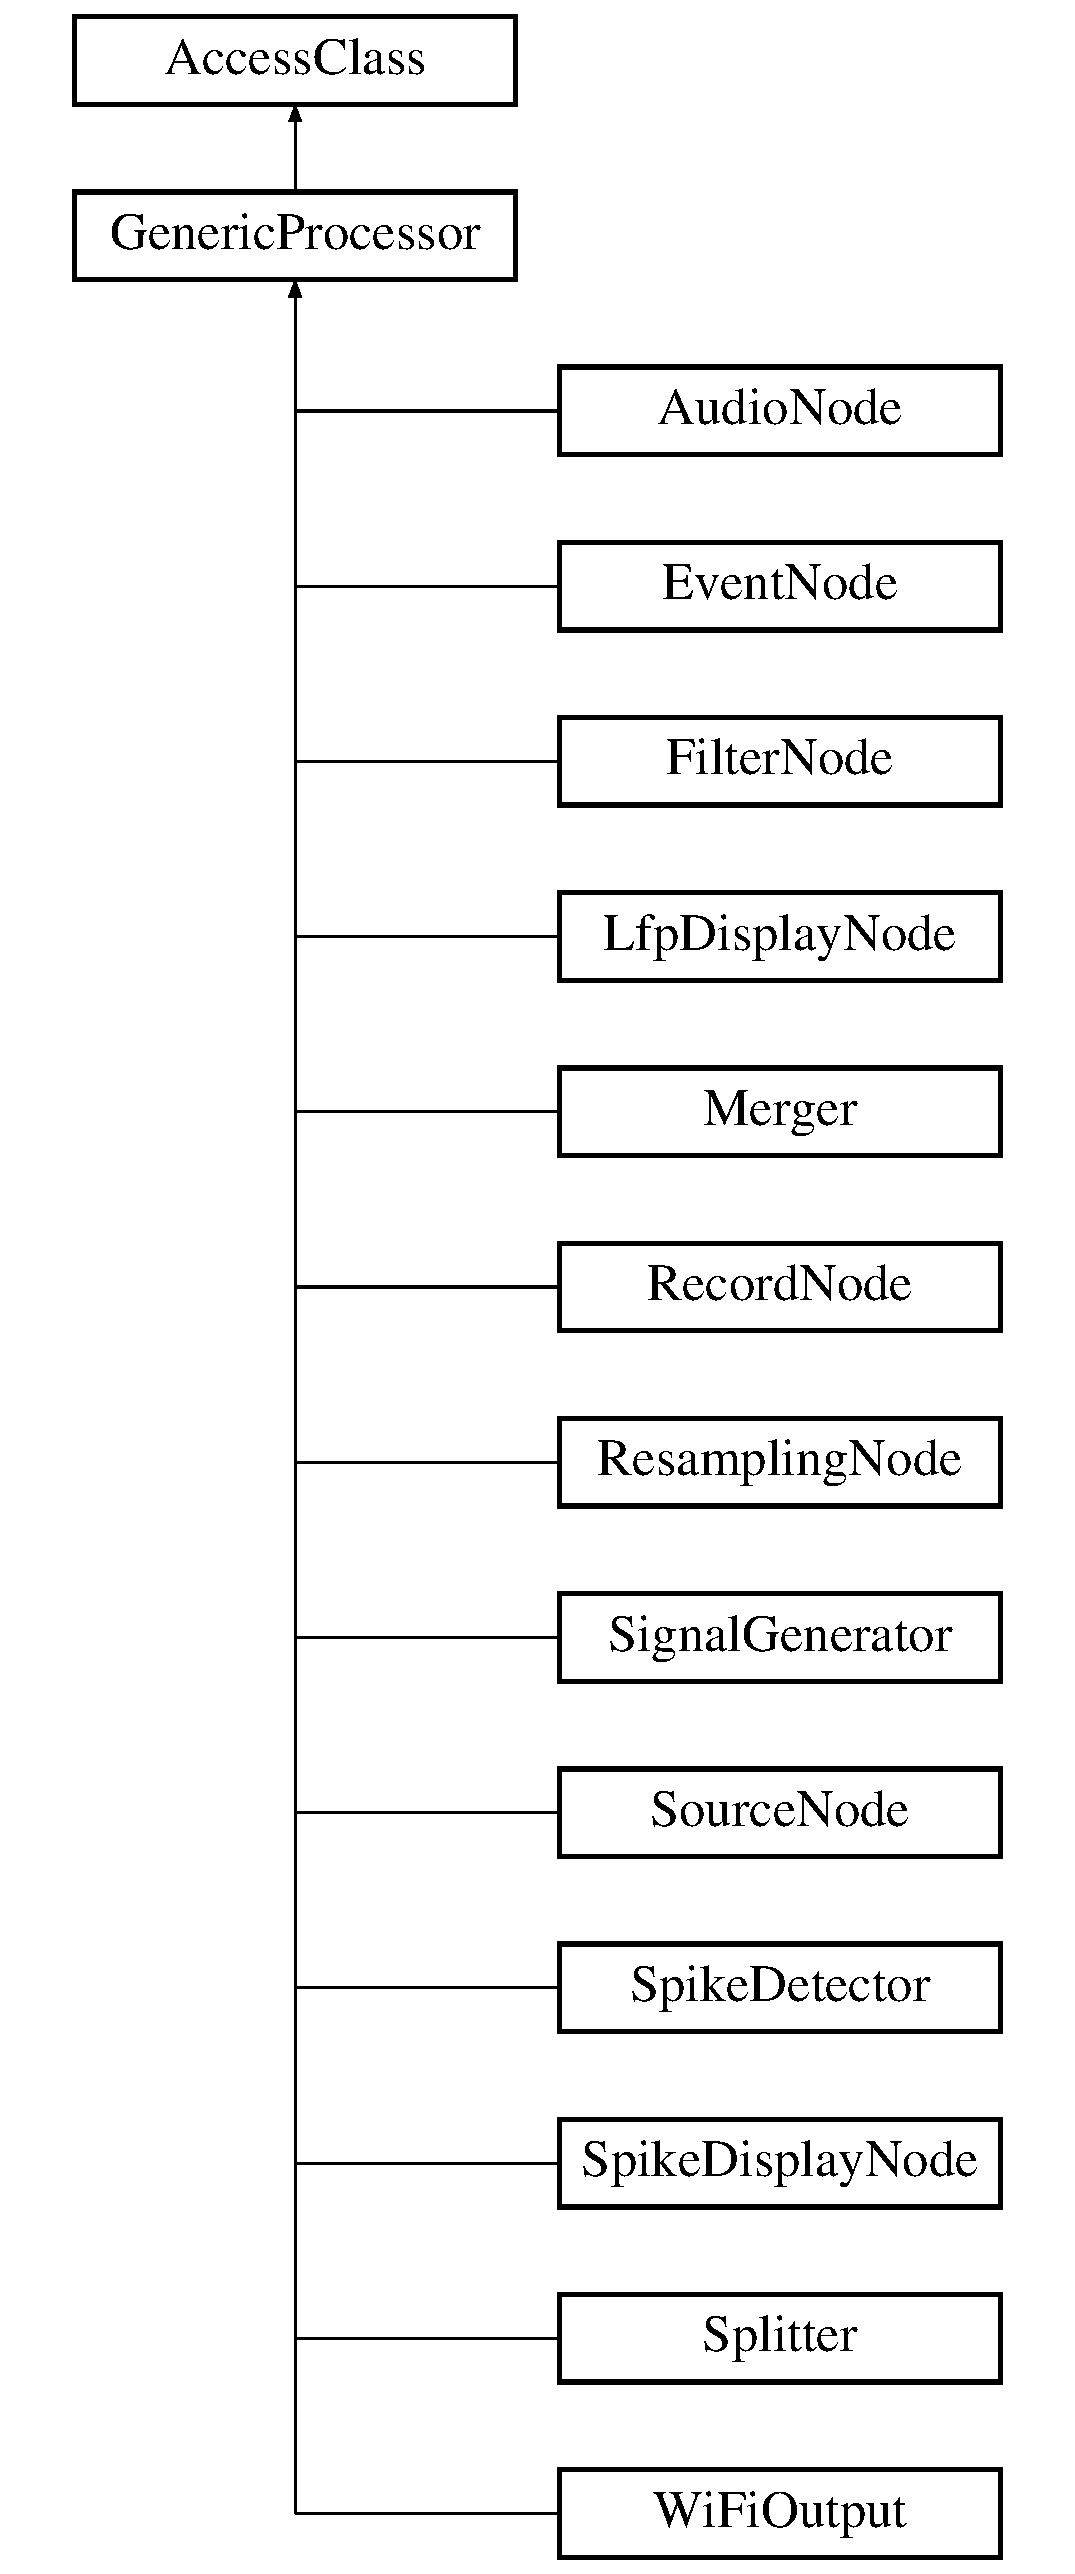
\includegraphics[height=12.000000cm]{classGenericProcessor}
\end{center}
\end{figure}
\subsection*{Classes}
\begin{DoxyCompactItemize}
\item 
struct \hyperlink{structGenericProcessor_1_1ProcessorSettings}{Processor\-Settings}
\end{DoxyCompactItemize}
\subsection*{Public Types}
\begin{DoxyCompactItemize}
\item 
enum {\bfseries event\-Types} \{ \\*
{\bfseries T\-I\-M\-E\-S\-T\-A\-M\-P} =  0, 
{\bfseries B\-U\-F\-F\-E\-R\-\_\-\-S\-I\-Z\-E} =  1, 
{\bfseries P\-A\-R\-A\-M\-E\-T\-E\-R\-\_\-\-C\-H\-A\-N\-G\-E} =  2, 
{\bfseries T\-T\-L} =  3, 
\\*
{\bfseries S\-P\-I\-K\-E} =  4, 
{\bfseries E\-E\-G} =  5, 
{\bfseries C\-O\-N\-T\-I\-N\-U\-O\-U\-S} =  6
 \}
\item 
enum {\bfseries event\-Channel\-Types} \{ {\bfseries G\-E\-N\-E\-R\-I\-C\-\_\-\-E\-V\-E\-N\-T} =  999, 
{\bfseries S\-I\-N\-G\-L\-E\-\_\-\-E\-L\-E\-C\-T\-R\-O\-D\-E} =  1, 
{\bfseries S\-T\-E\-R\-E\-O\-T\-R\-O\-D\-E} =  2, 
{\bfseries T\-E\-T\-R\-O\-D\-E} =  4
 \}
\end{DoxyCompactItemize}
\subsection*{Public Member Functions}
\begin{DoxyCompactItemize}
\item 
\hypertarget{classGenericProcessor_a907fc14eecca11021d9e129d0aee9700}{{\bfseries Generic\-Processor} (const String \&name\-\_\-)}\label{classGenericProcessor_a907fc14eecca11021d9e129d0aee9700}

\item 
\hypertarget{classGenericProcessor_aad3c1acb9fdeda122892ab9c5276119f}{const String {\bfseries get\-Name} () const }\label{classGenericProcessor_aad3c1acb9fdeda122892ab9c5276119f}

\item 
\hypertarget{classGenericProcessor_a38456d9796c0fcf521c173cf4338c728}{virtual void {\bfseries prepare\-To\-Play} (double sample\-Rate, int estimated\-Samples\-Per\-Block)}\label{classGenericProcessor_a38456d9796c0fcf521c173cf4338c728}

\item 
\hypertarget{classGenericProcessor_a53daa94f674d6b7e5e3d55fda717ec96}{void {\bfseries release\-Resources} ()}\label{classGenericProcessor_a53daa94f674d6b7e5e3d55fda717ec96}

\item 
\hypertarget{classGenericProcessor_ad8c8e91c2204a1d48d2d3b3bf117c09d}{virtual void {\bfseries set\-Parameter} (int parameter\-Index, float new\-Value)}\label{classGenericProcessor_ad8c8e91c2204a1d48d2d3b3bf117c09d}

\item 
\hypertarget{classGenericProcessor_a4336e8c17d1ba015933628d6902896fa}{virtual Audio\-Processor\-Editor $\ast$ {\bfseries create\-Editor} ()}\label{classGenericProcessor_a4336e8c17d1ba015933628d6902896fa}

\item 
\hypertarget{classGenericProcessor_a225a527d11f4ba694bc9557cf57ce656}{bool {\bfseries has\-Editor} () const }\label{classGenericProcessor_a225a527d11f4ba694bc9557cf57ce656}

\item 
\hypertarget{classGenericProcessor_ac5d607b4b7202294d26bbdbe61abd9a8}{void {\bfseries reset} ()}\label{classGenericProcessor_ac5d607b4b7202294d26bbdbe61abd9a8}

\item 
\hypertarget{classGenericProcessor_aab9014ebf17e362217a92f8f5b911e9d}{void {\bfseries set\-Current\-Program\-State\-Information} (const void $\ast$data, int size\-In\-Bytes)}\label{classGenericProcessor_aab9014ebf17e362217a92f8f5b911e9d}

\item 
\hypertarget{classGenericProcessor_ab405c546f5403871bf1855294a7cd0ff}{void {\bfseries set\-State\-Information} (const void $\ast$data, int size\-In\-Bytes)}\label{classGenericProcessor_ab405c546f5403871bf1855294a7cd0ff}

\item 
\hypertarget{classGenericProcessor_a472e86370ddb3adc0bb45aea1cca6dc0}{void {\bfseries get\-Current\-Program\-State\-Information} (Memory\-Block \&dest\-Data)}\label{classGenericProcessor_a472e86370ddb3adc0bb45aea1cca6dc0}

\item 
\hypertarget{classGenericProcessor_a042fc5bbfe1d25cc70b605fa7b591666}{void {\bfseries get\-State\-Information} (Memory\-Block \&dest\-Data)}\label{classGenericProcessor_a042fc5bbfe1d25cc70b605fa7b591666}

\item 
\hypertarget{classGenericProcessor_acf6b9ccfb9be861035dbb919d8fcc290}{void {\bfseries change\-Program\-Name} (int index, const String \&new\-Name)}\label{classGenericProcessor_acf6b9ccfb9be861035dbb919d8fcc290}

\item 
\hypertarget{classGenericProcessor_ac8949ad0240cb8f5167da076d1fc287b}{void {\bfseries set\-Current\-Program} (int index)}\label{classGenericProcessor_ac8949ad0240cb8f5167da076d1fc287b}

\item 
\hypertarget{classGenericProcessor_acc50df9e1f4d532070c4cf93f73c3766}{const String {\bfseries get\-Input\-Channel\-Name} (int channel\-Index) const }\label{classGenericProcessor_acc50df9e1f4d532070c4cf93f73c3766}

\item 
\hypertarget{classGenericProcessor_a58d462c3907932f6beed365b959b9e0e}{const String {\bfseries get\-Output\-Channel\-Name} (int channel\-Index) const }\label{classGenericProcessor_a58d462c3907932f6beed365b959b9e0e}

\item 
\hypertarget{classGenericProcessor_a353b144b431efafb2b830b1ff759c808}{const String {\bfseries get\-Parameter\-Name} (int parameter\-Index)}\label{classGenericProcessor_a353b144b431efafb2b830b1ff759c808}

\item 
\hypertarget{classGenericProcessor_abcfc1c5ffe90cb744e455d287e6059a6}{const String {\bfseries get\-Parameter\-Text} (int parameter\-Index)}\label{classGenericProcessor_abcfc1c5ffe90cb744e455d287e6059a6}

\item 
\hypertarget{classGenericProcessor_a58b6841219060ffda3a8ed8f34eea3ed}{const String {\bfseries get\-Program\-Name} (int index)}\label{classGenericProcessor_a58b6841219060ffda3a8ed8f34eea3ed}

\item 
\hypertarget{classGenericProcessor_a8809dc1000c5efec6b81d8080e586d5a}{bool {\bfseries is\-Input\-Channel\-Stereo\-Pair} (int index) const }\label{classGenericProcessor_a8809dc1000c5efec6b81d8080e586d5a}

\item 
\hypertarget{classGenericProcessor_a81b7c0491e5f7d9577b07db5652bed6c}{bool {\bfseries is\-Output\-Channel\-Stereo\-Pair} (int index) const }\label{classGenericProcessor_a81b7c0491e5f7d9577b07db5652bed6c}

\item 
\hypertarget{classGenericProcessor_af9133c109e5251413b322145aa7620b2}{bool {\bfseries accepts\-Midi} () const }\label{classGenericProcessor_af9133c109e5251413b322145aa7620b2}

\item 
\hypertarget{classGenericProcessor_af93f01089518726922286c9bb74419ee}{bool {\bfseries produces\-Midi} () const }\label{classGenericProcessor_af93f01089518726922286c9bb74419ee}

\item 
\hypertarget{classGenericProcessor_af7af56aa3afd875ed377d54f2ddeb941}{bool {\bfseries is\-Parameter\-Automatable} (int parameter\-Index)}\label{classGenericProcessor_af7af56aa3afd875ed377d54f2ddeb941}

\item 
\hypertarget{classGenericProcessor_a9a666aa80a84fdffcb2f3cf8b7599183}{bool {\bfseries is\-Meta\-Parameter} (int parameter\-Index)}\label{classGenericProcessor_a9a666aa80a84fdffcb2f3cf8b7599183}

\item 
\hypertarget{classGenericProcessor_a37f3bb2d2c4aa385b41f324beecc03eb}{int {\bfseries get\-Num\-Parameters} ()}\label{classGenericProcessor_a37f3bb2d2c4aa385b41f324beecc03eb}

\item 
\hypertarget{classGenericProcessor_ad80d3c00c3f8fa1a719196a447b9670d}{int {\bfseries get\-Num\-Programs} ()}\label{classGenericProcessor_ad80d3c00c3f8fa1a719196a447b9670d}

\item 
\hypertarget{classGenericProcessor_a13228cdfe7cd15d89bcc7c4061e0a797}{int {\bfseries get\-Current\-Program} ()}\label{classGenericProcessor_a13228cdfe7cd15d89bcc7c4061e0a797}

\item 
\hypertarget{classGenericProcessor_ae857c2fdef2d84ad20957a992889cdd7}{float {\bfseries get\-Parameter} (int parameter\-Index)}\label{classGenericProcessor_ae857c2fdef2d84ad20957a992889cdd7}

\item 
\hypertarget{classGenericProcessor_a7b3c8dcb0ba4bf1f71a65da4ad47f063}{\hyperlink{classParameter}{Parameter} \& {\bfseries get\-Parameter\-By\-Name} (String parameter\-Name)}\label{classGenericProcessor_a7b3c8dcb0ba4bf1f71a65da4ad47f063}

\item 
\hypertarget{classGenericProcessor_a1d58b5412eb6d031ad77ebf90cf7eeac}{\hyperlink{classParameter}{Parameter} \& {\bfseries get\-Parameter\-Reference} (int parameter\-Index)}\label{classGenericProcessor_a1d58b5412eb6d031ad77ebf90cf7eeac}

\item 
\hypertarget{classGenericProcessor_ac8746345d01c5de419d944ef20bc98e5}{virtual void {\bfseries process} (Audio\-Sample\-Buffer \&, Midi\-Buffer \&, int \&)=0}\label{classGenericProcessor_ac8746345d01c5de419d944ef20bc98e5}

\item 
\hypertarget{classGenericProcessor_a31f587ffcaddf91918013605d58651fe}{virtual float {\bfseries get\-Sample\-Rate} ()}\label{classGenericProcessor_a31f587ffcaddf91918013605d58651fe}

\item 
\hypertarget{classGenericProcessor_ad82b2eb662c16c4509ecd84d33e01eba}{virtual float {\bfseries get\-Default\-Sample\-Rate} ()}\label{classGenericProcessor_ad82b2eb662c16c4509ecd84d33e01eba}

\item 
\hypertarget{classGenericProcessor_aee3dea28d03bb09bdb4799343aaa2388}{virtual int {\bfseries get\-Num\-Inputs} ()}\label{classGenericProcessor_aee3dea28d03bb09bdb4799343aaa2388}

\item 
\hypertarget{classGenericProcessor_a25f5d4ef799bdb5029ea96eedf462bf3}{virtual int {\bfseries get\-Num\-Outputs} ()}\label{classGenericProcessor_a25f5d4ef799bdb5029ea96eedf462bf3}

\item 
\hypertarget{classGenericProcessor_aef569283cc91483814b210922cf96d26}{virtual int {\bfseries get\-Default\-Num\-Outputs} ()}\label{classGenericProcessor_aef569283cc91483814b210922cf96d26}

\item 
\hypertarget{classGenericProcessor_ac72dab4ba6fd23478986c4927d30ae46}{virtual float {\bfseries get\-Default\-Bit\-Volts} ()}\label{classGenericProcessor_ac72dab4ba6fd23478986c4927d30ae46}

\item 
\hypertarget{classGenericProcessor_a85a573cbf094b9e0b58caad89598b9b6}{virtual int {\bfseries get\-Next\-Channel} (bool)}\label{classGenericProcessor_a85a573cbf094b9e0b58caad89598b9b6}

\item 
\hypertarget{classGenericProcessor_a79f6e2e58b138bf070001d6bc8b7bb1d}{virtual void {\bfseries reset\-Connections} ()}\label{classGenericProcessor_a79f6e2e58b138bf070001d6bc8b7bb1d}

\item 
\hypertarget{classGenericProcessor_a887bc67d4ac284b65e3708e598845fa1}{virtual void {\bfseries set\-Current\-Channel} (int chan)}\label{classGenericProcessor_a887bc67d4ac284b65e3708e598845fa1}

\item 
\hypertarget{classGenericProcessor_ac9b78cf88078958fa27b08981f46e170}{int {\bfseries get\-Node\-Id} ()}\label{classGenericProcessor_ac9b78cf88078958fa27b08981f46e170}

\item 
\hypertarget{classGenericProcessor_a4d4245a009780a334517b0c242323f1b}{void {\bfseries set\-Node\-Id} (int id)}\label{classGenericProcessor_a4d4245a009780a334517b0c242323f1b}

\item 
\hypertarget{classGenericProcessor_a1f395b8e7bab82f54293337debcc9377}{\hyperlink{classGenericProcessor}{Generic\-Processor} $\ast$ {\bfseries get\-Source\-Node} ()}\label{classGenericProcessor_a1f395b8e7bab82f54293337debcc9377}

\item 
\hypertarget{classGenericProcessor_a222183cb80918b031531f381462a7a27}{\hyperlink{classGenericProcessor}{Generic\-Processor} $\ast$ {\bfseries get\-Dest\-Node} ()}\label{classGenericProcessor_a222183cb80918b031531f381462a7a27}

\item 
\hypertarget{classGenericProcessor_ab0fabe67cc2f3f8f5708ffba648a7178}{virtual void {\bfseries switch\-I\-O} (int)}\label{classGenericProcessor_ab0fabe67cc2f3f8f5708ffba648a7178}

\item 
\hypertarget{classGenericProcessor_a2081dd06eba70e46ba5770dbf04fadff}{virtual void {\bfseries switch\-I\-O} ()}\label{classGenericProcessor_a2081dd06eba70e46ba5770dbf04fadff}

\item 
\hypertarget{classGenericProcessor_a4aa819589398e892b3ceb89364db2b4c}{virtual void {\bfseries set\-Path\-To\-Processor} (\hyperlink{classGenericProcessor}{Generic\-Processor} $\ast$p)}\label{classGenericProcessor_a4aa819589398e892b3ceb89364db2b4c}

\item 
\hypertarget{classGenericProcessor_a6a21d25d3ad79fb4867c732c64322d54}{virtual void {\bfseries set\-Source\-Node} (\hyperlink{classGenericProcessor}{Generic\-Processor} $\ast$sn)}\label{classGenericProcessor_a6a21d25d3ad79fb4867c732c64322d54}

\item 
\hypertarget{classGenericProcessor_af133f0046c23153f46cc5aa3b6980b93}{virtual void {\bfseries set\-Dest\-Node} (\hyperlink{classGenericProcessor}{Generic\-Processor} $\ast$dn)}\label{classGenericProcessor_af133f0046c23153f46cc5aa3b6980b93}

\item 
\hypertarget{classGenericProcessor_aba1548d2f5671b90d9c9bf716fafaeb4}{virtual void {\bfseries set\-Merger\-Source\-Node} (\hyperlink{classGenericProcessor}{Generic\-Processor} $\ast$sn)}\label{classGenericProcessor_aba1548d2f5671b90d9c9bf716fafaeb4}

\item 
\hypertarget{classGenericProcessor_ac553d8495ef07f5971a1f2abd0506b7e}{virtual void {\bfseries set\-Splitter\-Dest\-Node} (\hyperlink{classGenericProcessor}{Generic\-Processor} $\ast$dn)}\label{classGenericProcessor_ac553d8495ef07f5971a1f2abd0506b7e}

\item 
\hypertarget{classGenericProcessor_ab24b6dcb56efe4b66ced5bdddf2093de}{virtual bool {\bfseries is\-Source} ()}\label{classGenericProcessor_ab24b6dcb56efe4b66ced5bdddf2093de}

\item 
\hypertarget{classGenericProcessor_a38f377ecefaad8269198403205159bb3}{virtual bool {\bfseries is\-Sink} ()}\label{classGenericProcessor_a38f377ecefaad8269198403205159bb3}

\item 
\hypertarget{classGenericProcessor_a990ea34d9f34d482ef26e618f7990b36}{virtual bool {\bfseries is\-Splitter} ()}\label{classGenericProcessor_a990ea34d9f34d482ef26e618f7990b36}

\item 
\hypertarget{classGenericProcessor_ab0a0cdb5233b92d5552e9db6566d1445}{virtual bool {\bfseries is\-Merger} ()}\label{classGenericProcessor_ab0a0cdb5233b92d5552e9db6566d1445}

\item 
\hypertarget{classGenericProcessor_a3802e6cb4f8bd84840408bae0434bb8e}{virtual bool {\bfseries can\-Send\-Signal\-To} (\hyperlink{classGenericProcessor}{Generic\-Processor} $\ast$)}\label{classGenericProcessor_a3802e6cb4f8bd84840408bae0434bb8e}

\item 
\hypertarget{classGenericProcessor_a019dc0a595127889b42e835b23db07f5}{virtual bool {\bfseries is\-Ready} ()}\label{classGenericProcessor_a019dc0a595127889b42e835b23db07f5}

\item 
\hypertarget{classGenericProcessor_aef8d92d5d667f0e9d4b2d334ddf37380}{virtual bool {\bfseries enable} ()}\label{classGenericProcessor_aef8d92d5d667f0e9d4b2d334ddf37380}

\item 
\hypertarget{classGenericProcessor_aac6a1a695bce499b07418efa1fde55f2}{virtual bool {\bfseries disable} ()}\label{classGenericProcessor_aac6a1a695bce499b07418efa1fde55f2}

\item 
\hypertarget{classGenericProcessor_a3f74e259858f741b6f1435ad8557884c}{virtual bool {\bfseries enabled\-State} ()}\label{classGenericProcessor_a3f74e259858f741b6f1435ad8557884c}

\item 
\hypertarget{classGenericProcessor_a82e6b660b3ccdd175b26ca1f7c89155e}{virtual void {\bfseries enabled\-State} (bool t)}\label{classGenericProcessor_a82e6b660b3ccdd175b26ca1f7c89155e}

\item 
\hypertarget{classGenericProcessor_ad5f545d93e0409b97f0f5a2a27a83b3a}{virtual void {\bfseries enable\-Current\-Channel} (bool)}\label{classGenericProcessor_ad5f545d93e0409b97f0f5a2a27a83b3a}

\item 
\hypertarget{classGenericProcessor_a93c1a537897142d16003a45661b95920}{virtual bool {\bfseries still\-Has\-Source} ()}\label{classGenericProcessor_a93c1a537897142d16003a45661b95920}

\item 
\hypertarget{classGenericProcessor_a2cc31f766d9e375cda9e240aa99d7f69}{virtual Audio\-Sample\-Buffer $\ast$ {\bfseries get\-Continuous\-Buffer} ()}\label{classGenericProcessor_a2cc31f766d9e375cda9e240aa99d7f69}

\item 
\hypertarget{classGenericProcessor_af0e8c9ba31626a779d4543b88925a0b1}{virtual Midi\-Buffer $\ast$ {\bfseries get\-Event\-Buffer} ()}\label{classGenericProcessor_af0e8c9ba31626a779d4543b88925a0b1}

\item 
\hypertarget{classGenericProcessor_a3670d2c14be198001b086cf9c8fc45b6}{virtual int {\bfseries check\-For\-Events} (Midi\-Buffer \&mb)}\label{classGenericProcessor_a3670d2c14be198001b086cf9c8fc45b6}

\item 
\hypertarget{classGenericProcessor_ad6edfd929eaffda941ebc61ebc8559a4}{virtual void {\bfseries add\-Event} (Midi\-Buffer \&mb, uint8 type, int sample\-Num, uint8 event\-I\-D=0, uint8 event\-Channel=0, uint8 num\-Bytes=0, uint8 $\ast$data=0)}\label{classGenericProcessor_ad6edfd929eaffda941ebc61ebc8559a4}

\item 
\hypertarget{classGenericProcessor_a304bd82f97d26b385dd99df04042723e}{virtual void {\bfseries handle\-Event} (int event\-Type, Midi\-Message \&event)}\label{classGenericProcessor_a304bd82f97d26b385dd99df04042723e}

\item 
\hypertarget{classGenericProcessor_ab2224d9c803f4282e8c8de729be58779}{virtual \hyperlink{classGenericEditor}{Generic\-Editor} $\ast$ {\bfseries get\-Editor} ()}\label{classGenericProcessor_ab2224d9c803f4282e8c8de729be58779}

\item 
\hypertarget{classGenericProcessor_a13960169926ae10febca934d12fbf4d7}{virtual bool {\bfseries is\-Audio\-Or\-Record\-Node} ()}\label{classGenericProcessor_a13960169926ae10febca934d12fbf4d7}

\item 
\hypertarget{classGenericProcessor_a6c4ac8dc9f66ffe8ccc100eb3cedbbe4}{virtual bool {\bfseries record\-Status} (int chan)}\label{classGenericProcessor_a6c4ac8dc9f66ffe8ccc100eb3cedbbe4}

\item 
\hypertarget{classGenericProcessor_a29cd0895c183a1edb44ab3b3e7f3b262}{virtual bool {\bfseries audio\-Status} (int chan)}\label{classGenericProcessor_a29cd0895c183a1edb44ab3b3e7f3b262}

\item 
\hypertarget{classGenericProcessor_a860285332129a657c4e479a1ba59fa18}{virtual void {\bfseries clear\-Settings} ()}\label{classGenericProcessor_a860285332129a657c4e479a1ba59fa18}

\item 
\hypertarget{classGenericProcessor_a5302ede3e22cc1511390dae4a7511766}{virtual void {\bfseries generate\-Default\-Channel\-Names} (String\-Array \&)}\label{classGenericProcessor_a5302ede3e22cc1511390dae4a7511766}

\item 
\hypertarget{classGenericProcessor_a73073787f0a760c1896522c934e94211}{virtual void {\bfseries update} ()}\label{classGenericProcessor_a73073787f0a760c1896522c934e94211}

\item 
\hypertarget{classGenericProcessor_a4020d7853cad011cbed7d71b5d6fddba}{virtual void {\bfseries update\-Settings} ()}\label{classGenericProcessor_a4020d7853cad011cbed7d71b5d6fddba}

\item 
\hypertarget{classGenericProcessor_a43c6c63d2650ca92a556b656e88544ac}{void {\bfseries set\-Start\-Channel} (int i)}\label{classGenericProcessor_a43c6c63d2650ca92a556b656e88544ac}

\item 
\hypertarget{classGenericProcessor_af4528a6eeda231a290eaa57676ebd6ec}{int {\bfseries get\-Start\-Channel} ()}\label{classGenericProcessor_af4528a6eeda231a290eaa57676ebd6ec}

\end{DoxyCompactItemize}
\subsection*{Public Attributes}
\begin{DoxyCompactItemize}
\item 
\hypertarget{classGenericProcessor_a0c25ce11948ca53f2028d05799b8396e}{\hyperlink{classGenericProcessor}{Generic\-Processor} $\ast$ {\bfseries source\-Node}}\label{classGenericProcessor_a0c25ce11948ca53f2028d05799b8396e}

\item 
\hypertarget{classGenericProcessor_a3ad44d191c2086d2cfbf2d6c0dbc8fc8}{\hyperlink{classGenericProcessor}{Generic\-Processor} $\ast$ {\bfseries dest\-Node}}\label{classGenericProcessor_a3ad44d191c2086d2cfbf2d6c0dbc8fc8}

\item 
\hypertarget{classGenericProcessor_a246d0fc22327b8488bbf8f59244c3254}{bool {\bfseries is\-Enabled}}\label{classGenericProcessor_a246d0fc22327b8488bbf8f59244c3254}

\item 
\hypertarget{classGenericProcessor_a49e52ec50d06b105a31a6c210e90ad64}{bool {\bfseries was\-Connected}}\label{classGenericProcessor_a49e52ec50d06b105a31a6c210e90ad64}

\item 
\hypertarget{classGenericProcessor_a1b3ee7e7633630f4bfb249e238b26f0f}{int {\bfseries next\-Available\-Channel}}\label{classGenericProcessor_a1b3ee7e7633630f4bfb249e238b26f0f}

\item 
\hypertarget{classGenericProcessor_adf4d162c8152a5396b44f3ed06ddd0d5}{int {\bfseries save\-Order}}\label{classGenericProcessor_adf4d162c8152a5396b44f3ed06ddd0d5}

\item 
\hypertarget{classGenericProcessor_a9fbf3349950427f863e7ada1c358a2f7}{int {\bfseries load\-Order}}\label{classGenericProcessor_a9fbf3349950427f863e7ada1c358a2f7}

\item 
\hypertarget{classGenericProcessor_ae0027dc36c2b2148f3f939d8193975c2}{int {\bfseries current\-Channel}}\label{classGenericProcessor_ae0027dc36c2b2148f3f939d8193975c2}

\item 
\hypertarget{classGenericProcessor_a9d482fa552a6a45d417012351bd2f6d3}{Scoped\-Pointer$<$ \hyperlink{classGenericEditor}{Generic\-Editor} $>$ {\bfseries editor}}\label{classGenericProcessor_a9d482fa552a6a45d417012351bd2f6d3}

\item 
\hypertarget{classGenericProcessor_afa3995f77ca03fa6b684869c58136dac}{\hyperlink{structGenericProcessor_1_1ProcessorSettings}{Processor\-Settings} {\bfseries settings}}\label{classGenericProcessor_afa3995f77ca03fa6b684869c58136dac}

\item 
\hypertarget{classGenericProcessor_a456658153f517e2e083134dcc4f6ec2a}{int {\bfseries node\-Id}}\label{classGenericProcessor_a456658153f517e2e083134dcc4f6ec2a}

\item 
\hypertarget{classGenericProcessor_a6cbe35e8fda628f79bdf246e37094af7}{Array$<$ \hyperlink{classParameter}{Parameter} $>$ {\bfseries parameters}}\label{classGenericProcessor_a6cbe35e8fda628f79bdf246e37094af7}

\item 
\hypertarget{classGenericProcessor_a7d2b1ae9789baa1804650c34ea555fb7}{String\-Array {\bfseries parameter\-Names}}\label{classGenericProcessor_a7d2b1ae9789baa1804650c34ea555fb7}

\item 
\hypertarget{classGenericProcessor_ab771cefa0d0e56f9d2d407cbd9f0b5bc}{\hyperlink{classParameter}{Parameter} {\bfseries null\-Param}}\label{classGenericProcessor_ab771cefa0d0e56f9d2d407cbd9f0b5bc}

\end{DoxyCompactItemize}
\subsection*{Private Member Functions}
\begin{DoxyCompactItemize}
\item 
\hypertarget{classGenericProcessor_ae7c809c188d64cc7a96c228cdb3d8e8f}{void {\bfseries process\-Block} (Audio\-Sample\-Buffer \&buffer, Midi\-Buffer \&midi\-Messages)}\label{classGenericProcessor_ae7c809c188d64cc7a96c228cdb3d8e8f}

\item 
\hypertarget{classGenericProcessor_a1406d9294c8cb4620b0bca29022a69ad}{int {\bfseries get\-Num\-Samples} (Midi\-Buffer \&)}\label{classGenericProcessor_a1406d9294c8cb4620b0bca29022a69ad}

\item 
\hypertarget{classGenericProcessor_afaeccbbd1bcd2b03b6645c48c6797124}{void {\bfseries set\-Num\-Samples} (Midi\-Buffer \&, int)}\label{classGenericProcessor_afaeccbbd1bcd2b03b6645c48c6797124}

\item 
\hypertarget{classGenericProcessor_a05bf8084cc6f77b3489757dcffb87c12}{{\bfseries J\-U\-C\-E\-\_\-\-D\-E\-C\-L\-A\-R\-E\-\_\-\-N\-O\-N\-\_\-\-C\-O\-P\-Y\-A\-B\-L\-E\-\_\-\-W\-I\-T\-H\-\_\-\-L\-E\-A\-K\-\_\-\-D\-E\-T\-E\-C\-T\-O\-R} (\hyperlink{classGenericProcessor}{Generic\-Processor})}\label{classGenericProcessor_a05bf8084cc6f77b3489757dcffb87c12}

\end{DoxyCompactItemize}
\subsection*{Private Attributes}
\begin{DoxyCompactItemize}
\item 
\hypertarget{classGenericProcessor_a940419f6cc9ce107f55d7b1a167341d1}{int {\bfseries audio\-And\-Record\-Node\-Start\-Channel}}\label{classGenericProcessor_a940419f6cc9ce107f55d7b1a167341d1}

\item 
\hypertarget{classGenericProcessor_a1491a414e1158d269bc3fd5fb58282e5}{const String {\bfseries name}}\label{classGenericProcessor_a1491a414e1158d269bc3fd5fb58282e5}

\end{DoxyCompactItemize}


The documentation for this class was generated from the following file\-:\begin{DoxyCompactItemize}
\item 
Processors/Generic\-Processor.\-h\end{DoxyCompactItemize}

\hypertarget{classImageIcon}{\section{Image\-Icon Class Reference}
\label{classImageIcon}\index{Image\-Icon@{Image\-Icon}}
}
\subsection*{Public Member Functions}
\begin{DoxyCompactItemize}
\item 
\hypertarget{classImageIcon_a02707e8134452585d3a0a915928547d1}{{\bfseries Image\-Icon} (Image \&image\-\_\-)}\label{classImageIcon_a02707e8134452585d3a0a915928547d1}

\item 
\hypertarget{classImageIcon_a6b38b917770b9c5c1b6469efd4c89138}{void {\bfseries set\-Opacity} (float)}\label{classImageIcon_a6b38b917770b9c5c1b6469efd4c89138}

\end{DoxyCompactItemize}
\subsection*{Private Member Functions}
\begin{DoxyCompactItemize}
\item 
\hypertarget{classImageIcon_ab12ecd9ab8c6f1a576b217df0ad64659}{void {\bfseries paint} (Graphics \&g)}\label{classImageIcon_ab12ecd9ab8c6f1a576b217df0ad64659}

\end{DoxyCompactItemize}
\subsection*{Private Attributes}
\begin{DoxyCompactItemize}
\item 
\hypertarget{classImageIcon_a09184ff95a20d7bb92654bf9ed3cc71e}{Image {\bfseries image}}\label{classImageIcon_a09184ff95a20d7bb92654bf9ed3cc71e}

\item 
\hypertarget{classImageIcon_aedd60183e8c61a72d7a350c506aea662}{float {\bfseries opacity}}\label{classImageIcon_aedd60183e8c61a72d7a350c506aea662}

\end{DoxyCompactItemize}


The documentation for this class was generated from the following file\-:\begin{DoxyCompactItemize}
\item 
Processors/\-Editors/Image\-Icon.\-h\end{DoxyCompactItemize}

\hypertarget{classInfoLabel}{\section{Info\-Label Class Reference}
\label{classInfoLabel}\index{Info\-Label@{Info\-Label}}
}


{\ttfamily \#include $<$Info\-Label.\-h$>$}

Inheritance diagram for Info\-Label\-:\begin{figure}[H]
\begin{center}
\leavevmode
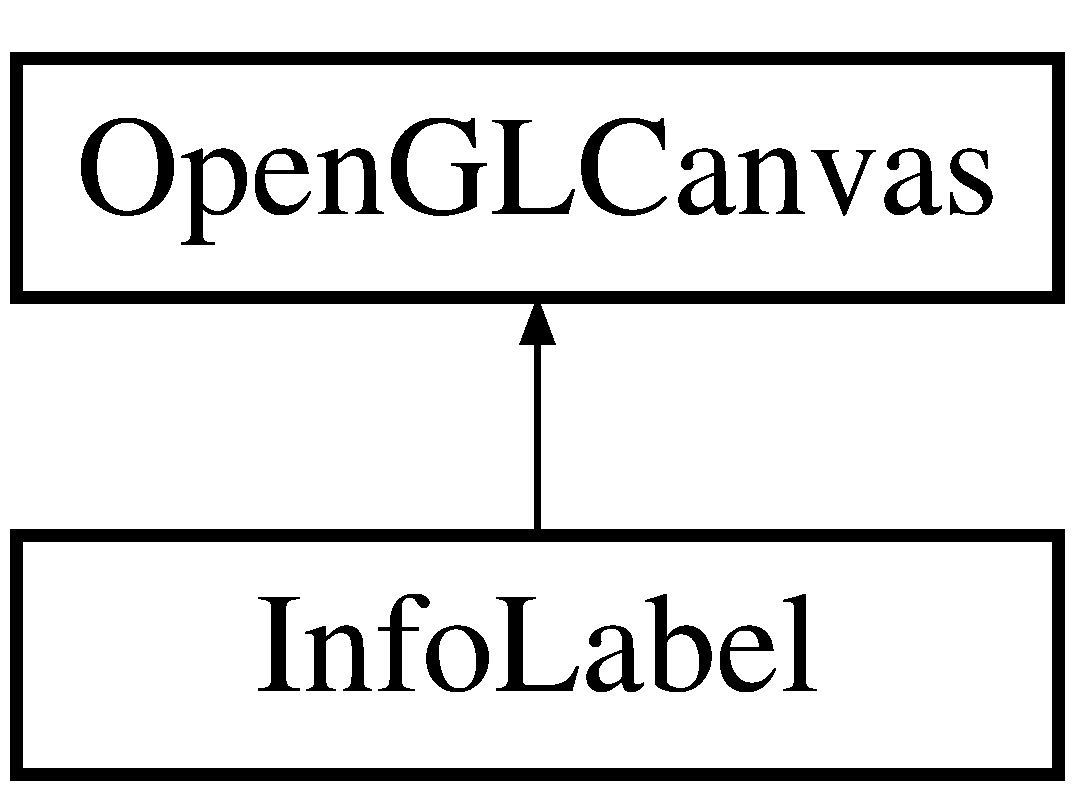
\includegraphics[height=2.000000cm]{classInfoLabel}
\end{center}
\end{figure}
\subsection*{Public Member Functions}
\begin{DoxyCompactItemize}
\item 
\hypertarget{classInfoLabel_ac7cfb1fffddb888a31e887b1ae9b89ae}{void {\bfseries new\-Open\-G\-L\-Context\-Created} ()}\label{classInfoLabel_ac7cfb1fffddb888a31e887b1ae9b89ae}

\item 
\hypertarget{classInfoLabel_a08e0dac049fd82431fbc6837f1d05347}{void {\bfseries render\-Open\-G\-L} ()}\label{classInfoLabel_a08e0dac049fd82431fbc6837f1d05347}

\end{DoxyCompactItemize}
\subsection*{Private Member Functions}
\begin{DoxyCompactItemize}
\item 
\hypertarget{classInfoLabel_a6f36d45e3b1ed07bd6e5ceb20cbcae4f}{void {\bfseries draw\-Label} ()}\label{classInfoLabel_a6f36d45e3b1ed07bd6e5ceb20cbcae4f}

\item 
\hypertarget{classInfoLabel_a6a9c140cdce03c12e09507cd6cefa628}{int {\bfseries get\-Total\-Height} ()}\label{classInfoLabel_a6a9c140cdce03c12e09507cd6cefa628}

\item 
\hypertarget{classInfoLabel_a80a01982ced2a1445e53937f8897b475}{void {\bfseries canvas\-Was\-Resized} ()}\label{classInfoLabel_a80a01982ced2a1445e53937f8897b475}

\item 
\hypertarget{classInfoLabel_ad72a0146997a1669d1af7231725629a3}{{\bfseries J\-U\-C\-E\-\_\-\-D\-E\-C\-L\-A\-R\-E\-\_\-\-N\-O\-N\-\_\-\-C\-O\-P\-Y\-A\-B\-L\-E\-\_\-\-W\-I\-T\-H\-\_\-\-L\-E\-A\-K\-\_\-\-D\-E\-T\-E\-C\-T\-O\-R} (\hyperlink{classInfoLabel}{Info\-Label})}\label{classInfoLabel_ad72a0146997a1669d1af7231725629a3}

\end{DoxyCompactItemize}
\subsection*{Private Attributes}
\begin{DoxyCompactItemize}
\item 
\hypertarget{classInfoLabel_a582db0e12e0a3a365b01163e58e0ba3f}{int {\bfseries x\-Buffer}}\label{classInfoLabel_a582db0e12e0a3a365b01163e58e0ba3f}

\item 
\hypertarget{classInfoLabel_a287a6f4f7b22b2c42d8cafef1531fb40}{int {\bfseries y\-Buffer}}\label{classInfoLabel_a287a6f4f7b22b2c42d8cafef1531fb40}

\item 
\hypertarget{classInfoLabel_ac413074578bd7931adf1ec946e6dc191}{F\-T\-Simple\-Layout {\bfseries layout}}\label{classInfoLabel_ac413074578bd7931adf1ec946e6dc191}

\item 
\hypertarget{classInfoLabel_a58b89957e778c566710f9d961f775b01}{String {\bfseries info\-String}}\label{classInfoLabel_a58b89957e778c566710f9d961f775b01}

\end{DoxyCompactItemize}
\subsection*{Additional Inherited Members}


\subsection{Detailed Description}
Displays general instructions about how to use the application.

Inhabits a tab in the \hyperlink{classDataViewport}{Data\-Viewport}.

\begin{DoxySeeAlso}{See also}
\hyperlink{classUIComponent}{U\-I\-Component}, \hyperlink{classDataViewport}{Data\-Viewport} 
\end{DoxySeeAlso}


The documentation for this class was generated from the following file\-:\begin{DoxyCompactItemize}
\item 
U\-I/Info\-Label.\-h\end{DoxyCompactItemize}

\hypertarget{classIntanThread}{\section{Intan\-Thread Class Reference}
\label{classIntanThread}\index{Intan\-Thread@{Intan\-Thread}}
}
Inheritance diagram for Intan\-Thread\-:\begin{figure}[H]
\begin{center}
\leavevmode
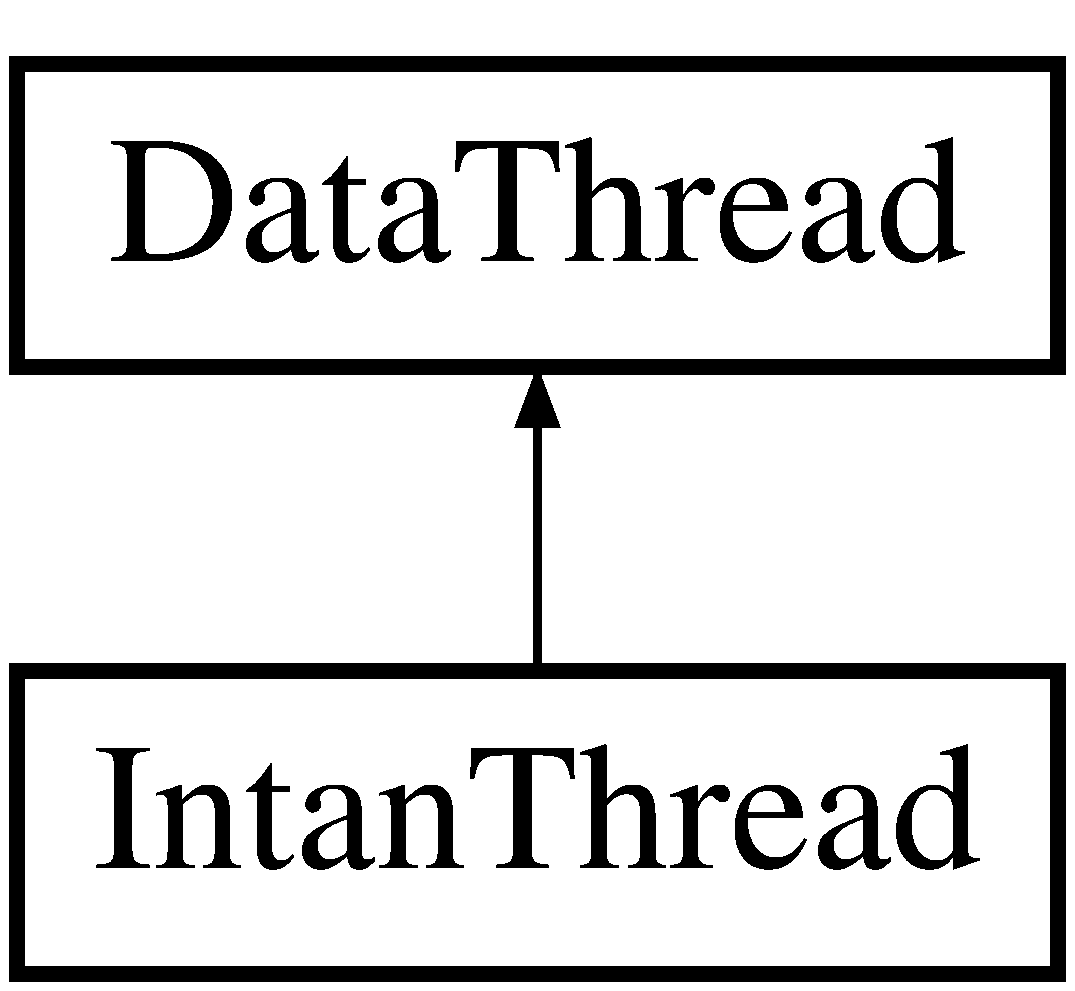
\includegraphics[height=2.000000cm]{classIntanThread}
\end{center}
\end{figure}
\subsection*{Public Member Functions}
\begin{DoxyCompactItemize}
\item 
\hypertarget{classIntanThread_ab42cbde857103d37c88bbf3d7df247eb}{{\bfseries Intan\-Thread} (\hyperlink{classSourceNode}{Source\-Node} $\ast$sn)}\label{classIntanThread_ab42cbde857103d37c88bbf3d7df247eb}

\item 
\hypertarget{classIntanThread_acd7222cc5aa5495fc9b99ccc89b57fc2}{bool {\bfseries found\-Input\-Source} ()}\label{classIntanThread_acd7222cc5aa5495fc9b99ccc89b57fc2}

\item 
\hypertarget{classIntanThread_a8b5d9057c93ce0e476e994274cdd35fc}{int {\bfseries get\-Num\-Channels} ()}\label{classIntanThread_a8b5d9057c93ce0e476e994274cdd35fc}

\item 
\hypertarget{classIntanThread_af75991b755889843df9e30e259fe7465}{float {\bfseries get\-Sample\-Rate} ()}\label{classIntanThread_af75991b755889843df9e30e259fe7465}

\item 
\hypertarget{classIntanThread_ad2020007cf90134f414a6c0413e63127}{float {\bfseries get\-Bit\-Volts} ()}\label{classIntanThread_ad2020007cf90134f414a6c0413e63127}

\end{DoxyCompactItemize}
\subsection*{Private Member Functions}
\begin{DoxyCompactItemize}
\item 
\hypertarget{classIntanThread_ad3ec9cdaf468082f5e5b58c8402c82f2}{bool {\bfseries initialize\-U\-S\-B} (bool)}\label{classIntanThread_ad3ec9cdaf468082f5e5b58c8402c82f2}

\item 
\hypertarget{classIntanThread_a2a9bb54b8e87969d8b946a6a20936392}{bool {\bfseries close\-U\-S\-B} ()}\label{classIntanThread_a2a9bb54b8e87969d8b946a6a20936392}

\item 
\hypertarget{classIntanThread_adbbfb2e7c3731875a9a2bcc8efdae038}{bool {\bfseries start\-Acquisition} ()}\label{classIntanThread_adbbfb2e7c3731875a9a2bcc8efdae038}

\item 
\hypertarget{classIntanThread_a2950c58ba91e3a4f717516cfa48733da}{bool {\bfseries stop\-Acquisition} ()}\label{classIntanThread_a2950c58ba91e3a4f717516cfa48733da}

\item 
\hypertarget{classIntanThread_a40a6417cb852d65de460f18370391c86}{bool {\bfseries update\-Buffer} ()}\label{classIntanThread_a40a6417cb852d65de460f18370391c86}

\item 
\hypertarget{classIntanThread_ad2c507a9a429e1e23bf43268a6c57545}{{\bfseries J\-U\-C\-E\-\_\-\-D\-E\-C\-L\-A\-R\-E\-\_\-\-N\-O\-N\-\_\-\-C\-O\-P\-Y\-A\-B\-L\-E\-\_\-\-W\-I\-T\-H\-\_\-\-L\-E\-A\-K\-\_\-\-D\-E\-T\-E\-C\-T\-O\-R} (\hyperlink{classIntanThread}{Intan\-Thread})}\label{classIntanThread_ad2c507a9a429e1e23bf43268a6c57545}

\end{DoxyCompactItemize}
\subsection*{Private Attributes}
\begin{DoxyCompactItemize}
\item 
\hypertarget{classIntanThread_a37dbef0918583861834fede108f3d753}{struct ftdi\-\_\-context {\bfseries ftdic}}\label{classIntanThread_a37dbef0918583861834fede108f3d753}

\item 
\hypertarget{classIntanThread_abbd43910e0876c010eed8c98ecfdc8cd}{int {\bfseries vendor\-I\-D}}\label{classIntanThread_abbd43910e0876c010eed8c98ecfdc8cd}

\item 
\hypertarget{classIntanThread_a45370212da99d373c584f3449d234782}{int {\bfseries product\-I\-D}}\label{classIntanThread_a45370212da99d373c584f3449d234782}

\item 
\hypertarget{classIntanThread_a65a860c5a971cd06d04d1a8c2ab79d3f}{int {\bfseries baudrate}}\label{classIntanThread_a65a860c5a971cd06d04d1a8c2ab79d3f}

\item 
\hypertarget{classIntanThread_a84c105d2757d8754c47d5dd93df74b5b}{bool {\bfseries is\-Transmitting}}\label{classIntanThread_a84c105d2757d8754c47d5dd93df74b5b}

\item 
\hypertarget{classIntanThread_a511e2ff1aa94f4cb9587bbcdcd55f2b3}{bool {\bfseries device\-Found}}\label{classIntanThread_a511e2ff1aa94f4cb9587bbcdcd55f2b3}

\item 
\hypertarget{classIntanThread_ad6fdd19d2044eb3161924a160663f19f}{unsigned char {\bfseries start\-Code}}\label{classIntanThread_ad6fdd19d2044eb3161924a160663f19f}

\item 
\hypertarget{classIntanThread_a33ff5cf792130bbc0e8aafbb5c251073}{unsigned char {\bfseries stop\-Code}}\label{classIntanThread_a33ff5cf792130bbc0e8aafbb5c251073}

\item 
\hypertarget{classIntanThread_ac76338b0917a125e3cf89fe92dade29b}{unsigned char {\bfseries buffer} \mbox{[}240\mbox{]}}\label{classIntanThread_ac76338b0917a125e3cf89fe92dade29b}

\item 
\hypertarget{classIntanThread_a6e8567c4b60bd8490faf9b8a78c5f4c2}{float {\bfseries this\-Sample} \mbox{[}16\mbox{]}}\label{classIntanThread_a6e8567c4b60bd8490faf9b8a78c5f4c2}

\item 
\hypertarget{classIntanThread_af1ce1bc20b17eadd1906d74066d42f0d}{int {\bfseries ch}}\label{classIntanThread_af1ce1bc20b17eadd1906d74066d42f0d}

\end{DoxyCompactItemize}
\subsection*{Additional Inherited Members}


The documentation for this class was generated from the following file\-:\begin{DoxyCompactItemize}
\item 
Processors/\-Data\-Threads/Intan\-Thread.\-h\end{DoxyCompactItemize}

\hypertarget{classLfpDisplayCanvas}{\section{Lfp\-Display\-Canvas Class Reference}
\label{classLfpDisplayCanvas}\index{Lfp\-Display\-Canvas@{Lfp\-Display\-Canvas}}
}
Inheritance diagram for Lfp\-Display\-Canvas\-:\begin{figure}[H]
\begin{center}
\leavevmode
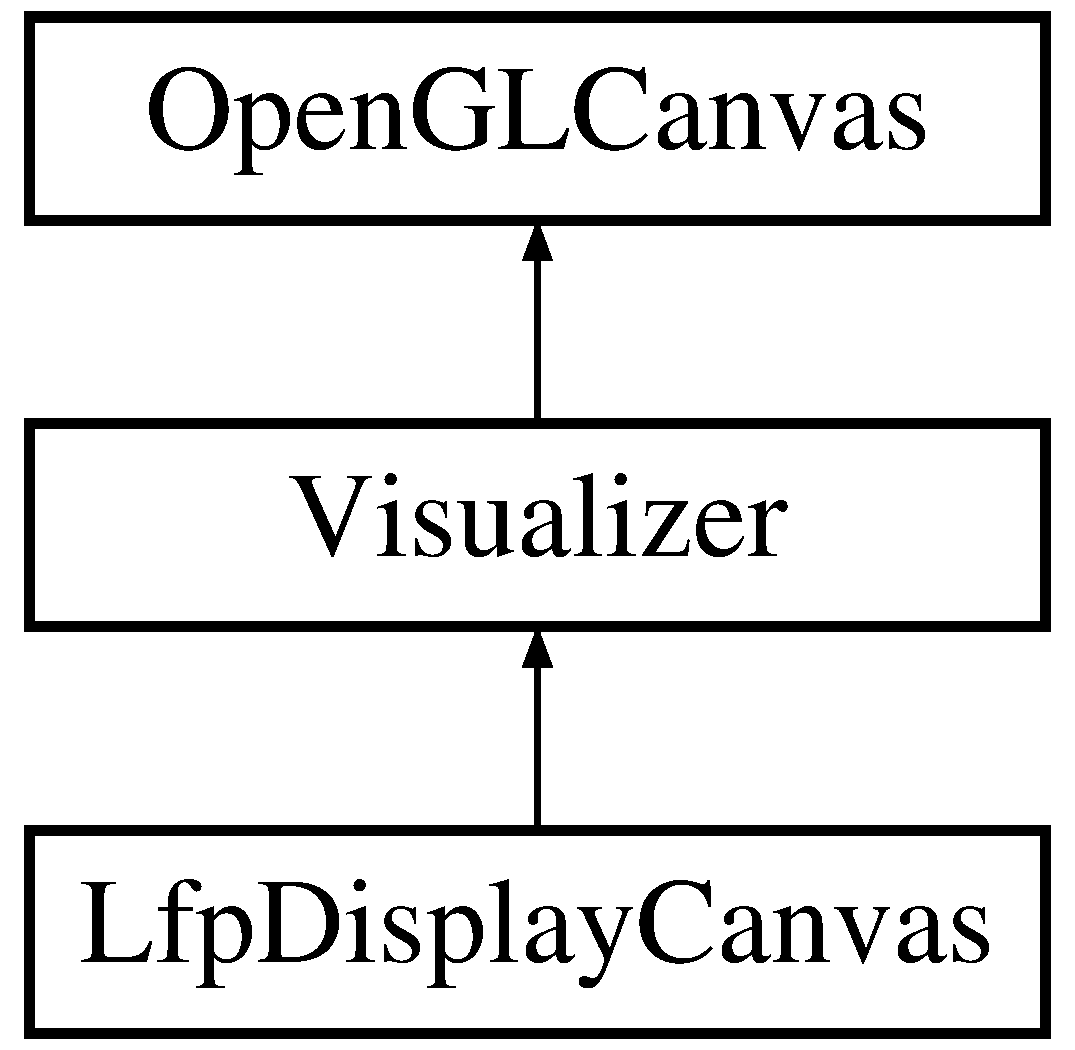
\includegraphics[height=3.000000cm]{classLfpDisplayCanvas}
\end{center}
\end{figure}
\subsection*{Public Member Functions}
\begin{DoxyCompactItemize}
\item 
\hypertarget{classLfpDisplayCanvas_adf1ecfecb9a4230a1b5ae4207c89dc40}{{\bfseries Lfp\-Display\-Canvas} (\hyperlink{classLfpDisplayNode}{Lfp\-Display\-Node} $\ast$n)}\label{classLfpDisplayCanvas_adf1ecfecb9a4230a1b5ae4207c89dc40}

\item 
\hypertarget{classLfpDisplayCanvas_a10420b4c6af6726fb855c05fb15ccdea}{void {\bfseries new\-Open\-G\-L\-Context\-Created} ()}\label{classLfpDisplayCanvas_a10420b4c6af6726fb855c05fb15ccdea}

\item 
\hypertarget{classLfpDisplayCanvas_ac952d1aedbf1097aec5619a0bbaf671d}{void {\bfseries render\-Open\-G\-L} ()}\label{classLfpDisplayCanvas_ac952d1aedbf1097aec5619a0bbaf671d}

\item 
\hypertarget{classLfpDisplayCanvas_aae6334f1eeac3da5167dce9ae72b53a2}{void {\bfseries begin\-Animation} ()}\label{classLfpDisplayCanvas_aae6334f1eeac3da5167dce9ae72b53a2}

\item 
\hypertarget{classLfpDisplayCanvas_af670120f5fdcee9c1c340f30b99fcf38}{void {\bfseries end\-Animation} ()}\label{classLfpDisplayCanvas_af670120f5fdcee9c1c340f30b99fcf38}

\item 
\hypertarget{classLfpDisplayCanvas_a14309c7e69190c5f6a983c497495555b}{void {\bfseries refresh\-State} ()}\label{classLfpDisplayCanvas_a14309c7e69190c5f6a983c497495555b}

\item 
\hypertarget{classLfpDisplayCanvas_a0f600e6a270078464154341dffd7312a}{void {\bfseries update} ()}\label{classLfpDisplayCanvas_a0f600e6a270078464154341dffd7312a}

\item 
\hypertarget{classLfpDisplayCanvas_a89a984c9c289a1a542474a5d3619e377}{void {\bfseries set\-Parameter} (int, float)}\label{classLfpDisplayCanvas_a89a984c9c289a1a542474a5d3619e377}

\item 
\hypertarget{classLfpDisplayCanvas_a8eea063f9627611e3aa5ff09518b8bfe}{void {\bfseries set\-Parameter} (int, int, int, float)}\label{classLfpDisplayCanvas_a8eea063f9627611e3aa5ff09518b8bfe}

\end{DoxyCompactItemize}
\subsection*{Private Member Functions}
\begin{DoxyCompactItemize}
\item 
\hypertarget{classLfpDisplayCanvas_a4ea0c0ccdfea78df6d005f846777d954}{void {\bfseries set\-Viewport} (int chan)}\label{classLfpDisplayCanvas_a4ea0c0ccdfea78df6d005f846777d954}

\item 
\hypertarget{classLfpDisplayCanvas_a3d72f13693b2d9ba8771b882f12934d2}{void {\bfseries draw\-Border} (bool is\-Selected)}\label{classLfpDisplayCanvas_a3d72f13693b2d9ba8771b882f12934d2}

\item 
\hypertarget{classLfpDisplayCanvas_ab24e9d1314dfa254b428b224caf4b6d8}{void {\bfseries draw\-Channel\-Info} (int chan, bool is\-Selected)}\label{classLfpDisplayCanvas_ab24e9d1314dfa254b428b224caf4b6d8}

\item 
\hypertarget{classLfpDisplayCanvas_af4c6a9771a6520959b21e7c4eccc59b0}{void {\bfseries draw\-Waveform} (int chan, bool is\-Selected)}\label{classLfpDisplayCanvas_af4c6a9771a6520959b21e7c4eccc59b0}

\item 
\hypertarget{classLfpDisplayCanvas_a741e76ee094b6d3c5745c5f787259779}{void {\bfseries draw\-Ticks} ()}\label{classLfpDisplayCanvas_a741e76ee094b6d3c5745c5f787259779}

\item 
\hypertarget{classLfpDisplayCanvas_aa26e3f1373b9f9c89a0180e2e37d59ac}{bool {\bfseries check\-Bounds} (int chan)}\label{classLfpDisplayCanvas_aa26e3f1373b9f9c89a0180e2e37d59ac}

\item 
\hypertarget{classLfpDisplayCanvas_acd9d9ff39590a4ee2be36655b194f99a}{void {\bfseries update\-Screen\-Buffer} ()}\label{classLfpDisplayCanvas_acd9d9ff39590a4ee2be36655b194f99a}

\item 
\hypertarget{classLfpDisplayCanvas_ac213eb3659a6e4dcd4adb78ca9a58d24}{int {\bfseries get\-Total\-Height} ()}\label{classLfpDisplayCanvas_ac213eb3659a6e4dcd4adb78ca9a58d24}

\item 
\hypertarget{classLfpDisplayCanvas_a0c38574ab7a847f8fd3aba7e00803772}{void {\bfseries canvas\-Was\-Resized} ()}\label{classLfpDisplayCanvas_a0c38574ab7a847f8fd3aba7e00803772}

\item 
\hypertarget{classLfpDisplayCanvas_ab3278e6eec42cdffaf5900e830872424}{void {\bfseries mouse\-Down\-In\-Canvas} (const Mouse\-Event \&e)}\label{classLfpDisplayCanvas_ab3278e6eec42cdffaf5900e830872424}

\item 
\hypertarget{classLfpDisplayCanvas_ac39b96bb7d4591a9215f9efa87394228}{{\bfseries J\-U\-C\-E\-\_\-\-D\-E\-C\-L\-A\-R\-E\-\_\-\-N\-O\-N\-\_\-\-C\-O\-P\-Y\-A\-B\-L\-E\-\_\-\-W\-I\-T\-H\-\_\-\-L\-E\-A\-K\-\_\-\-D\-E\-T\-E\-C\-T\-O\-R} (\hyperlink{classLfpDisplayCanvas}{Lfp\-Display\-Canvas})}\label{classLfpDisplayCanvas_ac39b96bb7d4591a9215f9efa87394228}

\end{DoxyCompactItemize}
\subsection*{Private Attributes}
\begin{DoxyCompactItemize}
\item 
\hypertarget{classLfpDisplayCanvas_a93b73f6af3deb7b991ed989fd31ecdb4}{int {\bfseries x\-Buffer}}\label{classLfpDisplayCanvas_a93b73f6af3deb7b991ed989fd31ecdb4}

\item 
\hypertarget{classLfpDisplayCanvas_a0ebed1e5d13dfbb27de142e7c52536b2}{int {\bfseries y\-Buffer}}\label{classLfpDisplayCanvas_a0ebed1e5d13dfbb27de142e7c52536b2}

\item 
\hypertarget{classLfpDisplayCanvas_a89e540f09a4f1ca02086f8a2577213e8}{float {\bfseries sample\-Rate}}\label{classLfpDisplayCanvas_a89e540f09a4f1ca02086f8a2577213e8}

\item 
\hypertarget{classLfpDisplayCanvas_a9e58888718eaf8b28afd3d09ef54d391}{float {\bfseries timebase}}\label{classLfpDisplayCanvas_a9e58888718eaf8b28afd3d09ef54d391}

\item 
\hypertarget{classLfpDisplayCanvas_a32be92992b63ec13baf20644bf049095}{float {\bfseries display\-Gain}}\label{classLfpDisplayCanvas_a32be92992b63ec13baf20644bf049095}

\item 
\hypertarget{classLfpDisplayCanvas_a15720a3c55775cdb623562a52db75ead}{\hyperlink{classLfpDisplayNode}{Lfp\-Display\-Node} $\ast$ {\bfseries processor}}\label{classLfpDisplayCanvas_a15720a3c55775cdb623562a52db75ead}

\item 
\hypertarget{classLfpDisplayCanvas_a8af8384c17db3f3f45ff5ae71ea03dec}{Audio\-Sample\-Buffer $\ast$ {\bfseries display\-Buffer}}\label{classLfpDisplayCanvas_a8af8384c17db3f3f45ff5ae71ea03dec}

\item 
\hypertarget{classLfpDisplayCanvas_a9f2c0112f64956caa7902d8522283a08}{Scoped\-Pointer$<$ Audio\-Sample\-Buffer $>$ {\bfseries screen\-Buffer}}\label{classLfpDisplayCanvas_a9f2c0112f64956caa7902d8522283a08}

\item 
\hypertarget{classLfpDisplayCanvas_ae933315568b66f703fcd736ba97d649a}{Midi\-Buffer $\ast$ {\bfseries event\-Buffer}}\label{classLfpDisplayCanvas_ae933315568b66f703fcd736ba97d649a}

\item 
\hypertarget{classLfpDisplayCanvas_ac97051e1ac0f4069e129044b58ce884c}{int {\bfseries screen\-Buffer\-Index}}\label{classLfpDisplayCanvas_ac97051e1ac0f4069e129044b58ce884c}

\item 
\hypertarget{classLfpDisplayCanvas_a8497c8b6130d06b0bd9ca18aa3872e5b}{int {\bfseries display\-Buffer\-Index}}\label{classLfpDisplayCanvas_a8497c8b6130d06b0bd9ca18aa3872e5b}

\item 
\hypertarget{classLfpDisplayCanvas_a480191897221f5a134fc7c83da2a3f74}{int {\bfseries display\-Buffer\-Size}}\label{classLfpDisplayCanvas_a480191897221f5a134fc7c83da2a3f74}

\item 
\hypertarget{classLfpDisplayCanvas_a05f5be2c61686fba7a1ad4291242d02e}{int {\bfseries n\-Chans}}\label{classLfpDisplayCanvas_a05f5be2c61686fba7a1ad4291242d02e}

\item 
\hypertarget{classLfpDisplayCanvas_a7c877cb51dfa4838aeef77431fff25e3}{int {\bfseries plot\-Height}}\label{classLfpDisplayCanvas_a7c877cb51dfa4838aeef77431fff25e3}

\item 
\hypertarget{classLfpDisplayCanvas_acd39c32e833762f1a75a3d5b0e85fb24}{int {\bfseries total\-Height}}\label{classLfpDisplayCanvas_acd39c32e833762f1a75a3d5b0e85fb24}

\item 
\hypertarget{classLfpDisplayCanvas_a618847c62242d50acf36e724270babab}{int {\bfseries selected\-Chan}}\label{classLfpDisplayCanvas_a618847c62242d50acf36e724270babab}

\end{DoxyCompactItemize}


The documentation for this class was generated from the following file\-:\begin{DoxyCompactItemize}
\item 
Processors/\-Visualization/Lfp\-Display\-Canvas.\-h\end{DoxyCompactItemize}

\hypertarget{classLfpDisplayEditor}{\section{Lfp\-Display\-Editor Class Reference}
\label{classLfpDisplayEditor}\index{Lfp\-Display\-Editor@{Lfp\-Display\-Editor}}
}
Inheritance diagram for Lfp\-Display\-Editor\-:\begin{figure}[H]
\begin{center}
\leavevmode
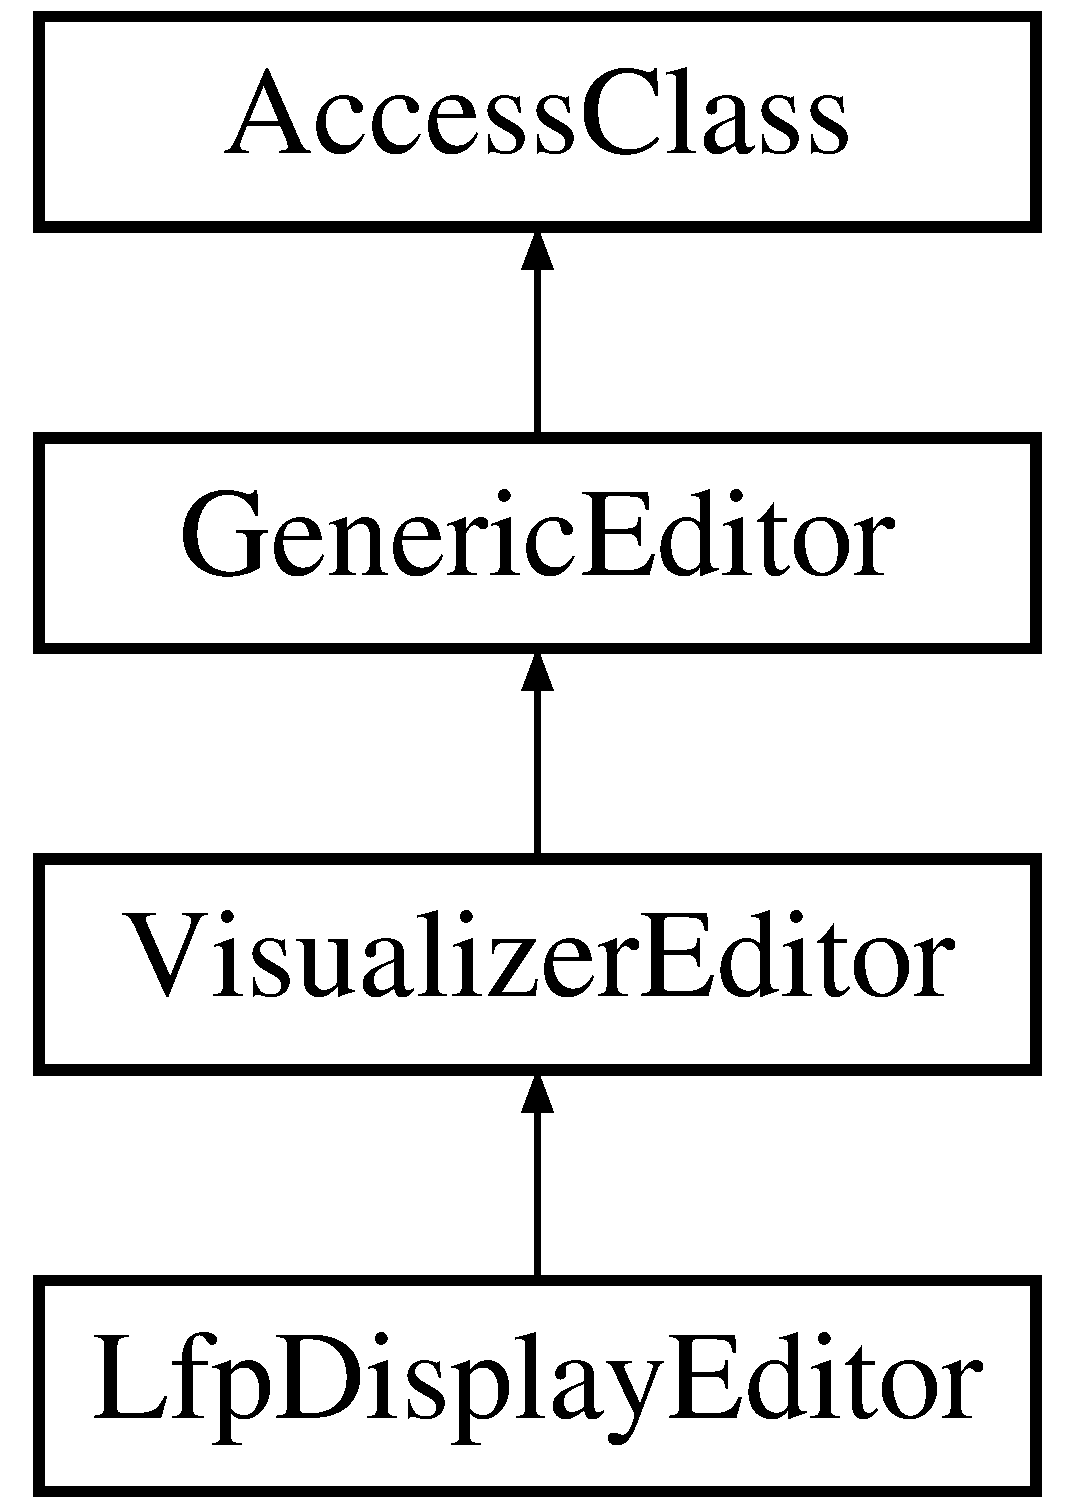
\includegraphics[height=4.000000cm]{classLfpDisplayEditor}
\end{center}
\end{figure}
\subsection*{Public Member Functions}
\begin{DoxyCompactItemize}
\item 
\hypertarget{classLfpDisplayEditor_a34f89fa14591e35a550261c57583f7fc}{{\bfseries Lfp\-Display\-Editor} (\hyperlink{classGenericProcessor}{Generic\-Processor} $\ast$)}\label{classLfpDisplayEditor_a34f89fa14591e35a550261c57583f7fc}

\item 
\hypertarget{classLfpDisplayEditor_a01b41c6ea44cafb27348520f14c1cf23}{void {\bfseries button\-Callback} (Button $\ast$button)}\label{classLfpDisplayEditor_a01b41c6ea44cafb27348520f14c1cf23}

\item 
\hypertarget{classLfpDisplayEditor_a86fa96fccccff6b684cb088cde7c08c0}{\hyperlink{classVisualizer}{Visualizer} $\ast$ {\bfseries create\-New\-Canvas} ()}\label{classLfpDisplayEditor_a86fa96fccccff6b684cb088cde7c08c0}

\end{DoxyCompactItemize}
\subsection*{Private Member Functions}
\begin{DoxyCompactItemize}
\item 
\hypertarget{classLfpDisplayEditor_af060c2d187023c967b9df63424b4b838}{{\bfseries J\-U\-C\-E\-\_\-\-D\-E\-C\-L\-A\-R\-E\-\_\-\-N\-O\-N\-\_\-\-C\-O\-P\-Y\-A\-B\-L\-E\-\_\-\-W\-I\-T\-H\-\_\-\-L\-E\-A\-K\-\_\-\-D\-E\-T\-E\-C\-T\-O\-R} (\hyperlink{classLfpDisplayEditor}{Lfp\-Display\-Editor})}\label{classLfpDisplayEditor_af060c2d187023c967b9df63424b4b838}

\end{DoxyCompactItemize}
\subsection*{Additional Inherited Members}


The documentation for this class was generated from the following file\-:\begin{DoxyCompactItemize}
\item 
Processors/\-Editors/Lfp\-Display\-Editor.\-h\end{DoxyCompactItemize}

\hypertarget{classLfpDisplayNode}{\section{Lfp\-Display\-Node Class Reference}
\label{classLfpDisplayNode}\index{Lfp\-Display\-Node@{Lfp\-Display\-Node}}
}
Inheritance diagram for Lfp\-Display\-Node\-:\begin{figure}[H]
\begin{center}
\leavevmode
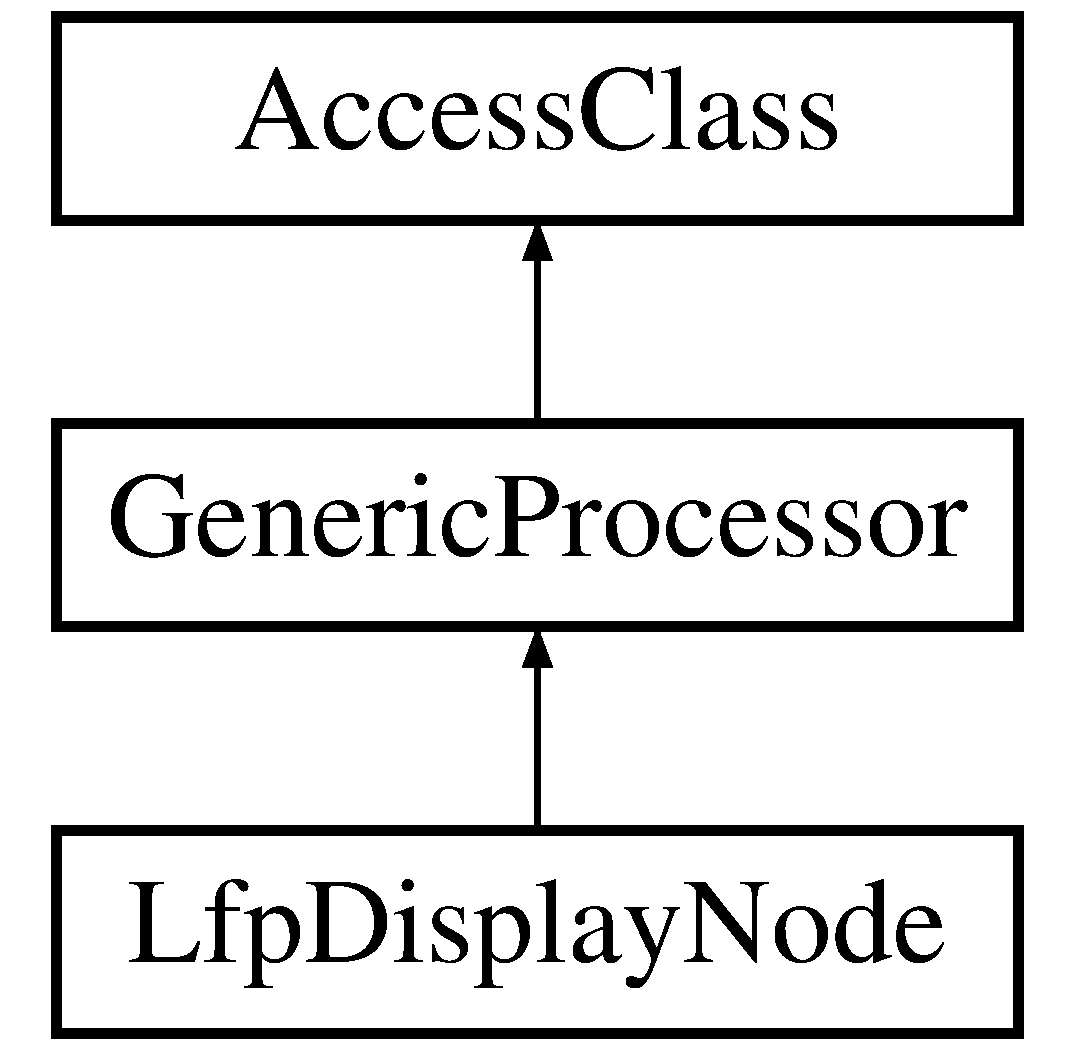
\includegraphics[height=3.000000cm]{classLfpDisplayNode}
\end{center}
\end{figure}
\subsection*{Public Member Functions}
\begin{DoxyCompactItemize}
\item 
\hypertarget{classLfpDisplayNode_ac5f35b216ebabf0ceb16c83d799d21d6}{Audio\-Processor\-Editor $\ast$ {\bfseries create\-Editor} ()}\label{classLfpDisplayNode_ac5f35b216ebabf0ceb16c83d799d21d6}

\item 
\hypertarget{classLfpDisplayNode_a313f1eee04b338d4c73414bf898710ca}{bool {\bfseries is\-Sink} ()}\label{classLfpDisplayNode_a313f1eee04b338d4c73414bf898710ca}

\item 
\hypertarget{classLfpDisplayNode_ae2060971a75911cf7fc91f4729eddc00}{void {\bfseries process} (Audio\-Sample\-Buffer \&buffer, Midi\-Buffer \&midi\-Messages, int \&n\-Samples)}\label{classLfpDisplayNode_ae2060971a75911cf7fc91f4729eddc00}

\item 
\hypertarget{classLfpDisplayNode_a1646cac1cf79906c032123ef5145337a}{void {\bfseries set\-Parameter} (int, float)}\label{classLfpDisplayNode_a1646cac1cf79906c032123ef5145337a}

\item 
\hypertarget{classLfpDisplayNode_ad83ef4ae6e745f6d92b56306850c9033}{void {\bfseries update\-Settings} ()}\label{classLfpDisplayNode_ad83ef4ae6e745f6d92b56306850c9033}

\item 
\hypertarget{classLfpDisplayNode_a6eb5f8069d42b172bd02ae4a49e7e272}{bool {\bfseries enable} ()}\label{classLfpDisplayNode_a6eb5f8069d42b172bd02ae4a49e7e272}

\item 
\hypertarget{classLfpDisplayNode_a002144f0fd7488eb47b519842a7ad738}{bool {\bfseries disable} ()}\label{classLfpDisplayNode_a002144f0fd7488eb47b519842a7ad738}

\item 
\hypertarget{classLfpDisplayNode_ab426013a5ed9be3bda32a732348c7c56}{Audio\-Sample\-Buffer $\ast$ {\bfseries get\-Display\-Buffer\-Address} ()}\label{classLfpDisplayNode_ab426013a5ed9be3bda32a732348c7c56}

\item 
\hypertarget{classLfpDisplayNode_a68f45d41fb62d834f91e170e471d3172}{int {\bfseries get\-Display\-Buffer\-Index} ()}\label{classLfpDisplayNode_a68f45d41fb62d834f91e170e471d3172}

\end{DoxyCompactItemize}
\subsection*{Private Member Functions}
\begin{DoxyCompactItemize}
\item 
\hypertarget{classLfpDisplayNode_a8e1bb9a83eb0c317c966fd29442f802d}{bool {\bfseries resize\-Buffer} ()}\label{classLfpDisplayNode_a8e1bb9a83eb0c317c966fd29442f802d}

\item 
\hypertarget{classLfpDisplayNode_a6f2053d848c703e0233ec71ffecf7647}{{\bfseries J\-U\-C\-E\-\_\-\-D\-E\-C\-L\-A\-R\-E\-\_\-\-N\-O\-N\-\_\-\-C\-O\-P\-Y\-A\-B\-L\-E\-\_\-\-W\-I\-T\-H\-\_\-\-L\-E\-A\-K\-\_\-\-D\-E\-T\-E\-C\-T\-O\-R} (\hyperlink{classLfpDisplayNode}{Lfp\-Display\-Node})}\label{classLfpDisplayNode_a6f2053d848c703e0233ec71ffecf7647}

\end{DoxyCompactItemize}
\subsection*{Private Attributes}
\begin{DoxyCompactItemize}
\item 
\hypertarget{classLfpDisplayNode_afa2c71f44d39677380462cef2c250a97}{Scoped\-Pointer$<$ Audio\-Sample\-Buffer $>$ {\bfseries display\-Buffer}}\label{classLfpDisplayNode_afa2c71f44d39677380462cef2c250a97}

\item 
\hypertarget{classLfpDisplayNode_adc4fbb762ccc4e7397355ec9611ea0a2}{Scoped\-Pointer$<$ Midi\-Buffer $>$ {\bfseries event\-Buffer}}\label{classLfpDisplayNode_adc4fbb762ccc4e7397355ec9611ea0a2}

\item 
\hypertarget{classLfpDisplayNode_a45b64282f7705772e1aa4221a8bf2740}{int {\bfseries display\-Buffer\-Index}}\label{classLfpDisplayNode_a45b64282f7705772e1aa4221a8bf2740}

\item 
\hypertarget{classLfpDisplayNode_a0d9b987e3f0010a7d75637048d507cc1}{float {\bfseries display\-Gain}}\label{classLfpDisplayNode_a0d9b987e3f0010a7d75637048d507cc1}

\item 
\hypertarget{classLfpDisplayNode_ae9bf0f1ff25193a4ca3cedd24006e652}{float {\bfseries buffer\-Length}}\label{classLfpDisplayNode_ae9bf0f1ff25193a4ca3cedd24006e652}

\item 
\hypertarget{classLfpDisplayNode_ab1ec98d120e9c66ecb4dbcfe2404966d}{Abstract\-Fifo {\bfseries abstract\-Fifo}}\label{classLfpDisplayNode_ab1ec98d120e9c66ecb4dbcfe2404966d}

\end{DoxyCompactItemize}
\subsection*{Additional Inherited Members}


The documentation for this class was generated from the following file\-:\begin{DoxyCompactItemize}
\item 
Processors/Lfp\-Display\-Node.\-h\end{DoxyCompactItemize}

\hypertarget{classLfpViewer}{\section{Lfp\-Viewer Class Reference}
\label{classLfpViewer}\index{Lfp\-Viewer@{Lfp\-Viewer}}
}


{\ttfamily \#include $<$Lfp\-Viewer.\-h$>$}

\subsection*{Public Member Functions}
\begin{DoxyCompactItemize}
\item 
\hypertarget{classLfpViewer_a899a37851745963d4ee126916ec3fa92}{{\bfseries Lfp\-Viewer} (Audio\-Sample\-Buffer $\ast$stream\-Buffer, Midi\-Buffer $\ast$event\-Buffer, \hyperlink{classUIComponent}{U\-I\-Component} $\ast$ui)}\label{classLfpViewer_a899a37851745963d4ee126916ec3fa92}

\item 
\hypertarget{classLfpViewer_a13eebe7f519efd288b89e1842cad0dcb}{void {\bfseries render\-Open\-G\-L} ()}\label{classLfpViewer_a13eebe7f519efd288b89e1842cad0dcb}

\item 
\hypertarget{classLfpViewer_a800d1460152411ae80c65041583c8cf0}{void {\bfseries new\-Open\-G\-L\-Context\-Created} ()}\label{classLfpViewer_a800d1460152411ae80c65041583c8cf0}

\item 
\hypertarget{classLfpViewer_aefb6893bd17adea3d652dabe9b8b554e}{void {\bfseries mouse\-Down} (const Mouse\-Event \&e)}\label{classLfpViewer_aefb6893bd17adea3d652dabe9b8b554e}

\end{DoxyCompactItemize}


\subsection{Detailed Description}
--T\-H\-I\-S F\-I\-L\-E I\-S O\-B\-S\-O\-L\-E\-T\-E, B\-U\-T R\-E\-M\-A\-I\-N\-S F\-O\-R R\-E\-F\-E\-R\-E\-N\-C\-E P\-U\-R\-P\-O\-S\-E\-S-- 

The documentation for this class was generated from the following file\-:\begin{DoxyCompactItemize}
\item 
Processors/\-Visualization/Lfp\-Viewer.\-h\end{DoxyCompactItemize}

\hypertarget{classMainWindow}{\section{Main\-Window Class Reference}
\label{classMainWindow}\index{Main\-Window@{Main\-Window}}
}


{\ttfamily \#include $<$Main\-Window.\-h$>$}

\subsection*{Public Member Functions}
\begin{DoxyCompactItemize}
\item 
\hypertarget{classMainWindow_ac422fd3f1931a97b30d5efc8b6fc3123}{void {\bfseries close\-Button\-Pressed} ()}\label{classMainWindow_ac422fd3f1931a97b30d5efc8b6fc3123}

\end{DoxyCompactItemize}
\subsection*{Public Attributes}
\begin{DoxyCompactItemize}
\item 
\hypertarget{classMainWindow_ae36bb0085b5650e00bca6bab107dc691}{Application\-Command\-Manager {\bfseries command\-Manager}}\label{classMainWindow_ae36bb0085b5650e00bca6bab107dc691}

\end{DoxyCompactItemize}
\subsection*{Private Member Functions}
\begin{DoxyCompactItemize}
\item 
\hypertarget{classMainWindow_ae568da7ab0da00891e838c197e9b0904}{void {\bfseries save\-Window\-Bounds} ()}\label{classMainWindow_ae568da7ab0da00891e838c197e9b0904}

\item 
\hypertarget{classMainWindow_a0787392bb77872c6765a390918cca794}{void {\bfseries load\-Window\-Bounds} ()}\label{classMainWindow_a0787392bb77872c6765a390918cca794}

\end{DoxyCompactItemize}
\subsection*{Private Attributes}
\begin{DoxyCompactItemize}
\item 
\hypertarget{classMainWindow_acdaba8b56c01e387346f503c46070d60}{\hyperlink{classAudioComponent}{Audio\-Component} $\ast$ {\bfseries audio\-Component}}\label{classMainWindow_acdaba8b56c01e387346f503c46070d60}

\item 
\hypertarget{classMainWindow_a5a30971233877ddb0bf2fb3436d39bfb}{\hyperlink{classProcessorGraph}{Processor\-Graph} $\ast$ {\bfseries processor\-Graph}}\label{classMainWindow_a5a30971233877ddb0bf2fb3436d39bfb}

\end{DoxyCompactItemize}


\subsection{Detailed Description}
The main window for the G\-U\-I application.

This object creates and destroys the \hyperlink{classAudioComponent}{Audio\-Component}, the \hyperlink{classProcessorGraph}{Processor\-Graph}, and the \hyperlink{classUIComponent}{U\-I\-Component} (which exists as the Content\-Component of this window).

\begin{DoxySeeAlso}{See also}
\hyperlink{classAudioComponent}{Audio\-Component}, \hyperlink{classProcessorGraph}{Processor\-Graph}, \hyperlink{classUIComponent}{U\-I\-Component} 
\end{DoxySeeAlso}


The documentation for this class was generated from the following file\-:\begin{DoxyCompactItemize}
\item 
Main\-Window.\-h\end{DoxyCompactItemize}

\hypertarget{classMerger}{\section{Merger Class Reference}
\label{classMerger}\index{Merger@{Merger}}
}


{\ttfamily \#include $<$Merger.\-h$>$}

Inheritance diagram for Merger\-:\begin{figure}[H]
\begin{center}
\leavevmode
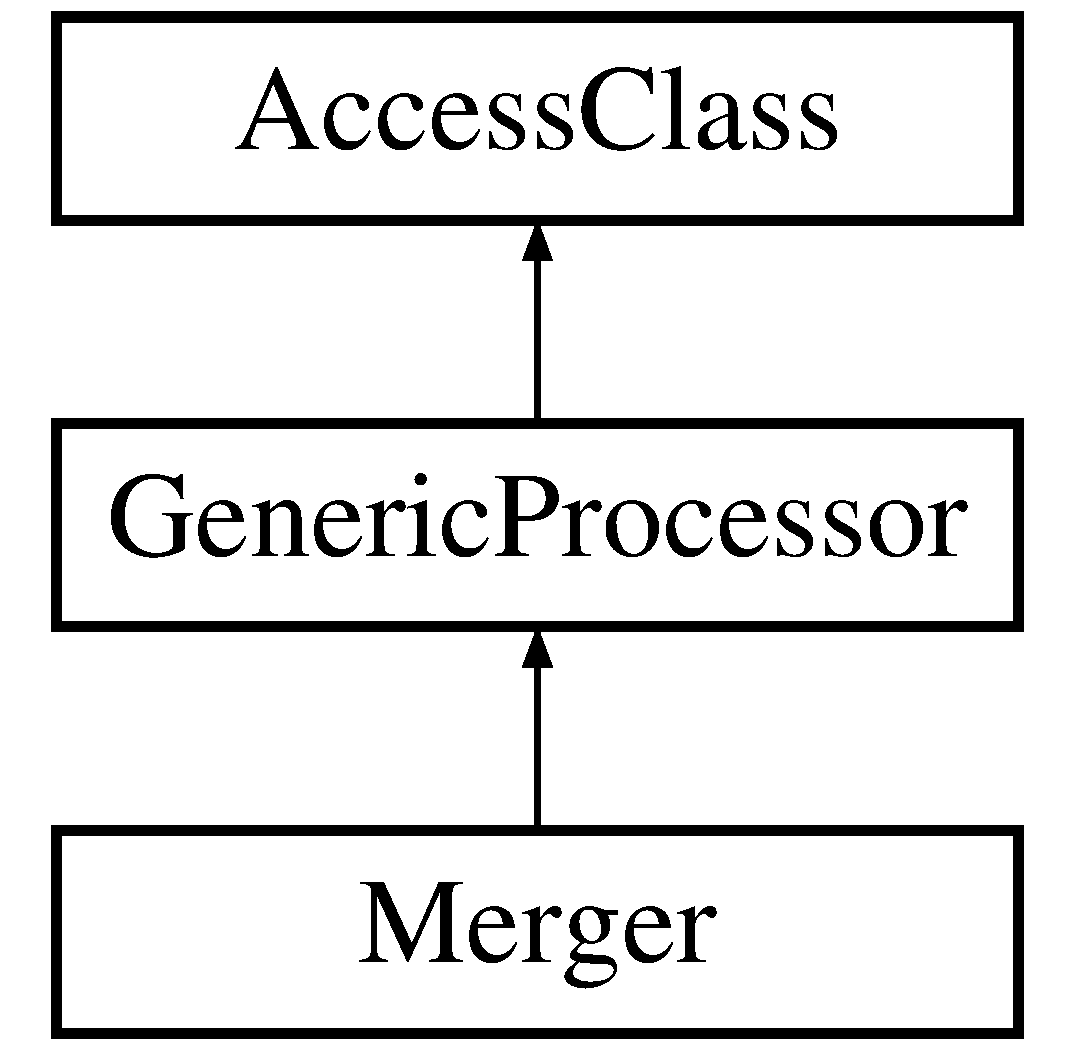
\includegraphics[height=3.000000cm]{classMerger}
\end{center}
\end{figure}
\subsection*{Public Member Functions}
\begin{DoxyCompactItemize}
\item 
\hypertarget{classMerger_a2e381efbef8d22df3b6522bb04325ced}{Audio\-Processor\-Editor $\ast$ {\bfseries create\-Editor} ()}\label{classMerger_a2e381efbef8d22df3b6522bb04325ced}

\item 
\hypertarget{classMerger_aa486022781477e2602efa1edac73d69a}{void {\bfseries process} (Audio\-Sample\-Buffer \&buffer, Midi\-Buffer \&midi\-Messages, int \&n\-Samples)}\label{classMerger_aa486022781477e2602efa1edac73d69a}

\item 
\hypertarget{classMerger_aff9f501ad9eb8bf1cd85570860cbc24c}{bool {\bfseries is\-Merger} ()}\label{classMerger_aff9f501ad9eb8bf1cd85570860cbc24c}

\item 
\hypertarget{classMerger_a7175efb6c9552ca22f9f902417232f06}{void {\bfseries switch\-I\-O} (int)}\label{classMerger_a7175efb6c9552ca22f9f902417232f06}

\item 
\hypertarget{classMerger_a23a05860a3235e426fbd4af0c149ea58}{void {\bfseries switch\-I\-O} ()}\label{classMerger_a23a05860a3235e426fbd4af0c149ea58}

\item 
\hypertarget{classMerger_a2017343133663806fea51c9a03688628}{void {\bfseries set\-Merger\-Source\-Node} (\hyperlink{classGenericProcessor}{Generic\-Processor} $\ast$sn)}\label{classMerger_a2017343133663806fea51c9a03688628}

\item 
\hypertarget{classMerger_a6e5a8168ded7f0e5e3005391b0484f4e}{void {\bfseries update\-Settings} ()}\label{classMerger_a6e5a8168ded7f0e5e3005391b0484f4e}

\item 
\hypertarget{classMerger_ac02eb852bd934fde14c15579e2dd94fb}{void {\bfseries add\-Settings\-From\-Source\-Node} (\hyperlink{classGenericProcessor}{Generic\-Processor} $\ast$sn)}\label{classMerger_ac02eb852bd934fde14c15579e2dd94fb}

\item 
\hypertarget{classMerger_a428d5a8805969e1b14169c1a916f4a90}{bool {\bfseries still\-Has\-Source} ()}\label{classMerger_a428d5a8805969e1b14169c1a916f4a90}

\end{DoxyCompactItemize}
\subsection*{Private Member Functions}
\begin{DoxyCompactItemize}
\item 
\hypertarget{classMerger_aa47068bd4f085cf9f4a763004ba8d19d}{{\bfseries J\-U\-C\-E\-\_\-\-D\-E\-C\-L\-A\-R\-E\-\_\-\-N\-O\-N\-\_\-\-C\-O\-P\-Y\-A\-B\-L\-E\-\_\-\-W\-I\-T\-H\-\_\-\-L\-E\-A\-K\-\_\-\-D\-E\-T\-E\-C\-T\-O\-R} (\hyperlink{classMerger}{Merger})}\label{classMerger_aa47068bd4f085cf9f4a763004ba8d19d}

\end{DoxyCompactItemize}
\subsection*{Private Attributes}
\begin{DoxyCompactItemize}
\item 
\hypertarget{classMerger_af44bcada79c68b218545ba4faa41018a}{\hyperlink{classGenericProcessor}{Generic\-Processor} $\ast$ {\bfseries source\-Node\-A}}\label{classMerger_af44bcada79c68b218545ba4faa41018a}

\item 
\hypertarget{classMerger_a6abc16576ec9bb2c0766c0683ac68fbb}{\hyperlink{classGenericProcessor}{Generic\-Processor} $\ast$ {\bfseries source\-Node\-B}}\label{classMerger_a6abc16576ec9bb2c0766c0683ac68fbb}

\item 
\hypertarget{classMerger_a9a04d3143417e5df11d2db947bd512e8}{int {\bfseries active\-Path}}\label{classMerger_a9a04d3143417e5df11d2db947bd512e8}

\end{DoxyCompactItemize}
\subsection*{Additional Inherited Members}


\subsection{Detailed Description}
Allows the user to merge two signal chains.

\begin{DoxySeeAlso}{See also}
\hyperlink{classGenericProcessor}{Generic\-Processor}, \hyperlink{classProcessorGraph}{Processor\-Graph} 
\end{DoxySeeAlso}


The documentation for this class was generated from the following file\-:\begin{DoxyCompactItemize}
\item 
Processors/\-Utilities/Merger.\-h\end{DoxyCompactItemize}

\hypertarget{classMergerEditor}{\section{Merger\-Editor Class Reference}
\label{classMergerEditor}\index{Merger\-Editor@{Merger\-Editor}}
}
Inheritance diagram for Merger\-Editor\-:\begin{figure}[H]
\begin{center}
\leavevmode
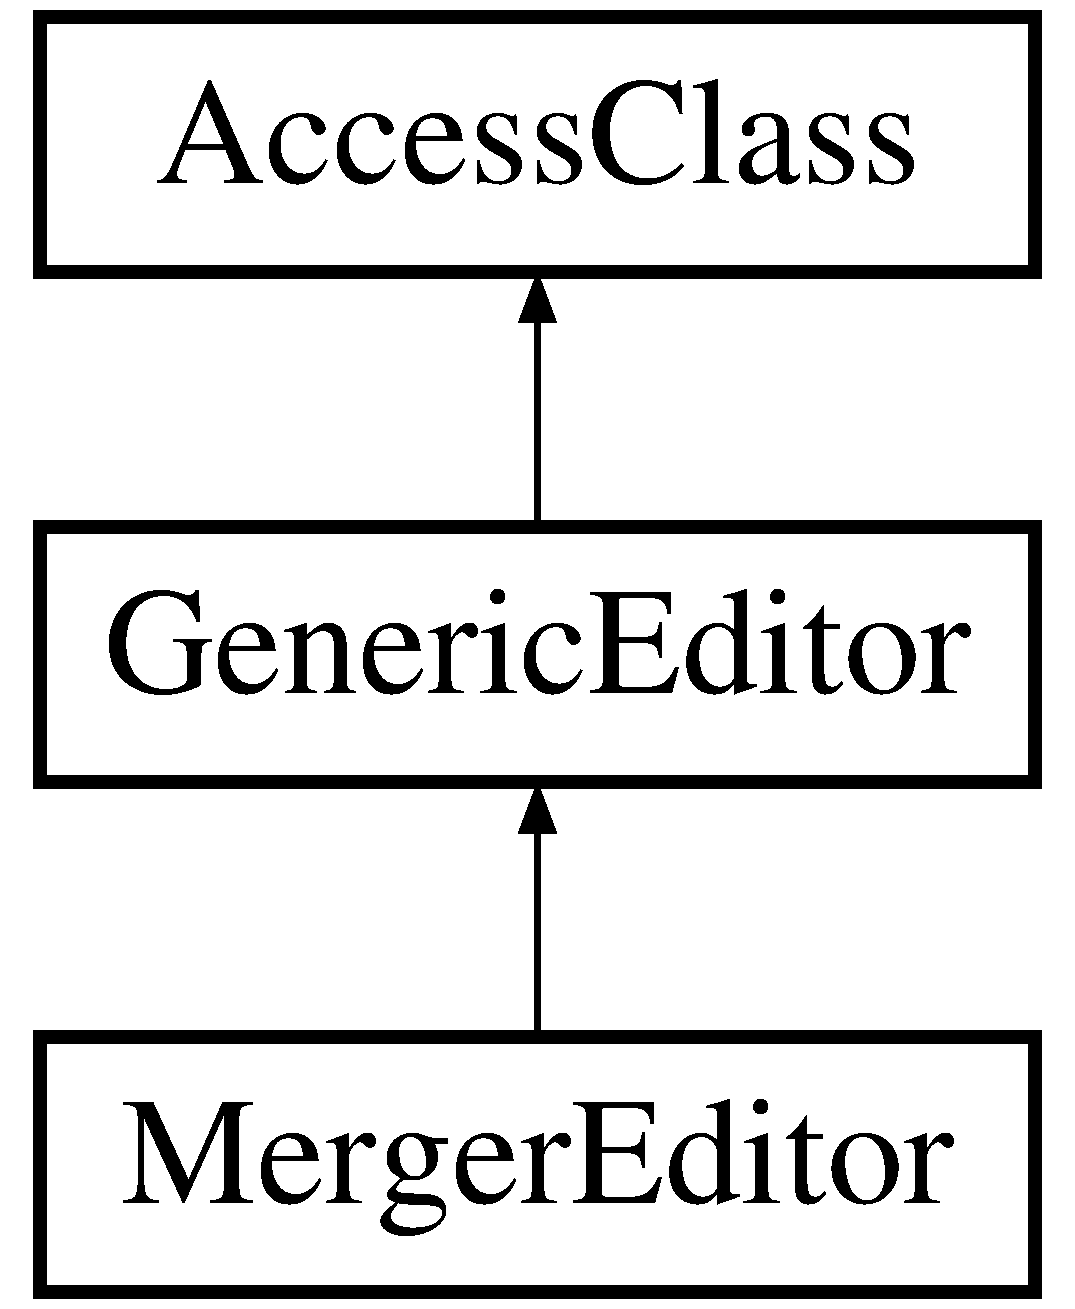
\includegraphics[height=3.000000cm]{classMergerEditor}
\end{center}
\end{figure}
\subsection*{Public Member Functions}
\begin{DoxyCompactItemize}
\item 
\hypertarget{classMergerEditor_a06207ecf36305b3cc68802e7c64aa6b0}{{\bfseries Merger\-Editor} (\hyperlink{classGenericProcessor}{Generic\-Processor} $\ast$parent\-Node)}\label{classMergerEditor_a06207ecf36305b3cc68802e7c64aa6b0}

\item 
\hypertarget{classMergerEditor_a14a01ae643f38d2e677d8fcc72f33d9c}{virtual void {\bfseries button\-Event} (Button $\ast$button)}\label{classMergerEditor_a14a01ae643f38d2e677d8fcc72f33d9c}

\item 
\hypertarget{classMergerEditor_ae31d2de72e81f4cacdc73ebd82d97752}{void {\bfseries switch\-Source} (int)}\label{classMergerEditor_ae31d2de72e81f4cacdc73ebd82d97752}

\item 
\hypertarget{classMergerEditor_af14e4889f12827d50ad517b6cc6d8068}{void {\bfseries switch\-Source} ()}\label{classMergerEditor_af14e4889f12827d50ad517b6cc6d8068}

\item 
\hypertarget{classMergerEditor_a063dd5e128be8ac8e55241966f88c807}{void {\bfseries switch\-I\-O} (int)}\label{classMergerEditor_a063dd5e128be8ac8e55241966f88c807}

\end{DoxyCompactItemize}
\subsection*{Private Member Functions}
\begin{DoxyCompactItemize}
\item 
\hypertarget{classMergerEditor_a20e1c357734a7b7e2851a4838e302e4f}{{\bfseries J\-U\-C\-E\-\_\-\-D\-E\-C\-L\-A\-R\-E\-\_\-\-N\-O\-N\-\_\-\-C\-O\-P\-Y\-A\-B\-L\-E\-\_\-\-W\-I\-T\-H\-\_\-\-L\-E\-A\-K\-\_\-\-D\-E\-T\-E\-C\-T\-O\-R} (\hyperlink{classMergerEditor}{Merger\-Editor})}\label{classMergerEditor_a20e1c357734a7b7e2851a4838e302e4f}

\end{DoxyCompactItemize}
\subsection*{Private Attributes}
\begin{DoxyCompactItemize}
\item 
\hypertarget{classMergerEditor_a5328249601266052a95c2ec88315e151}{Image\-Button $\ast$ {\bfseries pipeline\-Selector\-A}}\label{classMergerEditor_a5328249601266052a95c2ec88315e151}

\item 
\hypertarget{classMergerEditor_aa37ca3add0678985d9b338c421646814}{Image\-Button $\ast$ {\bfseries pipeline\-Selector\-B}}\label{classMergerEditor_aa37ca3add0678985d9b338c421646814}

\end{DoxyCompactItemize}
\subsection*{Additional Inherited Members}


The documentation for this class was generated from the following file\-:\begin{DoxyCompactItemize}
\item 
Processors/\-Editors/Merger\-Editor.\-h\end{DoxyCompactItemize}

\hypertarget{classMessageCenter}{\section{Message\-Center Class Reference}
\label{classMessageCenter}\index{Message\-Center@{Message\-Center}}
}


{\ttfamily \#include $<$Message\-Center.\-h$>$}

\subsection*{Public Member Functions}
\begin{DoxyCompactItemize}
\item 
\hypertarget{classMessageCenter_afca5ea751cb84ee12f59115c8221e4fa}{void {\bfseries paint} (Graphics \&g)}\label{classMessageCenter_afca5ea751cb84ee12f59115c8221e4fa}

\end{DoxyCompactItemize}
\subsection*{Private Member Functions}
\begin{DoxyCompactItemize}
\item 
\hypertarget{classMessageCenter_a28c4ab0e94a5d3bc0393d5ecb753ef30}{void {\bfseries resized} ()}\label{classMessageCenter_a28c4ab0e94a5d3bc0393d5ecb753ef30}

\item 
\hypertarget{classMessageCenter_acd9b8596f683f0a6a6e679a1d56ce7da}{void {\bfseries action\-Listener\-Callback} (const String \&message)}\label{classMessageCenter_acd9b8596f683f0a6a6e679a1d56ce7da}

\end{DoxyCompactItemize}
\subsection*{Private Attributes}
\begin{DoxyCompactItemize}
\item 
\hypertarget{classMessageCenter_a3794f59dfc8644c4a8105b027637b70a}{Label $\ast$ {\bfseries message\-Display\-Area}}\label{classMessageCenter_a3794f59dfc8644c4a8105b027637b70a}

\item 
\hypertarget{classMessageCenter_ae70aa66a29d6d56270d5e5063aa7acf0}{Colour {\bfseries message\-Background}}\label{classMessageCenter_ae70aa66a29d6d56270d5e5063aa7acf0}

\end{DoxyCompactItemize}


\subsection{Detailed Description}
Allows the application to display messages to the user.

The \hyperlink{classMessageCenter}{Message\-Center} is located along the bottom left of the application window.

\begin{DoxySeeAlso}{See also}
\hyperlink{classUIComponent}{U\-I\-Component} 
\end{DoxySeeAlso}


The documentation for this class was generated from the following file\-:\begin{DoxyCompactItemize}
\item 
U\-I/Message\-Center.\-h\end{DoxyCompactItemize}

\hypertarget{classMuteButton}{\section{Mute\-Button Class Reference}
\label{classMuteButton}\index{Mute\-Button@{Mute\-Button}}
}


The documentation for this class was generated from the following file\-:\begin{DoxyCompactItemize}
\item 
Processors/\-Editors/Audio\-Editor.\-h\end{DoxyCompactItemize}

\hypertarget{classNetworkThread}{\section{Network\-Thread Class Reference}
\label{classNetworkThread}\index{Network\-Thread@{Network\-Thread}}
}


{\ttfamily \#include $<$Network\-Thread.\-h$>$}

Inheritance diagram for Network\-Thread\-:\begin{figure}[H]
\begin{center}
\leavevmode
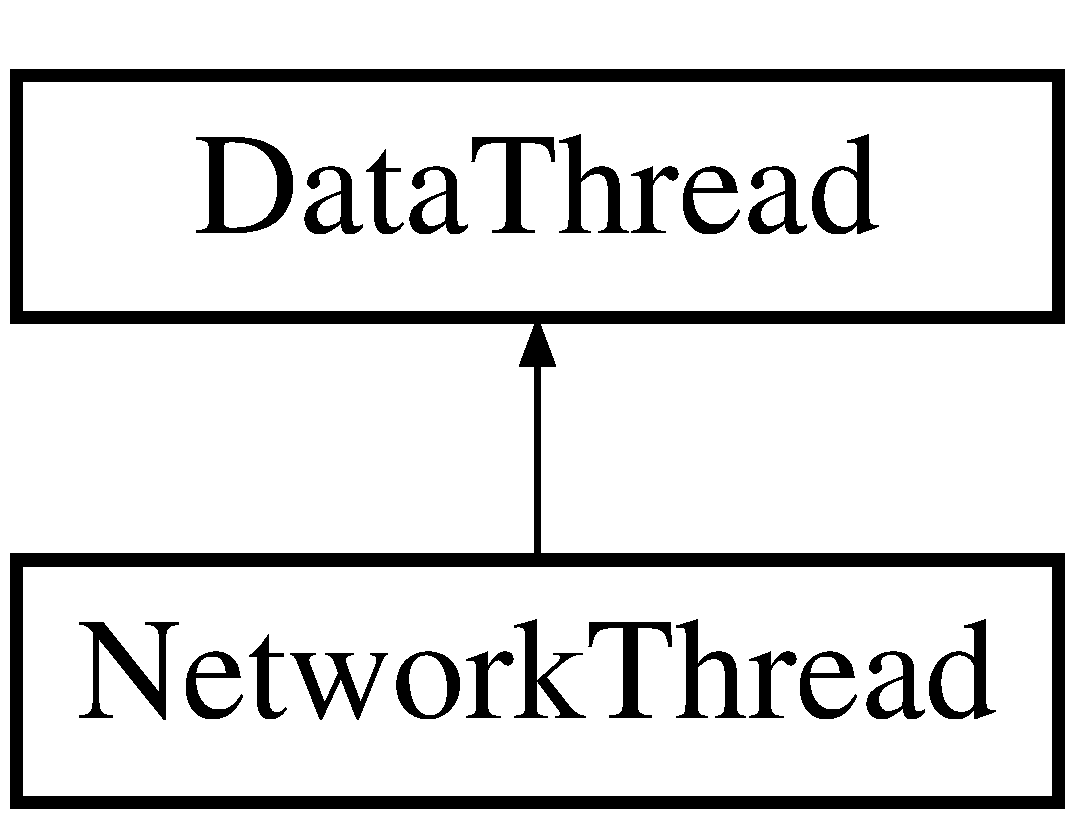
\includegraphics[height=2.000000cm]{classNetworkThread}
\end{center}
\end{figure}
\subsection*{Public Member Functions}
\begin{DoxyCompactItemize}
\item 
\hypertarget{classNetworkThread_adaea87d580354e65bab33405e6e05fe6}{{\bfseries Network\-Thread} (\hyperlink{classSourceNode}{Source\-Node} $\ast$sn)}\label{classNetworkThread_adaea87d580354e65bab33405e6e05fe6}

\item 
\hypertarget{classNetworkThread_a8ded78dab341e5c7c98ccf5fa34f6bb5}{bool {\bfseries found\-Input\-Source} ()}\label{classNetworkThread_a8ded78dab341e5c7c98ccf5fa34f6bb5}

\item 
\hypertarget{classNetworkThread_ae30402dfc01f183929896c07b2efeec5}{bool {\bfseries start\-Acquisition} ()}\label{classNetworkThread_ae30402dfc01f183929896c07b2efeec5}

\item 
\hypertarget{classNetworkThread_a2cc1f3d1e83ab57c2a55657fb6d63956}{bool {\bfseries stop\-Acquisition} ()}\label{classNetworkThread_a2cc1f3d1e83ab57c2a55657fb6d63956}

\item 
\hypertarget{classNetworkThread_a37d244c39c0b0c52882a439638942d40}{int {\bfseries get\-Num\-Channels} ()}\label{classNetworkThread_a37d244c39c0b0c52882a439638942d40}

\item 
\hypertarget{classNetworkThread_a7212f2e4b930e2831e79143bd90b07ab}{float {\bfseries get\-Sample\-Rate} ()}\label{classNetworkThread_a7212f2e4b930e2831e79143bd90b07ab}

\end{DoxyCompactItemize}
\subsection*{Private Member Functions}
\begin{DoxyCompactItemize}
\item 
\hypertarget{classNetworkThread_a7413a18632ce0007e8b11d8d3faf445f}{bool {\bfseries update\-Buffer} ()}\label{classNetworkThread_a7413a18632ce0007e8b11d8d3faf445f}

\item 
\hypertarget{classNetworkThread_af8c35b4c7a7aa9fb8ac251c94489a882}{{\bfseries J\-U\-C\-E\-\_\-\-D\-E\-C\-L\-A\-R\-E\-\_\-\-N\-O\-N\-\_\-\-C\-O\-P\-Y\-A\-B\-L\-E\-\_\-\-W\-I\-T\-H\-\_\-\-L\-E\-A\-K\-\_\-\-D\-E\-T\-E\-C\-T\-O\-R} (\hyperlink{classNetworkThread}{Network\-Thread})}\label{classNetworkThread_af8c35b4c7a7aa9fb8ac251c94489a882}

\end{DoxyCompactItemize}
\subsection*{Private Attributes}
\begin{DoxyCompactItemize}
\item 
\hypertarget{classNetworkThread_a17f457977b6956ed9580cb81047fb7f5}{\hyperlink{classDataBuffer}{Data\-Buffer} $\ast$ {\bfseries data\-Buffer}}\label{classNetworkThread_a17f457977b6956ed9580cb81047fb7f5}

\item 
\hypertarget{classNetworkThread_afd577cd700a51958297d02bb5fda9c9f}{float {\bfseries this\-Sample} \mbox{[}8\mbox{]}}\label{classNetworkThread_afd577cd700a51958297d02bb5fda9c9f}

\end{DoxyCompactItemize}
\subsection*{Additional Inherited Members}


\subsection{Detailed Description}
--O\-B\-S\-O\-L\-E\-T\-E--

Receives data from a network source.

\begin{DoxySeeAlso}{See also}
\hyperlink{classDataThread}{Data\-Thread} 
\end{DoxySeeAlso}


The documentation for this class was generated from the following file\-:\begin{DoxyCompactItemize}
\item 
Processors/\-Data\-Threads/Network\-Thread.\-h\end{DoxyCompactItemize}

\hypertarget{classOpenGLCanvas}{\section{Open\-G\-L\-Canvas Class Reference}
\label{classOpenGLCanvas}\index{Open\-G\-L\-Canvas@{Open\-G\-L\-Canvas}}
}
Inheritance diagram for Open\-G\-L\-Canvas\-:\begin{figure}[H]
\begin{center}
\leavevmode
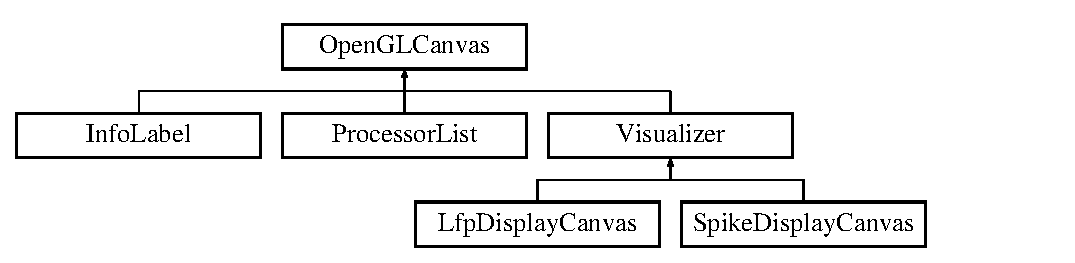
\includegraphics[height=3.000000cm]{classOpenGLCanvas}
\end{center}
\end{figure}
\subsection*{Public Member Functions}
\begin{DoxyCompactItemize}
\item 
\hypertarget{classOpenGLCanvas_a4e5465af99da8ef948080780056e123e}{void {\bfseries set\-Up2\-D\-Canvas} ()}\label{classOpenGLCanvas_a4e5465af99da8ef948080780056e123e}

\item 
\hypertarget{classOpenGLCanvas_a4ce8932a473332c5c651f4f1cd0e0011}{void {\bfseries activate\-Anti\-Aliasing} ()}\label{classOpenGLCanvas_a4ce8932a473332c5c651f4f1cd0e0011}

\item 
\hypertarget{classOpenGLCanvas_adcedeaa60cb0e63d9d595789833c39e3}{virtual void {\bfseries refresh\-State} ()}\label{classOpenGLCanvas_adcedeaa60cb0e63d9d595789833c39e3}

\item 
\hypertarget{classOpenGLCanvas_ae84b5f2f607282735c772d2ceb7a3216}{void {\bfseries resized} ()}\label{classOpenGLCanvas_ae84b5f2f607282735c772d2ceb7a3216}

\item 
\hypertarget{classOpenGLCanvas_a185d4885860a66db22099d44b1e610ed}{virtual void {\bfseries canvas\-Was\-Resized} ()}\label{classOpenGLCanvas_a185d4885860a66db22099d44b1e610ed}

\item 
\hypertarget{classOpenGLCanvas_ac99c34fbaef2b2a045aaf9e494f3bee6}{void {\bfseries mouse\-Down} (const Mouse\-Event \&e)}\label{classOpenGLCanvas_ac99c34fbaef2b2a045aaf9e494f3bee6}

\item 
\hypertarget{classOpenGLCanvas_ac151422c650b9b8fffdd8d046d2721d3}{void {\bfseries mouse\-Drag} (const Mouse\-Event \&e)}\label{classOpenGLCanvas_ac151422c650b9b8fffdd8d046d2721d3}

\item 
\hypertarget{classOpenGLCanvas_a2da895f0e19af911ffce8d8f6ddaecd9}{void {\bfseries mouse\-Move} (const Mouse\-Event \&e)}\label{classOpenGLCanvas_a2da895f0e19af911ffce8d8f6ddaecd9}

\item 
\hypertarget{classOpenGLCanvas_a851ff2424c5b506b0e0f6c7e267fd64a}{void {\bfseries mouse\-Up} (const Mouse\-Event \&e)}\label{classOpenGLCanvas_a851ff2424c5b506b0e0f6c7e267fd64a}

\item 
\hypertarget{classOpenGLCanvas_a8410ec43c862c02fe919eb865aeae0e2}{void {\bfseries mouse\-Wheel\-Move} (const Mouse\-Event \&, float, float)}\label{classOpenGLCanvas_a8410ec43c862c02fe919eb865aeae0e2}

\item 
\hypertarget{classOpenGLCanvas_aee6d5b6ad361deb3ee1b13dbe7715532}{virtual void {\bfseries mouse\-Down\-In\-Canvas} (const Mouse\-Event \&e)}\label{classOpenGLCanvas_aee6d5b6ad361deb3ee1b13dbe7715532}

\item 
\hypertarget{classOpenGLCanvas_a5068fe5a0f604c861f398aab4c319a8d}{virtual void {\bfseries mouse\-Drag\-In\-Canvas} (const Mouse\-Event \&e)}\label{classOpenGLCanvas_a5068fe5a0f604c861f398aab4c319a8d}

\item 
\hypertarget{classOpenGLCanvas_a2f734d31278c4f4443bd2b039bc1a565}{virtual void {\bfseries mouse\-Move\-In\-Canvas} (const Mouse\-Event \&e)}\label{classOpenGLCanvas_a2f734d31278c4f4443bd2b039bc1a565}

\item 
\hypertarget{classOpenGLCanvas_ad39cc41b017720832f7e426e43e54082}{virtual void {\bfseries mouse\-Up\-In\-Canvas} (const Mouse\-Event \&e)}\label{classOpenGLCanvas_ad39cc41b017720832f7e426e43e54082}

\item 
\hypertarget{classOpenGLCanvas_abbf0f5d0407286e3d218efe97a818289}{virtual void {\bfseries mouse\-Wheel\-Move\-In\-Canvas} (const Mouse\-Event \&, float, float)}\label{classOpenGLCanvas_abbf0f5d0407286e3d218efe97a818289}

\item 
\hypertarget{classOpenGLCanvas_aec665b76f2b0578853482762efbd9712}{void {\bfseries start\-Callbacks} ()}\label{classOpenGLCanvas_aec665b76f2b0578853482762efbd9712}

\item 
\hypertarget{classOpenGLCanvas_a8566b4cd2548284e62127d456b76ef46}{void {\bfseries stop\-Callbacks} ()}\label{classOpenGLCanvas_a8566b4cd2548284e62127d456b76ef46}

\item 
\hypertarget{classOpenGLCanvas_a37391e2d630954b0bf1c4d668fc6fca2}{int {\bfseries get\-Scroll\-Amount} ()}\label{classOpenGLCanvas_a37391e2d630954b0bf1c4d668fc6fca2}

\item 
\hypertarget{classOpenGLCanvas_ae8977529a53d1684048e7544cd10f7cd}{int {\bfseries get\-Scroll\-Bar\-Width} ()}\label{classOpenGLCanvas_ae8977529a53d1684048e7544cd10f7cd}

\item 
\hypertarget{classOpenGLCanvas_a55f0ace5fb7461fa9eda94f2bd15b717}{void {\bfseries draw\-Scroll\-Bars} ()}\label{classOpenGLCanvas_a55f0ace5fb7461fa9eda94f2bd15b717}

\item 
\hypertarget{classOpenGLCanvas_afcbdde80a35a50b717b4205642cead9c}{void {\bfseries draw\-Rounded\-Rect} (float x, float y, float w, float h, float r, int n)}\label{classOpenGLCanvas_afcbdde80a35a50b717b4205642cead9c}

\item 
\hypertarget{classOpenGLCanvas_af0d4f85ca66ce079a2b098868f49dc04}{F\-T\-G\-L\-Pixmap\-Font $\ast$ {\bfseries get\-Font} (String font\-Name)}\label{classOpenGLCanvas_af0d4f85ca66ce079a2b098868f49dc04}

\end{DoxyCompactItemize}
\subsection*{Protected Member Functions}
\begin{DoxyCompactItemize}
\item 
\hypertarget{classOpenGLCanvas_a68baeb2eb35fb41ad89dbfc55e8a007e}{virtual int {\bfseries get\-Total\-Height} ()=0}\label{classOpenGLCanvas_a68baeb2eb35fb41ad89dbfc55e8a007e}

\item 
\hypertarget{classOpenGLCanvas_a0cb901644481e0328d043011ea3f1af6}{void {\bfseries show\-Scroll\-Bars} ()}\label{classOpenGLCanvas_a0cb901644481e0328d043011ea3f1af6}

\end{DoxyCompactItemize}
\subsection*{Protected Attributes}
\begin{DoxyCompactItemize}
\item 
\hypertarget{classOpenGLCanvas_a5bf50c5ef28423e92e8e22b2d7beb60b}{int {\bfseries scroll\-Pix}}\label{classOpenGLCanvas_a5bf50c5ef28423e92e8e22b2d7beb60b}

\item 
\hypertarget{classOpenGLCanvas_a48925b61ea3317a3847909ba2c827cc7}{bool {\bfseries animation\-Is\-Active}}\label{classOpenGLCanvas_a48925b61ea3317a3847909ba2c827cc7}

\end{DoxyCompactItemize}
\subsection*{Private Member Functions}
\begin{DoxyCompactItemize}
\item 
\hypertarget{classOpenGLCanvas_a5bc0ce35efc400e7fdd133be03a8b54a}{void {\bfseries load\-Fonts} ()}\label{classOpenGLCanvas_a5bc0ce35efc400e7fdd133be03a8b54a}

\item 
\hypertarget{classOpenGLCanvas_a10b8b42f2bcaabf2ac7c44026bb83d9a}{void {\bfseries draw\-Scroll\-Bar} (float y1, float y2, float alpha)}\label{classOpenGLCanvas_a10b8b42f2bcaabf2ac7c44026bb83d9a}

\item 
\hypertarget{classOpenGLCanvas_ab74dc4155e9207ea7141ca10a980212f}{void {\bfseries timer\-Callback} ()}\label{classOpenGLCanvas_ab74dc4155e9207ea7141ca10a980212f}

\item 
\hypertarget{classOpenGLCanvas_a800f34228a031ebc4034ba5f1cf034bb}{{\bfseries J\-U\-C\-E\-\_\-\-D\-E\-C\-L\-A\-R\-E\-\_\-\-N\-O\-N\-\_\-\-C\-O\-P\-Y\-A\-B\-L\-E\-\_\-\-W\-I\-T\-H\-\_\-\-L\-E\-A\-K\-\_\-\-D\-E\-T\-E\-C\-T\-O\-R} (\hyperlink{classOpenGLCanvas}{Open\-G\-L\-Canvas})}\label{classOpenGLCanvas_a800f34228a031ebc4034ba5f1cf034bb}

\end{DoxyCompactItemize}
\subsection*{Private Attributes}
\begin{DoxyCompactItemize}
\item 
\hypertarget{classOpenGLCanvas_a909b27627ae036d62b60ab63a543b330}{int {\bfseries refresh\-Ms}}\label{classOpenGLCanvas_a909b27627ae036d62b60ab63a543b330}

\item 
\hypertarget{classOpenGLCanvas_a6293f4a62ec535fa57f371481c9df4dd}{int {\bfseries scroll\-Bar\-Width}}\label{classOpenGLCanvas_a6293f4a62ec535fa57f371481c9df4dd}

\item 
\hypertarget{classOpenGLCanvas_a0ada22b76e338a5bfbd30f701098d012}{int {\bfseries scroll\-Diff}}\label{classOpenGLCanvas_a0ada22b76e338a5bfbd30f701098d012}

\item 
\hypertarget{classOpenGLCanvas_a5e8dc9683a6903282827f51d762d077a}{int {\bfseries original\-Scroll\-Pix}}\label{classOpenGLCanvas_a5e8dc9683a6903282827f51d762d077a}

\item 
\hypertarget{classOpenGLCanvas_a275e1d0b1c3e6d96307c7fd836866a61}{int {\bfseries scroll\-Time}}\label{classOpenGLCanvas_a275e1d0b1c3e6d96307c7fd836866a61}

\item 
\hypertarget{classOpenGLCanvas_a5dd720a68dd006d4659048dce18b142e}{bool {\bfseries show\-Scroll\-Track}}\label{classOpenGLCanvas_a5dd720a68dd006d4659048dce18b142e}

\item 
\hypertarget{classOpenGLCanvas_a20554e3f03d0684e098d81ea32c48546}{Time $\ast$ {\bfseries timer}}\label{classOpenGLCanvas_a20554e3f03d0684e098d81ea32c48546}

\item 
\hypertarget{classOpenGLCanvas_aec887b0202c094a8aa5407148ba952c3}{float {\bfseries scroll\-Bar\-Top}}\label{classOpenGLCanvas_aec887b0202c094a8aa5407148ba952c3}

\item 
\hypertarget{classOpenGLCanvas_a4efba8234e1e3f49889ca6d07985b1c2}{float {\bfseries scroll\-Bar\-Bottom}}\label{classOpenGLCanvas_a4efba8234e1e3f49889ca6d07985b1c2}

\item 
\hypertarget{classOpenGLCanvas_ac632b87dc48d1f446d94ebfced6f5dc0}{Owned\-Array$<$ F\-T\-G\-L\-Pixmap\-Font $>$ {\bfseries font\-List}}\label{classOpenGLCanvas_ac632b87dc48d1f446d94ebfced6f5dc0}

\item 
\hypertarget{classOpenGLCanvas_ac48e05ebd99775d76c5dc4c6838dfe04}{const float {\bfseries P\-I}}\label{classOpenGLCanvas_ac48e05ebd99775d76c5dc4c6838dfe04}

\end{DoxyCompactItemize}


The documentation for this class was generated from the following file\-:\begin{DoxyCompactItemize}
\item 
Processors/\-Visualization/Open\-G\-L\-Canvas.\-h\end{DoxyCompactItemize}

\hypertarget{classParameter}{\section{Parameter Class Reference}
\label{classParameter}\index{Parameter@{Parameter}}
}


{\ttfamily \#include $<$Parameter.\-h$>$}

\subsection*{Public Member Functions}
\begin{DoxyCompactItemize}
\item 
\hypertarget{classParameter_a21c5d8266e270b1f23295eabbe35d37f}{{\bfseries Parameter} (const String \&name\-\_\-, bool default\-Val, int I\-D)}\label{classParameter_a21c5d8266e270b1f23295eabbe35d37f}

\item 
\hypertarget{classParameter_a2ee8423ed28378b77eff4e69ebe31be1}{{\bfseries Parameter} (const String \&name\-\_\-, float low, float high, float default\-Val, int I\-D)}\label{classParameter_a2ee8423ed28378b77eff4e69ebe31be1}

\item 
\hypertarget{classParameter_a481767bd518c8c75459dc16580b19199}{{\bfseries Parameter} (const String \&name\-\_\-, Array$<$ var $>$ a, int default\-Val, int I\-D)}\label{classParameter_a481767bd518c8c75459dc16580b19199}

\item 
\hypertarget{classParameter_a40dd77acd828bd3f50832548ec3b8cfd}{const String \& {\bfseries get\-Name} ()}\label{classParameter_a40dd77acd828bd3f50832548ec3b8cfd}

\item 
\hypertarget{classParameter_ad2a916413e8cf95f677a5f2e12ddb919}{const String \& {\bfseries get\-Description} ()}\label{classParameter_ad2a916413e8cf95f677a5f2e12ddb919}

\item 
\hypertarget{classParameter_a2e5de29da44e4d0f04a236c862cce2dc}{void {\bfseries add\-Description} (const String \&desc)}\label{classParameter_a2e5de29da44e4d0f04a236c862cce2dc}

\item 
\hypertarget{classParameter_a6ce1f8114743d115e7d697d186a07f3b}{var {\bfseries get\-Default\-Value} ()}\label{classParameter_a6ce1f8114743d115e7d697d186a07f3b}

\item 
\hypertarget{classParameter_ac26fceaf830c0a9d8378fcb1266a6895}{int {\bfseries get\-I\-D} ()}\label{classParameter_ac26fceaf830c0a9d8378fcb1266a6895}

\item 
\hypertarget{classParameter_a9c111935ac7686c6d553e8cbfdcd6586}{Array$<$ var $>$ {\bfseries get\-Possible\-Values} ()}\label{classParameter_a9c111935ac7686c6d553e8cbfdcd6586}

\item 
\hypertarget{classParameter_a8e5409218cb787ff761c69ca9f77c438}{void {\bfseries set\-Value} (float val, int chan)}\label{classParameter_a8e5409218cb787ff761c69ca9f77c438}

\item 
\hypertarget{classParameter_a62dcb99c0702e094dab71655d5d7fed8}{var {\bfseries operator\mbox{[}$\,$\mbox{]}} (int chan)}\label{classParameter_a62dcb99c0702e094dab71655d5d7fed8}

\item 
\hypertarget{classParameter_a1f27fe3b3fc432f646d0c5244f495b8d}{\hyperlink{classParameter}{Parameter} \& {\bfseries operator=} (const \hyperlink{classParameter}{Parameter} \&other)}\label{classParameter_a1f27fe3b3fc432f646d0c5244f495b8d}

\item 
\hypertarget{classParameter_a0c25100815bda4ae19801fc146529535}{bool {\bfseries is\-Boolean} ()}\label{classParameter_a0c25100815bda4ae19801fc146529535}

\item 
\hypertarget{classParameter_a022c66a8409c6456f9b2d8a3465f0560}{bool {\bfseries is\-Continuous} ()}\label{classParameter_a022c66a8409c6456f9b2d8a3465f0560}

\item 
\hypertarget{classParameter_ac048c296eaaad1d1b168875c932b5681}{bool {\bfseries is\-Discrete} ()}\label{classParameter_ac048c296eaaad1d1b168875c932b5681}

\end{DoxyCompactItemize}
\subsection*{Private Attributes}
\begin{DoxyCompactItemize}
\item 
\hypertarget{classParameter_a18c92c8190d681c49fc6ff60f94245b6}{const String {\bfseries name}}\label{classParameter_a18c92c8190d681c49fc6ff60f94245b6}

\item 
\hypertarget{classParameter_a5aacdf5c58652cc6840ebfbe2a748d29}{String {\bfseries description}}\label{classParameter_a5aacdf5c58652cc6840ebfbe2a748d29}

\item 
\hypertarget{classParameter_ab06e79287bec9288210c65cd6f623851}{int {\bfseries parameter\-Id}}\label{classParameter_ab06e79287bec9288210c65cd6f623851}

\item 
\hypertarget{classParameter_a5006ffe49af0534876d7e6e1fc63d1db}{bool {\bfseries is\-Bool}}\label{classParameter_a5006ffe49af0534876d7e6e1fc63d1db}

\item 
\hypertarget{classParameter_a33f6f455be804dbc9743d7b9124bc1e4}{bool {\bfseries is\-Cont}}\label{classParameter_a33f6f455be804dbc9743d7b9124bc1e4}

\item 
\hypertarget{classParameter_afceec950c5fa0b6968dd87bc6a652740}{bool {\bfseries is\-Disc}}\label{classParameter_afceec950c5fa0b6968dd87bc6a652740}

\item 
\hypertarget{classParameter_a7876f41120778114b3c61671e8531c05}{var {\bfseries default\-Value}}\label{classParameter_a7876f41120778114b3c61671e8531c05}

\item 
\hypertarget{classParameter_a75745989a25c8ef2b3c6d25bc22963c4}{Array$<$ var $>$ {\bfseries values}}\label{classParameter_a75745989a25c8ef2b3c6d25bc22963c4}

\item 
\hypertarget{classParameter_a67fc656af78ffe47e4cdefc99bc21e91}{Array$<$ var $>$ {\bfseries possible\-Values}}\label{classParameter_a67fc656af78ffe47e4cdefc99bc21e91}

\end{DoxyCompactItemize}


\subsection{Detailed Description}
Class for holding user-\/definable processor parameters.

\begin{DoxySeeAlso}{See also}
\hyperlink{classGenericProcessor}{Generic\-Processor}, \hyperlink{classGenericEditor}{Generic\-Editor} 
\end{DoxySeeAlso}


The documentation for this class was generated from the following file\-:\begin{DoxyCompactItemize}
\item 
Processors/Parameter.\-h\end{DoxyCompactItemize}

\hypertarget{classParameterButton}{\section{Parameter\-Button Class Reference}
\label{classParameterButton}\index{Parameter\-Button@{Parameter\-Button}}
}
\subsection*{Public Member Functions}
\begin{DoxyCompactItemize}
\item 
\hypertarget{classParameterButton_a7a59b296f37ce92795e3017d56dd8bcd}{{\bfseries Parameter\-Button} (var value, int button\-Type, Font label\-Font)}\label{classParameterButton_a7a59b296f37ce92795e3017d56dd8bcd}

\end{DoxyCompactItemize}
\subsection*{Private Types}
\begin{DoxyCompactItemize}
\item 
enum \{ {\bfseries L\-E\-F\-T}, 
{\bfseries M\-I\-D\-D\-L\-E}, 
{\bfseries R\-I\-G\-H\-T}
 \}
\end{DoxyCompactItemize}
\subsection*{Private Member Functions}
\begin{DoxyCompactItemize}
\item 
\hypertarget{classParameterButton_a22a9563ef2a093d9cb7afea8d3d9356d}{void {\bfseries paint\-Button} (Graphics \&g, bool is\-Mouse\-Over, bool is\-Button\-Down)}\label{classParameterButton_a22a9563ef2a093d9cb7afea8d3d9356d}

\item 
\hypertarget{classParameterButton_a36fb863b412ede301507f9fe2fb01614}{void {\bfseries resized} ()}\label{classParameterButton_a36fb863b412ede301507f9fe2fb01614}

\end{DoxyCompactItemize}
\subsection*{Private Attributes}
\begin{DoxyCompactItemize}
\item 
\hypertarget{classParameterButton_a55676c2d0264727d097514ce4be4bb67}{int {\bfseries type}}\label{classParameterButton_a55676c2d0264727d097514ce4be4bb67}

\item 
\hypertarget{classParameterButton_a22bda9a20291345d25e2402d8e1e7837}{Path {\bfseries outline\-Path}}\label{classParameterButton_a22bda9a20291345d25e2402d8e1e7837}

\item 
\hypertarget{classParameterButton_ad71f8a5d0b0ad16923b0f29c78cc17ad}{const String {\bfseries value\-String}}\label{classParameterButton_ad71f8a5d0b0ad16923b0f29c78cc17ad}

\item 
\hypertarget{classParameterButton_ab7554783d5d6864ea8facb93db1ab1fc}{Font {\bfseries font}}\label{classParameterButton_ab7554783d5d6864ea8facb93db1ab1fc}

\item 
\hypertarget{classParameterButton_a0bcf00e16032a383e93a87a633959e1e}{Colour\-Gradient {\bfseries selected\-Grad}}\label{classParameterButton_a0bcf00e16032a383e93a87a633959e1e}

\item 
\hypertarget{classParameterButton_a2efe962907ce0355310f58ff2d1320fc}{Colour\-Gradient {\bfseries selected\-Over\-Grad}}\label{classParameterButton_a2efe962907ce0355310f58ff2d1320fc}

\item 
\hypertarget{classParameterButton_a3b547b9434b12999f741babbb5c855f2}{Colour\-Gradient {\bfseries neutral\-Grad}}\label{classParameterButton_a3b547b9434b12999f741babbb5c855f2}

\item 
\hypertarget{classParameterButton_a1e2978b82beada5f5e9881619399efdb}{Colour\-Gradient {\bfseries neutral\-Over\-Grad}}\label{classParameterButton_a1e2978b82beada5f5e9881619399efdb}

\end{DoxyCompactItemize}


The documentation for this class was generated from the following file\-:\begin{DoxyCompactItemize}
\item 
Processors/\-Editors/Parameter\-Editor.\-h\end{DoxyCompactItemize}

\hypertarget{classParameterCheckbox}{\section{Parameter\-Checkbox Class Reference}
\label{classParameterCheckbox}\index{Parameter\-Checkbox@{Parameter\-Checkbox}}
}
\subsection*{Public Member Functions}
\begin{DoxyCompactItemize}
\item 
\hypertarget{classParameterCheckbox_a0cbf41733b9adf5c052a6191471a3bf1}{{\bfseries Parameter\-Checkbox} (bool default\-State)}\label{classParameterCheckbox_a0cbf41733b9adf5c052a6191471a3bf1}

\end{DoxyCompactItemize}
\subsection*{Private Member Functions}
\begin{DoxyCompactItemize}
\item 
\hypertarget{classParameterCheckbox_a5c4f3c9168930acba05420d73eef27d7}{void {\bfseries paint\-Button} (Graphics \&g, bool is\-Mouse\-Over, bool is\-Button\-Down)}\label{classParameterCheckbox_a5c4f3c9168930acba05420d73eef27d7}

\end{DoxyCompactItemize}
\subsection*{Private Attributes}
\begin{DoxyCompactItemize}
\item 
\hypertarget{classParameterCheckbox_ac5c3d91e3a6d989d5221f47c36174823}{Colour\-Gradient {\bfseries selected\-Grad}}\label{classParameterCheckbox_ac5c3d91e3a6d989d5221f47c36174823}

\item 
\hypertarget{classParameterCheckbox_a3176afbf0afc9747b3a8eae6d03515e7}{Colour\-Gradient {\bfseries selected\-Over\-Grad}}\label{classParameterCheckbox_a3176afbf0afc9747b3a8eae6d03515e7}

\item 
\hypertarget{classParameterCheckbox_a0a1063e260bee5d2cb5e930c498768f7}{Colour\-Gradient {\bfseries neutral\-Grad}}\label{classParameterCheckbox_a0a1063e260bee5d2cb5e930c498768f7}

\item 
\hypertarget{classParameterCheckbox_a38234e37e544e473f48c3e540db1de8f}{Colour\-Gradient {\bfseries neutral\-Over\-Grad}}\label{classParameterCheckbox_a38234e37e544e473f48c3e540db1de8f}

\end{DoxyCompactItemize}


The documentation for this class was generated from the following file\-:\begin{DoxyCompactItemize}
\item 
Processors/\-Editors/Parameter\-Editor.\-h\end{DoxyCompactItemize}

\hypertarget{classParameterEditor}{\section{Parameter\-Editor Class Reference}
\label{classParameterEditor}\index{Parameter\-Editor@{Parameter\-Editor}}
}


{\ttfamily \#include $<$Parameter\-Editor.\-h$>$}

\subsection*{Public Member Functions}
\begin{DoxyCompactItemize}
\item 
\hypertarget{classParameterEditor_a5dc3516d57088e43b2594077abac9229}{{\bfseries Parameter\-Editor} (\hyperlink{classGenericProcessor}{Generic\-Processor} $\ast$proc, \hyperlink{classParameter}{Parameter} \&p, Font label\-Font)}\label{classParameterEditor_a5dc3516d57088e43b2594077abac9229}

\item 
\hypertarget{classParameterEditor_a3642982edfaf45fcd4a75251de47a7d1}{void {\bfseries parent\-Hierarchy\-Changed} ()}\label{classParameterEditor_a3642982edfaf45fcd4a75251de47a7d1}

\item 
\hypertarget{classParameterEditor_aa4cc89334e9f4060253a68854ffbf6a5}{void {\bfseries button\-Clicked} (Button $\ast$button)}\label{classParameterEditor_aa4cc89334e9f4060253a68854ffbf6a5}

\item 
\hypertarget{classParameterEditor_a4d01772de9fcc90aa059172aac956183}{void {\bfseries slider\-Value\-Changed} (Slider $\ast$slider)}\label{classParameterEditor_a4d01772de9fcc90aa059172aac956183}

\item 
\hypertarget{classParameterEditor_a2bbf1ac9398bb026cb2de2f493ab7c08}{void {\bfseries set\-Channel\-Selector} (\hyperlink{classChannelSelector}{Channel\-Selector} $\ast$ch)}\label{classParameterEditor_a2bbf1ac9398bb026cb2de2f493ab7c08}

\end{DoxyCompactItemize}
\subsection*{Public Attributes}
\begin{DoxyCompactItemize}
\item 
\hypertarget{classParameterEditor_aaf62ff28c11605e190aa098d0af13907}{int {\bfseries desired\-Width}}\label{classParameterEditor_aaf62ff28c11605e190aa098d0af13907}

\item 
\hypertarget{classParameterEditor_a558f492aa13acaef4cd65132fbbcdc9f}{int {\bfseries desired\-Height}}\label{classParameterEditor_a558f492aa13acaef4cd65132fbbcdc9f}

\end{DoxyCompactItemize}
\subsection*{Private Types}
\begin{DoxyCompactItemize}
\item 
enum \{ {\bfseries L\-E\-F\-T}, 
{\bfseries M\-I\-D\-D\-L\-E}, 
{\bfseries R\-I\-G\-H\-T}
 \}
\end{DoxyCompactItemize}
\subsection*{Private Attributes}
\begin{DoxyCompactItemize}
\item 
\hypertarget{classParameterEditor_a32f7ab3ffbe27803677295a51aa15a8e}{Array$<$ Slider $\ast$ $>$ {\bfseries slider\-Array}}\label{classParameterEditor_a32f7ab3ffbe27803677295a51aa15a8e}

\item 
\hypertarget{classParameterEditor_a386d3dd60d24695937c2013a969196c5}{Array$<$ Button $\ast$ $>$ {\bfseries button\-Array}}\label{classParameterEditor_a386d3dd60d24695937c2013a969196c5}

\item 
\hypertarget{classParameterEditor_ad44b9f967fdc823f8d079253dd49744c}{Array$<$ int $>$ {\bfseries button\-Id\-Array}}\label{classParameterEditor_ad44b9f967fdc823f8d079253dd49744c}

\item 
\hypertarget{classParameterEditor_a0b47ca4f8e1b04d8fa0e74f65202af57}{Array$<$ int $>$ {\bfseries slider\-Id\-Array}}\label{classParameterEditor_a0b47ca4f8e1b04d8fa0e74f65202af57}

\item 
\hypertarget{classParameterEditor_ae0cc3f3aa09a4e490891ba4f860544fd}{\hyperlink{classGenericProcessor}{Generic\-Processor} $\ast$ {\bfseries processor}}\label{classParameterEditor_ae0cc3f3aa09a4e490891ba4f860544fd}

\item 
\hypertarget{classParameterEditor_acc6ef739b4229d97fa45d026293296a9}{\hyperlink{classChannelSelector}{Channel\-Selector} $\ast$ {\bfseries channel\-Selector}}\label{classParameterEditor_acc6ef739b4229d97fa45d026293296a9}

\end{DoxyCompactItemize}


\subsection{Detailed Description}
Automatically creates an interactive editor for a particular parameter.

\begin{DoxySeeAlso}{See also}
\hyperlink{classGenericEditor}{Generic\-Editor}, \hyperlink{classGenericProcessor}{Generic\-Processor}, \hyperlink{classParameter}{Parameter} 
\end{DoxySeeAlso}


The documentation for this class was generated from the following file\-:\begin{DoxyCompactItemize}
\item 
Processors/\-Editors/Parameter\-Editor.\-h\end{DoxyCompactItemize}

\hypertarget{classParameterSlider}{\section{Parameter\-Slider Class Reference}
\label{classParameterSlider}\index{Parameter\-Slider@{Parameter\-Slider}}
}
\subsection*{Public Member Functions}
\begin{DoxyCompactItemize}
\item 
\hypertarget{classParameterSlider_a545597c0f64eda6cb2ddb1f07d21eb4d}{{\bfseries Parameter\-Slider} (float min, float max, float default\-Value, Font f)}\label{classParameterSlider_a545597c0f64eda6cb2ddb1f07d21eb4d}

\end{DoxyCompactItemize}
\subsection*{Private Member Functions}
\begin{DoxyCompactItemize}
\item 
\hypertarget{classParameterSlider_ae7b164af4b95158aea4afcedcc5462ff}{void {\bfseries paint} (Graphics \&g)}\label{classParameterSlider_ae7b164af4b95158aea4afcedcc5462ff}

\item 
\hypertarget{classParameterSlider_a2624cc7dd3c685231028e3f46a235503}{Path {\bfseries make\-Rotary\-Path} (double, double, double)}\label{classParameterSlider_a2624cc7dd3c685231028e3f46a235503}

\end{DoxyCompactItemize}
\subsection*{Private Attributes}
\begin{DoxyCompactItemize}
\item 
\hypertarget{classParameterSlider_a9131919f5a994ad3815d19e98d7c11c2}{Font {\bfseries font}}\label{classParameterSlider_a9131919f5a994ad3815d19e98d7c11c2}

\end{DoxyCompactItemize}


The documentation for this class was generated from the following file\-:\begin{DoxyCompactItemize}
\item 
Processors/\-Editors/Parameter\-Editor.\-h\end{DoxyCompactItemize}

\hypertarget{classPlayButton}{\section{Play\-Button Class Reference}
\label{classPlayButton}\index{Play\-Button@{Play\-Button}}
}


{\ttfamily \#include $<$Control\-Panel.\-h$>$}



\subsection{Detailed Description}
Displays information and provides buttons to control acquistion and recording.

The \hyperlink{classControlPanel}{Control\-Panel} is located along the top of the application window.

\begin{DoxySeeAlso}{See also}
\hyperlink{classUIComponent}{U\-I\-Component} 
\end{DoxySeeAlso}


The documentation for this class was generated from the following file\-:\begin{DoxyCompactItemize}
\item 
U\-I/Control\-Panel.\-h\end{DoxyCompactItemize}

\hypertarget{classProcessorGraph}{\section{Processor\-Graph Class Reference}
\label{classProcessorGraph}\index{Processor\-Graph@{Processor\-Graph}}
}
Inheritance diagram for Processor\-Graph\-:\begin{figure}[H]
\begin{center}
\leavevmode
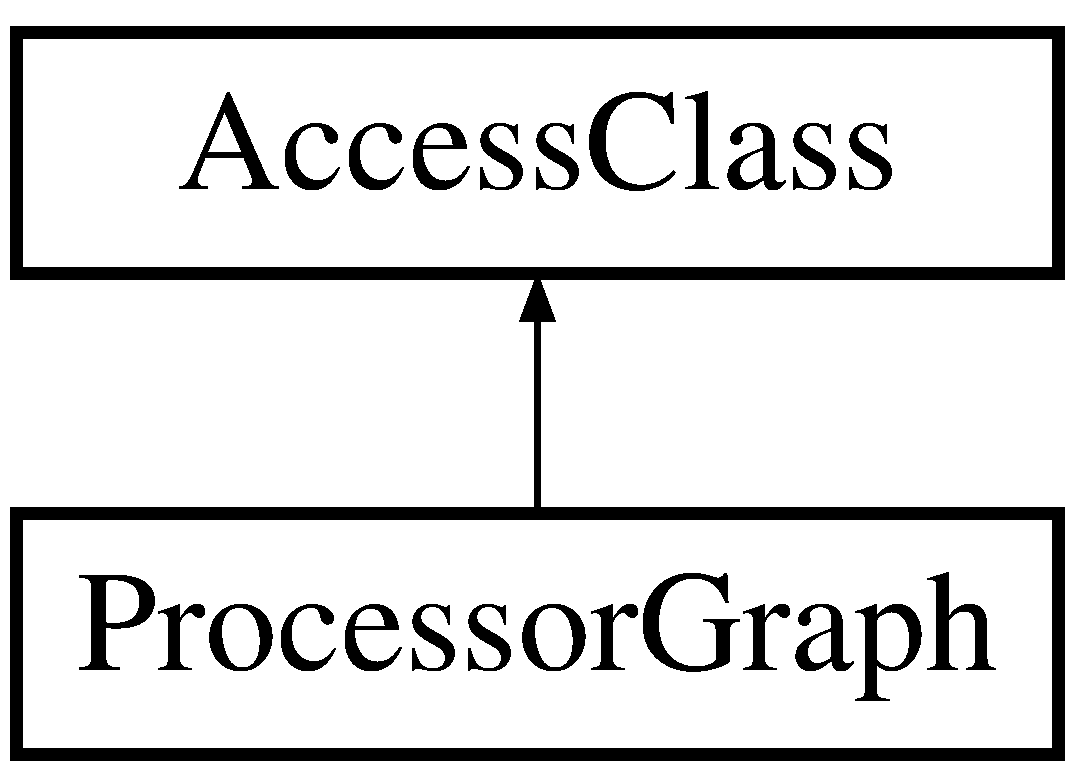
\includegraphics[height=2.000000cm]{classProcessorGraph}
\end{center}
\end{figure}
\subsection*{Public Member Functions}
\begin{DoxyCompactItemize}
\item 
\hypertarget{classProcessorGraph_a75a8c555386eb322aabb83b6cb651f76}{void $\ast$ {\bfseries create\-New\-Processor} (String \&description)}\label{classProcessorGraph_a75a8c555386eb322aabb83b6cb651f76}

\item 
\hypertarget{classProcessorGraph_a91f653d71fcc41eb5ac7976da64be5f5}{\hyperlink{classGenericProcessor}{Generic\-Processor} $\ast$ {\bfseries create\-Processor\-From\-Description} (String \&description)}\label{classProcessorGraph_a91f653d71fcc41eb5ac7976da64be5f5}

\item 
\hypertarget{classProcessorGraph_a3ca938850a4e4f27cae467eeff5046cf}{void {\bfseries remove\-Processor} (\hyperlink{classGenericProcessor}{Generic\-Processor} $\ast$processor)}\label{classProcessorGraph_a3ca938850a4e4f27cae467eeff5046cf}

\item 
\hypertarget{classProcessorGraph_a9affe0a1bddce5272cab547d4c38472a}{void {\bfseries clear\-Signal\-Chain} ()}\label{classProcessorGraph_a9affe0a1bddce5272cab547d4c38472a}

\item 
\hypertarget{classProcessorGraph_acece6f68878404ef8672af84a10e23f3}{bool {\bfseries enable\-Processors} ()}\label{classProcessorGraph_acece6f68878404ef8672af84a10e23f3}

\item 
\hypertarget{classProcessorGraph_a2c0c9688eeaea12a8fe5357b73e58785}{bool {\bfseries disable\-Processors} ()}\label{classProcessorGraph_a2c0c9688eeaea12a8fe5357b73e58785}

\item 
\hypertarget{classProcessorGraph_a1ff73af3414c2329cf1db7d3dc5ccc78}{\hyperlink{classRecordNode}{Record\-Node} $\ast$ {\bfseries get\-Record\-Node} ()}\label{classProcessorGraph_a1ff73af3414c2329cf1db7d3dc5ccc78}

\item 
\hypertarget{classProcessorGraph_af34c4fcdf99f327c922daf6a9e4c9caf}{\hyperlink{classAudioNode}{Audio\-Node} $\ast$ {\bfseries get\-Audio\-Node} ()}\label{classProcessorGraph_af34c4fcdf99f327c922daf6a9e4c9caf}

\item 
\hypertarget{classProcessorGraph_ae183b5807e57ec401d4d3517fc457e2a}{void {\bfseries update\-Connections} (Array$<$ \hyperlink{classSignalChainTabButton}{Signal\-Chain\-Tab\-Button} $\ast$, Critical\-Section $>$)}\label{classProcessorGraph_ae183b5807e57ec401d4d3517fc457e2a}

\item 
\hypertarget{classProcessorGraph_a7ddf86dcf1c88e6da9095396734d560c}{bool {\bfseries processor\-With\-Same\-Name\-Exists} (const String \&name)}\label{classProcessorGraph_a7ddf86dcf1c88e6da9095396734d560c}

\item 
\hypertarget{classProcessorGraph_ae9c9c8963bd984fe099792770a64d596}{void {\bfseries change\-Listener\-Callback} (Change\-Broadcaster $\ast$source)}\label{classProcessorGraph_ae9c9c8963bd984fe099792770a64d596}

\end{DoxyCompactItemize}
\subsection*{Private Types}
\begin{DoxyCompactItemize}
\item 
enum {\bfseries node\-Ids} \{ {\bfseries R\-E\-C\-O\-R\-D\-\_\-\-N\-O\-D\-E\-\_\-\-I\-D} =  900, 
{\bfseries A\-U\-D\-I\-O\-\_\-\-N\-O\-D\-E\-\_\-\-I\-D} =  901, 
{\bfseries O\-U\-T\-P\-U\-T\-\_\-\-N\-O\-D\-E\-\_\-\-I\-D} =  902, 
{\bfseries R\-E\-S\-A\-M\-P\-L\-I\-N\-G\-\_\-\-N\-O\-D\-E\-\_\-\-I\-D} =  903
 \}
\end{DoxyCompactItemize}
\subsection*{Private Member Functions}
\begin{DoxyCompactItemize}
\item 
\hypertarget{classProcessorGraph_a3f10a351d6c862e4496b52a45d69b908}{void {\bfseries create\-Default\-Nodes} ()}\label{classProcessorGraph_a3f10a351d6c862e4496b52a45d69b908}

\item 
\hypertarget{classProcessorGraph_a8a04cdeb5ab26780f2aac2ff3335c6d2}{void {\bfseries clear\-Connections} ()}\label{classProcessorGraph_a8a04cdeb5ab26780f2aac2ff3335c6d2}

\end{DoxyCompactItemize}
\subsection*{Private Attributes}
\begin{DoxyCompactItemize}
\item 
\hypertarget{classProcessorGraph_a680233a4621ccf825cce29625cca6fc0}{int {\bfseries current\-Node\-Id}}\label{classProcessorGraph_a680233a4621ccf825cce29625cca6fc0}

\end{DoxyCompactItemize}


The documentation for this class was generated from the following file\-:\begin{DoxyCompactItemize}
\item 
Processors/Processor\-Graph.\-h\end{DoxyCompactItemize}

\hypertarget{classProcessorList}{\section{Processor\-List Class Reference}
\label{classProcessorList}\index{Processor\-List@{Processor\-List}}
}
Inheritance diagram for Processor\-List\-:\begin{figure}[H]
\begin{center}
\leavevmode
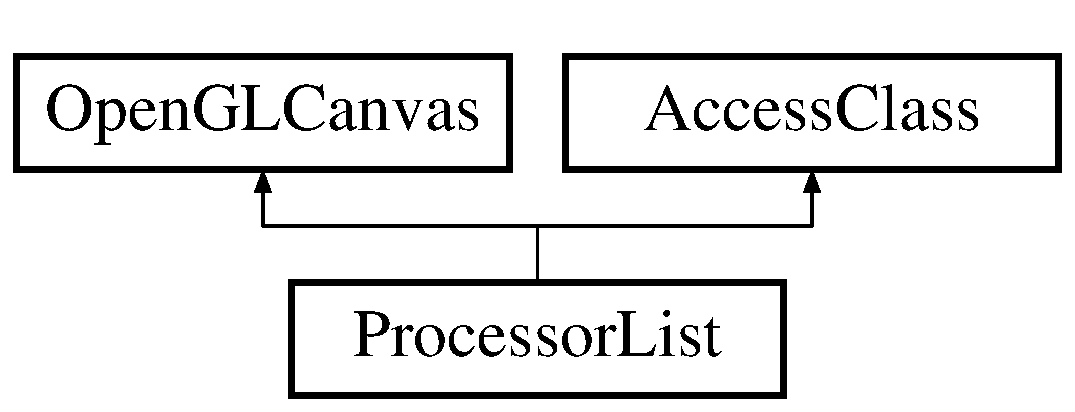
\includegraphics[height=2.000000cm]{classProcessorList}
\end{center}
\end{figure}
\subsection*{Public Member Functions}
\begin{DoxyCompactItemize}
\item 
\hypertarget{classProcessorList_a5ca8297372a8275310b49fab3dc19e87}{void {\bfseries new\-Open\-G\-L\-Context\-Created} ()}\label{classProcessorList_a5ca8297372a8275310b49fab3dc19e87}

\item 
\hypertarget{classProcessorList_affadd35d149f91d659285b2c6481cde6}{void {\bfseries render\-Open\-G\-L} ()}\label{classProcessorList_affadd35d149f91d659285b2c6481cde6}

\item 
\hypertarget{classProcessorList_ae764e342d076a7bc3a3d91b9158b2e79}{void {\bfseries toggle\-State} ()}\label{classProcessorList_ae764e342d076a7bc3a3d91b9158b2e79}

\item 
\hypertarget{classProcessorList_abf7f1a03787844bbbe4866ebe1d858c5}{void {\bfseries change\-Listener\-Callback} (Change\-Broadcaster $\ast$source)}\label{classProcessorList_abf7f1a03787844bbbe4866ebe1d858c5}

\item 
\hypertarget{classProcessorList_ac02cb5b4e006b02e60e37c9f25bdf668}{bool {\bfseries is\-Open} ()}\label{classProcessorList_ac02cb5b4e006b02e60e37c9f25bdf668}

\end{DoxyCompactItemize}
\subsection*{Private Types}
\begin{DoxyCompactItemize}
\item 
enum \{ \\*
{\bfseries P\-R\-O\-C\-E\-S\-S\-O\-R\-\_\-\-C\-O\-L\-O\-R} =  801, 
{\bfseries F\-I\-L\-T\-E\-R\-\_\-\-C\-O\-L\-O\-R} =  802, 
{\bfseries S\-I\-N\-K\-\_\-\-C\-O\-L\-O\-R} =  803, 
{\bfseries S\-O\-U\-R\-C\-E\-\_\-\-C\-O\-L\-O\-R} =  804, 
\\*
{\bfseries U\-T\-I\-L\-I\-T\-Y\-\_\-\-C\-O\-L\-O\-R} =  805
 \}
\end{DoxyCompactItemize}
\subsection*{Private Member Functions}
\begin{DoxyCompactItemize}
\item 
\hypertarget{classProcessorList_a842f29d228a69d183b9b503ebef4cda4}{void {\bfseries draw\-Items} ()}\label{classProcessorList_a842f29d228a69d183b9b503ebef4cda4}

\item 
\hypertarget{classProcessorList_a74d7820267f0275ae81461e7f2c6e29c}{void {\bfseries draw\-Item} (\hyperlink{classProcessorListItem}{Processor\-List\-Item} $\ast$)}\label{classProcessorList_a74d7820267f0275ae81461e7f2c6e29c}

\item 
\hypertarget{classProcessorList_a049a24772e4088a9be29cc9bada12280}{void {\bfseries draw\-Item\-Name} (\hyperlink{classProcessorListItem}{Processor\-List\-Item} $\ast$)}\label{classProcessorList_a049a24772e4088a9be29cc9bada12280}

\item 
\hypertarget{classProcessorList_a20bb75ee2f2543927d4a4caa01f73203}{void {\bfseries draw\-Button} (bool is\-Open)}\label{classProcessorList_a20bb75ee2f2543927d4a4caa01f73203}

\item 
\hypertarget{classProcessorList_a3a2eb03367b34206483307555a0b28f2}{\hyperlink{classProcessorListItem}{Processor\-List\-Item} $\ast$ {\bfseries get\-List\-Item\-For\-Y\-Pos} (int y)}\label{classProcessorList_a3a2eb03367b34206483307555a0b28f2}

\item 
\hypertarget{classProcessorList_a42feb966830ce411e2b6a2ab8a4915b5}{void {\bfseries set\-Viewport} (bool)}\label{classProcessorList_a42feb966830ce411e2b6a2ab8a4915b5}

\item 
\hypertarget{classProcessorList_a0a16364cdfd8d6bf5f706629b325ff84}{int {\bfseries get\-Total\-Height} ()}\label{classProcessorList_a0a16364cdfd8d6bf5f706629b325ff84}

\item 
\hypertarget{classProcessorList_ae5a0d9e43c404e6b5c234c68b65eefb7}{void {\bfseries clear\-Selection\-State} ()}\label{classProcessorList_ae5a0d9e43c404e6b5c234c68b65eefb7}

\item 
\hypertarget{classProcessorList_ad744b9c8c775e77fc1d23194b4e7b93b}{void {\bfseries mouse\-Down\-In\-Canvas} (const Mouse\-Event \&e)}\label{classProcessorList_ad744b9c8c775e77fc1d23194b4e7b93b}

\item 
\hypertarget{classProcessorList_a2597d2a52f8ec19d4ee8a2633e6c4b51}{void {\bfseries mouse\-Drag\-In\-Canvas} (const Mouse\-Event \&e)}\label{classProcessorList_a2597d2a52f8ec19d4ee8a2633e6c4b51}

\item 
\hypertarget{classProcessorList_a44cc07fd66600b293ade3b958350bc62}{{\bfseries J\-U\-C\-E\-\_\-\-D\-E\-C\-L\-A\-R\-E\-\_\-\-N\-O\-N\-\_\-\-C\-O\-P\-Y\-A\-B\-L\-E\-\_\-\-W\-I\-T\-H\-\_\-\-L\-E\-A\-K\-\_\-\-D\-E\-T\-E\-C\-T\-O\-R} (\hyperlink{classProcessorList}{Processor\-List})}\label{classProcessorList_a44cc07fd66600b293ade3b958350bc62}

\end{DoxyCompactItemize}
\subsection*{Private Attributes}
\begin{DoxyCompactItemize}
\item 
\hypertarget{classProcessorList_aa15bd6fc784ec300c409591d85dc1e72}{int {\bfseries current\-Color}}\label{classProcessorList_aa15bd6fc784ec300c409591d85dc1e72}

\item 
\hypertarget{classProcessorList_a1a341a670be20804eabb72c492b684a8}{bool {\bfseries is\-Dragging}}\label{classProcessorList_a1a341a670be20804eabb72c492b684a8}

\item 
\hypertarget{classProcessorList_a1284c3fdf5c05e58526791b4691a7c5c}{int {\bfseries total\-Height}}\label{classProcessorList_a1284c3fdf5c05e58526791b4691a7c5c}

\item 
\hypertarget{classProcessorList_a98d0271bd20252eb763df33cb2ce7867}{int {\bfseries item\-Height}}\label{classProcessorList_a98d0271bd20252eb763df33cb2ce7867}

\item 
\hypertarget{classProcessorList_af0d75f66b3b90d78db99601a69a01591}{int {\bfseries sub\-Item\-Height}}\label{classProcessorList_af0d75f66b3b90d78db99601a69a01591}

\item 
\hypertarget{classProcessorList_a7976c45e018552716dd6eba492f6b997}{int {\bfseries x\-Buffer}}\label{classProcessorList_a7976c45e018552716dd6eba492f6b997}

\item 
\hypertarget{classProcessorList_a7ff6a5a231f7b5a9f7b279334f1bd3db}{int {\bfseries y\-Buffer}}\label{classProcessorList_a7ff6a5a231f7b5a9f7b279334f1bd3db}

\item 
\hypertarget{classProcessorList_a7500fdcc9425b0bca0c2f53df2491a06}{String {\bfseries category}}\label{classProcessorList_a7500fdcc9425b0bca0c2f53df2491a06}

\item 
\hypertarget{classProcessorList_a9bd614bdd6198da16c8af8e120278912}{\hyperlink{classProcessorListItem}{Processor\-List\-Item} $\ast$ {\bfseries base\-Item}}\label{classProcessorList_a9bd614bdd6198da16c8af8e120278912}

\end{DoxyCompactItemize}
\subsection*{Additional Inherited Members}


The documentation for this class was generated from the following file\-:\begin{DoxyCompactItemize}
\item 
U\-I/Processor\-List.\-h\end{DoxyCompactItemize}

\hypertarget{classProcessorListItem}{\section{Processor\-List\-Item Class Reference}
\label{classProcessorListItem}\index{Processor\-List\-Item@{Processor\-List\-Item}}
}
\subsection*{Public Member Functions}
\begin{DoxyCompactItemize}
\item 
\hypertarget{classProcessorListItem_a6089a302cb290dead024ad158ae8e28f}{{\bfseries Processor\-List\-Item} (const String \&name)}\label{classProcessorListItem_a6089a302cb290dead024ad158ae8e28f}

\item 
\hypertarget{classProcessorListItem_ad783cc2b23fcebf02e905675c681a585}{int {\bfseries get\-Num\-Sub\-Items} ()}\label{classProcessorListItem_ad783cc2b23fcebf02e905675c681a585}

\item 
\hypertarget{classProcessorListItem_a090fba411589dbfe64c11284f15338e6}{\hyperlink{classProcessorListItem}{Processor\-List\-Item} $\ast$ {\bfseries get\-Sub\-Item} (int index)}\label{classProcessorListItem_a090fba411589dbfe64c11284f15338e6}

\item 
\hypertarget{classProcessorListItem_a5eb6d9eee08bb55eb66fec2439cbac4a}{void {\bfseries clear\-Sub\-Items} ()}\label{classProcessorListItem_a5eb6d9eee08bb55eb66fec2439cbac4a}

\item 
\hypertarget{classProcessorListItem_a8aa12edb07c98dbb694db1676b6e1031}{void {\bfseries add\-Sub\-Item} (\hyperlink{classProcessorListItem}{Processor\-List\-Item} $\ast$new\-Item)}\label{classProcessorListItem_a8aa12edb07c98dbb694db1676b6e1031}

\item 
\hypertarget{classProcessorListItem_a7f69ff3e9d1768c659f779d089306845}{void {\bfseries remove\-Sub\-Item} (int index)}\label{classProcessorListItem_a7f69ff3e9d1768c659f779d089306845}

\item 
\hypertarget{classProcessorListItem_a4067f5a19339bbafab90a3174e6b03a9}{bool {\bfseries has\-Sub\-Items} ()}\label{classProcessorListItem_a4067f5a19339bbafab90a3174e6b03a9}

\item 
\hypertarget{classProcessorListItem_a1818202eeefd19ef582260fc44da8fe5}{bool {\bfseries is\-Open} ()}\label{classProcessorListItem_a1818202eeefd19ef582260fc44da8fe5}

\item 
\hypertarget{classProcessorListItem_a0316c822a9900c1b905d1aa7cdcac959}{void {\bfseries set\-Open} (bool)}\label{classProcessorListItem_a0316c822a9900c1b905d1aa7cdcac959}

\item 
\hypertarget{classProcessorListItem_a73019958aff6397cf7d84e5bd7296ebd}{bool {\bfseries is\-Selected} ()}\label{classProcessorListItem_a73019958aff6397cf7d84e5bd7296ebd}

\item 
\hypertarget{classProcessorListItem_a52859c6b7cafd0506839dfa4d21a9753}{void {\bfseries set\-Selected} (bool b)}\label{classProcessorListItem_a52859c6b7cafd0506839dfa4d21a9753}

\item 
\hypertarget{classProcessorListItem_a237afc4c1c5d76e9747b99dbe731352e}{void {\bfseries reverse\-Open\-State} ()}\label{classProcessorListItem_a237afc4c1c5d76e9747b99dbe731352e}

\item 
\hypertarget{classProcessorListItem_af7ab7fd5ad3b16069ed44100a9a1436f}{const String \& {\bfseries get\-Name} ()}\label{classProcessorListItem_af7ab7fd5ad3b16069ed44100a9a1436f}

\item 
\hypertarget{classProcessorListItem_a643aa9eba406af23ce41c31b784b8290}{const String \& {\bfseries get\-Parent\-Name} ()}\label{classProcessorListItem_a643aa9eba406af23ce41c31b784b8290}

\item 
\hypertarget{classProcessorListItem_a802e11ca96c271c24f52924e6433d405}{void {\bfseries set\-Parent\-Name} (const String \&name)}\label{classProcessorListItem_a802e11ca96c271c24f52924e6433d405}

\end{DoxyCompactItemize}
\subsection*{Public Attributes}
\begin{DoxyCompactItemize}
\item 
\hypertarget{classProcessorListItem_adb7ccd81ccfc66575555f2f5f0ccc460}{int {\bfseries color\-Id}}\label{classProcessorListItem_adb7ccd81ccfc66575555f2f5f0ccc460}

\end{DoxyCompactItemize}
\subsection*{Private Attributes}
\begin{DoxyCompactItemize}
\item 
\hypertarget{classProcessorListItem_a46028c42696d75fda903936460121375}{bool {\bfseries selected}}\label{classProcessorListItem_a46028c42696d75fda903936460121375}

\item 
\hypertarget{classProcessorListItem_a1a5fdf7538185c713cead970246e8f07}{bool {\bfseries open}}\label{classProcessorListItem_a1a5fdf7538185c713cead970246e8f07}

\item 
\hypertarget{classProcessorListItem_a9da52430fee8d00b7d353316ab380e4a}{const String {\bfseries name}}\label{classProcessorListItem_a9da52430fee8d00b7d353316ab380e4a}

\item 
\hypertarget{classProcessorListItem_a7191b08412512838809572be524baddd}{String {\bfseries parent\-Name}}\label{classProcessorListItem_a7191b08412512838809572be524baddd}

\item 
\hypertarget{classProcessorListItem_ab2c39f7c1397420ffa15116b9f89b81f}{Owned\-Array$<$ \hyperlink{classProcessorListItem}{Processor\-List\-Item} $>$ {\bfseries sub\-Items}}\label{classProcessorListItem_ab2c39f7c1397420ffa15116b9f89b81f}

\end{DoxyCompactItemize}


The documentation for this class was generated from the following file\-:\begin{DoxyCompactItemize}
\item 
U\-I/Processor\-List.\-h\end{DoxyCompactItemize}

\hypertarget{structGenericProcessor_1_1ProcessorSettings}{\section{Generic\-Processor\-:\-:Processor\-Settings Struct Reference}
\label{structGenericProcessor_1_1ProcessorSettings}\index{Generic\-Processor\-::\-Processor\-Settings@{Generic\-Processor\-::\-Processor\-Settings}}
}
\subsection*{Public Attributes}
\begin{DoxyCompactItemize}
\item 
\hypertarget{structGenericProcessor_1_1ProcessorSettings_ab0ba3880def3c20e2ab2560ec7c6e5cb}{\hyperlink{classGenericProcessor}{Generic\-Processor} $\ast$ {\bfseries original\-Source}}\label{structGenericProcessor_1_1ProcessorSettings_ab0ba3880def3c20e2ab2560ec7c6e5cb}

\item 
\hypertarget{structGenericProcessor_1_1ProcessorSettings_a76691b54183d1d91d63ebe0e6e24db18}{int {\bfseries num\-Inputs}}\label{structGenericProcessor_1_1ProcessorSettings_a76691b54183d1d91d63ebe0e6e24db18}

\item 
\hypertarget{structGenericProcessor_1_1ProcessorSettings_a5024da44b1a3390b6d35e1c1a0676103}{int {\bfseries num\-Outputs}}\label{structGenericProcessor_1_1ProcessorSettings_a5024da44b1a3390b6d35e1c1a0676103}

\item 
\hypertarget{structGenericProcessor_1_1ProcessorSettings_aae6022216dd984111385087145c82b1f}{String\-Array {\bfseries input\-Channel\-Names}}\label{structGenericProcessor_1_1ProcessorSettings_aae6022216dd984111385087145c82b1f}

\item 
\hypertarget{structGenericProcessor_1_1ProcessorSettings_a280cd570b263d71dd222b9615a87a90a}{String\-Array {\bfseries output\-Channel\-Names}}\label{structGenericProcessor_1_1ProcessorSettings_a280cd570b263d71dd222b9615a87a90a}

\item 
\hypertarget{structGenericProcessor_1_1ProcessorSettings_aa843e36bf3dd136bc5685d327fd13452}{float {\bfseries sample\-Rate}}\label{structGenericProcessor_1_1ProcessorSettings_aa843e36bf3dd136bc5685d327fd13452}

\item 
\hypertarget{structGenericProcessor_1_1ProcessorSettings_aee620ffae429abba415bd912cad2c57d}{Array$<$ float $>$ {\bfseries bit\-Volts}}\label{structGenericProcessor_1_1ProcessorSettings_aee620ffae429abba415bd912cad2c57d}

\item 
\hypertarget{structGenericProcessor_1_1ProcessorSettings_a17416831390807a264da580946106eb0}{Array$<$ int $>$ {\bfseries event\-Channel\-Ids}}\label{structGenericProcessor_1_1ProcessorSettings_a17416831390807a264da580946106eb0}

\item 
\hypertarget{structGenericProcessor_1_1ProcessorSettings_a674f507298219773baa69e479ed79db3}{String\-Array {\bfseries event\-Channel\-Names}}\label{structGenericProcessor_1_1ProcessorSettings_a674f507298219773baa69e479ed79db3}

\item 
\hypertarget{structGenericProcessor_1_1ProcessorSettings_a4bd13b2961e673d5765e6cd4671a2866}{Array$<$ int $>$ {\bfseries event\-Channel\-Types}}\label{structGenericProcessor_1_1ProcessorSettings_a4bd13b2961e673d5765e6cd4671a2866}

\end{DoxyCompactItemize}


The documentation for this struct was generated from the following file\-:\begin{DoxyCompactItemize}
\item 
Processors/Generic\-Processor.\-h\end{DoxyCompactItemize}

\hypertarget{classProjectionAxes}{\section{Projection\-Axes Class Reference}
\label{classProjectionAxes}\index{Projection\-Axes@{Projection\-Axes}}
}
Inheritance diagram for Projection\-Axes\-:\begin{figure}[H]
\begin{center}
\leavevmode
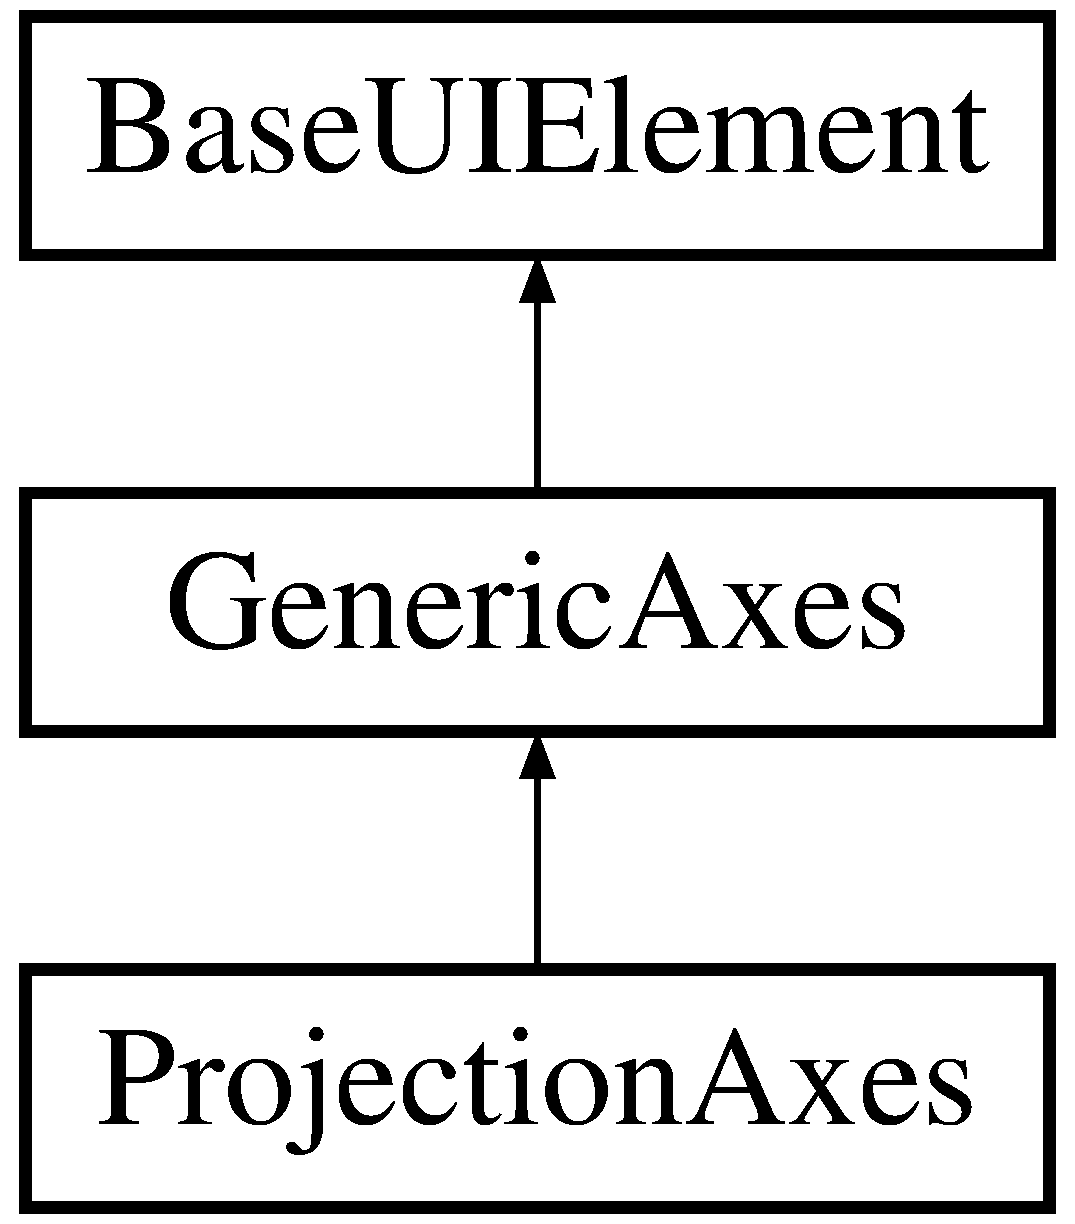
\includegraphics[height=3.000000cm]{classProjectionAxes}
\end{center}
\end{figure}
\subsection*{Public Member Functions}
\begin{DoxyCompactItemize}
\item 
\hypertarget{classProjectionAxes_acfda67974323b9c7d71cc5825e8aaa4d}{{\bfseries Projection\-Axes} (int x, int y, double w, double h, int t)}\label{classProjectionAxes_acfda67974323b9c7d71cc5825e8aaa4d}

\item 
\hypertarget{classProjectionAxes_ad5542f2256adb9c782d1a8025c2ace37}{void {\bfseries set\-Position} (int, int, int, int)}\label{classProjectionAxes_ad5542f2256adb9c782d1a8025c2ace37}

\item 
\hypertarget{classProjectionAxes_adaeb9de4f99cfc73d2d79ddeb2c867db}{void {\bfseries update\-Spike\-Data} (\hyperlink{structSpikeObject}{Spike\-Object} s)}\label{classProjectionAxes_adaeb9de4f99cfc73d2d79ddeb2c867db}

\item 
\hypertarget{classProjectionAxes_a8e1e5c29651418d405afa93880c24399}{void {\bfseries set\-Point\-Color} (G\-Lfloat r, G\-Lfloat g, G\-Lfloat b)}\label{classProjectionAxes_a8e1e5c29651418d405afa93880c24399}

\item 
\hypertarget{classProjectionAxes_ad3c22e6128ba905240b7b7e0b630faf5}{void {\bfseries set\-Grid\-Color} (G\-Lfloat, G\-Lfloat, G\-Lfloat)}\label{classProjectionAxes_ad3c22e6128ba905240b7b7e0b630faf5}

\item 
\hypertarget{classProjectionAxes_adae3c04c3a1847bee1105474380fff02}{void {\bfseries clear} ()}\label{classProjectionAxes_adae3c04c3a1847bee1105474380fff02}

\item 
\hypertarget{classProjectionAxes_a483416ad6a461383c148504857d96fce}{void {\bfseries invalidate\-Texture} ()}\label{classProjectionAxes_a483416ad6a461383c148504857d96fce}

\item 
\hypertarget{classProjectionAxes_a42d89f47f6bb4dee062a190d1fa54aa3}{void {\bfseries redraw} ()}\label{classProjectionAxes_a42d89f47f6bb4dee062a190d1fa54aa3}

\end{DoxyCompactItemize}
\subsection*{Public Attributes}
\begin{DoxyCompactItemize}
\item 
\hypertarget{classProjectionAxes_af7f323bed1ddf6b125cf45bf8852d4c8}{bool {\bfseries overlay}}\label{classProjectionAxes_af7f323bed1ddf6b125cf45bf8852d4c8}

\item 
\hypertarget{classProjectionAxes_a094fc5c16540419ca3ded31d378790e1}{bool {\bfseries draw\-Grid}}\label{classProjectionAxes_a094fc5c16540419ca3ded31d378790e1}

\item 
\hypertarget{classProjectionAxes_a0dc4634471d11274ffea606ff2263a28}{bool {\bfseries convert\-Label\-Units}}\label{classProjectionAxes_a0dc4634471d11274ffea606ff2263a28}

\end{DoxyCompactItemize}
\subsection*{Protected Member Functions}
\begin{DoxyCompactItemize}
\item 
\hypertarget{classProjectionAxes_aa16be5ea3376a6aa96b09a5a00d0388a}{void {\bfseries plot} ()}\label{classProjectionAxes_aa16be5ea3376a6aa96b09a5a00d0388a}

\end{DoxyCompactItemize}
\subsection*{Private Member Functions}
\begin{DoxyCompactItemize}
\item 
\hypertarget{classProjectionAxes_adf8c6ab7587cfd2f68bcd921c0deefd5}{void {\bfseries draw\-Projection\-Grid} (int thold, int gain)}\label{classProjectionAxes_adf8c6ab7587cfd2f68bcd921c0deefd5}

\item 
\hypertarget{classProjectionAxes_a79002692644c7b571edfafdcb3e2ed38}{void {\bfseries calc\-Waveform\-Peak\-Idx} (int, int, int $\ast$, int $\ast$)}\label{classProjectionAxes_a79002692644c7b571edfafdcb3e2ed38}

\item 
\hypertarget{classProjectionAxes_a46b514befc5d4cd1309e9a88fad72a3e}{void {\bfseries create\-Texture} ()}\label{classProjectionAxes_a46b514befc5d4cd1309e9a88fad72a3e}

\item 
\hypertarget{classProjectionAxes_a3e3a0956302f8b1e92ce542301e6c8e1}{void {\bfseries create\-F\-B\-O} ()}\label{classProjectionAxes_a3e3a0956302f8b1e92ce542301e6c8e1}

\item 
\hypertarget{classProjectionAxes_a26ae1675878b7db62b06fc97ae96b17e}{void {\bfseries draw\-Spikes\-To\-Texture} (bool all\-Spikes)}\label{classProjectionAxes_a26ae1675878b7db62b06fc97ae96b17e}

\item 
\hypertarget{classProjectionAxes_a662c5addb15eb47a381dab098128ddab}{void {\bfseries draw\-Textured\-Quad} ()}\label{classProjectionAxes_a662c5addb15eb47a381dab098128ddab}

\item 
\hypertarget{classProjectionAxes_a5d16f25291dce8fcac912d8759c9af1c}{void {\bfseries plot\-Old\-Spikes} (bool all\-Spikes)}\label{classProjectionAxes_a5d16f25291dce8fcac912d8759c9af1c}

\item 
\hypertarget{classProjectionAxes_a093baf0ba53ad3dd8b7bee92b3874665}{void {\bfseries plot\-Newest\-Spike} ()}\label{classProjectionAxes_a093baf0ba53ad3dd8b7bee92b3874665}

\item 
\hypertarget{classProjectionAxes_a2150462895139ddbf32632057e9c4df6}{void {\bfseries clear\-Texture} ()}\label{classProjectionAxes_a2150462895139ddbf32632057e9c4df6}

\item 
\hypertarget{classProjectionAxes_a5b3c3c7be28c6f82a403aeeab069272b}{void {\bfseries validate\-Texture} ()}\label{classProjectionAxes_a5b3c3c7be28c6f82a403aeeab069272b}

\end{DoxyCompactItemize}
\subsection*{Private Attributes}
\begin{DoxyCompactItemize}
\item 
\hypertarget{classProjectionAxes_a189c8dba7710b4b7939f69ee4972aa62}{G\-Lfloat {\bfseries point\-Color} \mbox{[}3\mbox{]}}\label{classProjectionAxes_a189c8dba7710b4b7939f69ee4972aa62}

\item 
\hypertarget{classProjectionAxes_aa416fc33e07f3784775f60d8d473414a}{G\-Lfloat {\bfseries grid\-Color} \mbox{[}3\mbox{]}}\label{classProjectionAxes_aa416fc33e07f3784775f60d8d473414a}

\item 
\hypertarget{classProjectionAxes_ae504a51a628ee4b473fbf63f1fce36e7}{int {\bfseries amp\-Buffer} \mbox{[}2\mbox{]}\mbox{[}A\-M\-P\-\_\-\-B\-U\-F\-F\-\_\-\-M\-A\-X\-\_\-\-S\-I\-Z\-E\mbox{]}}\label{classProjectionAxes_ae504a51a628ee4b473fbf63f1fce36e7}

\item 
\hypertarget{classProjectionAxes_a7fbced8c262d9c180629d2bac7c390b7}{uint16\-\_\-t {\bfseries buff\-Idx}}\label{classProjectionAxes_a7fbced8c262d9c180629d2bac7c390b7}

\item 
\hypertarget{classProjectionAxes_a467cfa2f128518849701846512989fda}{uint64\-\_\-t {\bfseries total\-Spikes}}\label{classProjectionAxes_a467cfa2f128518849701846512989fda}

\item 
\hypertarget{classProjectionAxes_af30eec2bec1ee2c4bf455f9af75a329e}{int {\bfseries amp\-Dim1}}\label{classProjectionAxes_af30eec2bec1ee2c4bf455f9af75a329e}

\item 
\hypertarget{classProjectionAxes_afee898e5030d22ccf8638dd838f45412}{int {\bfseries amp\-Dim2}}\label{classProjectionAxes_afee898e5030d22ccf8638dd838f45412}

\item 
\hypertarget{classProjectionAxes_acaeacee8aecad5416a06fbbd3526032a}{bool {\bfseries new\-Spike}}\label{classProjectionAxes_acaeacee8aecad5416a06fbbd3526032a}

\item 
\hypertarget{classProjectionAxes_ad36f7f83c3290d9d4f19e7d1a55bbd43}{G\-Luint {\bfseries fbo\-Id}}\label{classProjectionAxes_ad36f7f83c3290d9d4f19e7d1a55bbd43}

\item 
\hypertarget{classProjectionAxes_aaf12fb5eb0b3cc8f6f256bf42790b20f}{G\-Luint {\bfseries texture\-Id}}\label{classProjectionAxes_aaf12fb5eb0b3cc8f6f256bf42790b20f}

\item 
\hypertarget{classProjectionAxes_a33abda6700f7276e75b7f2f295b0299e}{G\-Luint {\bfseries rbo\-Id}}\label{classProjectionAxes_a33abda6700f7276e75b7f2f295b0299e}

\item 
\hypertarget{classProjectionAxes_a0515ac3013f3dd5463276d4dd29a84b3}{int {\bfseries tex\-Width}}\label{classProjectionAxes_a0515ac3013f3dd5463276d4dd29a84b3}

\item 
\hypertarget{classProjectionAxes_ad31011ca9963309e7001c5431a078892}{int {\bfseries tex\-Height}}\label{classProjectionAxes_ad31011ca9963309e7001c5431a078892}

\item 
\hypertarget{classProjectionAxes_a2bc0df7a19b189984f35a6a2b0e62140}{bool {\bfseries clear\-On\-Next\-Draw}}\label{classProjectionAxes_a2bc0df7a19b189984f35a6a2b0e62140}

\item 
\hypertarget{classProjectionAxes_a19f0f227afbf46f180484bcddba6f86e}{bool {\bfseries is\-Texture\-Valid}}\label{classProjectionAxes_a19f0f227afbf46f180484bcddba6f86e}

\item 
\hypertarget{classProjectionAxes_a0ad6b4ee29d3fee0279b432b98b7a115}{bool {\bfseries fbo\-Created}}\label{classProjectionAxes_a0ad6b4ee29d3fee0279b432b98b7a115}

\item 
\hypertarget{classProjectionAxes_a0a0b1a9ef33eaae6291c3bcab1ed36ea}{bool {\bfseries all\-Spikes\-Next\-Render}}\label{classProjectionAxes_a0a0b1a9ef33eaae6291c3bcab1ed36ea}

\end{DoxyCompactItemize}
\subsection*{Additional Inherited Members}


The documentation for this class was generated from the following file\-:\begin{DoxyCompactItemize}
\item 
Processors/\-Visualization/\-Spike\-Plotting/Projection\-Axes.\-h\end{DoxyCompactItemize}

\hypertarget{classRecordButton}{\section{Record\-Button Class Reference}
\label{classRecordButton}\index{Record\-Button@{Record\-Button}}
}


The documentation for this class was generated from the following file\-:\begin{DoxyCompactItemize}
\item 
U\-I/Control\-Panel.\-h\end{DoxyCompactItemize}

\hypertarget{classRecordNode}{\section{Record\-Node Class Reference}
\label{classRecordNode}\index{Record\-Node@{Record\-Node}}
}


{\ttfamily \#include $<$Record\-Node.\-h$>$}

Inheritance diagram for Record\-Node\-:\begin{figure}[H]
\begin{center}
\leavevmode
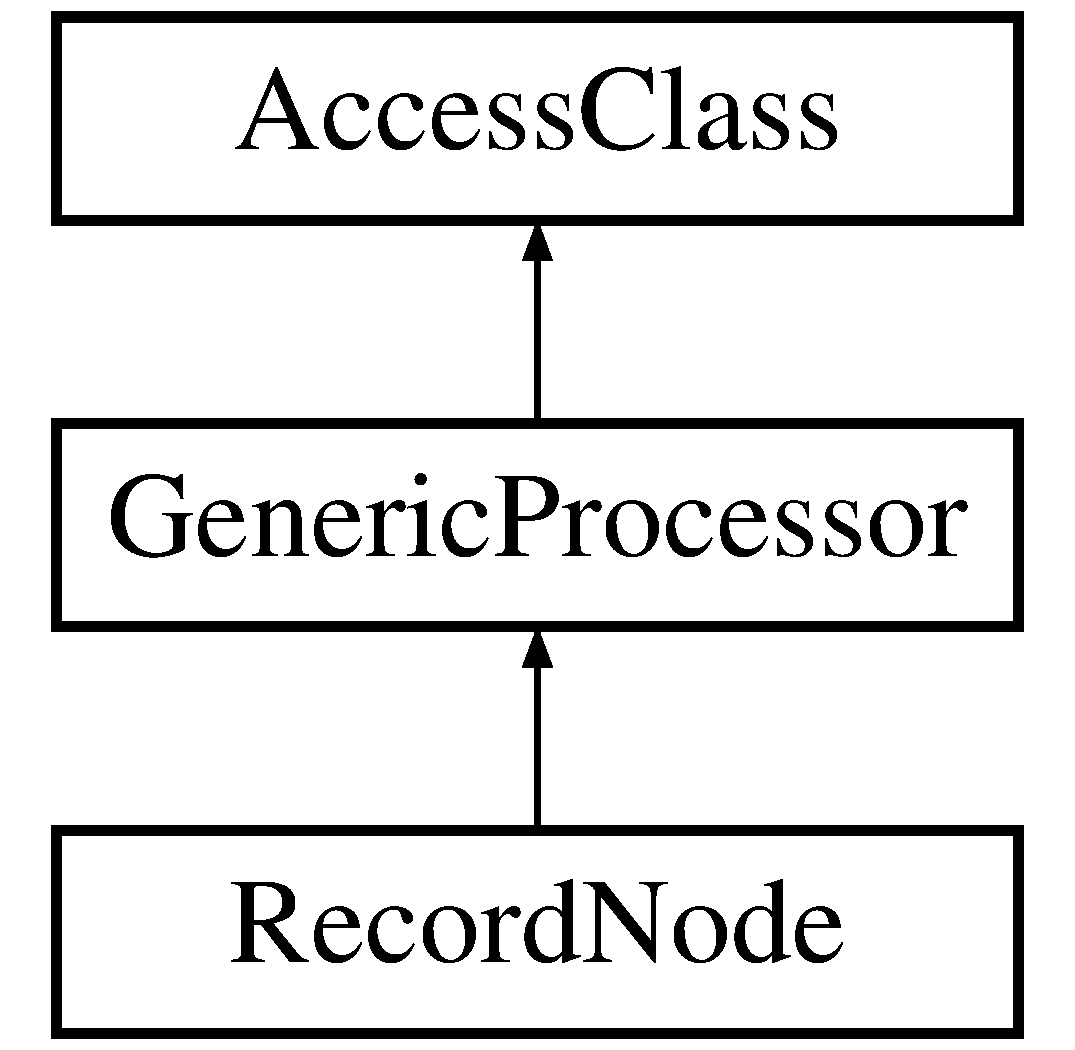
\includegraphics[height=3.000000cm]{classRecordNode}
\end{center}
\end{figure}
\subsection*{Classes}
\begin{DoxyCompactItemize}
\item 
struct \hyperlink{structRecordNode_1_1Channel}{Channel}
\end{DoxyCompactItemize}
\subsection*{Public Member Functions}
\begin{DoxyCompactItemize}
\item 
\hypertarget{classRecordNode_aca58ffeeeb9a112bfe4a8275d3e8e3ba}{void {\bfseries process} (Audio\-Sample\-Buffer \&buffer, Midi\-Buffer \&event\-Buffer, int \&n\-Samples)}\label{classRecordNode_aca58ffeeeb9a112bfe4a8275d3e8e3ba}

\item 
\hypertarget{classRecordNode_a8a63274afcbea876bb3d83b47ca40c2f}{void {\bfseries set\-Parameter} (int parameter\-Index, float new\-Value)}\label{classRecordNode_a8a63274afcbea876bb3d83b47ca40c2f}

\item 
\hypertarget{classRecordNode_a4047f96e619200aeaf00795e70c7cef6}{void {\bfseries add\-Input\-Channel} (\hyperlink{classGenericProcessor}{Generic\-Processor} $\ast$source\-Node, int chan)}\label{classRecordNode_a4047f96e619200aeaf00795e70c7cef6}

\item 
\hypertarget{classRecordNode_a9b4fa6a3b6662d9888184dd3ad013872}{bool {\bfseries enable} ()}\label{classRecordNode_a9b4fa6a3b6662d9888184dd3ad013872}

\item 
\hypertarget{classRecordNode_ae020d2f723fb1468f48f14d76d007202}{bool {\bfseries disable} ()}\label{classRecordNode_ae020d2f723fb1468f48f14d76d007202}

\item 
float \hyperlink{classRecordNode_a208709d4b0f959a845f10490acde9ca8}{get\-Free\-Space} ()
\item 
\hypertarget{classRecordNode_a7fd11ada72f04467e0dc8fc9a55fba42}{void {\bfseries set\-Channel} (int id, int chan)}\label{classRecordNode_a7fd11ada72f04467e0dc8fc9a55fba42}

\item 
\hypertarget{classRecordNode_afe6506668d8072656c54a843abde276d}{void {\bfseries set\-Channel\-Status} (int chan, bool status)}\label{classRecordNode_afe6506668d8072656c54a843abde276d}

\item 
\hypertarget{classRecordNode_aaa35ce70d9da415b021a426e8cd43765}{void {\bfseries reset\-Connections} ()}\label{classRecordNode_aaa35ce70d9da415b021a426e8cd43765}

\item 
\hypertarget{classRecordNode_a65b8be30adce613a4f4e0acf684b787c}{bool {\bfseries is\-Audio\-Or\-Record\-Node} ()}\label{classRecordNode_a65b8be30adce613a4f4e0acf684b787c}

\item 
\hypertarget{classRecordNode_a18e27b2842124012d915fdfd2e272d96}{void {\bfseries filename\-Component\-Changed} (Filename\-Component $\ast$)}\label{classRecordNode_a18e27b2842124012d915fdfd2e272d96}

\item 
\hypertarget{classRecordNode_abbbb21fd91cc96595d377addb3e71bf5}{void {\bfseries create\-New\-Directory} ()}\label{classRecordNode_abbbb21fd91cc96595d377addb3e71bf5}

\end{DoxyCompactItemize}
\subsection*{Private Member Functions}
\begin{DoxyCompactItemize}
\item 
\hypertarget{classRecordNode_ac0b7f68959e87a84b7c8dd2e31dce4cd}{void {\bfseries close\-All\-Files} ()}\label{classRecordNode_ac0b7f68959e87a84b7c8dd2e31dce4cd}

\item 
void \hyperlink{classRecordNode_a8ef29a4715a5034bf2e101ac9a06a1d7}{write\-Continuous\-Buffer} (float $\ast$data, int n\-Samples, int channel)
\item 
void \hyperlink{classRecordNode_ade1f1f1fdff335a3d67632368154b853}{write\-Event\-Buffer} (Midi\-Message \&event, int node, int channel)
\item 
\hypertarget{classRecordNode_adfd8695c0064f1306a66c9096e486375}{{\bfseries J\-U\-C\-E\-\_\-\-D\-E\-C\-L\-A\-R\-E\-\_\-\-N\-O\-N\-\_\-\-C\-O\-P\-Y\-A\-B\-L\-E\-\_\-\-W\-I\-T\-H\-\_\-\-L\-E\-A\-K\-\_\-\-D\-E\-T\-E\-C\-T\-O\-R} (\hyperlink{classRecordNode}{Record\-Node})}\label{classRecordNode_adfd8695c0064f1306a66c9096e486375}

\end{DoxyCompactItemize}
\subsection*{Private Attributes}
\begin{DoxyCompactItemize}
\item 
bool \hyperlink{classRecordNode_a70adffca8ea1721773c80ad6c4a844e1}{is\-Recording}
\item 
\hypertarget{classRecordNode_a872f0369bb5a3eb28b0368efecdd27d5}{bool {\bfseries is\-Processing}}\label{classRecordNode_a872f0369bb5a3eb28b0368efecdd27d5}

\item 
\hypertarget{classRecordNode_a35774cd75d42f08f8bdec2132d0529e3}{bool {\bfseries signal\-Files\-Should\-Close}}\label{classRecordNode_a35774cd75d42f08f8bdec2132d0529e3}

\item 
File \hyperlink{classRecordNode_a5109feb0a2d1821616f3ff8ba04ee8e1}{data\-Directory}
\item 
File \hyperlink{classRecordNode_a6b6bbb72fc226f1de138175d575e62e1}{root\-Folder}
\item 
bool \hyperlink{classRecordNode_abc8b3b93a3912fa0c0ed6438508a7c78}{new\-Data\-Folder}
\item 
int16 $\ast$ \hyperlink{classRecordNode_a01ef6a171ab8d2a81e5cbc54293ca4cc}{continuous\-Data\-Buffer}
\item 
int64 \hyperlink{classRecordNode_a154d4c809090e282cdd99098c0d701c9}{timestamp}
\item 
Time \hyperlink{classRecordNode_a406bc13e786db7c14f1cd8b183ebc0e0}{timer}
\item 
std\-::map$<$ int, \hyperlink{structRecordNode_1_1Channel}{Channel} $>$ \hyperlink{classRecordNode_a5a1f8fe9e3100ab74d4bb2650be91f6d}{continuous\-Channels}
\item 
std\-::map$<$ int, std\-::map$<$ int, \\*
\hyperlink{structRecordNode_1_1Channel}{Channel} $>$ $>$ \hyperlink{classRecordNode_a1abec1e7ff14c068315ba3d661339553}{event\-Channels}
\end{DoxyCompactItemize}
\subsection*{Additional Inherited Members}


\subsection{Detailed Description}
Receives inputs from all processors that want to save their data. Writes data to disk using fwrite.

Receives a signal from the \hyperlink{classControlPanel}{Control\-Panel} to begin recording.

\begin{DoxySeeAlso}{See also}
\hyperlink{classGenericProcessor}{Generic\-Processor}, \hyperlink{classControlPanel}{Control\-Panel} 
\end{DoxySeeAlso}


\subsection{Member Function Documentation}
\hypertarget{classRecordNode_a208709d4b0f959a845f10490acde9ca8}{\index{Record\-Node@{Record\-Node}!get\-Free\-Space@{get\-Free\-Space}}
\index{get\-Free\-Space@{get\-Free\-Space}!RecordNode@{Record\-Node}}
\subsubsection[{get\-Free\-Space}]{\setlength{\rightskip}{0pt plus 5cm}float Record\-Node\-::get\-Free\-Space (
\begin{DoxyParamCaption}
{}
\end{DoxyParamCaption}
)}}\label{classRecordNode_a208709d4b0f959a845f10490acde9ca8}
Called by the \hyperlink{classControlPanel}{Control\-Panel} to determine the amount of space left in the current data\-Directory. \hypertarget{classRecordNode_a8ef29a4715a5034bf2e101ac9a06a1d7}{\index{Record\-Node@{Record\-Node}!write\-Continuous\-Buffer@{write\-Continuous\-Buffer}}
\index{write\-Continuous\-Buffer@{write\-Continuous\-Buffer}!RecordNode@{Record\-Node}}
\subsubsection[{write\-Continuous\-Buffer}]{\setlength{\rightskip}{0pt plus 5cm}void Record\-Node\-::write\-Continuous\-Buffer (
\begin{DoxyParamCaption}
\item[{float $\ast$}]{data, }
\item[{int}]{n\-Samples, }
\item[{int}]{channel}
\end{DoxyParamCaption}
)\hspace{0.3cm}{\ttfamily [private]}}}\label{classRecordNode_a8ef29a4715a5034bf2e101ac9a06a1d7}
Method for writing continuous buffers to disk. \hypertarget{classRecordNode_ade1f1f1fdff335a3d67632368154b853}{\index{Record\-Node@{Record\-Node}!write\-Event\-Buffer@{write\-Event\-Buffer}}
\index{write\-Event\-Buffer@{write\-Event\-Buffer}!RecordNode@{Record\-Node}}
\subsubsection[{write\-Event\-Buffer}]{\setlength{\rightskip}{0pt plus 5cm}void Record\-Node\-::write\-Event\-Buffer (
\begin{DoxyParamCaption}
\item[{Midi\-Message \&}]{event, }
\item[{int}]{node, }
\item[{int}]{channel}
\end{DoxyParamCaption}
)\hspace{0.3cm}{\ttfamily [private]}}}\label{classRecordNode_ade1f1f1fdff335a3d67632368154b853}
Method for writing event buffers to disk. 

\subsection{Member Data Documentation}
\hypertarget{classRecordNode_a5a1f8fe9e3100ab74d4bb2650be91f6d}{\index{Record\-Node@{Record\-Node}!continuous\-Channels@{continuous\-Channels}}
\index{continuous\-Channels@{continuous\-Channels}!RecordNode@{Record\-Node}}
\subsubsection[{continuous\-Channels}]{\setlength{\rightskip}{0pt plus 5cm}std\-::map$<$int, {\bf Channel}$>$ Record\-Node\-::continuous\-Channels\hspace{0.3cm}{\ttfamily [private]}}}\label{classRecordNode_a5a1f8fe9e3100ab74d4bb2650be91f6d}
Map of continuous channels. \hypertarget{classRecordNode_a01ef6a171ab8d2a81e5cbc54293ca4cc}{\index{Record\-Node@{Record\-Node}!continuous\-Data\-Buffer@{continuous\-Data\-Buffer}}
\index{continuous\-Data\-Buffer@{continuous\-Data\-Buffer}!RecordNode@{Record\-Node}}
\subsubsection[{continuous\-Data\-Buffer}]{\setlength{\rightskip}{0pt plus 5cm}int16$\ast$ Record\-Node\-::continuous\-Data\-Buffer\hspace{0.3cm}{\ttfamily [private]}}}\label{classRecordNode_a01ef6a171ab8d2a81e5cbc54293ca4cc}
Holds data that has been converted from float to int16 before saving. \hypertarget{classRecordNode_a5109feb0a2d1821616f3ff8ba04ee8e1}{\index{Record\-Node@{Record\-Node}!data\-Directory@{data\-Directory}}
\index{data\-Directory@{data\-Directory}!RecordNode@{Record\-Node}}
\subsubsection[{data\-Directory}]{\setlength{\rightskip}{0pt plus 5cm}File Record\-Node\-::data\-Directory\hspace{0.3cm}{\ttfamily [private]}}}\label{classRecordNode_a5109feb0a2d1821616f3ff8ba04ee8e1}
User-\/selectable directory for saving data files. Currently defaults to the user's home directory. \hypertarget{classRecordNode_a1abec1e7ff14c068315ba3d661339553}{\index{Record\-Node@{Record\-Node}!event\-Channels@{event\-Channels}}
\index{event\-Channels@{event\-Channels}!RecordNode@{Record\-Node}}
\subsubsection[{event\-Channels}]{\setlength{\rightskip}{0pt plus 5cm}std\-::map$<$int, std\-::map$<$int,{\bf Channel}$>$ $>$ Record\-Node\-::event\-Channels\hspace{0.3cm}{\ttfamily [private]}}}\label{classRecordNode_a1abec1e7ff14c068315ba3d661339553}
Map of event channels. \hypertarget{classRecordNode_a70adffca8ea1721773c80ad6c4a844e1}{\index{Record\-Node@{Record\-Node}!is\-Recording@{is\-Recording}}
\index{is\-Recording@{is\-Recording}!RecordNode@{Record\-Node}}
\subsubsection[{is\-Recording}]{\setlength{\rightskip}{0pt plus 5cm}bool Record\-Node\-::is\-Recording\hspace{0.3cm}{\ttfamily [private]}}}\label{classRecordNode_a70adffca8ea1721773c80ad6c4a844e1}
Keep the \hyperlink{classRecordNode}{Record\-Node} informed of acquisition and record states. \hypertarget{classRecordNode_abc8b3b93a3912fa0c0ed6438508a7c78}{\index{Record\-Node@{Record\-Node}!new\-Data\-Folder@{new\-Data\-Folder}}
\index{new\-Data\-Folder@{new\-Data\-Folder}!RecordNode@{Record\-Node}}
\subsubsection[{new\-Data\-Folder}]{\setlength{\rightskip}{0pt plus 5cm}bool Record\-Node\-::new\-Data\-Folder\hspace{0.3cm}{\ttfamily [private]}}}\label{classRecordNode_abc8b3b93a3912fa0c0ed6438508a7c78}
Determines whether a new root\-Folder is created when recording begins. \hypertarget{classRecordNode_a6b6bbb72fc226f1de138175d575e62e1}{\index{Record\-Node@{Record\-Node}!root\-Folder@{root\-Folder}}
\index{root\-Folder@{root\-Folder}!RecordNode@{Record\-Node}}
\subsubsection[{root\-Folder}]{\setlength{\rightskip}{0pt plus 5cm}File Record\-Node\-::root\-Folder\hspace{0.3cm}{\ttfamily [private]}}}\label{classRecordNode_a6b6bbb72fc226f1de138175d575e62e1}
Automatically generated folder for each recording session. \hypertarget{classRecordNode_a406bc13e786db7c14f1cd8b183ebc0e0}{\index{Record\-Node@{Record\-Node}!timer@{timer}}
\index{timer@{timer}!RecordNode@{Record\-Node}}
\subsubsection[{timer}]{\setlength{\rightskip}{0pt plus 5cm}Time Record\-Node\-::timer\hspace{0.3cm}{\ttfamily [private]}}}\label{classRecordNode_a406bc13e786db7c14f1cd8b183ebc0e0}
Used to generate timestamps if none are given. \hypertarget{classRecordNode_a154d4c809090e282cdd99098c0d701c9}{\index{Record\-Node@{Record\-Node}!timestamp@{timestamp}}
\index{timestamp@{timestamp}!RecordNode@{Record\-Node}}
\subsubsection[{timestamp}]{\setlength{\rightskip}{0pt plus 5cm}int64 Record\-Node\-::timestamp\hspace{0.3cm}{\ttfamily [private]}}}\label{classRecordNode_a154d4c809090e282cdd99098c0d701c9}
Integer timestamp saved for each buffer. 

The documentation for this class was generated from the following file\-:\begin{DoxyCompactItemize}
\item 
Processors/Record\-Node.\-h\end{DoxyCompactItemize}

\hypertarget{classResamplingNode}{\section{Resampling\-Node Class Reference}
\label{classResamplingNode}\index{Resampling\-Node@{Resampling\-Node}}
}


{\ttfamily \#include $<$Resampling\-Node.\-h$>$}

Inheritance diagram for Resampling\-Node\-:\begin{figure}[H]
\begin{center}
\leavevmode
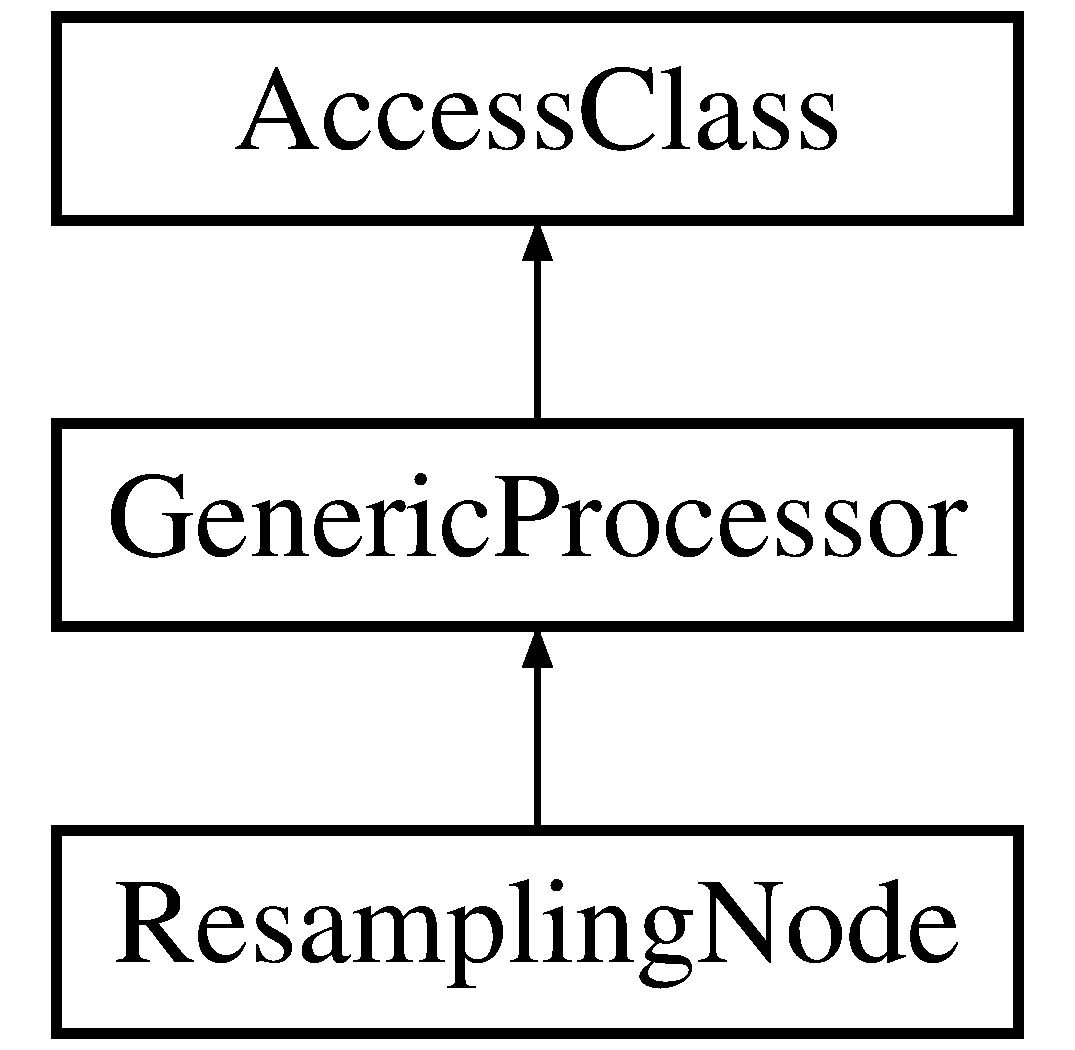
\includegraphics[height=3.000000cm]{classResamplingNode}
\end{center}
\end{figure}
\subsection*{Public Member Functions}
\begin{DoxyCompactItemize}
\item 
\hypertarget{classResamplingNode_acd5711ddad27cdd6155e53b180d5b387}{{\bfseries Resampling\-Node} (bool dest\-Buffer\-Is\-Temp\-Buffer)}\label{classResamplingNode_acd5711ddad27cdd6155e53b180d5b387}

\item 
\hypertarget{classResamplingNode_a02443ca9ed779e974ff222cfa0d4bbdd}{Audio\-Sample\-Buffer $\ast$ {\bfseries get\-Buffer\-Address} ()}\label{classResamplingNode_a02443ca9ed779e974ff222cfa0d4bbdd}

\item 
\hypertarget{classResamplingNode_afe65c4c590a9d2839982e3d9c1dbdbca}{void {\bfseries update\-Filter} ()}\label{classResamplingNode_afe65c4c590a9d2839982e3d9c1dbdbca}

\item 
\hypertarget{classResamplingNode_ad20396badb3000d315392d059846c803}{void {\bfseries prepare\-To\-Play} (double sample\-Rate, int estimated\-Samples\-Per\-Block)}\label{classResamplingNode_ad20396badb3000d315392d059846c803}

\item 
\hypertarget{classResamplingNode_af1298a6340299392d6e5503a29dca423}{void {\bfseries release\-Resources} ()}\label{classResamplingNode_af1298a6340299392d6e5503a29dca423}

\item 
\hypertarget{classResamplingNode_aad4c79707b095fa925c33ccaa208b576}{void {\bfseries process} (Audio\-Sample\-Buffer \&buffer, Midi\-Buffer \&midi\-Messages, int \&n\-Samples)}\label{classResamplingNode_aad4c79707b095fa925c33ccaa208b576}

\item 
\hypertarget{classResamplingNode_a52b642ff6993476725a1f38bfde2abff}{void {\bfseries set\-Parameter} (int parameter\-Index, float new\-Value)}\label{classResamplingNode_a52b642ff6993476725a1f38bfde2abff}

\item 
\hypertarget{classResamplingNode_a897e78c484e825a5809033d241a41d63}{Audio\-Sample\-Buffer $\ast$ {\bfseries get\-Continuous\-Buffer} ()}\label{classResamplingNode_a897e78c484e825a5809033d241a41d63}

\end{DoxyCompactItemize}
\subsection*{Private Member Functions}
\begin{DoxyCompactItemize}
\item 
\hypertarget{classResamplingNode_a83436544ad2834b542f804dd5885373f}{void {\bfseries write\-Continuous\-Buffer} (float $\ast$, int, int)}\label{classResamplingNode_a83436544ad2834b542f804dd5885373f}

\item 
\hypertarget{classResamplingNode_a26703f2abf9ffc9cf6a878118e3445cf}{{\bfseries J\-U\-C\-E\-\_\-\-D\-E\-C\-L\-A\-R\-E\-\_\-\-N\-O\-N\-\_\-\-C\-O\-P\-Y\-A\-B\-L\-E\-\_\-\-W\-I\-T\-H\-\_\-\-L\-E\-A\-K\-\_\-\-D\-E\-T\-E\-C\-T\-O\-R} (\hyperlink{classResamplingNode}{Resampling\-Node})}\label{classResamplingNode_a26703f2abf9ffc9cf6a878118e3445cf}

\end{DoxyCompactItemize}
\subsection*{Private Attributes}
\begin{DoxyCompactItemize}
\item 
\hypertarget{classResamplingNode_aa7f05e66d2921ccbacf1cabcca4a4651}{double {\bfseries source\-Buffer\-Sample\-Rate}}\label{classResamplingNode_aa7f05e66d2921ccbacf1cabcca4a4651}

\item 
\hypertarget{classResamplingNode_a67cd9e26669a6bf8106d3c04d139ddb3}{double {\bfseries dest\-Buffer\-Sample\-Rate}}\label{classResamplingNode_a67cd9e26669a6bf8106d3c04d139ddb3}

\item 
\hypertarget{classResamplingNode_a5fa83e04825b666f7d235daa51d7e957}{double {\bfseries ratio}}\label{classResamplingNode_a5fa83e04825b666f7d235daa51d7e957}

\item 
\hypertarget{classResamplingNode_a913ecb94e7f645956509b4596fb5bb48}{double {\bfseries last\-Ratio}}\label{classResamplingNode_a913ecb94e7f645956509b4596fb5bb48}

\item 
\hypertarget{classResamplingNode_a636ee58c8031d2dc4f54d39e22733cbe}{double {\bfseries dest\-Buffer\-Timebase\-Secs}}\label{classResamplingNode_a636ee58c8031d2dc4f54d39e22733cbe}

\item 
\hypertarget{classResamplingNode_aba52166a272e55c3ecac9b04def5f9f9}{int {\bfseries dest\-Buffer\-Width}}\label{classResamplingNode_aba52166a272e55c3ecac9b04def5f9f9}

\item 
\hypertarget{classResamplingNode_a277d1f3135f2990a337db2361ea0136d}{Dsp\-::\-Filter $\ast$ {\bfseries filter}}\label{classResamplingNode_a277d1f3135f2990a337db2361ea0136d}

\item 
\hypertarget{classResamplingNode_a6f839a4ec227047b673b7fd3693e4a37}{Audio\-Sample\-Buffer $\ast$ {\bfseries dest\-Buffer}}\label{classResamplingNode_a6f839a4ec227047b673b7fd3693e4a37}

\item 
\hypertarget{classResamplingNode_ac3c65285bdbbe5f9d939322345bdce9c}{Audio\-Sample\-Buffer $\ast$ {\bfseries temp\-Buffer}}\label{classResamplingNode_ac3c65285bdbbe5f9d939322345bdce9c}

\item 
\hypertarget{classResamplingNode_ae4abec313401261b728017a8906b30ad}{bool {\bfseries dest\-Buffer\-Is\-Temp\-Buffer}}\label{classResamplingNode_ae4abec313401261b728017a8906b30ad}

\item 
\hypertarget{classResamplingNode_a2b59f3115c928b57d13d07278a529557}{bool {\bfseries is\-Transmitting}}\label{classResamplingNode_a2b59f3115c928b57d13d07278a529557}

\item 
\hypertarget{classResamplingNode_ad1e104d2967a8192cf32c0100d0a9973}{int {\bfseries dest\-Buffer\-Pos}}\label{classResamplingNode_ad1e104d2967a8192cf32c0100d0a9973}

\item 
\hypertarget{classResamplingNode_a826f8f43016e44c1ef9d1de590f2fa87}{F\-I\-L\-E $\ast$ {\bfseries file}}\label{classResamplingNode_a826f8f43016e44c1ef9d1de590f2fa87}

\item 
\hypertarget{classResamplingNode_a639bf4cd47488ab90226f396a90a7620}{int64 {\bfseries timestamp}}\label{classResamplingNode_a639bf4cd47488ab90226f396a90a7620}

\item 
\hypertarget{classResamplingNode_a5d37e35ee5f83c4d9a2c3d582071f72c}{Time {\bfseries timer}}\label{classResamplingNode_a5d37e35ee5f83c4d9a2c3d582071f72c}

\item 
\hypertarget{classResamplingNode_abfc9d5a8d0cbfa093fbb35a8e24d574c}{int16 $\ast$ {\bfseries continuous\-Data\-Buffer}}\label{classResamplingNode_abfc9d5a8d0cbfa093fbb35a8e24d574c}

\end{DoxyCompactItemize}
\subsection*{Additional Inherited Members}


\subsection{Detailed Description}
--U\-N\-D\-E\-R C\-O\-N\-S\-T\-R\-U\-C\-T\-I\-O\-N--

Changes the sample rate of continuous data.

Code is based on Juce's Resampling\-Audio\-Source class.

\begin{DoxySeeAlso}{See also}
\hyperlink{classGenericProcessor}{Generic\-Processor} 
\end{DoxySeeAlso}


The documentation for this class was generated from the following file\-:\begin{DoxyCompactItemize}
\item 
Processors/Resampling\-Node.\-h\end{DoxyCompactItemize}

\hypertarget{classSelectorButton}{\section{Selector\-Button Class Reference}
\label{classSelectorButton}\index{Selector\-Button@{Selector\-Button}}
}
\subsection*{Public Member Functions}
\begin{DoxyCompactItemize}
\item 
\hypertarget{classSelectorButton_af8deaf4c36313d154158c13ee7456a54}{{\bfseries Selector\-Button} (const String \&name)}\label{classSelectorButton_af8deaf4c36313d154158c13ee7456a54}

\end{DoxyCompactItemize}
\subsection*{Private Member Functions}
\begin{DoxyCompactItemize}
\item 
\hypertarget{classSelectorButton_aba5280fae570ab8f06c46b758967f470}{void {\bfseries paint\-Button} (Graphics \&g, bool is\-Mouse\-Over, bool is\-Button\-Down)}\label{classSelectorButton_aba5280fae570ab8f06c46b758967f470}

\end{DoxyCompactItemize}


The documentation for this class was generated from the following file\-:\begin{DoxyCompactItemize}
\item 
Processors/\-Editors/Visualizer\-Editor.\-h\end{DoxyCompactItemize}

\hypertarget{classSignalChainManager}{\section{Signal\-Chain\-Manager Class Reference}
\label{classSignalChainManager}\index{Signal\-Chain\-Manager@{Signal\-Chain\-Manager}}
}
Inheritance diagram for Signal\-Chain\-Manager\-:\begin{figure}[H]
\begin{center}
\leavevmode
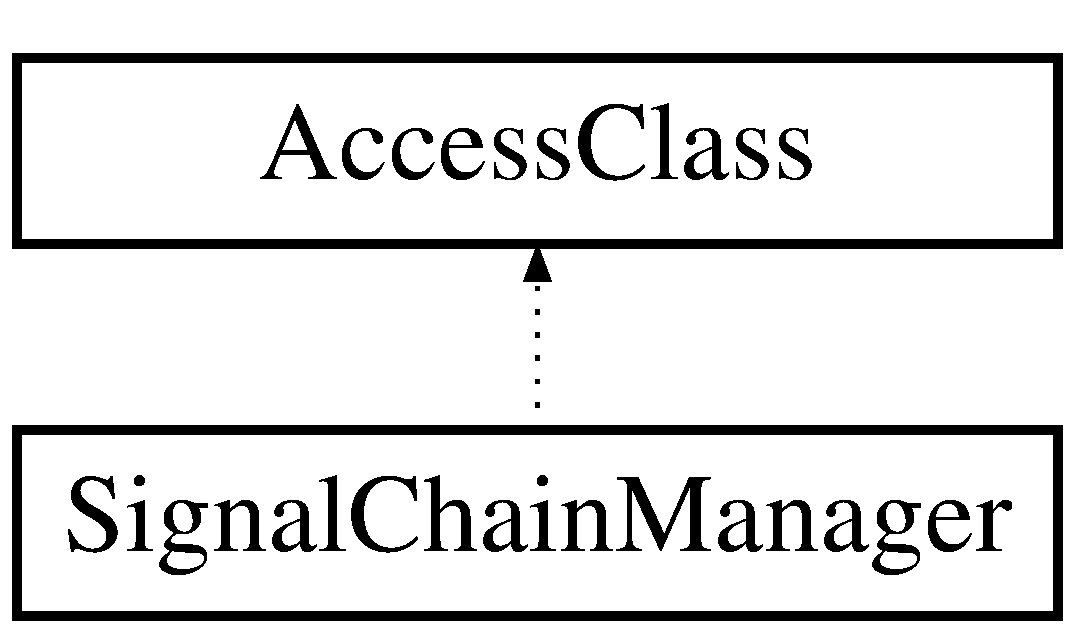
\includegraphics[height=2.000000cm]{classSignalChainManager}
\end{center}
\end{figure}
\subsection*{Public Member Functions}
\begin{DoxyCompactItemize}
\item 
\hypertarget{classSignalChainManager_a4c9c6d8e9d696ccd5a4abc92be3ffd53}{{\bfseries Signal\-Chain\-Manager} (\hyperlink{classEditorViewport}{Editor\-Viewport} $\ast$, Array$<$ \hyperlink{classGenericEditor}{Generic\-Editor} $\ast$, Critical\-Section $>$ \&, Array$<$ \hyperlink{classSignalChainTabButton}{Signal\-Chain\-Tab\-Button} $\ast$, Critical\-Section $>$ \&)}\label{classSignalChainManager_a4c9c6d8e9d696ccd5a4abc92be3ffd53}

\item 
\hypertarget{classSignalChainManager_a5810903aa311504a5f645ab8e3407621}{void {\bfseries update\-Visible\-Editors} (\hyperlink{classGenericEditor}{Generic\-Editor} $\ast$active\-Editor, int index, int insertion\-Point, int action)}\label{classSignalChainManager_a5810903aa311504a5f645ab8e3407621}

\item 
\hypertarget{classSignalChainManager_ac41a67727bc44712f423037cab412c93}{void {\bfseries create\-New\-Tab} (\hyperlink{classGenericEditor}{Generic\-Editor} $\ast$editor)}\label{classSignalChainManager_ac41a67727bc44712f423037cab412c93}

\item 
\hypertarget{classSignalChainManager_af82c227f0c963a6520a50c2556380a27}{void {\bfseries remove\-Tab} (int tab\-Index)}\label{classSignalChainManager_af82c227f0c963a6520a50c2556380a27}

\item 
\hypertarget{classSignalChainManager_a81fbdd194556d6c45024aaa4078e10a4}{void {\bfseries scroll\-Up} ()}\label{classSignalChainManager_a81fbdd194556d6c45024aaa4078e10a4}

\item 
\hypertarget{classSignalChainManager_a8d764a6707907ac99ffb22dd01286452}{void {\bfseries scroll\-Down} ()}\label{classSignalChainManager_a8d764a6707907ac99ffb22dd01286452}

\item 
\hypertarget{classSignalChainManager_a4653928f580543c4b9f8e995a6c50007}{void {\bfseries clear\-Signal\-Chain} ()}\label{classSignalChainManager_a4653928f580543c4b9f8e995a6c50007}

\end{DoxyCompactItemize}
\subsection*{Private Member Functions}
\begin{DoxyCompactItemize}
\item 
\hypertarget{classSignalChainManager_aae0be248f1f164de97d0321b95ca178a}{void {\bfseries refresh\-Tabs} ()}\label{classSignalChainManager_aae0be248f1f164de97d0321b95ca178a}

\end{DoxyCompactItemize}
\subsection*{Private Attributes}
\begin{DoxyCompactItemize}
\item 
\hypertarget{classSignalChainManager_ae2f623b0fb1f993e3b4993b87e839cce}{Array$<$ \hyperlink{classGenericEditor}{Generic\-Editor} \\*
$\ast$, Critical\-Section $>$ \& {\bfseries editor\-Array}}\label{classSignalChainManager_ae2f623b0fb1f993e3b4993b87e839cce}

\item 
\hypertarget{classSignalChainManager_a4cc0d862c46f508d5356a9ca150f3f16}{Array$<$ \hyperlink{classSignalChainTabButton}{Signal\-Chain\-Tab\-Button} \\*
$\ast$, Critical\-Section $>$ \& {\bfseries signal\-Chain\-Array}}\label{classSignalChainManager_a4cc0d862c46f508d5356a9ca150f3f16}

\item 
\hypertarget{classSignalChainManager_a61a72c10d356875f03212d48d5113e60}{\hyperlink{classEditorViewport}{Editor\-Viewport} $\ast$ {\bfseries ev}}\label{classSignalChainManager_a61a72c10d356875f03212d48d5113e60}

\item 
\hypertarget{classSignalChainManager_af2c3387af7ed6cda42c554681ed77eca}{int {\bfseries top\-Tab}}\label{classSignalChainManager_af2c3387af7ed6cda42c554681ed77eca}

\item 
\hypertarget{classSignalChainManager_aaf954c0fdb7e8fdf9092cdd9c3d4f7a4}{const int {\bfseries tab\-Size}}\label{classSignalChainManager_aaf954c0fdb7e8fdf9092cdd9c3d4f7a4}

\end{DoxyCompactItemize}


The documentation for this class was generated from the following file\-:\begin{DoxyCompactItemize}
\item 
U\-I/Signal\-Chain\-Manager.\-h\end{DoxyCompactItemize}

\hypertarget{classSignalChainScrollButton}{\section{Signal\-Chain\-Scroll\-Button Class Reference}
\label{classSignalChainScrollButton}\index{Signal\-Chain\-Scroll\-Button@{Signal\-Chain\-Scroll\-Button}}
}
\subsection*{Public Types}
\begin{DoxyCompactItemize}
\item 
enum {\bfseries type} \{ {\bfseries U\-P}, 
{\bfseries D\-O\-W\-N}
 \}
\end{DoxyCompactItemize}
\subsection*{Public Member Functions}
\begin{DoxyCompactItemize}
\item 
\hypertarget{classSignalChainScrollButton_a5fddb0fbc5fd4a2fead7884a06852207}{{\bfseries Signal\-Chain\-Scroll\-Button} (int type)}\label{classSignalChainScrollButton_a5fddb0fbc5fd4a2fead7884a06852207}

\item 
\hypertarget{classSignalChainScrollButton_a5e7091c485f0dee550c8b881d016edd6}{void {\bfseries set\-Active} (bool)}\label{classSignalChainScrollButton_a5e7091c485f0dee550c8b881d016edd6}

\end{DoxyCompactItemize}
\subsection*{Public Attributes}
\begin{DoxyCompactItemize}
\item 
\hypertarget{classSignalChainScrollButton_a5f9a528838cea1709e984c5937d11e1d}{bool {\bfseries is\-Active}}\label{classSignalChainScrollButton_a5f9a528838cea1709e984c5937d11e1d}

\item 
\hypertarget{classSignalChainScrollButton_a85745c7a19685327478de02182277c4c}{int {\bfseries direction}}\label{classSignalChainScrollButton_a85745c7a19685327478de02182277c4c}

\item 
\hypertarget{classSignalChainScrollButton_ad58deaed9ccbd226a3f267ec9b65fc35}{Drawable\-Path {\bfseries inactive}}\label{classSignalChainScrollButton_ad58deaed9ccbd226a3f267ec9b65fc35}

\item 
\hypertarget{classSignalChainScrollButton_a29548e0209d31b560c5d2d1b175f81fe}{Drawable\-Path {\bfseries active\-Normal}}\label{classSignalChainScrollButton_a29548e0209d31b560c5d2d1b175f81fe}

\item 
\hypertarget{classSignalChainScrollButton_a56bc06f2905a748dbe3318ba02e95148}{Drawable\-Path {\bfseries active\-Over}}\label{classSignalChainScrollButton_a56bc06f2905a748dbe3318ba02e95148}

\item 
\hypertarget{classSignalChainScrollButton_a6f33a146e8e19e8accf5ede376eb7010}{Drawable\-Path {\bfseries active\-Down}}\label{classSignalChainScrollButton_a6f33a146e8e19e8accf5ede376eb7010}

\end{DoxyCompactItemize}


The documentation for this class was generated from the following file\-:\begin{DoxyCompactItemize}
\item 
U\-I/Editor\-Viewport\-Buttons.\-h\end{DoxyCompactItemize}

\hypertarget{classSignalChainTabButton}{\section{Signal\-Chain\-Tab\-Button Class Reference}
\label{classSignalChainTabButton}\index{Signal\-Chain\-Tab\-Button@{Signal\-Chain\-Tab\-Button}}
}
\subsection*{Public Member Functions}
\begin{DoxyCompactItemize}
\item 
\hypertarget{classSignalChainTabButton_a1cf991048d95a2d4f61b337b00fc998c}{void {\bfseries set\-Editor} (\hyperlink{classGenericEditor}{Generic\-Editor} $\ast$p)}\label{classSignalChainTabButton_a1cf991048d95a2d4f61b337b00fc998c}

\item 
\hypertarget{classSignalChainTabButton_af1a7b2e2ad12fb97ef23faf0546c65e9}{void {\bfseries set\-Manager} (\hyperlink{classSignalChainManager}{Signal\-Chain\-Manager} $\ast$scm\-\_\-)}\label{classSignalChainTabButton_af1a7b2e2ad12fb97ef23faf0546c65e9}

\item 
\hypertarget{classSignalChainTabButton_a4fa278c7907b1f0d0b2284fc0e2c278e}{\hyperlink{classGenericEditor}{Generic\-Editor} $\ast$ {\bfseries get\-Editor} ()}\label{classSignalChainTabButton_a4fa278c7907b1f0d0b2284fc0e2c278e}

\item 
\hypertarget{classSignalChainTabButton_a6eea9cfbb95c76436324c8863121e6b5}{void {\bfseries set\-Number} (int n)}\label{classSignalChainTabButton_a6eea9cfbb95c76436324c8863121e6b5}

\item 
\hypertarget{classSignalChainTabButton_a79640058185f7d202bc2b8ef001cdcb3}{bool {\bfseries has\-New\-Connections} ()}\label{classSignalChainTabButton_a79640058185f7d202bc2b8ef001cdcb3}

\item 
\hypertarget{classSignalChainTabButton_a72c57cd3c717b6f9e60e85f6f303f275}{void {\bfseries has\-New\-Connections} (bool t)}\label{classSignalChainTabButton_a72c57cd3c717b6f9e60e85f6f303f275}

\end{DoxyCompactItemize}
\subsection*{Public Attributes}
\begin{DoxyCompactItemize}
\item 
\hypertarget{classSignalChainTabButton_aa496c1fd1cff3b6c3026166443053b83}{int {\bfseries offset}}\label{classSignalChainTabButton_aa496c1fd1cff3b6c3026166443053b83}

\end{DoxyCompactItemize}
\subsection*{Private Types}
\begin{DoxyCompactItemize}
\item 
enum {\bfseries actions} \{ {\bfseries A\-D\-D}, 
{\bfseries M\-O\-V\-E}, 
{\bfseries R\-E\-M\-O\-V\-E}, 
{\bfseries A\-C\-T\-I\-V\-A\-T\-E}
 \}
\end{DoxyCompactItemize}
\subsection*{Private Member Functions}
\begin{DoxyCompactItemize}
\item 
\hypertarget{classSignalChainTabButton_a22ce515c7e6f5593e9b8becea7bf2228}{void {\bfseries paint\-Button} (Graphics \&g, bool is\-Mouse\-Over, bool is\-Button\-Down)}\label{classSignalChainTabButton_a22ce515c7e6f5593e9b8becea7bf2228}

\item 
\hypertarget{classSignalChainTabButton_a7f4d77fb33b45457bae9b5f7e09d04e7}{void {\bfseries clicked} ()}\label{classSignalChainTabButton_a7f4d77fb33b45457bae9b5f7e09d04e7}

\end{DoxyCompactItemize}
\subsection*{Private Attributes}
\begin{DoxyCompactItemize}
\item 
\hypertarget{classSignalChainTabButton_afc50b5a3bd5a04c9a6551f8cbb8c017e}{\hyperlink{classGenericEditor}{Generic\-Editor} $\ast$ {\bfseries first\-Editor}}\label{classSignalChainTabButton_afc50b5a3bd5a04c9a6551f8cbb8c017e}

\item 
\hypertarget{classSignalChainTabButton_ae06686616b8f68e3194e3f6e7d9a134d}{\hyperlink{classSignalChainManager}{Signal\-Chain\-Manager} $\ast$ {\bfseries scm}}\label{classSignalChainTabButton_ae06686616b8f68e3194e3f6e7d9a134d}

\item 
\hypertarget{classSignalChainTabButton_aaf93a820d48a088fce328e71831c88b8}{int {\bfseries num}}\label{classSignalChainTabButton_aaf93a820d48a088fce328e71831c88b8}

\item 
\hypertarget{classSignalChainTabButton_a183bb733239fb3179fe00aecdc1c555f}{bool {\bfseries configuration\-Changed}}\label{classSignalChainTabButton_a183bb733239fb3179fe00aecdc1c555f}

\item 
\hypertarget{classSignalChainTabButton_a4ea8ef80ddbcdfa60a869a20f6136080}{Font {\bfseries button\-Font}}\label{classSignalChainTabButton_a4ea8ef80ddbcdfa60a869a20f6136080}

\end{DoxyCompactItemize}


The documentation for this class was generated from the following file\-:\begin{DoxyCompactItemize}
\item 
U\-I/Editor\-Viewport.\-h\end{DoxyCompactItemize}

\hypertarget{classSignalGenerator}{\section{Signal\-Generator Class Reference}
\label{classSignalGenerator}\index{Signal\-Generator@{Signal\-Generator}}
}


{\ttfamily \#include $<$Signal\-Generator.\-h$>$}

Inheritance diagram for Signal\-Generator\-:\begin{figure}[H]
\begin{center}
\leavevmode
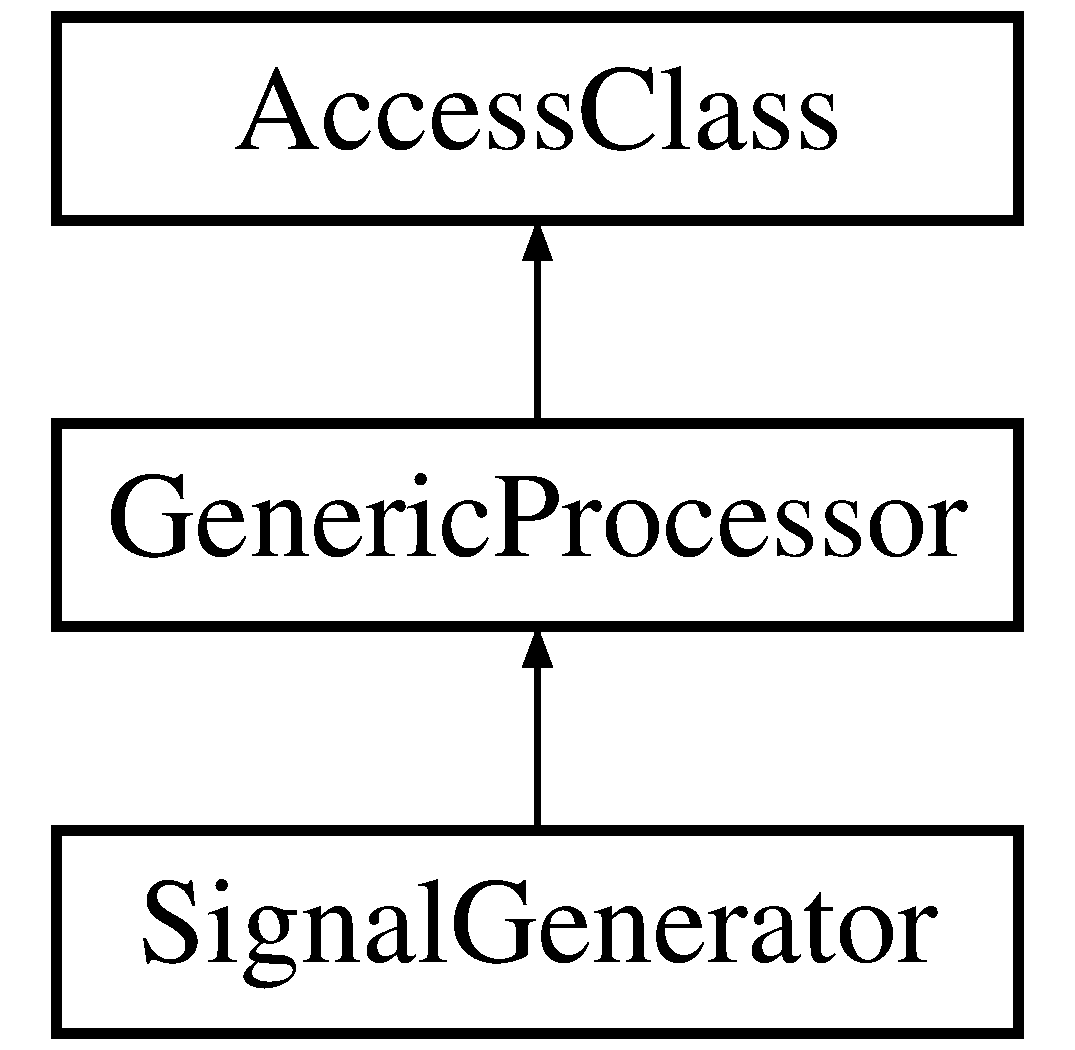
\includegraphics[height=3.000000cm]{classSignalGenerator}
\end{center}
\end{figure}
\subsection*{Public Member Functions}
\begin{DoxyCompactItemize}
\item 
\hypertarget{classSignalGenerator_a86bf3bfff12cee52e76031bad0e6d7be}{void {\bfseries process} (Audio\-Sample\-Buffer \&buffer, Midi\-Buffer \&midi\-Messages, int \&n\-Samples)}\label{classSignalGenerator_a86bf3bfff12cee52e76031bad0e6d7be}

\item 
\hypertarget{classSignalGenerator_a988310f92a5493a81084bc674a16fa7b}{void {\bfseries set\-Parameter} (int parameter\-Index, float new\-Value)}\label{classSignalGenerator_a988310f92a5493a81084bc674a16fa7b}

\item 
\hypertarget{classSignalGenerator_aa1eaf3cbb3f0ba0cfd30a3bfb1640680}{float {\bfseries get\-Sample\-Rate} ()}\label{classSignalGenerator_aa1eaf3cbb3f0ba0cfd30a3bfb1640680}

\item 
\hypertarget{classSignalGenerator_a91924c5fb098363a4c8f4fd8270d5606}{Audio\-Processor\-Editor $\ast$ {\bfseries create\-Editor} ()}\label{classSignalGenerator_a91924c5fb098363a4c8f4fd8270d5606}

\item 
\hypertarget{classSignalGenerator_ae9967d5c19f63a30c317c7a262ffcb29}{bool {\bfseries has\-Editor} () const }\label{classSignalGenerator_ae9967d5c19f63a30c317c7a262ffcb29}

\item 
\hypertarget{classSignalGenerator_af22d1b1c3413686860b7b1c5a79030fc}{bool {\bfseries enable} ()}\label{classSignalGenerator_af22d1b1c3413686860b7b1c5a79030fc}

\item 
\hypertarget{classSignalGenerator_a748a502090ae4b04e2c4390410c3b737}{bool {\bfseries disable} ()}\label{classSignalGenerator_a748a502090ae4b04e2c4390410c3b737}

\item 
\hypertarget{classSignalGenerator_a461b122b1e4f19b577adb49c4c81e628}{bool {\bfseries is\-Source} ()}\label{classSignalGenerator_a461b122b1e4f19b577adb49c4c81e628}

\item 
\hypertarget{classSignalGenerator_ac35ec79d7494b49f7fd756e58a861d8f}{void {\bfseries update\-Settings} ()}\label{classSignalGenerator_ac35ec79d7494b49f7fd756e58a861d8f}

\item 
\hypertarget{classSignalGenerator_a35ea67882b0fe64389d61ef4a4112f6a}{int {\bfseries get\-Default\-Num\-Outputs} ()}\label{classSignalGenerator_a35ea67882b0fe64389d61ef4a4112f6a}

\end{DoxyCompactItemize}
\subsection*{Public Attributes}
\begin{DoxyCompactItemize}
\item 
\hypertarget{classSignalGenerator_a62af0523f11ba4ad7ca44e9c8f42cf60}{int {\bfseries n\-Out}}\label{classSignalGenerator_a62af0523f11ba4ad7ca44e9c8f42cf60}

\end{DoxyCompactItemize}
\subsection*{Private Types}
\begin{DoxyCompactItemize}
\item 
enum {\bfseries wvfrm} \{ \\*
{\bfseries T\-R\-I\-A\-N\-G\-L\-E}, 
{\bfseries S\-I\-N\-E}, 
{\bfseries S\-Q\-U\-A\-R\-E}, 
{\bfseries S\-A\-W}, 
\\*
{\bfseries N\-O\-I\-S\-E}
 \}
\end{DoxyCompactItemize}
\subsection*{Private Member Functions}
\begin{DoxyCompactItemize}
\item 
\hypertarget{classSignalGenerator_a59740d579ce5c8517eb58bf9026a6dd3}{{\bfseries J\-U\-C\-E\-\_\-\-D\-E\-C\-L\-A\-R\-E\-\_\-\-N\-O\-N\-\_\-\-C\-O\-P\-Y\-A\-B\-L\-E\-\_\-\-W\-I\-T\-H\-\_\-\-L\-E\-A\-K\-\_\-\-D\-E\-T\-E\-C\-T\-O\-R} (\hyperlink{classSignalGenerator}{Signal\-Generator})}\label{classSignalGenerator_a59740d579ce5c8517eb58bf9026a6dd3}

\end{DoxyCompactItemize}
\subsection*{Private Attributes}
\begin{DoxyCompactItemize}
\item 
\hypertarget{classSignalGenerator_a99f2b86b186147180c176586cbd217cd}{double {\bfseries default\-Frequency}}\label{classSignalGenerator_a99f2b86b186147180c176586cbd217cd}

\item 
\hypertarget{classSignalGenerator_adb7437b20ad94c87a8c6e8ca7f7f1e17}{double {\bfseries default\-Amplitude}}\label{classSignalGenerator_adb7437b20ad94c87a8c6e8ca7f7f1e17}

\item 
\hypertarget{classSignalGenerator_ab689b0db43d2cca457ad2b4f5cc06e62}{float {\bfseries sample\-Rate\-Ratio}}\label{classSignalGenerator_ab689b0db43d2cca457ad2b4f5cc06e62}

\item 
\hypertarget{classSignalGenerator_aea1e4c686d397deb8d9b9dc531fbac43}{Array$<$ int $>$ {\bfseries waveform\-Type}}\label{classSignalGenerator_aea1e4c686d397deb8d9b9dc531fbac43}

\item 
\hypertarget{classSignalGenerator_a47382f5d907635faf8303acb3eaca095}{Array$<$ double $>$ {\bfseries frequency}}\label{classSignalGenerator_a47382f5d907635faf8303acb3eaca095}

\item 
\hypertarget{classSignalGenerator_a9254969b56415ed531b98d4a1b9b956d}{Array$<$ double $>$ {\bfseries amplitude}}\label{classSignalGenerator_a9254969b56415ed531b98d4a1b9b956d}

\item 
\hypertarget{classSignalGenerator_ab9e8d7d1917c680a5a096a1cb9c20bb5}{Array$<$ double $>$ {\bfseries phase}}\label{classSignalGenerator_ab9e8d7d1917c680a5a096a1cb9c20bb5}

\item 
\hypertarget{classSignalGenerator_a288b97f9277a0961d43e9c126ea41b39}{Array$<$ double $>$ {\bfseries phase\-Per\-Sample}}\label{classSignalGenerator_a288b97f9277a0961d43e9c126ea41b39}

\item 
\hypertarget{classSignalGenerator_a70e172f8dd38cee5f73564c013bf93b6}{Array$<$ double $>$ {\bfseries current\-Phase}}\label{classSignalGenerator_a70e172f8dd38cee5f73564c013bf93b6}

\end{DoxyCompactItemize}
\subsection*{Additional Inherited Members}


\subsection{Detailed Description}
Outputs synthesized data of one of 5 different waveform types.

\begin{DoxySeeAlso}{See also}
\hyperlink{classGenericProcessor}{Generic\-Processor}, \hyperlink{classSignalGeneratorEditor}{Signal\-Generator\-Editor} 
\end{DoxySeeAlso}


The documentation for this class was generated from the following file\-:\begin{DoxyCompactItemize}
\item 
Processors/Signal\-Generator.\-h\end{DoxyCompactItemize}

\hypertarget{classSignalGeneratorEditor}{\section{Signal\-Generator\-Editor Class Reference}
\label{classSignalGeneratorEditor}\index{Signal\-Generator\-Editor@{Signal\-Generator\-Editor}}
}
Inheritance diagram for Signal\-Generator\-Editor\-:\begin{figure}[H]
\begin{center}
\leavevmode
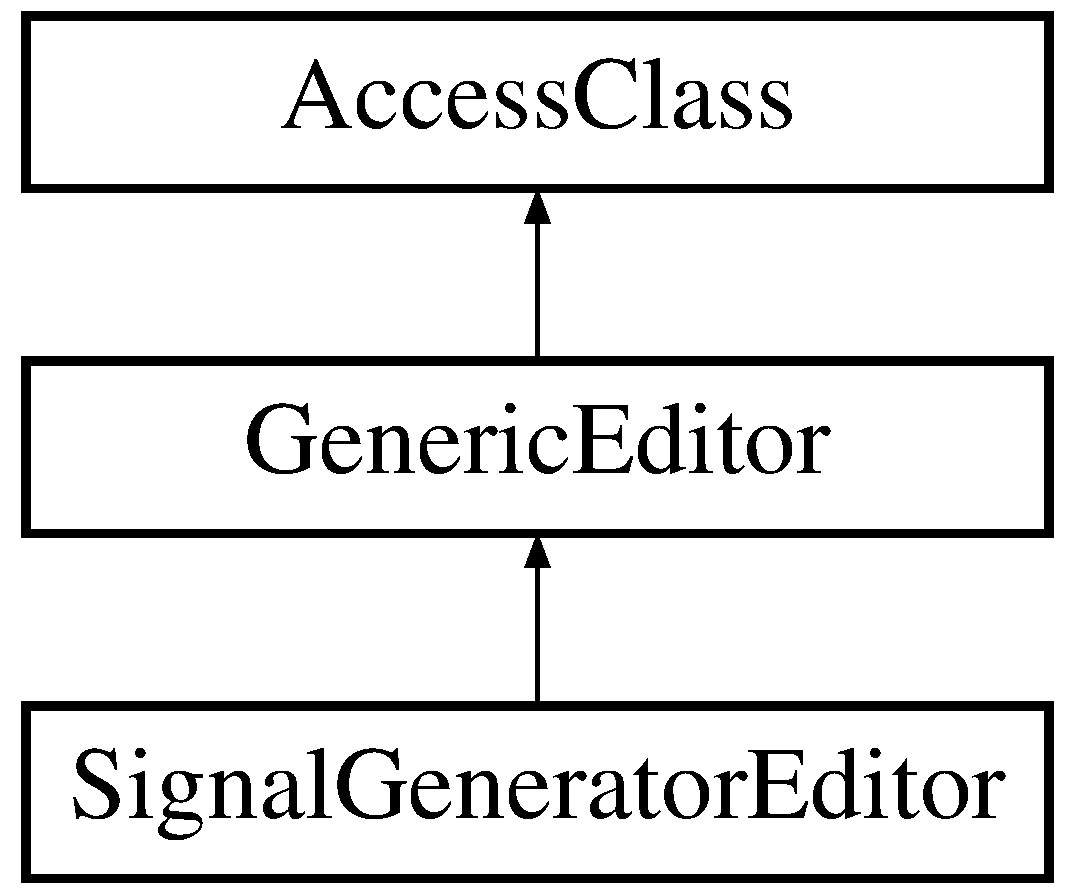
\includegraphics[height=3.000000cm]{classSignalGeneratorEditor}
\end{center}
\end{figure}
\subsection*{Public Member Functions}
\begin{DoxyCompactItemize}
\item 
\hypertarget{classSignalGeneratorEditor_aac0fcfad0aaefec4768919f0e7f1eebb}{{\bfseries Signal\-Generator\-Editor} (\hyperlink{classGenericProcessor}{Generic\-Processor} $\ast$parent\-Node)}\label{classSignalGeneratorEditor_aac0fcfad0aaefec4768919f0e7f1eebb}

\item 
\hypertarget{classSignalGeneratorEditor_a73b886e45b124f62f6bd4b9eafb551b6}{void {\bfseries slider\-Event} (Slider $\ast$slider)}\label{classSignalGeneratorEditor_a73b886e45b124f62f6bd4b9eafb551b6}

\item 
\hypertarget{classSignalGeneratorEditor_a6d9ab33c5fbc544e442e5d30838bd9cd}{void {\bfseries button\-Event} (Button $\ast$button)}\label{classSignalGeneratorEditor_a6d9ab33c5fbc544e442e5d30838bd9cd}

\item 
\hypertarget{classSignalGeneratorEditor_ac06bf3a2d62e274605e65a60edaa72bc}{void {\bfseries label\-Text\-Changed} (Label $\ast$label)}\label{classSignalGeneratorEditor_ac06bf3a2d62e274605e65a60edaa72bc}

\item 
\hypertarget{classSignalGeneratorEditor_a68b95539ae3f0ebf6a900196a3070236}{void {\bfseries add\-Parameter\-Editors} ()}\label{classSignalGeneratorEditor_a68b95539ae3f0ebf6a900196a3070236}

\end{DoxyCompactItemize}
\subsection*{Private Types}
\begin{DoxyCompactItemize}
\item 
enum {\bfseries wvfrm} \{ \\*
{\bfseries S\-I\-N\-E}, 
{\bfseries S\-Q\-U\-A\-R\-E}, 
{\bfseries S\-A\-W}, 
{\bfseries T\-R\-I\-A\-N\-G\-L\-E}, 
\\*
{\bfseries N\-O\-I\-S\-E}
 \}
\end{DoxyCompactItemize}
\subsection*{Private Member Functions}
\begin{DoxyCompactItemize}
\item 
\hypertarget{classSignalGeneratorEditor_a3583ca3f8821c4ed4885d0f84d07468d}{{\bfseries J\-U\-C\-E\-\_\-\-D\-E\-C\-L\-A\-R\-E\-\_\-\-N\-O\-N\-\_\-\-C\-O\-P\-Y\-A\-B\-L\-E\-\_\-\-W\-I\-T\-H\-\_\-\-L\-E\-A\-K\-\_\-\-D\-E\-T\-E\-C\-T\-O\-R} (\hyperlink{classSignalGeneratorEditor}{Signal\-Generator\-Editor})}\label{classSignalGeneratorEditor_a3583ca3f8821c4ed4885d0f84d07468d}

\end{DoxyCompactItemize}
\subsection*{Private Attributes}
\begin{DoxyCompactItemize}
\item 
\hypertarget{classSignalGeneratorEditor_acda38d4cb291a20bfab5ce2d5013b5ae}{Label $\ast$ {\bfseries num\-Channels\-Label}}\label{classSignalGeneratorEditor_acda38d4cb291a20bfab5ce2d5013b5ae}

\item 
\hypertarget{classSignalGeneratorEditor_a132c2da3204548423cb5dcc5d352a710}{\hyperlink{classTriangleButton}{Triangle\-Button} $\ast$ {\bfseries up\-Button}}\label{classSignalGeneratorEditor_a132c2da3204548423cb5dcc5d352a710}

\item 
\hypertarget{classSignalGeneratorEditor_ae57418a3331d72315e0250e43622c01c}{\hyperlink{classTriangleButton}{Triangle\-Button} $\ast$ {\bfseries down\-Button}}\label{classSignalGeneratorEditor_ae57418a3331d72315e0250e43622c01c}

\item 
\hypertarget{classSignalGeneratorEditor_ac2499b00e668b3aeab63a09eb1a2c89e}{Slider $\ast$ {\bfseries amplitude\-Slider}}\label{classSignalGeneratorEditor_ac2499b00e668b3aeab63a09eb1a2c89e}

\item 
\hypertarget{classSignalGeneratorEditor_a3073b75e76f4cbe8b4dee2caaa4fcd8b}{Slider $\ast$ {\bfseries frequency\-Slider}}\label{classSignalGeneratorEditor_a3073b75e76f4cbe8b4dee2caaa4fcd8b}

\item 
\hypertarget{classSignalGeneratorEditor_a759d6577546094b3a90e0bd5c152affe}{Slider $\ast$ {\bfseries phase\-Slider}}\label{classSignalGeneratorEditor_a759d6577546094b3a90e0bd5c152affe}

\item 
\hypertarget{classSignalGeneratorEditor_aad965f7f052bf9840044edac2699fc3a}{Array$<$ \hyperlink{classWaveformSelector}{Waveform\-Selector} $\ast$ $>$ {\bfseries waveform\-Selectors}}\label{classSignalGeneratorEditor_aad965f7f052bf9840044edac2699fc3a}

\end{DoxyCompactItemize}
\subsection*{Additional Inherited Members}


The documentation for this class was generated from the following file\-:\begin{DoxyCompactItemize}
\item 
Processors/\-Editors/Signal\-Generator\-Editor.\-h\end{DoxyCompactItemize}

\hypertarget{structSimpleKeyEvent}{\section{Simple\-Key\-Event Struct Reference}
\label{structSimpleKeyEvent}\index{Simple\-Key\-Event@{Simple\-Key\-Event}}
}
\subsection*{Public Attributes}
\begin{DoxyCompactItemize}
\item 
\hypertarget{structSimpleKeyEvent_ac3f519a65f1b8bc757ca8560a3c1a4f0}{int {\bfseries key}}\label{structSimpleKeyEvent_ac3f519a65f1b8bc757ca8560a3c1a4f0}

\item 
\hypertarget{structSimpleKeyEvent_adf840a9b2662f5e709ee40e245e988ad}{bool {\bfseries shift}}\label{structSimpleKeyEvent_adf840a9b2662f5e709ee40e245e988ad}

\item 
\hypertarget{structSimpleKeyEvent_a594a56922b5f00a178d7abb76ae43c02}{bool {\bfseries ctrl}}\label{structSimpleKeyEvent_a594a56922b5f00a178d7abb76ae43c02}

\item 
\hypertarget{structSimpleKeyEvent_aec2639c73f1ee6fff8f894ccd6454a3f}{bool {\bfseries alt}}\label{structSimpleKeyEvent_aec2639c73f1ee6fff8f894ccd6454a3f}

\end{DoxyCompactItemize}


The documentation for this struct was generated from the following file\-:\begin{DoxyCompactItemize}
\item 
Processors/\-Visualization/\-Spike\-Plotting/Simple\-Key\-Event.\-h\end{DoxyCompactItemize}

\hypertarget{classSourceNode}{\section{Source\-Node Class Reference}
\label{classSourceNode}\index{Source\-Node@{Source\-Node}}
}


{\ttfamily \#include $<$Source\-Node.\-h$>$}

Inheritance diagram for Source\-Node\-:\begin{figure}[H]
\begin{center}
\leavevmode
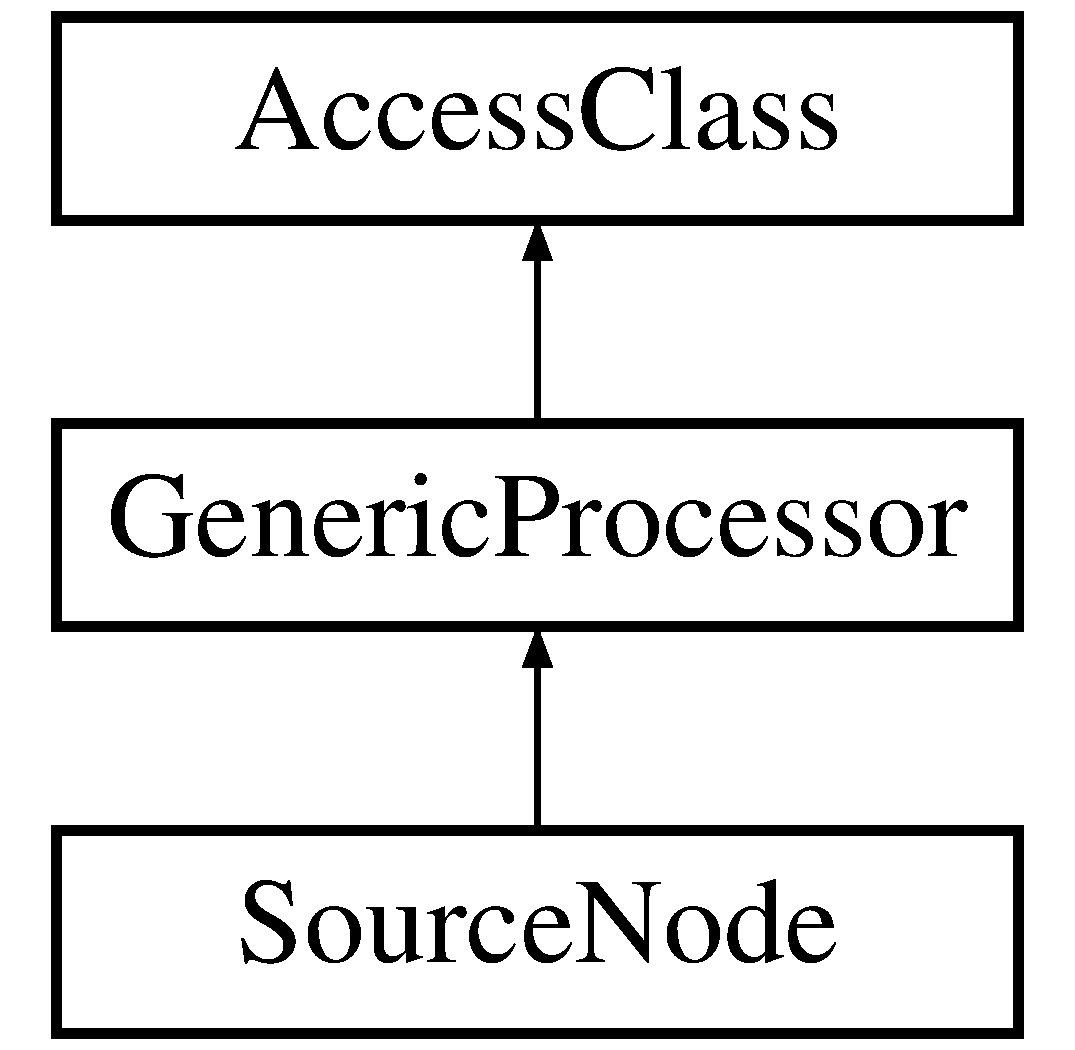
\includegraphics[height=3.000000cm]{classSourceNode}
\end{center}
\end{figure}
\subsection*{Public Member Functions}
\begin{DoxyCompactItemize}
\item 
\hypertarget{classSourceNode_ab4f329f2c043ff22b7111b2d4f858914}{{\bfseries Source\-Node} (const String \&name)}\label{classSourceNode_ab4f329f2c043ff22b7111b2d4f858914}

\item 
\hypertarget{classSourceNode_af79d18af3b7ccc5d429ec9821c8ed8e0}{void {\bfseries enabled\-State} (bool t)}\label{classSourceNode_af79d18af3b7ccc5d429ec9821c8ed8e0}

\item 
\hypertarget{classSourceNode_a7878b4b9142e39d9bf2ffc583ba09330}{void {\bfseries process} (Audio\-Sample\-Buffer \&buffer, Midi\-Buffer \&midi\-Messages, int \&n\-Samples)}\label{classSourceNode_a7878b4b9142e39d9bf2ffc583ba09330}

\item 
\hypertarget{classSourceNode_a188872e7c56ea9d8408228632cedd95d}{void {\bfseries set\-Parameter} (int parameter\-Index, float new\-Value)}\label{classSourceNode_a188872e7c56ea9d8408228632cedd95d}

\item 
\hypertarget{classSourceNode_a777f8795ab9dc3c9561e60bdcef6a9bb}{float {\bfseries get\-Sample\-Rate} ()}\label{classSourceNode_a777f8795ab9dc3c9561e60bdcef6a9bb}

\item 
\hypertarget{classSourceNode_acaf6815c0144908b659752e474fb1f4e}{float {\bfseries get\-Default\-Sample\-Rate} ()}\label{classSourceNode_acaf6815c0144908b659752e474fb1f4e}

\item 
\hypertarget{classSourceNode_a17ba5887e1fea781462df6225b9b5e0f}{int {\bfseries get\-Default\-Num\-Outputs} ()}\label{classSourceNode_a17ba5887e1fea781462df6225b9b5e0f}

\item 
\hypertarget{classSourceNode_abb6c608b0619608c92985fb3bceef43e}{float {\bfseries get\-Default\-Bit\-Volts} ()}\label{classSourceNode_abb6c608b0619608c92985fb3bceef43e}

\item 
\hypertarget{classSourceNode_a7359ff763096c94605c022b528a66382}{Audio\-Processor\-Editor $\ast$ {\bfseries create\-Editor} ()}\label{classSourceNode_a7359ff763096c94605c022b528a66382}

\item 
\hypertarget{classSourceNode_a9bad4ed9244b490448b712776ff78123}{bool {\bfseries has\-Editor} () const }\label{classSourceNode_a9bad4ed9244b490448b712776ff78123}

\item 
\hypertarget{classSourceNode_a34ef124baa3dd9d3d94f92a8ce40dd94}{bool {\bfseries enable} ()}\label{classSourceNode_a34ef124baa3dd9d3d94f92a8ce40dd94}

\item 
\hypertarget{classSourceNode_ab611b02d5535aa01cdebc0fea95f349e}{bool {\bfseries disable} ()}\label{classSourceNode_ab611b02d5535aa01cdebc0fea95f349e}

\item 
\hypertarget{classSourceNode_aac2b14b5eb996f44bb81ea0a097ec1d5}{bool {\bfseries is\-Ready} ()}\label{classSourceNode_aac2b14b5eb996f44bb81ea0a097ec1d5}

\item 
\hypertarget{classSourceNode_a08d7383fb2cae095356c45ed91d491ad}{bool {\bfseries is\-Source} ()}\label{classSourceNode_a08d7383fb2cae095356c45ed91d491ad}

\item 
\hypertarget{classSourceNode_ab86697fbc4618026ce0a51087f9537b9}{void {\bfseries acquisition\-Stopped} ()}\label{classSourceNode_ab86697fbc4618026ce0a51087f9537b9}

\end{DoxyCompactItemize}
\subsection*{Private Member Functions}
\begin{DoxyCompactItemize}
\item 
\hypertarget{classSourceNode_ac0529c95b1179f9a62d9d3d5b94e4a54}{void {\bfseries timer\-Callback} ()}\label{classSourceNode_ac0529c95b1179f9a62d9d3d5b94e4a54}

\item 
\hypertarget{classSourceNode_acda032e8fe961d76456ea81913892627}{void {\bfseries update\-Settings} ()}\label{classSourceNode_acda032e8fe961d76456ea81913892627}

\item 
\hypertarget{classSourceNode_a363a1e41e163aa2373f81a006be110bf}{{\bfseries J\-U\-C\-E\-\_\-\-D\-E\-C\-L\-A\-R\-E\-\_\-\-N\-O\-N\-\_\-\-C\-O\-P\-Y\-A\-B\-L\-E\-\_\-\-W\-I\-T\-H\-\_\-\-L\-E\-A\-K\-\_\-\-D\-E\-T\-E\-C\-T\-O\-R} (\hyperlink{classSourceNode}{Source\-Node})}\label{classSourceNode_a363a1e41e163aa2373f81a006be110bf}

\end{DoxyCompactItemize}
\subsection*{Private Attributes}
\begin{DoxyCompactItemize}
\item 
\hypertarget{classSourceNode_a41ccf1b5806b6ce87f830120089302b7}{int {\bfseries source\-Check\-Interval}}\label{classSourceNode_a41ccf1b5806b6ce87f830120089302b7}

\item 
\hypertarget{classSourceNode_aa29195288c1bf19bd692e2ef4f44a262}{bool {\bfseries was\-Disabled}}\label{classSourceNode_aa29195288c1bf19bd692e2ef4f44a262}

\item 
\hypertarget{classSourceNode_ae6fb14e27892f11368f1951c7c34b275}{Scoped\-Pointer$<$ \hyperlink{classDataThread}{Data\-Thread} $>$ {\bfseries data\-Thread}}\label{classSourceNode_ae6fb14e27892f11368f1951c7c34b275}

\item 
\hypertarget{classSourceNode_a4fe4bcde50cf6efe07c199a648e5bc6b}{\hyperlink{classDataBuffer}{Data\-Buffer} $\ast$ {\bfseries input\-Buffer}}\label{classSourceNode_a4fe4bcde50cf6efe07c199a648e5bc6b}

\item 
\hypertarget{classSourceNode_a3fbec02fc3223e1e982db3867323538f}{int $\ast$ {\bfseries num\-Samples\-In\-This\-Buffer}}\label{classSourceNode_a3fbec02fc3223e1e982db3867323538f}

\end{DoxyCompactItemize}
\subsection*{Additional Inherited Members}


\subsection{Detailed Description}
Creates and controls a thread for reading data from external sources.

\begin{DoxySeeAlso}{See also}
\hyperlink{classGenericProcessor}{Generic\-Processor}, \hyperlink{classSourceNodeEditor}{Source\-Node\-Editor}, \hyperlink{classDataThread}{Data\-Thread}, \hyperlink{classIntanThread}{Intan\-Thread} 
\end{DoxySeeAlso}


The documentation for this class was generated from the following file\-:\begin{DoxyCompactItemize}
\item 
Processors/Source\-Node.\-h\end{DoxyCompactItemize}

\hypertarget{classSourceNodeEditor}{\section{Source\-Node\-Editor Class Reference}
\label{classSourceNodeEditor}\index{Source\-Node\-Editor@{Source\-Node\-Editor}}
}
Inheritance diagram for Source\-Node\-Editor\-:\begin{figure}[H]
\begin{center}
\leavevmode
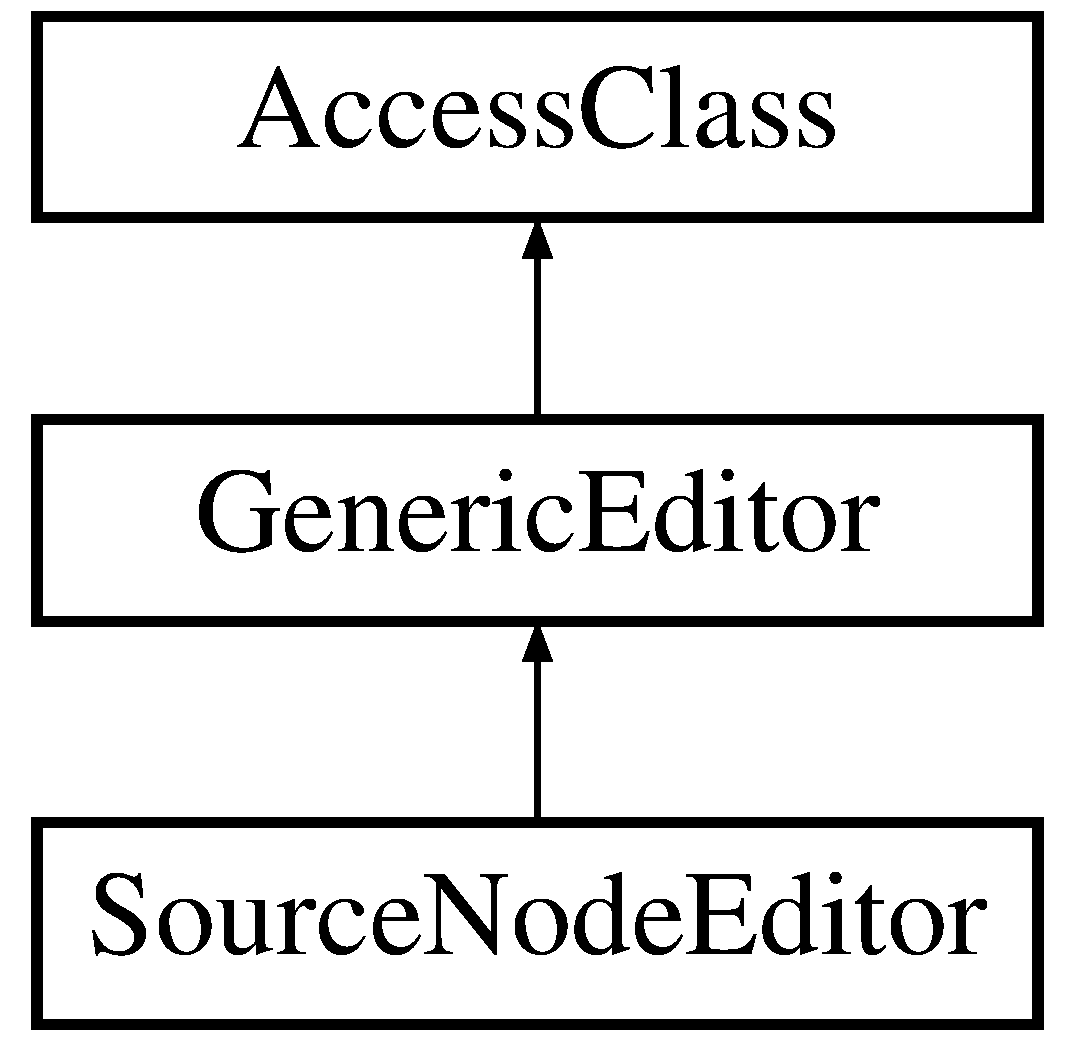
\includegraphics[height=3.000000cm]{classSourceNodeEditor}
\end{center}
\end{figure}
\subsection*{Public Member Functions}
\begin{DoxyCompactItemize}
\item 
\hypertarget{classSourceNodeEditor_af74a126037071a0c7fd2030002248be2}{{\bfseries Source\-Node\-Editor} (\hyperlink{classGenericProcessor}{Generic\-Processor} $\ast$parent\-Node)}\label{classSourceNodeEditor_af74a126037071a0c7fd2030002248be2}

\end{DoxyCompactItemize}
\subsection*{Private Member Functions}
\begin{DoxyCompactItemize}
\item 
\hypertarget{classSourceNodeEditor_a40ac7dcad332a57a292e69cc9aaf6232}{{\bfseries J\-U\-C\-E\-\_\-\-D\-E\-C\-L\-A\-R\-E\-\_\-\-N\-O\-N\-\_\-\-C\-O\-P\-Y\-A\-B\-L\-E\-\_\-\-W\-I\-T\-H\-\_\-\-L\-E\-A\-K\-\_\-\-D\-E\-T\-E\-C\-T\-O\-R} (\hyperlink{classSourceNodeEditor}{Source\-Node\-Editor})}\label{classSourceNodeEditor_a40ac7dcad332a57a292e69cc9aaf6232}

\end{DoxyCompactItemize}
\subsection*{Private Attributes}
\begin{DoxyCompactItemize}
\item 
\hypertarget{classSourceNodeEditor_a31670f7b441dfe1d0f639256ac7f0fc6}{\hyperlink{classImageIcon}{Image\-Icon} $\ast$ {\bfseries icon}}\label{classSourceNodeEditor_a31670f7b441dfe1d0f639256ac7f0fc6}

\end{DoxyCompactItemize}
\subsection*{Additional Inherited Members}


The documentation for this class was generated from the following file\-:\begin{DoxyCompactItemize}
\item 
Processors/\-Editors/Source\-Node\-Editor.\-h\end{DoxyCompactItemize}

\hypertarget{classSpikeDetector}{\section{Spike\-Detector Class Reference}
\label{classSpikeDetector}\index{Spike\-Detector@{Spike\-Detector}}
}
Inheritance diagram for Spike\-Detector\-:\begin{figure}[H]
\begin{center}
\leavevmode
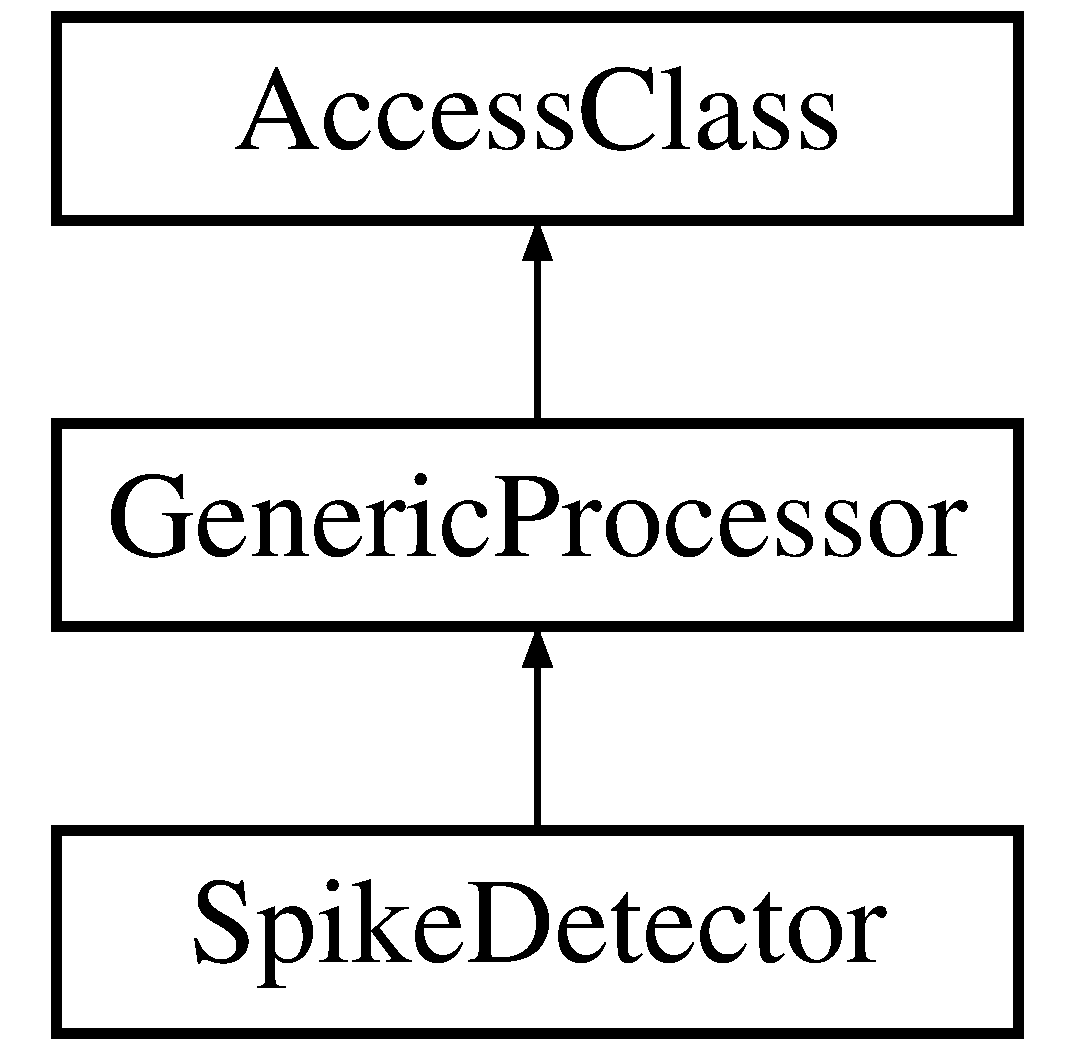
\includegraphics[height=3.000000cm]{classSpikeDetector}
\end{center}
\end{figure}
\subsection*{Classes}
\begin{DoxyCompactItemize}
\item 
struct \hyperlink{structSpikeDetector_1_1Electrode}{Electrode}
\end{DoxyCompactItemize}
\subsection*{Public Member Functions}
\begin{DoxyCompactItemize}
\item 
\hyperlink{classSpikeDetector_a3e3101762b27b1df8be6e8fd1a0bca22}{Spike\-Detector} ()
\item 
\hyperlink{classSpikeDetector_a1cd55b8cabe87b211d7f077ea3003a65}{$\sim$\-Spike\-Detector} ()
\item 
void \hyperlink{classSpikeDetector_a9ba352094475b7be33ca36ae918492d1}{process} (Audio\-Sample\-Buffer \&buffer, Midi\-Buffer \&events, int \&n\-Samples)
\item 
void \hyperlink{classSpikeDetector_a679f5e087dfb959d61f3dd9cdf364cf2}{set\-Parameter} (int parameter\-Index, float new\-Value)
\item 
void \hyperlink{classSpikeDetector_a3c764b20638e3cd2245cab442ce434ca}{update\-Settings} ()
\item 
bool \hyperlink{classSpikeDetector_a50b98fa352359b8dec78b21356c9acbb}{enable} ()
\item 
bool \hyperlink{classSpikeDetector_aeaaac10f4059ee1cdabcff58d24b5f52}{disable} ()
\item 
Audio\-Processor\-Editor $\ast$ \hyperlink{classSpikeDetector_af96da67cfafdba1e59b7eb88b3ed0de6}{create\-Editor} ()
\item 
bool \hyperlink{classSpikeDetector_a59b4ac520a1831ecd5e02df4a58e6735}{add\-Electrode} (int n\-Chans)
\item 
bool \hyperlink{classSpikeDetector_ae05d17ef7b8706a370d4d7e049cec877}{remove\-Electrode} (int index)
\item 
int \hyperlink{classSpikeDetector_a2e5115a6d0508a3476601856eab7ebbe}{get\-Num\-Channels} (int index)
\item 
bool \hyperlink{classSpikeDetector_a44be956ab12ff6a6d69ad90dd732ad51}{set\-Channel} (int electrode\-Index, int channel\-Num, int new\-Channel)
\item 
int \hyperlink{classSpikeDetector_ad43da7a9241a36b6d04c99c6821752d9}{get\-Channel} (int index, int chan)
\item 
bool \hyperlink{classSpikeDetector_a41023a894e0d32db949a823b469eb4d6}{set\-Electrode\-Name} (int index, String new\-Name)
\item 
String\-Array \hyperlink{classSpikeDetector_a6acb52a82fec95ad7b44cf2584fcdc0d}{get\-Electrode\-Names} ()
\item 
\hypertarget{classSpikeDetector_a6fc7b97799e3c1d6d4841d489b8bc854}{void {\bfseries set\-Channel\-Threshold} (int electrode\-Num, int channel\-Num, float threshold)}\label{classSpikeDetector_a6fc7b97799e3c1d6d4841d489b8bc854}

\item 
\hypertarget{classSpikeDetector_aa00bc3a6b29da73fdc75517579289b13}{double {\bfseries get\-Channel\-Threshold} (int electrode\-Num, int channel\-Num)}\label{classSpikeDetector_aa00bc3a6b29da73fdc75517579289b13}

\end{DoxyCompactItemize}
\subsection*{Public Attributes}
\begin{DoxyCompactItemize}
\item 
Audio\-Sample\-Buffer \hyperlink{classSpikeDetector_a789328f70cc6f1de8f0b862189ce23bd}{overflow\-Buffer}
\item 
Audio\-Sample\-Buffer \& \hyperlink{classSpikeDetector_a050b87d647b7d12dd76e6e4fde9f932f}{data\-Buffer}
\item 
String\-Array \hyperlink{classSpikeDetector_a23eaf5359b4d13f75a16a28190014619}{electrode\-Types}
\end{DoxyCompactItemize}
\subsection*{Private Member Functions}
\begin{DoxyCompactItemize}
\item 
\hypertarget{classSpikeDetector_a7c562f7bf7f40e605a5e157ee1e7cdcd}{float {\bfseries get\-Default\-Threshold} ()}\label{classSpikeDetector_a7c562f7bf7f40e605a5e157ee1e7cdcd}

\item 
\hypertarget{classSpikeDetector_aada970694c2dfca0f446efade94f7c86}{float {\bfseries get\-Next\-Sample} (int \&chan)}\label{classSpikeDetector_aada970694c2dfca0f446efade94f7c86}

\item 
\hypertarget{classSpikeDetector_af2792d58c9cf0685b082b055df685761}{float {\bfseries get\-Current\-Sample} (int \&chan)}\label{classSpikeDetector_af2792d58c9cf0685b082b055df685761}

\item 
\hypertarget{classSpikeDetector_adcc1f42731e9b6b48ab089a07dde86f3}{bool {\bfseries samples\-Available} (int \&n\-Samples)}\label{classSpikeDetector_adcc1f42731e9b6b48ab089a07dde86f3}

\item 
\hypertarget{classSpikeDetector_a209554bc3445b84c9c8bad5301385da8}{void {\bfseries add\-Spike\-Event} (\hyperlink{structSpikeObject}{Spike\-Object} $\ast$s, Midi\-Buffer \&event\-Buffer, int peak\-Index)}\label{classSpikeDetector_a209554bc3445b84c9c8bad5301385da8}

\item 
\hypertarget{classSpikeDetector_aad6ba0205c76fec7aa84769937e24ef9}{void {\bfseries add\-Waveform\-To\-Spike\-Object} (\hyperlink{structSpikeObject}{Spike\-Object} $\ast$s, int \&peak\-Index, int \&electrode\-Number, int \&current\-Channel)}\label{classSpikeDetector_aad6ba0205c76fec7aa84769937e24ef9}

\item 
\hypertarget{classSpikeDetector_a779cd2ac50c56febd836d9aaddbdcd5a}{void {\bfseries reset\-Electrode} (\hyperlink{structSpikeDetector_1_1Electrode}{Electrode} $\ast$)}\label{classSpikeDetector_a779cd2ac50c56febd836d9aaddbdcd5a}

\item 
\hypertarget{classSpikeDetector_a8fb28af27a5b3b47d69faacec0f73c41}{{\bfseries J\-U\-C\-E\-\_\-\-D\-E\-C\-L\-A\-R\-E\-\_\-\-N\-O\-N\-\_\-\-C\-O\-P\-Y\-A\-B\-L\-E\-\_\-\-W\-I\-T\-H\-\_\-\-L\-E\-A\-K\-\_\-\-D\-E\-T\-E\-C\-T\-O\-R} (\hyperlink{classSpikeDetector}{Spike\-Detector})}\label{classSpikeDetector_a8fb28af27a5b3b47d69faacec0f73c41}

\end{DoxyCompactItemize}
\subsection*{Private Attributes}
\begin{DoxyCompactItemize}
\item 
\hypertarget{classSpikeDetector_a9bb9fe494706442edbe6f95556c92230}{int {\bfseries overflow\-Buffer\-Size}}\label{classSpikeDetector_a9bb9fe494706442edbe6f95556c92230}

\item 
\hypertarget{classSpikeDetector_a744815ecabf7d3dff9c654a57ee11259}{int {\bfseries sample\-Index}}\label{classSpikeDetector_a744815ecabf7d3dff9c654a57ee11259}

\item 
\hypertarget{classSpikeDetector_a45c1e8ff8c6a8c5f531ca496e41009a9}{Array$<$ int $>$ {\bfseries electrode\-Counter}}\label{classSpikeDetector_a45c1e8ff8c6a8c5f531ca496e41009a9}

\item 
\hypertarget{classSpikeDetector_ab718028e4e8bc0d4fa094d84c38bb50b}{bool {\bfseries use\-Overflow\-Buffer}}\label{classSpikeDetector_ab718028e4e8bc0d4fa094d84c38bb50b}

\item 
\hypertarget{classSpikeDetector_ab0519461dcd76c40bbfc535ebaeb17cf}{int {\bfseries current\-Electrode}}\label{classSpikeDetector_ab0519461dcd76c40bbfc535ebaeb17cf}

\item 
\hypertarget{classSpikeDetector_a0deaa79b22ff4b1516961ee8c1806883}{int {\bfseries current\-Channel\-Index}}\label{classSpikeDetector_a0deaa79b22ff4b1516961ee8c1806883}

\item 
\hypertarget{classSpikeDetector_a06af1d21348b9a71f22b59f36e5c013c}{int {\bfseries current\-Index}}\label{classSpikeDetector_a06af1d21348b9a71f22b59f36e5c013c}

\item 
\hypertarget{classSpikeDetector_a89bb86011a66eebed04fbb48f62768e8}{uint8\-\_\-t $\ast$ {\bfseries spike\-Buffer}}\label{classSpikeDetector_a89bb86011a66eebed04fbb48f62768e8}

\item 
\hypertarget{classSpikeDetector_a40e46503e06199b8366f2f02c064f388}{Array$<$ \hyperlink{structSpikeDetector_1_1Electrode}{Electrode} $\ast$ $>$ \hyperlink{classSpikeDetector_a40e46503e06199b8366f2f02c064f388}{electrodes}}\label{classSpikeDetector_a40e46503e06199b8366f2f02c064f388}

\begin{DoxyCompactList}\small\item\em \mbox{[}256\mbox{]}; \end{DoxyCompactList}\end{DoxyCompactItemize}
\subsection*{Additional Inherited Members}


\subsection{Constructor \& Destructor Documentation}
\hypertarget{classSpikeDetector_a3e3101762b27b1df8be6e8fd1a0bca22}{\index{Spike\-Detector@{Spike\-Detector}!Spike\-Detector@{Spike\-Detector}}
\index{Spike\-Detector@{Spike\-Detector}!SpikeDetector@{Spike\-Detector}}
\subsubsection[{Spike\-Detector}]{\setlength{\rightskip}{0pt plus 5cm}Spike\-Detector\-::\-Spike\-Detector (
\begin{DoxyParamCaption}
{}
\end{DoxyParamCaption}
)}}\label{classSpikeDetector_a3e3101762b27b1df8be6e8fd1a0bca22}
constructor \hypertarget{classSpikeDetector_a1cd55b8cabe87b211d7f077ea3003a65}{\index{Spike\-Detector@{Spike\-Detector}!$\sim$\-Spike\-Detector@{$\sim$\-Spike\-Detector}}
\index{$\sim$\-Spike\-Detector@{$\sim$\-Spike\-Detector}!SpikeDetector@{Spike\-Detector}}
\subsubsection[{$\sim$\-Spike\-Detector}]{\setlength{\rightskip}{0pt plus 5cm}Spike\-Detector\-::$\sim$\-Spike\-Detector (
\begin{DoxyParamCaption}
{}
\end{DoxyParamCaption}
)}}\label{classSpikeDetector_a1cd55b8cabe87b211d7f077ea3003a65}
destructor 

\subsection{Member Function Documentation}
\hypertarget{classSpikeDetector_a59b4ac520a1831ecd5e02df4a58e6735}{\index{Spike\-Detector@{Spike\-Detector}!add\-Electrode@{add\-Electrode}}
\index{add\-Electrode@{add\-Electrode}!SpikeDetector@{Spike\-Detector}}
\subsubsection[{add\-Electrode}]{\setlength{\rightskip}{0pt plus 5cm}bool Spike\-Detector\-::add\-Electrode (
\begin{DoxyParamCaption}
\item[{int}]{n\-Chans}
\end{DoxyParamCaption}
)}}\label{classSpikeDetector_a59b4ac520a1831ecd5e02df4a58e6735}
Adds an electrode with n channels to be processed. \hypertarget{classSpikeDetector_af96da67cfafdba1e59b7eb88b3ed0de6}{\index{Spike\-Detector@{Spike\-Detector}!create\-Editor@{create\-Editor}}
\index{create\-Editor@{create\-Editor}!SpikeDetector@{Spike\-Detector}}
\subsubsection[{create\-Editor}]{\setlength{\rightskip}{0pt plus 5cm}Audio\-Processor\-Editor$\ast$ Spike\-Detector\-::create\-Editor (
\begin{DoxyParamCaption}
{}
\end{DoxyParamCaption}
)\hspace{0.3cm}{\ttfamily [virtual]}}}\label{classSpikeDetector_af96da67cfafdba1e59b7eb88b3ed0de6}
Creates the \hyperlink{classSpikeDetectorEditor}{Spike\-Detector\-Editor}. 

Reimplemented from \hyperlink{classGenericProcessor}{Generic\-Processor}.

\hypertarget{classSpikeDetector_aeaaac10f4059ee1cdabcff58d24b5f52}{\index{Spike\-Detector@{Spike\-Detector}!disable@{disable}}
\index{disable@{disable}!SpikeDetector@{Spike\-Detector}}
\subsubsection[{disable}]{\setlength{\rightskip}{0pt plus 5cm}bool Spike\-Detector\-::disable (
\begin{DoxyParamCaption}
{}
\end{DoxyParamCaption}
)\hspace{0.3cm}{\ttfamily [virtual]}}}\label{classSpikeDetector_aeaaac10f4059ee1cdabcff58d24b5f52}
Called after acquisition is finished. 

Reimplemented from \hyperlink{classGenericProcessor}{Generic\-Processor}.

\hypertarget{classSpikeDetector_a50b98fa352359b8dec78b21356c9acbb}{\index{Spike\-Detector@{Spike\-Detector}!enable@{enable}}
\index{enable@{enable}!SpikeDetector@{Spike\-Detector}}
\subsubsection[{enable}]{\setlength{\rightskip}{0pt plus 5cm}bool Spike\-Detector\-::enable (
\begin{DoxyParamCaption}
{}
\end{DoxyParamCaption}
)\hspace{0.3cm}{\ttfamily [virtual]}}}\label{classSpikeDetector_a50b98fa352359b8dec78b21356c9acbb}
Called prior to start of acquisition. 

Reimplemented from \hyperlink{classGenericProcessor}{Generic\-Processor}.

\hypertarget{classSpikeDetector_ad43da7a9241a36b6d04c99c6821752d9}{\index{Spike\-Detector@{Spike\-Detector}!get\-Channel@{get\-Channel}}
\index{get\-Channel@{get\-Channel}!SpikeDetector@{Spike\-Detector}}
\subsubsection[{get\-Channel}]{\setlength{\rightskip}{0pt plus 5cm}int Spike\-Detector\-::get\-Channel (
\begin{DoxyParamCaption}
\item[{int}]{index, }
\item[{int}]{chan}
\end{DoxyParamCaption}
)}}\label{classSpikeDetector_ad43da7a9241a36b6d04c99c6821752d9}
Returns the continuous channel that maps to a given electrode channel. \hypertarget{classSpikeDetector_a6acb52a82fec95ad7b44cf2584fcdc0d}{\index{Spike\-Detector@{Spike\-Detector}!get\-Electrode\-Names@{get\-Electrode\-Names}}
\index{get\-Electrode\-Names@{get\-Electrode\-Names}!SpikeDetector@{Spike\-Detector}}
\subsubsection[{get\-Electrode\-Names}]{\setlength{\rightskip}{0pt plus 5cm}String\-Array Spike\-Detector\-::get\-Electrode\-Names (
\begin{DoxyParamCaption}
{}
\end{DoxyParamCaption}
)}}\label{classSpikeDetector_a6acb52a82fec95ad7b44cf2584fcdc0d}
Returns a String\-Array containing the names of all electrodes \hypertarget{classSpikeDetector_a2e5115a6d0508a3476601856eab7ebbe}{\index{Spike\-Detector@{Spike\-Detector}!get\-Num\-Channels@{get\-Num\-Channels}}
\index{get\-Num\-Channels@{get\-Num\-Channels}!SpikeDetector@{Spike\-Detector}}
\subsubsection[{get\-Num\-Channels}]{\setlength{\rightskip}{0pt plus 5cm}int Spike\-Detector\-::get\-Num\-Channels (
\begin{DoxyParamCaption}
\item[{int}]{index}
\end{DoxyParamCaption}
)}}\label{classSpikeDetector_a2e5115a6d0508a3476601856eab7ebbe}
Returns the number of channels for a given electrode. \hypertarget{classSpikeDetector_a9ba352094475b7be33ca36ae918492d1}{\index{Spike\-Detector@{Spike\-Detector}!process@{process}}
\index{process@{process}!SpikeDetector@{Spike\-Detector}}
\subsubsection[{process}]{\setlength{\rightskip}{0pt plus 5cm}void Spike\-Detector\-::process (
\begin{DoxyParamCaption}
\item[{Audio\-Sample\-Buffer \&}]{buffer, }
\item[{Midi\-Buffer \&}]{events, }
\item[{int \&}]{n\-Samples}
\end{DoxyParamCaption}
)\hspace{0.3cm}{\ttfamily [virtual]}}}\label{classSpikeDetector_a9ba352094475b7be33ca36ae918492d1}
Processes an incoming continuous buffer and places new spikes into the event buffer. 

Implements \hyperlink{classGenericProcessor}{Generic\-Processor}.

\hypertarget{classSpikeDetector_ae05d17ef7b8706a370d4d7e049cec877}{\index{Spike\-Detector@{Spike\-Detector}!remove\-Electrode@{remove\-Electrode}}
\index{remove\-Electrode@{remove\-Electrode}!SpikeDetector@{Spike\-Detector}}
\subsubsection[{remove\-Electrode}]{\setlength{\rightskip}{0pt plus 5cm}bool Spike\-Detector\-::remove\-Electrode (
\begin{DoxyParamCaption}
\item[{int}]{index}
\end{DoxyParamCaption}
)}}\label{classSpikeDetector_ae05d17ef7b8706a370d4d7e049cec877}
Removes an electrode with a given index. \hypertarget{classSpikeDetector_a44be956ab12ff6a6d69ad90dd732ad51}{\index{Spike\-Detector@{Spike\-Detector}!set\-Channel@{set\-Channel}}
\index{set\-Channel@{set\-Channel}!SpikeDetector@{Spike\-Detector}}
\subsubsection[{set\-Channel}]{\setlength{\rightskip}{0pt plus 5cm}bool Spike\-Detector\-::set\-Channel (
\begin{DoxyParamCaption}
\item[{int}]{electrode\-Index, }
\item[{int}]{channel\-Num, }
\item[{int}]{new\-Channel}
\end{DoxyParamCaption}
)}}\label{classSpikeDetector_a44be956ab12ff6a6d69ad90dd732ad51}
Edits the mapping between input channels and electrode channels. \hypertarget{classSpikeDetector_a41023a894e0d32db949a823b469eb4d6}{\index{Spike\-Detector@{Spike\-Detector}!set\-Electrode\-Name@{set\-Electrode\-Name}}
\index{set\-Electrode\-Name@{set\-Electrode\-Name}!SpikeDetector@{Spike\-Detector}}
\subsubsection[{set\-Electrode\-Name}]{\setlength{\rightskip}{0pt plus 5cm}bool Spike\-Detector\-::set\-Electrode\-Name (
\begin{DoxyParamCaption}
\item[{int}]{index, }
\item[{String}]{new\-Name}
\end{DoxyParamCaption}
)}}\label{classSpikeDetector_a41023a894e0d32db949a823b469eb4d6}
Sets the name of a given electrode. \hypertarget{classSpikeDetector_a679f5e087dfb959d61f3dd9cdf364cf2}{\index{Spike\-Detector@{Spike\-Detector}!set\-Parameter@{set\-Parameter}}
\index{set\-Parameter@{set\-Parameter}!SpikeDetector@{Spike\-Detector}}
\subsubsection[{set\-Parameter}]{\setlength{\rightskip}{0pt plus 5cm}void Spike\-Detector\-::set\-Parameter (
\begin{DoxyParamCaption}
\item[{int}]{parameter\-Index, }
\item[{float}]{new\-Value}
\end{DoxyParamCaption}
)\hspace{0.3cm}{\ttfamily [virtual]}}}\label{classSpikeDetector_a679f5e087dfb959d61f3dd9cdf364cf2}
Used to alter parameters of data acquisition. 

Reimplemented from \hyperlink{classGenericProcessor}{Generic\-Processor}.

\hypertarget{classSpikeDetector_a3c764b20638e3cd2245cab442ce434ca}{\index{Spike\-Detector@{Spike\-Detector}!update\-Settings@{update\-Settings}}
\index{update\-Settings@{update\-Settings}!SpikeDetector@{Spike\-Detector}}
\subsubsection[{update\-Settings}]{\setlength{\rightskip}{0pt plus 5cm}void Spike\-Detector\-::update\-Settings (
\begin{DoxyParamCaption}
{}
\end{DoxyParamCaption}
)\hspace{0.3cm}{\ttfamily [virtual]}}}\label{classSpikeDetector_a3c764b20638e3cd2245cab442ce434ca}
Called whenever the signal chain is altered. 

Reimplemented from \hyperlink{classGenericProcessor}{Generic\-Processor}.



\subsection{Member Data Documentation}
\hypertarget{classSpikeDetector_a050b87d647b7d12dd76e6e4fde9f932f}{\index{Spike\-Detector@{Spike\-Detector}!data\-Buffer@{data\-Buffer}}
\index{data\-Buffer@{data\-Buffer}!SpikeDetector@{Spike\-Detector}}
\subsubsection[{data\-Buffer}]{\setlength{\rightskip}{0pt plus 5cm}Audio\-Sample\-Buffer\& Spike\-Detector\-::data\-Buffer}}\label{classSpikeDetector_a050b87d647b7d12dd76e6e4fde9f932f}
Reference to a continuous buffer (for internal use only). \hypertarget{classSpikeDetector_a23eaf5359b4d13f75a16a28190014619}{\index{Spike\-Detector@{Spike\-Detector}!electrode\-Types@{electrode\-Types}}
\index{electrode\-Types@{electrode\-Types}!SpikeDetector@{Spike\-Detector}}
\subsubsection[{electrode\-Types}]{\setlength{\rightskip}{0pt plus 5cm}String\-Array Spike\-Detector\-::electrode\-Types}}\label{classSpikeDetector_a23eaf5359b4d13f75a16a28190014619}
Returns a list of possible electrode types (e.\-g., stereotrode, tetrode). \hypertarget{classSpikeDetector_a789328f70cc6f1de8f0b862189ce23bd}{\index{Spike\-Detector@{Spike\-Detector}!overflow\-Buffer@{overflow\-Buffer}}
\index{overflow\-Buffer@{overflow\-Buffer}!SpikeDetector@{Spike\-Detector}}
\subsubsection[{overflow\-Buffer}]{\setlength{\rightskip}{0pt plus 5cm}Audio\-Sample\-Buffer Spike\-Detector\-::overflow\-Buffer}}\label{classSpikeDetector_a789328f70cc6f1de8f0b862189ce23bd}
Extra samples are placed in this buffer to allow seamless transitions between callbacks. 

The documentation for this class was generated from the following file\-:\begin{DoxyCompactItemize}
\item 
Processors/Spike\-Detector.\-h\end{DoxyCompactItemize}

\hypertarget{classSpikeDetectorEditor}{\section{Spike\-Detector\-Editor Class Reference}
\label{classSpikeDetectorEditor}\index{Spike\-Detector\-Editor@{Spike\-Detector\-Editor}}
}
Inheritance diagram for Spike\-Detector\-Editor\-:\begin{figure}[H]
\begin{center}
\leavevmode
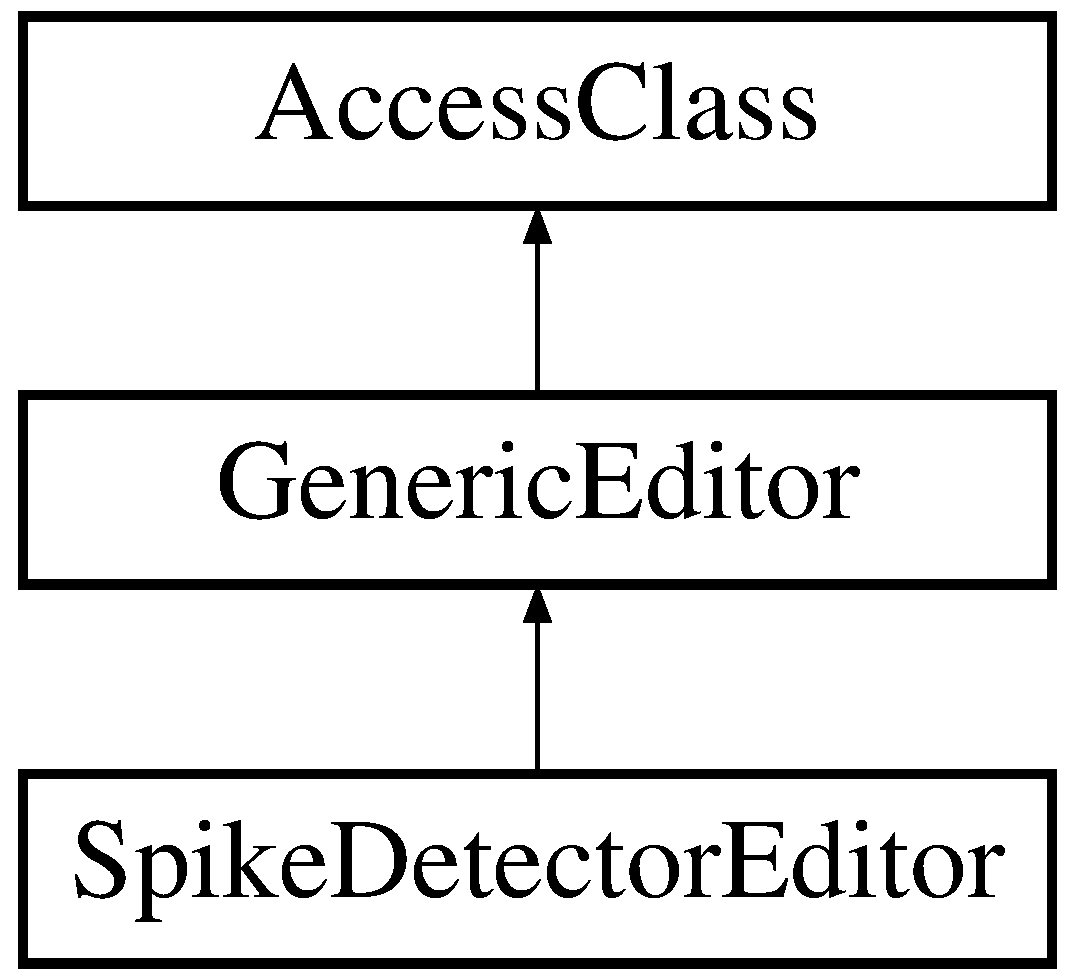
\includegraphics[height=3.000000cm]{classSpikeDetectorEditor}
\end{center}
\end{figure}
\subsection*{Public Member Functions}
\begin{DoxyCompactItemize}
\item 
\hypertarget{classSpikeDetectorEditor_a5e291e45376684d6a7882962c9adbc1b}{{\bfseries Spike\-Detector\-Editor} (\hyperlink{classGenericProcessor}{Generic\-Processor} $\ast$parent\-Node)}\label{classSpikeDetectorEditor_a5e291e45376684d6a7882962c9adbc1b}

\item 
\hypertarget{classSpikeDetectorEditor_a3596a939b1842825ca19c7ba40c45214}{void {\bfseries button\-Event} (Button $\ast$button)}\label{classSpikeDetectorEditor_a3596a939b1842825ca19c7ba40c45214}

\item 
\hypertarget{classSpikeDetectorEditor_ae68515d9c025e06a5f8455a7afeed5bd}{void {\bfseries label\-Text\-Changed} (Label $\ast$label)}\label{classSpikeDetectorEditor_ae68515d9c025e06a5f8455a7afeed5bd}

\item 
\hypertarget{classSpikeDetectorEditor_aa989c11f9a1c54b9a8846512525fa756}{void {\bfseries combo\-Box\-Changed} (Combo\-Box $\ast$combo\-Box)}\label{classSpikeDetectorEditor_aa989c11f9a1c54b9a8846512525fa756}

\item 
\hypertarget{classSpikeDetectorEditor_af44153e6745ac264da123f8c3f97c805}{void {\bfseries slider\-Event} (Slider $\ast$slider)}\label{classSpikeDetectorEditor_af44153e6745ac264da123f8c3f97c805}

\item 
\hypertarget{classSpikeDetectorEditor_a24dcb89b8160a0ee92437ff45309abbb}{void {\bfseries channel\-Changed} (int chan)}\label{classSpikeDetectorEditor_a24dcb89b8160a0ee92437ff45309abbb}

\end{DoxyCompactItemize}
\subsection*{Private Member Functions}
\begin{DoxyCompactItemize}
\item 
\hypertarget{classSpikeDetectorEditor_a8a12482ef358229d2475c60119ecfd2e}{void {\bfseries draw\-Electrode\-Buttons} (int)}\label{classSpikeDetectorEditor_a8a12482ef358229d2475c60119ecfd2e}

\item 
\hypertarget{classSpikeDetectorEditor_a86363456281c79b98c12da2f1c5f36f6}{void {\bfseries refresh\-Electrode\-List} ()}\label{classSpikeDetectorEditor_a86363456281c79b98c12da2f1c5f36f6}

\item 
\hypertarget{classSpikeDetectorEditor_a3478bc7c45b115a1e9a913ba525668ff}{bool {\bfseries add\-Electrode} (int n\-Chans)}\label{classSpikeDetectorEditor_a3478bc7c45b115a1e9a913ba525668ff}

\item 
\hypertarget{classSpikeDetectorEditor_a9c44e850937729a2e7964ddf3d5d83fc}{void {\bfseries remove\-Electrode} (int index)}\label{classSpikeDetectorEditor_a9c44e850937729a2e7964ddf3d5d83fc}

\item 
\hypertarget{classSpikeDetectorEditor_a689d1c5f9f678f25e125c97bf45af10e}{void {\bfseries edit\-Electrode} (int index, int chan, int new\-Chan)}\label{classSpikeDetectorEditor_a689d1c5f9f678f25e125c97bf45af10e}

\item 
\hypertarget{classSpikeDetectorEditor_ae4e0d69017db6a0c3d35c44b92306e53}{{\bfseries J\-U\-C\-E\-\_\-\-D\-E\-C\-L\-A\-R\-E\-\_\-\-N\-O\-N\-\_\-\-C\-O\-P\-Y\-A\-B\-L\-E\-\_\-\-W\-I\-T\-H\-\_\-\-L\-E\-A\-K\-\_\-\-D\-E\-T\-E\-C\-T\-O\-R} (\hyperlink{classSpikeDetectorEditor}{Spike\-Detector\-Editor})}\label{classSpikeDetectorEditor_ae4e0d69017db6a0c3d35c44b92306e53}

\end{DoxyCompactItemize}
\subsection*{Private Attributes}
\begin{DoxyCompactItemize}
\item 
\hypertarget{classSpikeDetectorEditor_ac7a692b3b6dade3ca922ac81ad71b9b4}{Combo\-Box $\ast$ {\bfseries electrode\-Types}}\label{classSpikeDetectorEditor_ac7a692b3b6dade3ca922ac81ad71b9b4}

\item 
\hypertarget{classSpikeDetectorEditor_aa9f66444c51d8cfce0eb11e3d4bc6b58}{Combo\-Box $\ast$ {\bfseries electrode\-List}}\label{classSpikeDetectorEditor_aa9f66444c51d8cfce0eb11e3d4bc6b58}

\item 
\hypertarget{classSpikeDetectorEditor_a87ba0f2756961e42017a492d60d60ade}{Label $\ast$ {\bfseries num\-Electrodes}}\label{classSpikeDetectorEditor_a87ba0f2756961e42017a492d60d60ade}

\item 
\hypertarget{classSpikeDetectorEditor_a46f1f4b01189fbcd9394bf2ce8c6def7}{Label $\ast$ {\bfseries threshold\-Label}}\label{classSpikeDetectorEditor_a46f1f4b01189fbcd9394bf2ce8c6def7}

\item 
\hypertarget{classSpikeDetectorEditor_a339c5a295cd9fdfeba2ccbb0f2605970}{\hyperlink{classTriangleButton}{Triangle\-Button} $\ast$ {\bfseries up\-Button}}\label{classSpikeDetectorEditor_a339c5a295cd9fdfeba2ccbb0f2605970}

\item 
\hypertarget{classSpikeDetectorEditor_a10ad05b072e42e48fe673faa7ea8dca3}{\hyperlink{classTriangleButton}{Triangle\-Button} $\ast$ {\bfseries down\-Button}}\label{classSpikeDetectorEditor_a10ad05b072e42e48fe673faa7ea8dca3}

\item 
\hypertarget{classSpikeDetectorEditor_a45fe71c4c33361070e7c626186361215}{\hyperlink{classUtilityButton}{Utility\-Button} $\ast$ {\bfseries plus\-Button}}\label{classSpikeDetectorEditor_a45fe71c4c33361070e7c626186361215}

\item 
\hypertarget{classSpikeDetectorEditor_a928b494b0f3e5cf426eed32dbc633006}{\hyperlink{classThresholdSlider}{Threshold\-Slider} $\ast$ {\bfseries threshold\-Slider}}\label{classSpikeDetectorEditor_a928b494b0f3e5cf426eed32dbc633006}

\item 
\hypertarget{classSpikeDetectorEditor_ac1070794a04b6a319796370d50a85008}{Owned\-Array$<$ \hyperlink{classElectrodeButton}{Electrode\-Button} $>$ {\bfseries electrode\-Buttons}}\label{classSpikeDetectorEditor_ac1070794a04b6a319796370d50a85008}

\item 
\hypertarget{classSpikeDetectorEditor_a8580bea5fc10f1ee194758f88e70ad52}{Array$<$ \hyperlink{classElectrodeEditorButton}{Electrode\-Editor\-Button} $\ast$ $>$ {\bfseries electrode\-Editor\-Buttons}}\label{classSpikeDetectorEditor_a8580bea5fc10f1ee194758f88e70ad52}

\item 
\hypertarget{classSpikeDetectorEditor_add340b6f65bc5dc5ad0139e943bf54fb}{int {\bfseries last\-Id}}\label{classSpikeDetectorEditor_add340b6f65bc5dc5ad0139e943bf54fb}

\item 
\hypertarget{classSpikeDetectorEditor_a37e9442d68c7edd3db553e97edbe4016}{bool {\bfseries is\-Plural}}\label{classSpikeDetectorEditor_a37e9442d68c7edd3db553e97edbe4016}

\item 
\hypertarget{classSpikeDetectorEditor_a182bb0ac31fa20a654d0f13f058639fd}{Font {\bfseries font}}\label{classSpikeDetectorEditor_a182bb0ac31fa20a654d0f13f058639fd}

\end{DoxyCompactItemize}
\subsection*{Additional Inherited Members}


The documentation for this class was generated from the following file\-:\begin{DoxyCompactItemize}
\item 
Processors/\-Editors/Spike\-Detector\-Editor.\-h\end{DoxyCompactItemize}

\hypertarget{classSpikeDisplayCanvas}{\section{Spike\-Display\-Canvas Class Reference}
\label{classSpikeDisplayCanvas}\index{Spike\-Display\-Canvas@{Spike\-Display\-Canvas}}
}
Inheritance diagram for Spike\-Display\-Canvas\-:\begin{figure}[H]
\begin{center}
\leavevmode
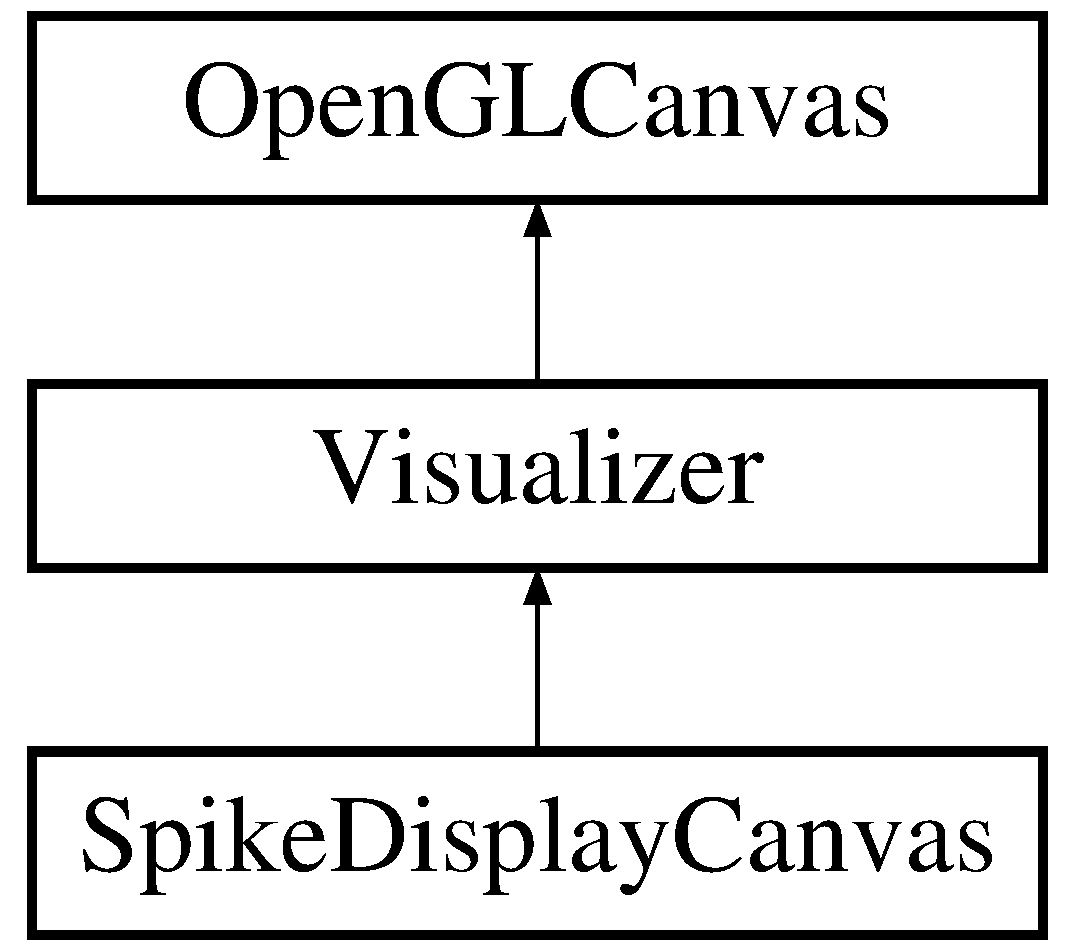
\includegraphics[height=3.000000cm]{classSpikeDisplayCanvas}
\end{center}
\end{figure}
\subsection*{Public Member Functions}
\begin{DoxyCompactItemize}
\item 
\hypertarget{classSpikeDisplayCanvas_a0888c7007d81938ddf9ddf1fa2ae893e}{{\bfseries Spike\-Display\-Canvas} (\hyperlink{classSpikeDisplayNode}{Spike\-Display\-Node} $\ast$n)}\label{classSpikeDisplayCanvas_a0888c7007d81938ddf9ddf1fa2ae893e}

\item 
\hypertarget{classSpikeDisplayCanvas_a7eed711e3f4071c92647f5254e654e85}{void {\bfseries new\-Open\-G\-L\-Context\-Created} ()}\label{classSpikeDisplayCanvas_a7eed711e3f4071c92647f5254e654e85}

\item 
\hypertarget{classSpikeDisplayCanvas_aca84f3bb9147da2d8cddb30f444d9d92}{void {\bfseries render\-Open\-G\-L} ()}\label{classSpikeDisplayCanvas_aca84f3bb9147da2d8cddb30f444d9d92}

\item 
\hypertarget{classSpikeDisplayCanvas_aafd6720a9b69f84eb6d24dda68f47f93}{void {\bfseries process\-Spike\-Events} ()}\label{classSpikeDisplayCanvas_aafd6720a9b69f84eb6d24dda68f47f93}

\item 
\hypertarget{classSpikeDisplayCanvas_a26858b90d2bc57ca8b92b647308b094b}{void {\bfseries begin\-Animation} ()}\label{classSpikeDisplayCanvas_a26858b90d2bc57ca8b92b647308b094b}

\item 
\hypertarget{classSpikeDisplayCanvas_a41c67fb1fe854bfc911c5377957c0bb3}{void {\bfseries end\-Animation} ()}\label{classSpikeDisplayCanvas_a41c67fb1fe854bfc911c5377957c0bb3}

\item 
\hypertarget{classSpikeDisplayCanvas_ae5b0fc9d70c41fbd19b7f8daa92e0d49}{void {\bfseries refresh\-State} ()}\label{classSpikeDisplayCanvas_ae5b0fc9d70c41fbd19b7f8daa92e0d49}

\item 
\hypertarget{classSpikeDisplayCanvas_a55358b1cffea350a07f9f9f407f24324}{void {\bfseries update} ()}\label{classSpikeDisplayCanvas_a55358b1cffea350a07f9f9f407f24324}

\item 
\hypertarget{classSpikeDisplayCanvas_a9dd02a54f501470d846563bdf4750879}{void {\bfseries set\-Parameter} (int, float)}\label{classSpikeDisplayCanvas_a9dd02a54f501470d846563bdf4750879}

\item 
\hypertarget{classSpikeDisplayCanvas_abda3d6c4d7e8f0780c9d19ca07c481e6}{void {\bfseries set\-Parameter} (int, int, int, float)}\label{classSpikeDisplayCanvas_abda3d6c4d7e8f0780c9d19ca07c481e6}

\item 
\hypertarget{classSpikeDisplayCanvas_afd665b5f319a0137d8841151a544418a}{void {\bfseries pan\-Plot} (int, int, bool)}\label{classSpikeDisplayCanvas_afd665b5f319a0137d8841151a544418a}

\item 
\hypertarget{classSpikeDisplayCanvas_ad25c49f0a774f7b29d508f03225065f4}{void {\bfseries zoom\-Plot} (int, int, bool)}\label{classSpikeDisplayCanvas_ad25c49f0a774f7b29d508f03225065f4}

\end{DoxyCompactItemize}
\subsection*{Private Member Functions}
\begin{DoxyCompactItemize}
\item 
\hypertarget{classSpikeDisplayCanvas_a3f76b2964975da294b23d022eb14f66c}{void {\bfseries draw\-Plot\-Title} (int chan)}\label{classSpikeDisplayCanvas_a3f76b2964975da294b23d022eb14f66c}

\item 
\hypertarget{classSpikeDisplayCanvas_a2c1380483afcb1a4d7f024945b038530}{int {\bfseries get\-Total\-Height} ()}\label{classSpikeDisplayCanvas_a2c1380483afcb1a4d7f024945b038530}

\item 
\hypertarget{classSpikeDisplayCanvas_a8933f0eced1508de89c63eb488f84b0c}{void {\bfseries initialize\-Spike\-Plots} ()}\label{classSpikeDisplayCanvas_a8933f0eced1508de89c63eb488f84b0c}

\item 
\hypertarget{classSpikeDisplayCanvas_a8d17a50458d16fa018db53a8ceae0f6c}{void {\bfseries reposition\-Spike\-Plots} ()}\label{classSpikeDisplayCanvas_a8d17a50458d16fa018db53a8ceae0f6c}

\item 
\hypertarget{classSpikeDisplayCanvas_ad35880491504d7bdb4c9c5ede90c1b54}{void {\bfseries disable\-Point\-Smoothing} ()}\label{classSpikeDisplayCanvas_ad35880491504d7bdb4c9c5ede90c1b54}

\item 
\hypertarget{classSpikeDisplayCanvas_acbae1c32b6f4b052a07e3000c2a3c4cf}{void {\bfseries canvas\-Was\-Resized} ()}\label{classSpikeDisplayCanvas_acbae1c32b6f4b052a07e3000c2a3c4cf}

\item 
\hypertarget{classSpikeDisplayCanvas_a270ac99c4cfc87ae1a3789e0a4a8089c}{void {\bfseries mouse\-Down\-In\-Canvas} (const Mouse\-Event \&e)}\label{classSpikeDisplayCanvas_a270ac99c4cfc87ae1a3789e0a4a8089c}

\item 
\hypertarget{classSpikeDisplayCanvas_abd36f6c6cd235882722fbae0acea21a8}{void {\bfseries mouse\-Up\-In\-Canvas} (const Mouse\-Event \&e)}\label{classSpikeDisplayCanvas_abd36f6c6cd235882722fbae0acea21a8}

\item 
\hypertarget{classSpikeDisplayCanvas_a01d354fbb21089779160e5b4bb0754e6}{void {\bfseries mouse\-Wheel\-Move\-In\-Canvas} (const Mouse\-Event \&, float, float)}\label{classSpikeDisplayCanvas_a01d354fbb21089779160e5b4bb0754e6}

\item 
\hypertarget{classSpikeDisplayCanvas_adae6fbac8cef7b6506d2208a72c0110a}{{\bfseries J\-U\-C\-E\-\_\-\-D\-E\-C\-L\-A\-R\-E\-\_\-\-N\-O\-N\-\_\-\-C\-O\-P\-Y\-A\-B\-L\-E\-\_\-\-W\-I\-T\-H\-\_\-\-L\-E\-A\-K\-\_\-\-D\-E\-T\-E\-C\-T\-O\-R} (\hyperlink{classSpikeDisplayCanvas}{Spike\-Display\-Canvas})}\label{classSpikeDisplayCanvas_adae6fbac8cef7b6506d2208a72c0110a}

\end{DoxyCompactItemize}
\subsection*{Private Attributes}
\begin{DoxyCompactItemize}
\item 
\hypertarget{classSpikeDisplayCanvas_a465200c52a811ab4a539ad9eea3e8888}{Midi\-Buffer $\ast$ {\bfseries spike\-Buffer}}\label{classSpikeDisplayCanvas_a465200c52a811ab4a539ad9eea3e8888}

\item 
\hypertarget{classSpikeDisplayCanvas_a701e15bea21f2d8af9b8caa9183fc657}{int {\bfseries x\-Buffer}}\label{classSpikeDisplayCanvas_a701e15bea21f2d8af9b8caa9183fc657}

\item 
\hypertarget{classSpikeDisplayCanvas_a1b5deaee5b86c8641afefb3d2ce1dea2}{int {\bfseries y\-Buffer}}\label{classSpikeDisplayCanvas_a1b5deaee5b86c8641afefb3d2ce1dea2}

\item 
\hypertarget{classSpikeDisplayCanvas_a76ad239e72e4637333e4400b524cd91d}{bool {\bfseries plots\-Initialized}}\label{classSpikeDisplayCanvas_a76ad239e72e4637333e4400b524cd91d}

\item 
\hypertarget{classSpikeDisplayCanvas_a468455eab6953928c64fce9acc9e07d2}{bool {\bfseries new\-Spike}}\label{classSpikeDisplayCanvas_a468455eab6953928c64fce9acc9e07d2}

\item 
\hypertarget{classSpikeDisplayCanvas_afa42d1f2d2642aa47caebb0e27349d7a}{\hyperlink{structSpikeObject}{Spike\-Object} {\bfseries spike}}\label{classSpikeDisplayCanvas_afa42d1f2d2642aa47caebb0e27349d7a}

\item 
\hypertarget{classSpikeDisplayCanvas_ab5a1f299825af666299ab36b992fad20}{\hyperlink{classSpikeDisplayNode}{Spike\-Display\-Node} $\ast$ {\bfseries processor}}\label{classSpikeDisplayCanvas_ab5a1f299825af666299ab36b992fad20}

\item 
\hypertarget{classSpikeDisplayCanvas_a2639e611dc324c00b88031bd69d982e6}{Array$<$ \hyperlink{classBaseUIElement}{Base\-U\-I\-Element} $\ast$ $>$ {\bfseries plots}}\label{classSpikeDisplayCanvas_a2639e611dc324c00b88031bd69d982e6}

\item 
\hypertarget{classSpikeDisplayCanvas_add81dd581309781a98a43bd25577eb94}{Array$<$ int $>$ {\bfseries num\-Channels\-Per\-Plot}}\label{classSpikeDisplayCanvas_add81dd581309781a98a43bd25577eb94}

\item 
\hypertarget{classSpikeDisplayCanvas_a7fbf5bfa1497755043ee6997632f4776}{int {\bfseries total\-Scroll\-Pix}}\label{classSpikeDisplayCanvas_a7fbf5bfa1497755043ee6997632f4776}

\item 
\hypertarget{classSpikeDisplayCanvas_abbeb35590db18f64175123da19f97ae9}{int {\bfseries total\-Height}}\label{classSpikeDisplayCanvas_abbeb35590db18f64175123da19f97ae9}

\item 
\hypertarget{classSpikeDisplayCanvas_ab3dee376c29dd4584cc5d1da0d686c3d}{int {\bfseries n\-Plots}}\label{classSpikeDisplayCanvas_ab3dee376c29dd4584cc5d1da0d686c3d}

\item 
\hypertarget{classSpikeDisplayCanvas_a204006bb39d3652456b107933789f631}{int {\bfseries n\-Cols}}\label{classSpikeDisplayCanvas_a204006bb39d3652456b107933789f631}

\item 
\hypertarget{classSpikeDisplayCanvas_abd88b6b00329bdd4eda812ce66e9e73c}{int {\bfseries n\-Channels} \mbox{[}M\-A\-X\-\_\-\-N\-U\-M\-B\-E\-R\-\_\-\-O\-F\-\_\-\-S\-P\-I\-K\-E\-\_\-\-C\-H\-A\-N\-N\-E\-L\-S\mbox{]}}\label{classSpikeDisplayCanvas_abd88b6b00329bdd4eda812ce66e9e73c}

\end{DoxyCompactItemize}


The documentation for this class was generated from the following file\-:\begin{DoxyCompactItemize}
\item 
Processors/\-Visualization/Spike\-Display\-Canvas.\-h\end{DoxyCompactItemize}

\hypertarget{classSpikeDisplayEditor}{\section{Spike\-Display\-Editor Class Reference}
\label{classSpikeDisplayEditor}\index{Spike\-Display\-Editor@{Spike\-Display\-Editor}}
}
Inheritance diagram for Spike\-Display\-Editor\-:\begin{figure}[H]
\begin{center}
\leavevmode
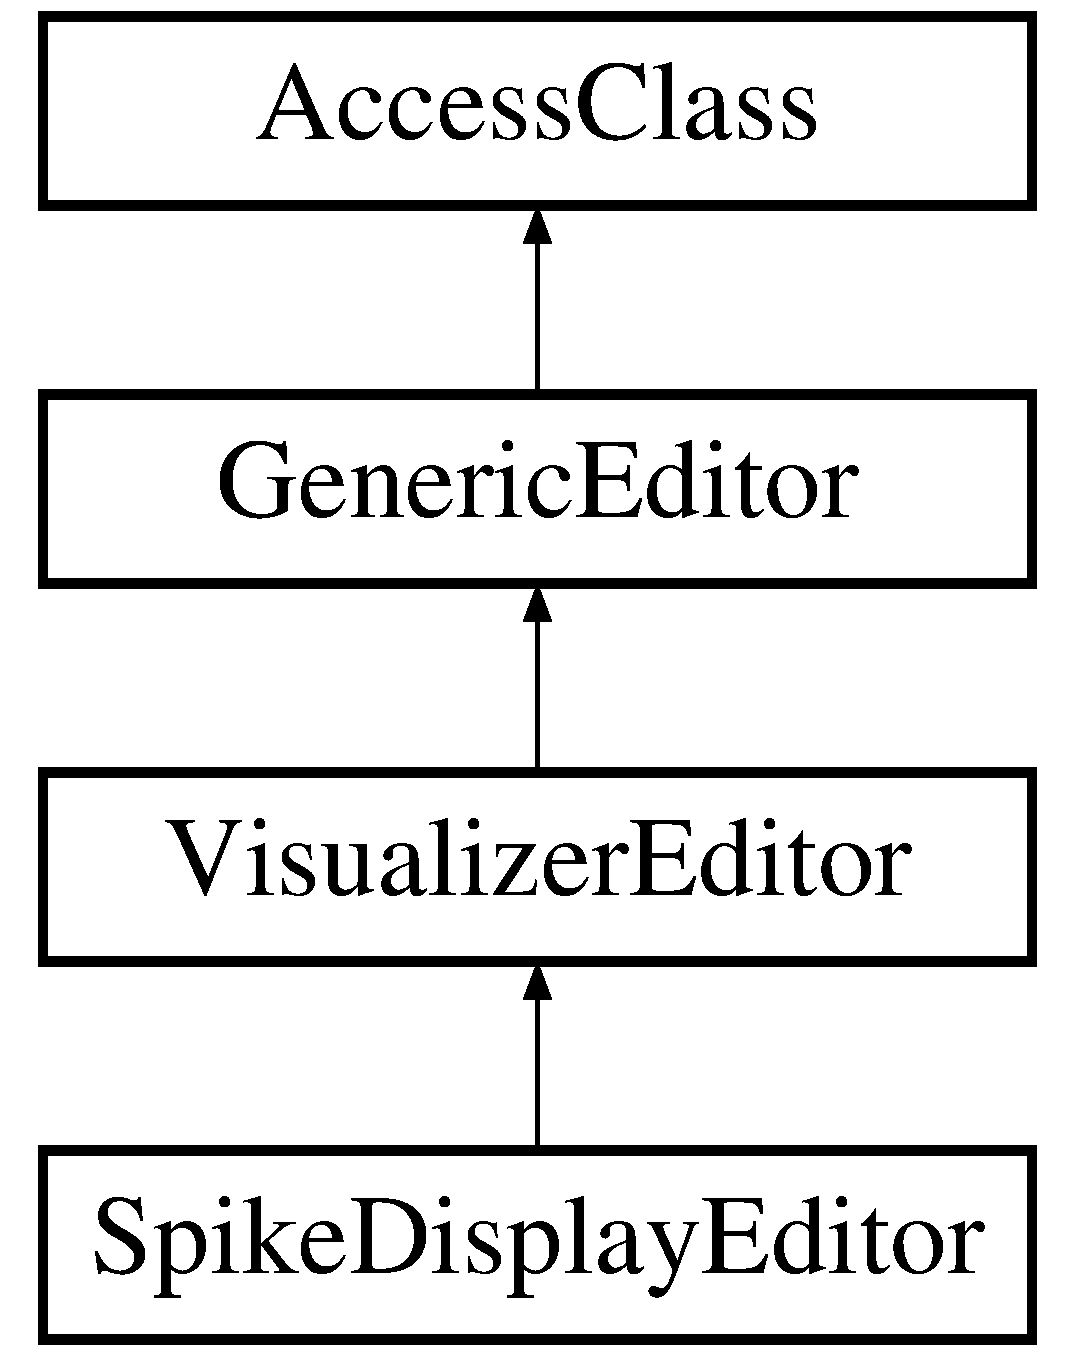
\includegraphics[height=4.000000cm]{classSpikeDisplayEditor}
\end{center}
\end{figure}
\subsection*{Public Member Functions}
\begin{DoxyCompactItemize}
\item 
\hypertarget{classSpikeDisplayEditor_ac983964da6dcf139ffaaa93473d8bc58}{{\bfseries Spike\-Display\-Editor} (\hyperlink{classGenericProcessor}{Generic\-Processor} $\ast$)}\label{classSpikeDisplayEditor_ac983964da6dcf139ffaaa93473d8bc58}

\item 
\hypertarget{classSpikeDisplayEditor_a5c622a46511053389820d631f2dcc88d}{void {\bfseries button\-Callback} (Button $\ast$button)}\label{classSpikeDisplayEditor_a5c622a46511053389820d631f2dcc88d}

\item 
\hypertarget{classSpikeDisplayEditor_a050a9b899e6028b6ec87b0b2a97d1a97}{\hyperlink{classVisualizer}{Visualizer} $\ast$ {\bfseries create\-New\-Canvas} ()}\label{classSpikeDisplayEditor_a050a9b899e6028b6ec87b0b2a97d1a97}

\end{DoxyCompactItemize}
\subsection*{Private Member Functions}
\begin{DoxyCompactItemize}
\item 
\hypertarget{classSpikeDisplayEditor_a2be7b29f480be05058f1c214a4458a0b}{void {\bfseries initialize\-Buttons} ()}\label{classSpikeDisplayEditor_a2be7b29f480be05058f1c214a4458a0b}

\item 
\hypertarget{classSpikeDisplayEditor_acfc32c99c09564b8885cb882638a677f}{{\bfseries J\-U\-C\-E\-\_\-\-D\-E\-C\-L\-A\-R\-E\-\_\-\-N\-O\-N\-\_\-\-C\-O\-P\-Y\-A\-B\-L\-E\-\_\-\-W\-I\-T\-H\-\_\-\-L\-E\-A\-K\-\_\-\-D\-E\-T\-E\-C\-T\-O\-R} (\hyperlink{classSpikeDisplayEditor}{Spike\-Display\-Editor})}\label{classSpikeDisplayEditor_acfc32c99c09564b8885cb882638a677f}

\end{DoxyCompactItemize}
\subsection*{Private Attributes}
\begin{DoxyCompactItemize}
\item 
\hypertarget{classSpikeDisplayEditor_a984755ff3624a85c5d31c2350080d700}{\hyperlink{classUtilityButton}{Utility\-Button} $\ast$ {\bfseries pan\-Up\-Btn}}\label{classSpikeDisplayEditor_a984755ff3624a85c5d31c2350080d700}

\item 
\hypertarget{classSpikeDisplayEditor_afee4c5306fdaf4cb3548af17f4d23786}{\hyperlink{classUtilityButton}{Utility\-Button} $\ast$ {\bfseries pan\-Down\-Btn}}\label{classSpikeDisplayEditor_afee4c5306fdaf4cb3548af17f4d23786}

\item 
\hypertarget{classSpikeDisplayEditor_acf23b32593c1379f58a2e110baa91ed8}{\hyperlink{classUtilityButton}{Utility\-Button} $\ast$ {\bfseries zoom\-In\-Btn}}\label{classSpikeDisplayEditor_acf23b32593c1379f58a2e110baa91ed8}

\item 
\hypertarget{classSpikeDisplayEditor_ab303083b47b70e8ecfbd3a44f2106be4}{\hyperlink{classUtilityButton}{Utility\-Button} $\ast$ {\bfseries zoom\-Out\-Btn}}\label{classSpikeDisplayEditor_ab303083b47b70e8ecfbd3a44f2106be4}

\item 
\hypertarget{classSpikeDisplayEditor_a8f6876e9e2c2eca307ec71bd756f8c79}{\hyperlink{classUtilityButton}{Utility\-Button} $\ast$ {\bfseries clear\-Btn}}\label{classSpikeDisplayEditor_a8f6876e9e2c2eca307ec71bd756f8c79}

\item 
\hypertarget{classSpikeDisplayEditor_abf4ea3ab5df0a76c1f6f76751289da00}{\hyperlink{classUtilityButton}{Utility\-Button} $\ast$ {\bfseries save\-Img\-Btn}}\label{classSpikeDisplayEditor_abf4ea3ab5df0a76c1f6f76751289da00}

\item 
\hypertarget{classSpikeDisplayEditor_a1a540bb1adbed3f96051a1370c1d8221}{Label $\ast$ {\bfseries pan\-Label}}\label{classSpikeDisplayEditor_a1a540bb1adbed3f96051a1370c1d8221}

\item 
\hypertarget{classSpikeDisplayEditor_ad465a9ce6db3d09a5b94bccd2af1fa8e}{Label $\ast$ {\bfseries zoom\-Label}}\label{classSpikeDisplayEditor_ad465a9ce6db3d09a5b94bccd2af1fa8e}

\item 
\hypertarget{classSpikeDisplayEditor_aaf44191f75ab94175249b6e844c63bce}{\hyperlink{classUtilityButton}{Utility\-Button} $\ast$ {\bfseries all\-Sub\-Chans\-Btn}}\label{classSpikeDisplayEditor_aaf44191f75ab94175249b6e844c63bce}

\item 
\hypertarget{classSpikeDisplayEditor_a5c008c4e2d3b39d96046f1e9c0784802}{int {\bfseries n\-Sub\-Channels}}\label{classSpikeDisplayEditor_a5c008c4e2d3b39d96046f1e9c0784802}

\item 
\hypertarget{classSpikeDisplayEditor_a3291774d897476b171ebbfcd76101520}{Label $\ast$ {\bfseries sub\-Chan\-Label}}\label{classSpikeDisplayEditor_a3291774d897476b171ebbfcd76101520}

\item 
\hypertarget{classSpikeDisplayEditor_af49e74e3dec861024f2c501218c5d1c9}{\hyperlink{classUtilityButton}{Utility\-Button} $\ast$ {\bfseries sub\-Chan\-Btn} \mbox{[}M\-A\-X\-\_\-\-N\-\_\-\-S\-U\-B\-\_\-\-C\-H\-A\-N\mbox{]}}\label{classSpikeDisplayEditor_af49e74e3dec861024f2c501218c5d1c9}

\item 
\hypertarget{classSpikeDisplayEditor_ae7e6e3e7c3a263144f1981cb6bd090db}{bool {\bfseries sub\-Chan\-Selected} \mbox{[}M\-A\-X\-\_\-\-N\-\_\-\-S\-U\-B\-\_\-\-C\-H\-A\-N\mbox{]}}\label{classSpikeDisplayEditor_ae7e6e3e7c3a263144f1981cb6bd090db}

\end{DoxyCompactItemize}
\subsection*{Additional Inherited Members}


The documentation for this class was generated from the following file\-:\begin{DoxyCompactItemize}
\item 
Processors/\-Editors/Spike\-Display\-Editor.\-h\end{DoxyCompactItemize}

\hypertarget{classSpikeDisplayNode}{\section{Spike\-Display\-Node Class Reference}
\label{classSpikeDisplayNode}\index{Spike\-Display\-Node@{Spike\-Display\-Node}}
}
Inheritance diagram for Spike\-Display\-Node\-:\begin{figure}[H]
\begin{center}
\leavevmode
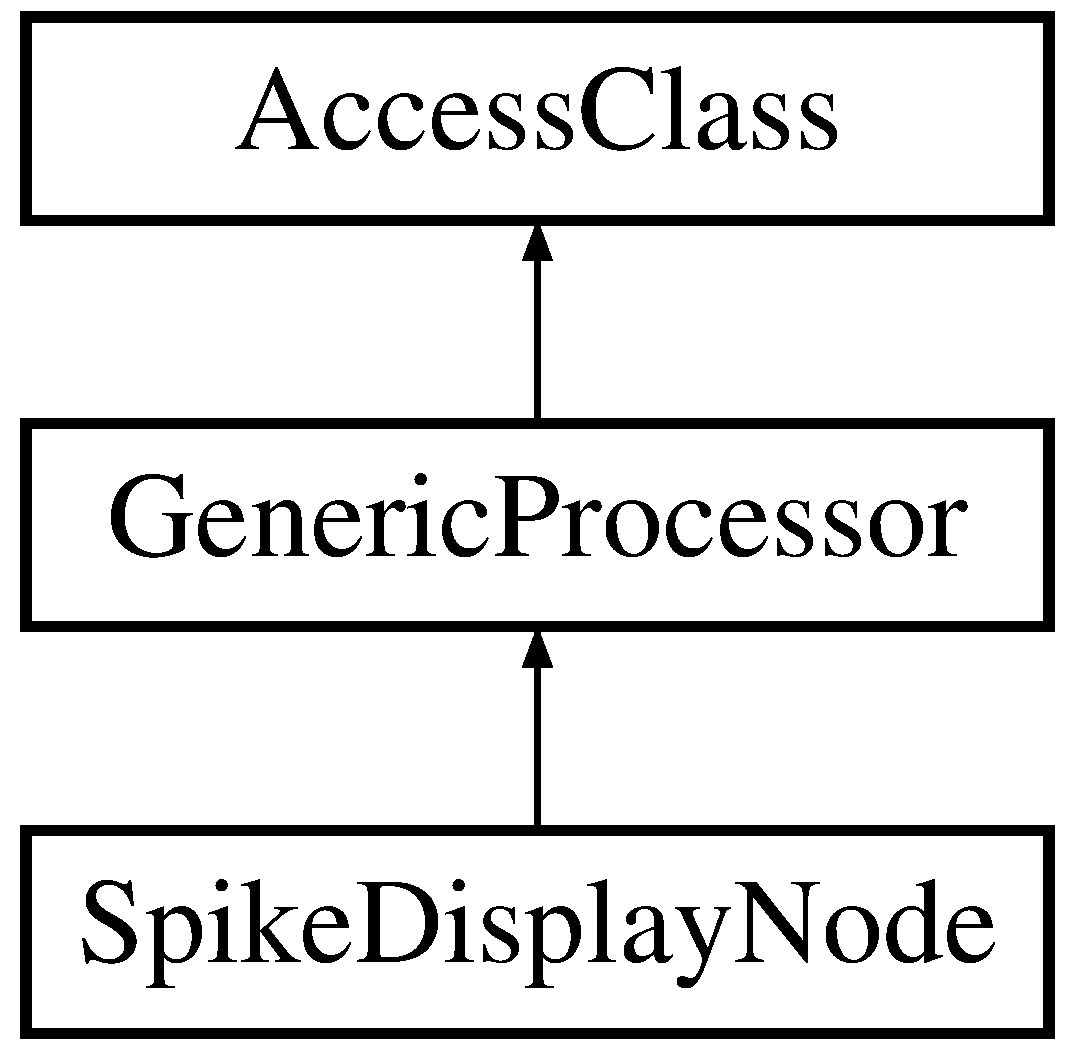
\includegraphics[height=3.000000cm]{classSpikeDisplayNode}
\end{center}
\end{figure}
\subsection*{Public Member Functions}
\begin{DoxyCompactItemize}
\item 
\hypertarget{classSpikeDisplayNode_a313aadc4cf4cde9bd4ef08c9119b9cf9}{Audio\-Processor\-Editor $\ast$ {\bfseries create\-Editor} ()}\label{classSpikeDisplayNode_a313aadc4cf4cde9bd4ef08c9119b9cf9}

\item 
\hypertarget{classSpikeDisplayNode_a2daedb6bd54b65b5b3bbf1b507d7d568}{bool {\bfseries is\-Sink} ()}\label{classSpikeDisplayNode_a2daedb6bd54b65b5b3bbf1b507d7d568}

\item 
\hypertarget{classSpikeDisplayNode_a5c6d9afd49e85f383ec5631d232dca76}{void {\bfseries process} (Audio\-Sample\-Buffer \&buffer, Midi\-Buffer \&midi\-Messages, int \&n\-Samples)}\label{classSpikeDisplayNode_a5c6d9afd49e85f383ec5631d232dca76}

\item 
\hypertarget{classSpikeDisplayNode_a000a21d39870567e6b95f0676fcd2d51}{void {\bfseries set\-Parameter} (int, float)}\label{classSpikeDisplayNode_a000a21d39870567e6b95f0676fcd2d51}

\item 
\hypertarget{classSpikeDisplayNode_a5aeb76922e1f99d873ddf9d0b39b261e}{void {\bfseries handle\-Event} (int, Midi\-Message \&)}\label{classSpikeDisplayNode_a5aeb76922e1f99d873ddf9d0b39b261e}

\item 
\hypertarget{classSpikeDisplayNode_a27467b2a989ce2e83153d578a5567dd7}{bool {\bfseries enable} ()}\label{classSpikeDisplayNode_a27467b2a989ce2e83153d578a5567dd7}

\item 
\hypertarget{classSpikeDisplayNode_a7d360430be47c72f14a8a776b945dd1a}{bool {\bfseries disable} ()}\label{classSpikeDisplayNode_a7d360430be47c72f14a8a776b945dd1a}

\item 
\hypertarget{classSpikeDisplayNode_a1090bac27990b984f670c8935c17cc97}{Midi\-Buffer $\ast$ {\bfseries get\-Spike\-Buffer\-Address} ()}\label{classSpikeDisplayNode_a1090bac27990b984f670c8935c17cc97}

\item 
\hypertarget{classSpikeDisplayNode_a85908f865f1692bacf36df869170616c}{int {\bfseries get\-Number\-Of\-Channels\-For\-Electrode} (int i)}\label{classSpikeDisplayNode_a85908f865f1692bacf36df869170616c}

\item 
\hypertarget{classSpikeDisplayNode_a51acdbe4570fd6f65dd361f2ba7cff26}{int {\bfseries get\-Num\-Electrodes} ()}\label{classSpikeDisplayNode_a51acdbe4570fd6f65dd361f2ba7cff26}

\item 
\hypertarget{classSpikeDisplayNode_a53dc19ffc860d58dc5bc7ac1f030909d}{bool {\bfseries get\-Next\-Spike} (\hyperlink{structSpikeObject}{Spike\-Object} $\ast$spike)}\label{classSpikeDisplayNode_a53dc19ffc860d58dc5bc7ac1f030909d}

\end{DoxyCompactItemize}
\subsection*{Private Member Functions}
\begin{DoxyCompactItemize}
\item 
\hypertarget{classSpikeDisplayNode_a3777bdf9658cff6e3afa614c4dac42e0}{{\bfseries J\-U\-C\-E\-\_\-\-D\-E\-C\-L\-A\-R\-E\-\_\-\-N\-O\-N\-\_\-\-C\-O\-P\-Y\-A\-B\-L\-E\-\_\-\-W\-I\-T\-H\-\_\-\-L\-E\-A\-K\-\_\-\-D\-E\-T\-E\-C\-T\-O\-R} (\hyperlink{classSpikeDisplayNode}{Spike\-Display\-Node})}\label{classSpikeDisplayNode_a3777bdf9658cff6e3afa614c4dac42e0}

\end{DoxyCompactItemize}
\subsection*{Private Attributes}
\begin{DoxyCompactItemize}
\item 
\hypertarget{classSpikeDisplayNode_a7ddbfc9ca3815b4315bb69b72c3fa177}{int {\bfseries number\-Of\-Sources}}\label{classSpikeDisplayNode_a7ddbfc9ca3815b4315bb69b72c3fa177}

\item 
\hypertarget{classSpikeDisplayNode_aa5890dded2c29e97d9ba24281d9abc76}{Scoped\-Pointer$<$ Midi\-Buffer $>$ {\bfseries event\-Buffer}}\label{classSpikeDisplayNode_aa5890dded2c29e97d9ba24281d9abc76}

\item 
\hypertarget{classSpikeDisplayNode_a80df931484f4fa03a1a1a1a8863e3638}{int {\bfseries buffer\-Size}}\label{classSpikeDisplayNode_a80df931484f4fa03a1a1a1a8863e3638}

\end{DoxyCompactItemize}
\subsection*{Additional Inherited Members}


The documentation for this class was generated from the following file\-:\begin{DoxyCompactItemize}
\item 
Processors/Spike\-Display\-Node.\-h\end{DoxyCompactItemize}

\hypertarget{structSpikeObject}{\section{Spike\-Object Struct Reference}
\label{structSpikeObject}\index{Spike\-Object@{Spike\-Object}}
}
\subsection*{Public Attributes}
\begin{DoxyCompactItemize}
\item 
\hypertarget{structSpikeObject_a89a9d28a3f76e004c5434ab87a13f6ce}{uint8\-\_\-t {\bfseries event\-Type}}\label{structSpikeObject_a89a9d28a3f76e004c5434ab87a13f6ce}

\item 
\hypertarget{structSpikeObject_ad9b485d97938e01e1e8ed5044d26aaf5}{uint64\-\_\-t {\bfseries timestamp}}\label{structSpikeObject_ad9b485d97938e01e1e8ed5044d26aaf5}

\item 
\hypertarget{structSpikeObject_ad82d2c52cd9262794947807cc70f0bc8}{uint16\-\_\-t {\bfseries source}}\label{structSpikeObject_ad82d2c52cd9262794947807cc70f0bc8}

\item 
\hypertarget{structSpikeObject_a126c96ef75bce81f86e45ed6559f16f0}{uint16\-\_\-t {\bfseries n\-Channels}}\label{structSpikeObject_a126c96ef75bce81f86e45ed6559f16f0}

\item 
\hypertarget{structSpikeObject_addde0b7ca60cad4b48e8def822eee034}{uint16\-\_\-t {\bfseries n\-Samples}}\label{structSpikeObject_addde0b7ca60cad4b48e8def822eee034}

\item 
\hypertarget{structSpikeObject_ab64109049bbe27ddbf44fa7441698103}{uint16\-\_\-t {\bfseries data} \mbox{[}M\-A\-X\-\_\-\-N\-U\-M\-B\-E\-R\-\_\-\-O\-F\-\_\-\-S\-P\-I\-K\-E\-\_\-\-C\-H\-A\-N\-N\-E\-L\-S $\ast$M\-A\-X\-\_\-\-N\-U\-M\-B\-E\-R\-\_\-\-O\-F\-\_\-\-S\-P\-I\-K\-E\-\_\-\-C\-H\-A\-N\-N\-E\-L\-\_\-\-S\-A\-M\-P\-L\-E\-S\mbox{]}}\label{structSpikeObject_ab64109049bbe27ddbf44fa7441698103}

\item 
\hypertarget{structSpikeObject_aeb26d8b44806e5d80ee785e28db122ce}{uint16\-\_\-t {\bfseries gain} \mbox{[}M\-A\-X\-\_\-\-N\-U\-M\-B\-E\-R\-\_\-\-O\-F\-\_\-\-S\-P\-I\-K\-E\-\_\-\-C\-H\-A\-N\-N\-E\-L\-S\mbox{]}}\label{structSpikeObject_aeb26d8b44806e5d80ee785e28db122ce}

\item 
\hypertarget{structSpikeObject_aa3b4cec4bcc9b1e1ad0f50d8babead63}{uint16\-\_\-t {\bfseries threshold} \mbox{[}M\-A\-X\-\_\-\-N\-U\-M\-B\-E\-R\-\_\-\-O\-F\-\_\-\-S\-P\-I\-K\-E\-\_\-\-C\-H\-A\-N\-N\-E\-L\-S\mbox{]}}\label{structSpikeObject_aa3b4cec4bcc9b1e1ad0f50d8babead63}

\end{DoxyCompactItemize}


The documentation for this struct was generated from the following file\-:\begin{DoxyCompactItemize}
\item 
Processors/\-Visualization/Spike\-Object.\-h\end{DoxyCompactItemize}

\hypertarget{classSplitter}{\section{Splitter Class Reference}
\label{classSplitter}\index{Splitter@{Splitter}}
}


{\ttfamily \#include $<$Splitter.\-h$>$}

Inheritance diagram for Splitter\-:\begin{figure}[H]
\begin{center}
\leavevmode
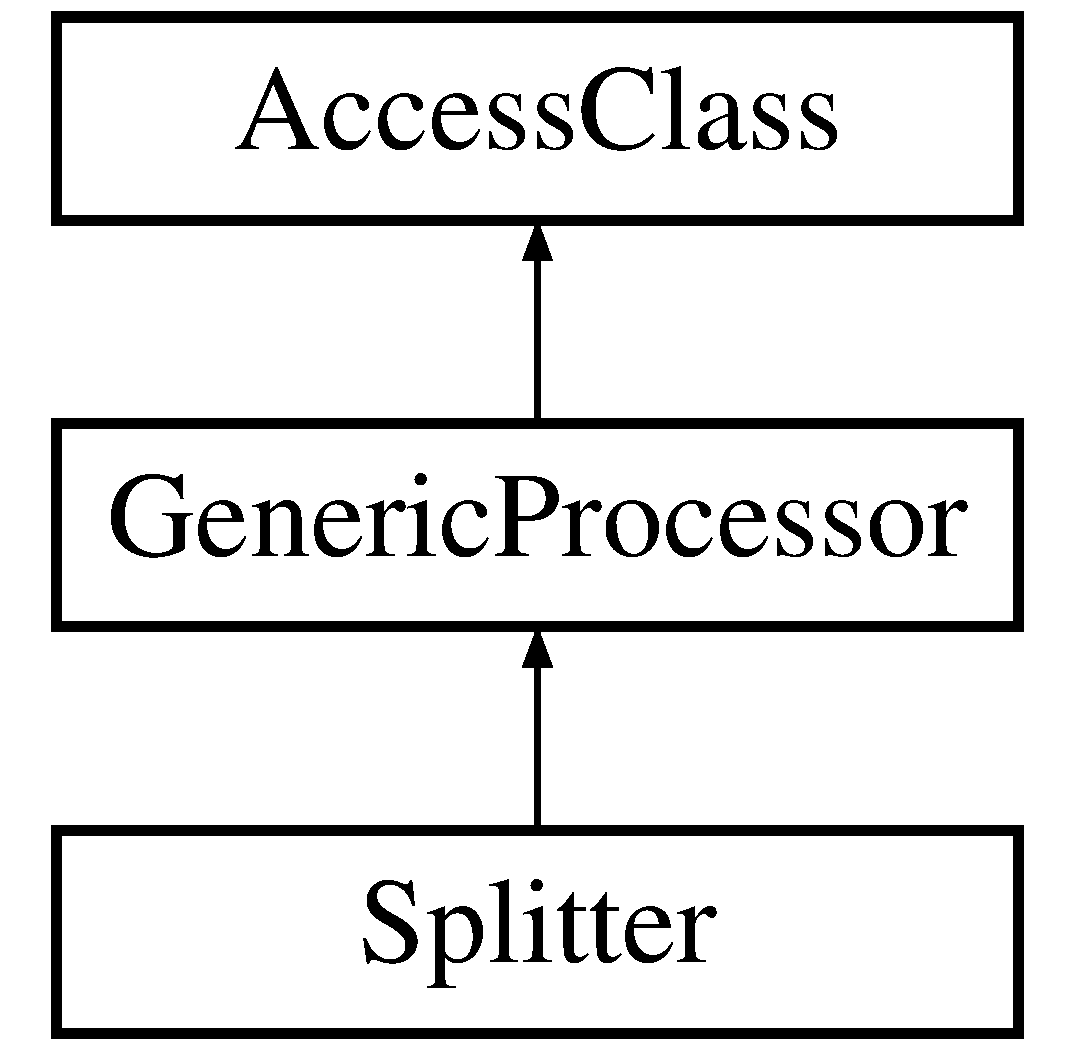
\includegraphics[height=3.000000cm]{classSplitter}
\end{center}
\end{figure}
\subsection*{Public Member Functions}
\begin{DoxyCompactItemize}
\item 
\hypertarget{classSplitter_a1efaec57eeafba93724921f8de2fc296}{Audio\-Processor\-Editor $\ast$ {\bfseries create\-Editor} ()}\label{classSplitter_a1efaec57eeafba93724921f8de2fc296}

\item 
\hypertarget{classSplitter_a0ad1211a06e6a6317d89eb6257d178d3}{void {\bfseries process} (Audio\-Sample\-Buffer \&buffer, Midi\-Buffer \&midi\-Messages, int \&n\-Samples)}\label{classSplitter_a0ad1211a06e6a6317d89eb6257d178d3}

\item 
\hypertarget{classSplitter_ac63efb523b23518f2417b9e983affa31}{bool {\bfseries is\-Splitter} ()}\label{classSplitter_ac63efb523b23518f2417b9e983affa31}

\item 
\hypertarget{classSplitter_a760a6d86203940549bc096e2fa224be3}{void {\bfseries switch\-I\-O} (int)}\label{classSplitter_a760a6d86203940549bc096e2fa224be3}

\item 
\hypertarget{classSplitter_ac1b94259cfe2943f55315dd523f20307}{void {\bfseries switch\-I\-O} ()}\label{classSplitter_ac1b94259cfe2943f55315dd523f20307}

\item 
\hypertarget{classSplitter_ae11524d844f439fc3a101cc7de534c1b}{void {\bfseries set\-Splitter\-Dest\-Node} (\hyperlink{classGenericProcessor}{Generic\-Processor} $\ast$dn)}\label{classSplitter_ae11524d844f439fc3a101cc7de534c1b}

\item 
\hypertarget{classSplitter_a51f9501f7601773bfe5b7f57958f4135}{void {\bfseries set\-Path\-To\-Processor} (\hyperlink{classGenericProcessor}{Generic\-Processor} $\ast$processor)}\label{classSplitter_a51f9501f7601773bfe5b7f57958f4135}

\item 
\hypertarget{classSplitter_a27e4746563139cce811ddd528fe405b8}{int {\bfseries get\-Path} ()}\label{classSplitter_a27e4746563139cce811ddd528fe405b8}

\end{DoxyCompactItemize}
\subsection*{Private Member Functions}
\begin{DoxyCompactItemize}
\item 
\hypertarget{classSplitter_ae2ec58c73fc3c0254422527054e8923b}{{\bfseries J\-U\-C\-E\-\_\-\-D\-E\-C\-L\-A\-R\-E\-\_\-\-N\-O\-N\-\_\-\-C\-O\-P\-Y\-A\-B\-L\-E\-\_\-\-W\-I\-T\-H\-\_\-\-L\-E\-A\-K\-\_\-\-D\-E\-T\-E\-C\-T\-O\-R} (\hyperlink{classSplitter}{Splitter})}\label{classSplitter_ae2ec58c73fc3c0254422527054e8923b}

\end{DoxyCompactItemize}
\subsection*{Private Attributes}
\begin{DoxyCompactItemize}
\item 
\hypertarget{classSplitter_a612aa88eafc53648ea6d2f3ef9ce25f7}{\hyperlink{classGenericProcessor}{Generic\-Processor} $\ast$ {\bfseries dest\-Node\-A}}\label{classSplitter_a612aa88eafc53648ea6d2f3ef9ce25f7}

\item 
\hypertarget{classSplitter_a02597536b91e85671fd16edcb8cc16d7}{\hyperlink{classGenericProcessor}{Generic\-Processor} $\ast$ {\bfseries dest\-Node\-B}}\label{classSplitter_a02597536b91e85671fd16edcb8cc16d7}

\item 
\hypertarget{classSplitter_a80a5b64b670adcc887b05f2b3e5f27bf}{int {\bfseries active\-Path}}\label{classSplitter_a80a5b64b670adcc887b05f2b3e5f27bf}

\end{DoxyCompactItemize}
\subsection*{Additional Inherited Members}


\subsection{Detailed Description}
Allows the user to split the signal chain.

\begin{DoxySeeAlso}{See also}
\hyperlink{classGenericProcessor}{Generic\-Processor}, \hyperlink{classProcessorGraph}{Processor\-Graph} 
\end{DoxySeeAlso}


The documentation for this class was generated from the following file\-:\begin{DoxyCompactItemize}
\item 
Processors/\-Utilities/Splitter.\-h\end{DoxyCompactItemize}

\hypertarget{classSplitterEditor}{\section{Splitter\-Editor Class Reference}
\label{classSplitterEditor}\index{Splitter\-Editor@{Splitter\-Editor}}
}
Inheritance diagram for Splitter\-Editor\-:\begin{figure}[H]
\begin{center}
\leavevmode
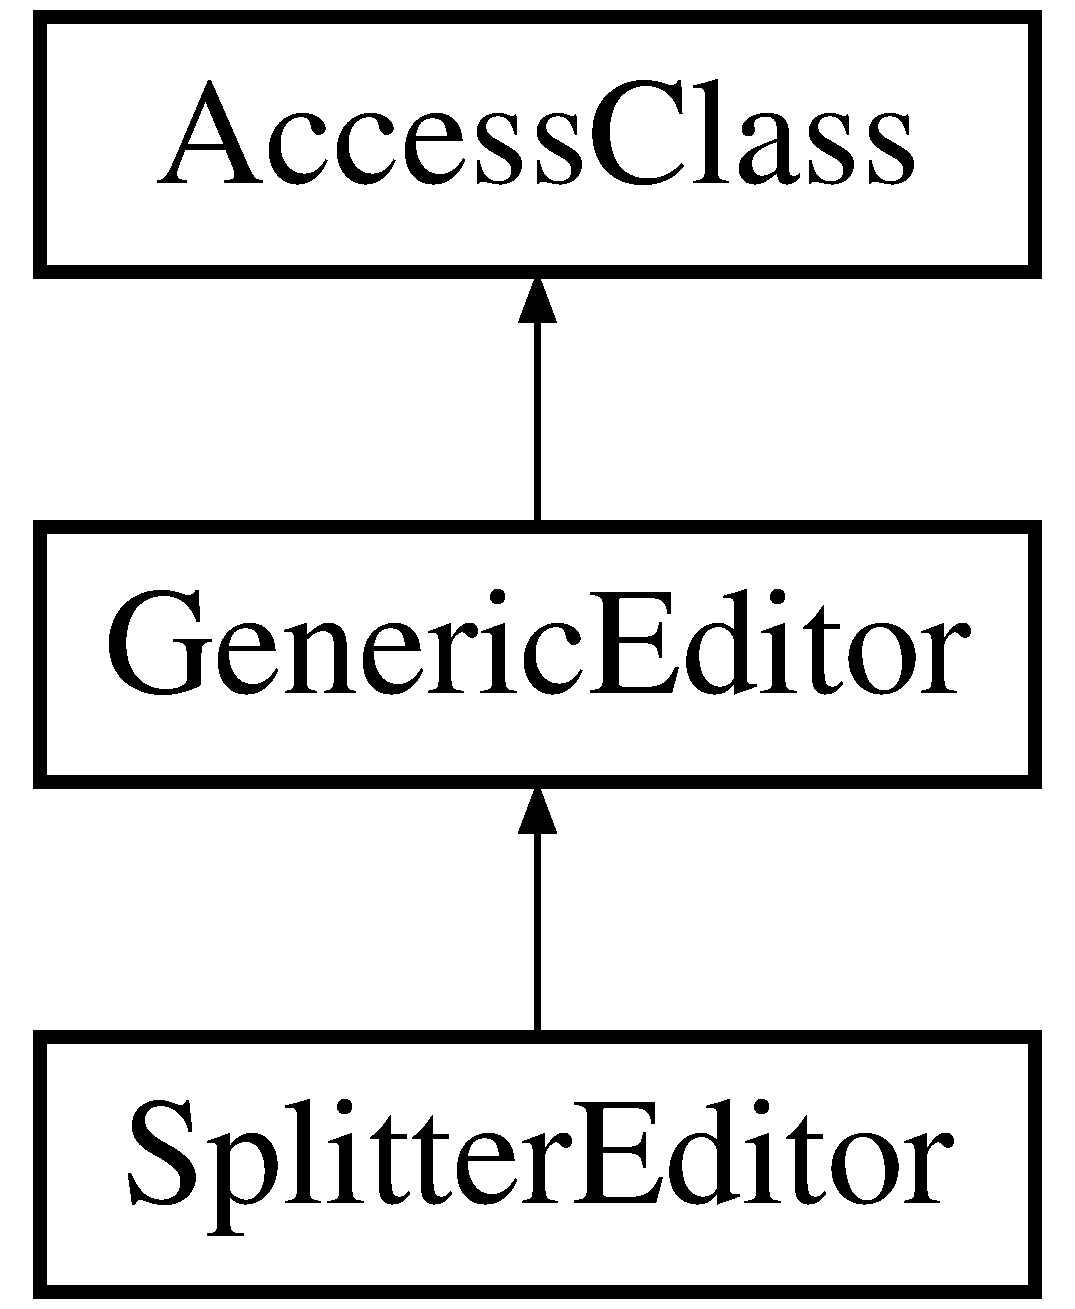
\includegraphics[height=3.000000cm]{classSplitterEditor}
\end{center}
\end{figure}
\subsection*{Public Member Functions}
\begin{DoxyCompactItemize}
\item 
\hypertarget{classSplitterEditor_aaf755e6bc0447d9660365a5fbd40f052}{{\bfseries Splitter\-Editor} (\hyperlink{classGenericProcessor}{Generic\-Processor} $\ast$parent\-Node)}\label{classSplitterEditor_aaf755e6bc0447d9660365a5fbd40f052}

\item 
\hypertarget{classSplitterEditor_a8965e72d47eacbb196b78c19ff441526}{void {\bfseries button\-Event} (Button $\ast$button)}\label{classSplitterEditor_a8965e72d47eacbb196b78c19ff441526}

\item 
\hypertarget{classSplitterEditor_a562704e5e9dd487175881e18820b958f}{void {\bfseries switch\-Dest} (int)}\label{classSplitterEditor_a562704e5e9dd487175881e18820b958f}

\item 
\hypertarget{classSplitterEditor_a55deac87232a7e7d15b0c0d3fe4d8256}{void {\bfseries switch\-Dest} ()}\label{classSplitterEditor_a55deac87232a7e7d15b0c0d3fe4d8256}

\item 
\hypertarget{classSplitterEditor_a192851e62390ad3aeb5fe2e98ddb50f3}{void {\bfseries switch\-I\-O} (int i)}\label{classSplitterEditor_a192851e62390ad3aeb5fe2e98ddb50f3}

\end{DoxyCompactItemize}
\subsection*{Private Member Functions}
\begin{DoxyCompactItemize}
\item 
\hypertarget{classSplitterEditor_a0bd85c437886569153ddffee21f0affb}{{\bfseries J\-U\-C\-E\-\_\-\-D\-E\-C\-L\-A\-R\-E\-\_\-\-N\-O\-N\-\_\-\-C\-O\-P\-Y\-A\-B\-L\-E\-\_\-\-W\-I\-T\-H\-\_\-\-L\-E\-A\-K\-\_\-\-D\-E\-T\-E\-C\-T\-O\-R} (\hyperlink{classSplitterEditor}{Splitter\-Editor})}\label{classSplitterEditor_a0bd85c437886569153ddffee21f0affb}

\end{DoxyCompactItemize}
\subsection*{Private Attributes}
\begin{DoxyCompactItemize}
\item 
\hypertarget{classSplitterEditor_a11851bcb7d1c134a663d657e2924b921}{Image\-Button $\ast$ {\bfseries pipeline\-Selector\-A}}\label{classSplitterEditor_a11851bcb7d1c134a663d657e2924b921}

\item 
\hypertarget{classSplitterEditor_a21e5a1c5bde20979a4c8f779598e8cb0}{Image\-Button $\ast$ {\bfseries pipeline\-Selector\-B}}\label{classSplitterEditor_a21e5a1c5bde20979a4c8f779598e8cb0}

\end{DoxyCompactItemize}
\subsection*{Additional Inherited Members}


The documentation for this class was generated from the following file\-:\begin{DoxyCompactItemize}
\item 
Processors/\-Editors/Splitter\-Editor.\-h\end{DoxyCompactItemize}

\hypertarget{classStereotrodePlot}{\section{Stereotrode\-Plot Class Reference}
\label{classStereotrodePlot}\index{Stereotrode\-Plot@{Stereotrode\-Plot}}
}
Inheritance diagram for Stereotrode\-Plot\-:\begin{figure}[H]
\begin{center}
\leavevmode
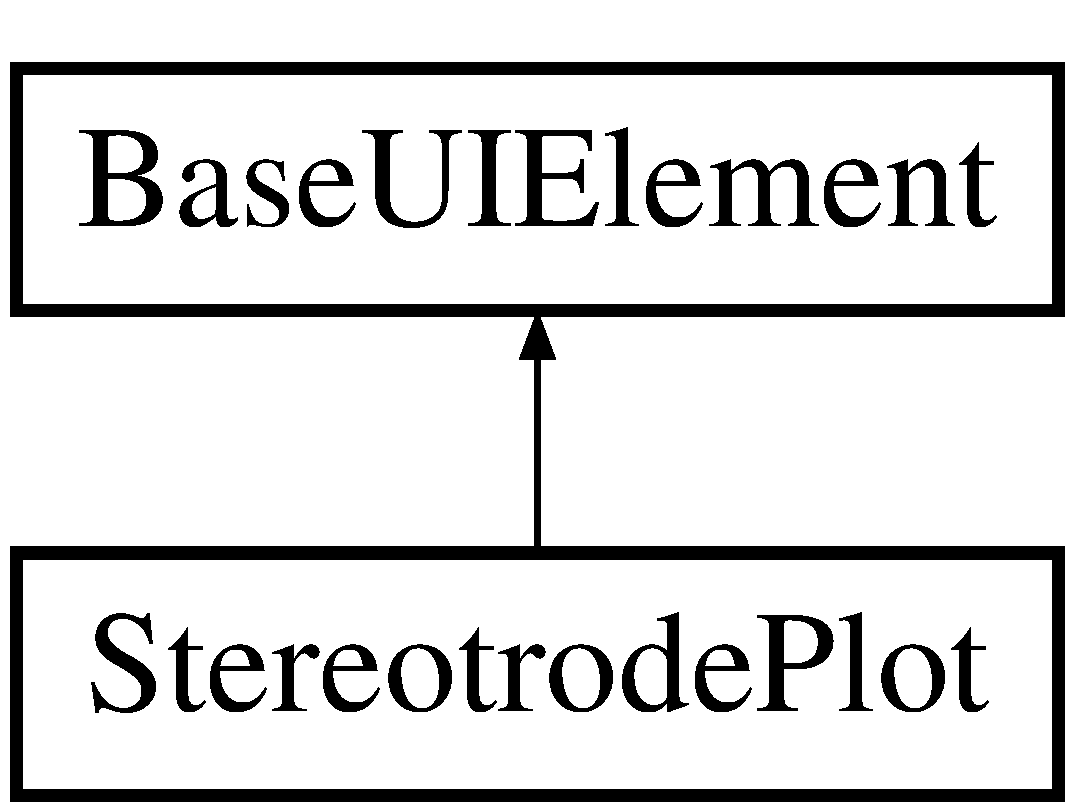
\includegraphics[height=2.000000cm]{classStereotrodePlot}
\end{center}
\end{figure}
\subsection*{Public Member Functions}
\begin{DoxyCompactItemize}
\item 
\hypertarget{classStereotrodePlot_a28f0041e93010dd5dad4c8e51a26cc6f}{{\bfseries Stereotrode\-Plot} (int x, int y, int w, int h)}\label{classStereotrodePlot_a28f0041e93010dd5dad4c8e51a26cc6f}

\item 
\hypertarget{classStereotrodePlot_ad5a5e70eecfddf9dd3d3de15ef76d792}{void {\bfseries init\-Axes} ()}\label{classStereotrodePlot_ad5a5e70eecfddf9dd3d3de15ef76d792}

\item 
\hypertarget{classStereotrodePlot_a0b3dd83ece8eb6e31f6e0311cf23da7e}{void {\bfseries redraw} ()}\label{classStereotrodePlot_a0b3dd83ece8eb6e31f6e0311cf23da7e}

\item 
\hypertarget{classStereotrodePlot_aad88b7592b8f3c44762ed37cf3751b90}{void {\bfseries set\-Enabled} (bool enabled)}\label{classStereotrodePlot_aad88b7592b8f3c44762ed37cf3751b90}

\item 
\hypertarget{classStereotrodePlot_a0f9acb82119a690dd7bc899af934ad99}{bool {\bfseries get\-Enabled} ()}\label{classStereotrodePlot_a0f9acb82119a690dd7bc899af934ad99}

\item 
\hypertarget{classStereotrodePlot_ade3c280e004b7fcb399d5e0b4da71c2f}{void {\bfseries set\-Position} (int, int, double, double)}\label{classStereotrodePlot_ade3c280e004b7fcb399d5e0b4da71c2f}

\item 
\hypertarget{classStereotrodePlot_ab459fad08156637d5e7f81e68d4f6e2b}{void {\bfseries get\-Preferred\-Dimensions} (double $\ast$, double $\ast$)}\label{classStereotrodePlot_ab459fad08156637d5e7f81e68d4f6e2b}

\item 
\hypertarget{classStereotrodePlot_a08ac5f1a8cb909590ac813f7b2cbb3bc}{int {\bfseries get\-Number\-Of\-Axes} ()}\label{classStereotrodePlot_a08ac5f1a8cb909590ac813f7b2cbb3bc}

\item 
\hypertarget{classStereotrodePlot_add199a472990150407c924c1f5f98a3d}{void {\bfseries mouse\-Down} (int x, int y)}\label{classStereotrodePlot_add199a472990150407c924c1f5f98a3d}

\item 
\hypertarget{classStereotrodePlot_aa815cd74cd2e69bd38aea6652292b9cc}{void {\bfseries mouse\-Drag\-X} (int dx, bool shift, bool ctr)}\label{classStereotrodePlot_aa815cd74cd2e69bd38aea6652292b9cc}

\item 
\hypertarget{classStereotrodePlot_ae7617aa26fbbcbe15ed801a27730976d}{void {\bfseries mouse\-Drag\-Y} (int dy, bool shift, bool ctr)}\label{classStereotrodePlot_ae7617aa26fbbcbe15ed801a27730976d}

\item 
\hypertarget{classStereotrodePlot_affd802a81737b9014b09d796ae373942}{bool {\bfseries process\-Key\-Event} (\hyperlink{structSimpleKeyEvent}{Simple\-Key\-Event} k)}\label{classStereotrodePlot_affd802a81737b9014b09d796ae373942}

\item 
\hypertarget{classStereotrodePlot_a9d197c94a09087ec058724e1b1854017}{void {\bfseries process\-Spike\-Object} (\hyperlink{structSpikeObject}{Spike\-Object} s)}\label{classStereotrodePlot_a9d197c94a09087ec058724e1b1854017}

\item 
\hypertarget{classStereotrodePlot_a59d2e1d5dc55ca25b34fc0da30187707}{void {\bfseries clear} ()}\label{classStereotrodePlot_a59d2e1d5dc55ca25b34fc0da30187707}

\item 
\hypertarget{classStereotrodePlot_a57903b22d7be7c20d26b1ca996a6e192}{void {\bfseries zoom} (int, bool)}\label{classStereotrodePlot_a57903b22d7be7c20d26b1ca996a6e192}

\item 
\hypertarget{classStereotrodePlot_ac9a104b9bed4aa493e2a65a68e67a600}{void {\bfseries pan} (int, bool)}\label{classStereotrodePlot_ac9a104b9bed4aa493e2a65a68e67a600}

\end{DoxyCompactItemize}
\subsection*{Private Member Functions}
\begin{DoxyCompactItemize}
\item 
\hypertarget{classStereotrodePlot_a75dd01ab7ba238a744a0b137bbf78002}{void {\bfseries init\-Limits} ()}\label{classStereotrodePlot_a75dd01ab7ba238a744a0b137bbf78002}

\item 
\hypertarget{classStereotrodePlot_a28b4fccd31b9adbf449449a8ead1e2a3}{void {\bfseries set\-Limits\-On\-Axes} ()}\label{classStereotrodePlot_a28b4fccd31b9adbf449449a8ead1e2a3}

\end{DoxyCompactItemize}
\subsection*{Private Attributes}
\begin{DoxyCompactItemize}
\item 
\hypertarget{classStereotrodePlot_a78a80fe4052fd96057d142dad3bcb29a}{bool {\bfseries enabled}}\label{classStereotrodePlot_a78a80fe4052fd96057d142dad3bcb29a}

\item 
\hypertarget{classStereotrodePlot_a7178827c495da19c66ed6cc6b5e6ec45}{bool {\bfseries limits\-Changed}}\label{classStereotrodePlot_a7178827c495da19c66ed6cc6b5e6ec45}

\item 
\hypertarget{classStereotrodePlot_a83eb2f6280de73854c2e0893595e741e}{double {\bfseries limits} \mbox{[}2\mbox{]}\mbox{[}2\mbox{]}}\label{classStereotrodePlot_a83eb2f6280de73854c2e0893595e741e}

\item 
\hypertarget{classStereotrodePlot_a0a092dcda7795b10f716f9ab103602a6}{\hyperlink{classWaveAxes}{Wave\-Axes} {\bfseries w\-Axes} \mbox{[}2\mbox{]}}\label{classStereotrodePlot_a0a092dcda7795b10f716f9ab103602a6}

\item 
\hypertarget{classStereotrodePlot_ae9cbecd40fd00bcd8e00576bafe79540}{\hyperlink{classProjectionAxes}{Projection\-Axes} {\bfseries p\-Axes}}\label{classStereotrodePlot_ae9cbecd40fd00bcd8e00576bafe79540}

\end{DoxyCompactItemize}
\subsection*{Additional Inherited Members}


The documentation for this class was generated from the following file\-:\begin{DoxyCompactItemize}
\item 
Processors/\-Visualization/\-Spike\-Plotting/Stereotrode\-Plot.\-h\end{DoxyCompactItemize}

\hypertarget{classTetrodePlot}{\section{Tetrode\-Plot Class Reference}
\label{classTetrodePlot}\index{Tetrode\-Plot@{Tetrode\-Plot}}
}
Inheritance diagram for Tetrode\-Plot\-:\begin{figure}[H]
\begin{center}
\leavevmode
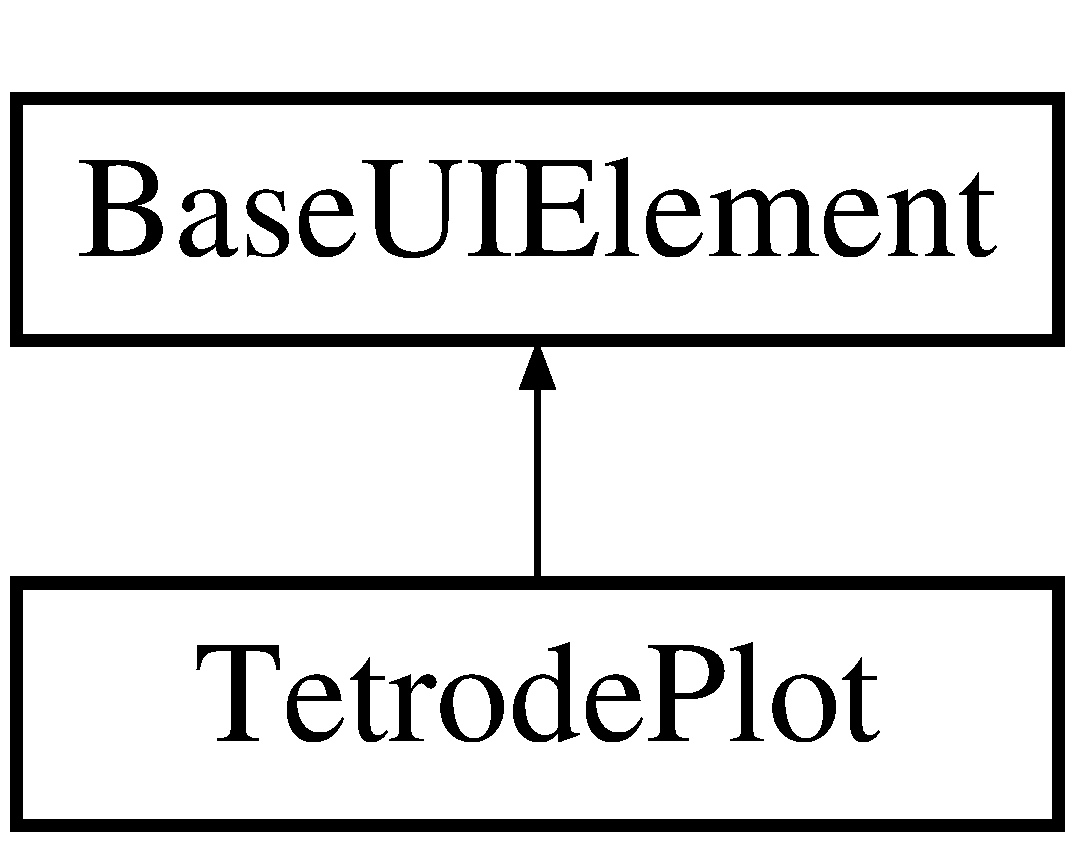
\includegraphics[height=2.000000cm]{classTetrodePlot}
\end{center}
\end{figure}
\subsection*{Public Member Functions}
\begin{DoxyCompactItemize}
\item 
\hypertarget{classTetrodePlot_a656ee6137f078f758e1be6dcfdddbc21}{{\bfseries Tetrode\-Plot} (int x, int y, int w, int h)}\label{classTetrodePlot_a656ee6137f078f758e1be6dcfdddbc21}

\item 
\hypertarget{classTetrodePlot_ae440c2b24680f270d8dd5458280c9d64}{void {\bfseries init\-Axes} ()}\label{classTetrodePlot_ae440c2b24680f270d8dd5458280c9d64}

\item 
\hypertarget{classTetrodePlot_a6d4494f6721849cad393a7be6ff6ef72}{void {\bfseries redraw} ()}\label{classTetrodePlot_a6d4494f6721849cad393a7be6ff6ef72}

\item 
\hypertarget{classTetrodePlot_a9791b6a0cc8f8378edbc37ff054feca2}{void {\bfseries set\-Enabled} (bool enabled)}\label{classTetrodePlot_a9791b6a0cc8f8378edbc37ff054feca2}

\item 
\hypertarget{classTetrodePlot_a9128abaa352225ddb4959408f8b30f2e}{bool {\bfseries get\-Enabled} ()}\label{classTetrodePlot_a9128abaa352225ddb4959408f8b30f2e}

\item 
\hypertarget{classTetrodePlot_ae3a380278f0197a92bb5a359a75553b8}{void {\bfseries set\-Position} (int, int, double, double)}\label{classTetrodePlot_ae3a380278f0197a92bb5a359a75553b8}

\item 
\hypertarget{classTetrodePlot_ac1c5202ac6a0ecfdcc846657c597b76d}{void {\bfseries get\-Preferred\-Dimensions} (double $\ast$, double $\ast$)}\label{classTetrodePlot_ac1c5202ac6a0ecfdcc846657c597b76d}

\item 
\hypertarget{classTetrodePlot_ae7a0c92060e12abe0c407324a4f572d8}{int {\bfseries get\-Number\-Of\-Axes} ()}\label{classTetrodePlot_ae7a0c92060e12abe0c407324a4f572d8}

\item 
\hypertarget{classTetrodePlot_abff5bd0246a2b648ebd6dfc1a0f93f4a}{void {\bfseries mouse\-Down} (int x, int y)}\label{classTetrodePlot_abff5bd0246a2b648ebd6dfc1a0f93f4a}

\item 
\hypertarget{classTetrodePlot_ae695cb5485e28e7eb925207fe0b89630}{void {\bfseries mouse\-Drag\-X} (int dx, bool shift, bool ctr)}\label{classTetrodePlot_ae695cb5485e28e7eb925207fe0b89630}

\item 
\hypertarget{classTetrodePlot_a3e14ad4c305364e1b935fe0574457735}{void {\bfseries mouse\-Drag\-Y} (int dy, bool shift, bool ctr)}\label{classTetrodePlot_a3e14ad4c305364e1b935fe0574457735}

\item 
\hypertarget{classTetrodePlot_aed9d207dbb3f6b08aeaf71232fbbbbd5}{bool {\bfseries process\-Key\-Event} (\hyperlink{structSimpleKeyEvent}{Simple\-Key\-Event} k)}\label{classTetrodePlot_aed9d207dbb3f6b08aeaf71232fbbbbd5}

\item 
\hypertarget{classTetrodePlot_abdd11b1351085b0398944fdfa514b747}{void {\bfseries process\-Spike\-Object} (\hyperlink{structSpikeObject}{Spike\-Object} s)}\label{classTetrodePlot_abdd11b1351085b0398944fdfa514b747}

\item 
\hypertarget{classTetrodePlot_a5135b3a4b280524ce48fa2167c266cd6}{void {\bfseries clear} ()}\label{classTetrodePlot_a5135b3a4b280524ce48fa2167c266cd6}

\item 
\hypertarget{classTetrodePlot_a86363d2346402271e993b31bcfde43fd}{void {\bfseries zoom} (int, bool)}\label{classTetrodePlot_a86363d2346402271e993b31bcfde43fd}

\item 
\hypertarget{classTetrodePlot_aed977b68cd1b2cfd2e155d58ec6f25da}{void {\bfseries pan} (int, bool)}\label{classTetrodePlot_aed977b68cd1b2cfd2e155d58ec6f25da}

\end{DoxyCompactItemize}
\subsection*{Private Member Functions}
\begin{DoxyCompactItemize}
\item 
\hypertarget{classTetrodePlot_a6ac2b954365575b90c3b4ea09bca05cb}{void {\bfseries init\-Limits} ()}\label{classTetrodePlot_a6ac2b954365575b90c3b4ea09bca05cb}

\item 
\hypertarget{classTetrodePlot_a6c55a9182b40a5f81e5c6ed13d3f9512}{void {\bfseries set\-Limits\-On\-Axes} ()}\label{classTetrodePlot_a6c55a9182b40a5f81e5c6ed13d3f9512}

\end{DoxyCompactItemize}
\subsection*{Private Attributes}
\begin{DoxyCompactItemize}
\item 
\hypertarget{classTetrodePlot_a108da4895456bcab9f9a09830fe4488b}{bool {\bfseries enabled}}\label{classTetrodePlot_a108da4895456bcab9f9a09830fe4488b}

\item 
\hypertarget{classTetrodePlot_a8b19fe1a2fe811922ae72726eb2920fa}{bool {\bfseries limits\-Changed}}\label{classTetrodePlot_a8b19fe1a2fe811922ae72726eb2920fa}

\item 
\hypertarget{classTetrodePlot_a563321643780b4c28b5625dbc68a0cbb}{double {\bfseries limits} \mbox{[}1\mbox{]}\mbox{[}2\mbox{]}}\label{classTetrodePlot_a563321643780b4c28b5625dbc68a0cbb}

\item 
\hypertarget{classTetrodePlot_adccda029fea54263cadda8346c3d1777}{\hyperlink{classWaveAxes}{Wave\-Axes} {\bfseries w\-Axes} \mbox{[}4\mbox{]}}\label{classTetrodePlot_adccda029fea54263cadda8346c3d1777}

\item 
\hypertarget{classTetrodePlot_a29821ae3a96010d4c4db91ab44b59424}{\hyperlink{classProjectionAxes}{Projection\-Axes} {\bfseries p\-Axes} \mbox{[}6\mbox{]}}\label{classTetrodePlot_a29821ae3a96010d4c4db91ab44b59424}

\end{DoxyCompactItemize}
\subsection*{Additional Inherited Members}


The documentation for this class was generated from the following file\-:\begin{DoxyCompactItemize}
\item 
Processors/\-Visualization/\-Spike\-Plotting/Tetrode\-Plot.\-h\end{DoxyCompactItemize}

\hypertarget{classThresholdSlider}{\section{Threshold\-Slider Class Reference}
\label{classThresholdSlider}\index{Threshold\-Slider@{Threshold\-Slider}}
}
\subsection*{Public Member Functions}
\begin{DoxyCompactItemize}
\item 
\hypertarget{classThresholdSlider_a5398c8e3554363cd303fa92882316ffd}{{\bfseries Threshold\-Slider} (Font f)}\label{classThresholdSlider_a5398c8e3554363cd303fa92882316ffd}

\item 
\hypertarget{classThresholdSlider_ac83ea11e9500f031115e483b24e1a5c7}{void {\bfseries set\-Active} (bool)}\label{classThresholdSlider_ac83ea11e9500f031115e483b24e1a5c7}

\item 
\hypertarget{classThresholdSlider_a9f1539033db04ee192efd8797c6de47e}{void {\bfseries set\-Values} (Array$<$ double $>$)}\label{classThresholdSlider_a9f1539033db04ee192efd8797c6de47e}

\end{DoxyCompactItemize}
\subsection*{Private Member Functions}
\begin{DoxyCompactItemize}
\item 
\hypertarget{classThresholdSlider_a61dc99677aec47179be42eb57f6f27d8}{void {\bfseries paint} (Graphics \&g)}\label{classThresholdSlider_a61dc99677aec47179be42eb57f6f27d8}

\item 
\hypertarget{classThresholdSlider_a7c3fe6e93477cb6280c44dd8dde8ccc8}{Path {\bfseries make\-Rotary\-Path} (double, double, double)}\label{classThresholdSlider_a7c3fe6e93477cb6280c44dd8dde8ccc8}

\end{DoxyCompactItemize}
\subsection*{Private Attributes}
\begin{DoxyCompactItemize}
\item 
\hypertarget{classThresholdSlider_a8a9253483d81108291ae60a4ac33e9e7}{Font {\bfseries font}}\label{classThresholdSlider_a8a9253483d81108291ae60a4ac33e9e7}

\item 
\hypertarget{classThresholdSlider_a79e4ddcfe860a4ed441f834aa28237ef}{bool {\bfseries is\-Active}}\label{classThresholdSlider_a79e4ddcfe860a4ed441f834aa28237ef}

\item 
\hypertarget{classThresholdSlider_a1e0ae8d93bca3f3321d2f051e8ec3fc6}{Array$<$ double $>$ {\bfseries value\-Array}}\label{classThresholdSlider_a1e0ae8d93bca3f3321d2f051e8ec3fc6}

\end{DoxyCompactItemize}


The documentation for this class was generated from the following file\-:\begin{DoxyCompactItemize}
\item 
Processors/\-Editors/Spike\-Detector\-Editor.\-h\end{DoxyCompactItemize}

\hypertarget{classTriangleButton}{\section{Triangle\-Button Class Reference}
\label{classTriangleButton}\index{Triangle\-Button@{Triangle\-Button}}
}
\subsection*{Public Member Functions}
\begin{DoxyCompactItemize}
\item 
\hypertarget{classTriangleButton_a91e0ca3f1db5448686b2ed45f5cdf21b}{{\bfseries Triangle\-Button} (int direction\-\_\-)}\label{classTriangleButton_a91e0ca3f1db5448686b2ed45f5cdf21b}

\end{DoxyCompactItemize}
\subsection*{Private Member Functions}
\begin{DoxyCompactItemize}
\item 
\hypertarget{classTriangleButton_a396bef56f305e84b677537c4343ed96b}{void {\bfseries paint\-Button} (Graphics \&g, bool is\-Mouse\-Over, bool is\-Button\-Down)}\label{classTriangleButton_a396bef56f305e84b677537c4343ed96b}

\end{DoxyCompactItemize}
\subsection*{Private Attributes}
\begin{DoxyCompactItemize}
\item 
\hypertarget{classTriangleButton_ad9a2fa34e8e4c171bfb0f03d67d7aae6}{int {\bfseries direction}}\label{classTriangleButton_ad9a2fa34e8e4c171bfb0f03d67d7aae6}

\end{DoxyCompactItemize}


The documentation for this class was generated from the following file\-:\begin{DoxyCompactItemize}
\item 
Processors/\-Editors/Generic\-Editor.\-h\end{DoxyCompactItemize}

\hypertarget{classUIComponent}{\section{U\-I\-Component Class Reference}
\label{classUIComponent}\index{U\-I\-Component@{U\-I\-Component}}
}
\subsection*{Public Member Functions}
\begin{DoxyCompactItemize}
\item 
\hypertarget{classUIComponent_a4fa1a33a7e8d5edc2b60b14ac49639aa}{{\bfseries U\-I\-Component} (\hyperlink{classMainWindow}{Main\-Window} $\ast$main\-Window\-\_\-, \hyperlink{classProcessorGraph}{Processor\-Graph} $\ast$pgraph, \hyperlink{classAudioComponent}{Audio\-Component} $\ast$audio)}\label{classUIComponent_a4fa1a33a7e8d5edc2b60b14ac49639aa}

\item 
\hypertarget{classUIComponent_a764410a9d82b5d45a32e0de989277ce4}{\hyperlink{classEditorViewport}{Editor\-Viewport} $\ast$ {\bfseries get\-Editor\-Viewport} ()}\label{classUIComponent_a764410a9d82b5d45a32e0de989277ce4}

\item 
\hypertarget{classUIComponent_ad12419d300debb7c4386bd4d06118bbc}{\hyperlink{classProcessorList}{Processor\-List} $\ast$ {\bfseries get\-Processor\-List} ()}\label{classUIComponent_ad12419d300debb7c4386bd4d06118bbc}

\item 
\hypertarget{classUIComponent_a811c6b70bca15049bde52d92ddc8b3ba}{\hyperlink{classDataViewport}{Data\-Viewport} $\ast$ {\bfseries get\-Data\-Viewport} ()}\label{classUIComponent_a811c6b70bca15049bde52d92ddc8b3ba}

\item 
\hypertarget{classUIComponent_acd2f9e680aec22ec9ead4e311f744d27}{\hyperlink{classProcessorGraph}{Processor\-Graph} $\ast$ {\bfseries get\-Processor\-Graph} ()}\label{classUIComponent_acd2f9e680aec22ec9ead4e311f744d27}

\item 
\hypertarget{classUIComponent_a8030cf8a31ec7abe27c01dc1ca5049b8}{\hyperlink{classControlPanel}{Control\-Panel} $\ast$ {\bfseries get\-Control\-Panel} ()}\label{classUIComponent_a8030cf8a31ec7abe27c01dc1ca5049b8}

\item 
\hypertarget{classUIComponent_a3990b3973b9f9e6105f2a05e44b02006}{\hyperlink{classMessageCenter}{Message\-Center} $\ast$ {\bfseries get\-Message\-Center} ()}\label{classUIComponent_a3990b3973b9f9e6105f2a05e44b02006}

\item 
\hypertarget{classUIComponent_a398c3ed66856fece160315e40e48f47c}{\hyperlink{classUIComponent}{U\-I\-Component} $\ast$ {\bfseries get\-U\-I\-Component} ()}\label{classUIComponent_a398c3ed66856fece160315e40e48f47c}

\item 
\hypertarget{classUIComponent_aaad1ad4aba78ee21389c685d1804bb06}{\hyperlink{classAudioComponent}{Audio\-Component} $\ast$ {\bfseries get\-Audio\-Component} ()}\label{classUIComponent_aaad1ad4aba78ee21389c685d1804bb06}

\item 
\hypertarget{classUIComponent_a38a23101bdc53813595dc71f54049e2b}{void {\bfseries disable\-Callbacks} ()}\label{classUIComponent_a38a23101bdc53813595dc71f54049e2b}

\item 
\hypertarget{classUIComponent_ad14aea4dcdb95649748ba5f9575858e9}{void {\bfseries disable\-Data\-Viewport} ()}\label{classUIComponent_ad14aea4dcdb95649748ba5f9575858e9}

\item 
\hypertarget{classUIComponent_a59aefb9581d3e44318a2d1f2a446a31f}{void {\bfseries child\-Component\-Changed} ()}\label{classUIComponent_a59aefb9581d3e44318a2d1f2a446a31f}

\item 
\hypertarget{classUIComponent_a00b52a772ffea55b942c0def87be1ea9}{const String\-Array {\bfseries get\-Menu\-Bar\-Names} ()}\label{classUIComponent_a00b52a772ffea55b942c0def87be1ea9}

\item 
\hypertarget{classUIComponent_ad401a7a0c4096f012e19f8fc4cc5021b}{const Popup\-Menu {\bfseries get\-Menu\-For\-Index} (int top\-Level\-Menu\-Index, const String \&menu\-Name)}\label{classUIComponent_ad401a7a0c4096f012e19f8fc4cc5021b}

\item 
\hypertarget{classUIComponent_a011b702a81af51214ec797416cfe5b6c}{void {\bfseries menu\-Item\-Selected} (int menu\-Item\-I\-D, int top\-Level\-Menu\-Index)}\label{classUIComponent_a011b702a81af51214ec797416cfe5b6c}

\item 
\hypertarget{classUIComponent_ad0b6f699bb84ccbb2c341940845e49b9}{Application\-Command\-Target $\ast$ {\bfseries get\-Next\-Command\-Target} ()}\label{classUIComponent_ad0b6f699bb84ccbb2c341940845e49b9}

\item 
\hypertarget{classUIComponent_a292cf43e909207876e2dac2d70f54635}{void {\bfseries get\-All\-Commands} (Array$<$ Command\-I\-D $>$ \&commands)}\label{classUIComponent_a292cf43e909207876e2dac2d70f54635}

\item 
\hypertarget{classUIComponent_ab375e1b7c1b1ab4640ed35f4adc9504a}{void {\bfseries get\-Command\-Info} (Command\-I\-D command\-I\-D, Application\-Command\-Info \&result)}\label{classUIComponent_ab375e1b7c1b1ab4640ed35f4adc9504a}

\item 
\hypertarget{classUIComponent_a6d87ca3ae47d93c7288689fddf5d6c51}{bool {\bfseries perform} (const Invocation\-Info \&info)}\label{classUIComponent_a6d87ca3ae47d93c7288689fddf5d6c51}

\end{DoxyCompactItemize}
\subsection*{Private Types}
\begin{DoxyCompactItemize}
\item 
enum {\bfseries Command\-I\-Ds} \{ \\*
{\bfseries open\-Configuration} =  0x2001, 
{\bfseries save\-Configuration} =  0x2002, 
{\bfseries undo} =  0x2003, 
{\bfseries redo} =  0x2004, 
\\*
{\bfseries copy\-Signal\-Chain} =  0x2005, 
{\bfseries paste\-Signal\-Chain} =  0x2006, 
{\bfseries clear\-Signal\-Chain} =  0x2007, 
{\bfseries toggle\-Processor\-List} =  0x2008, 
\\*
{\bfseries toggle\-Signal\-Chain} =  0x2009, 
{\bfseries toggle\-File\-Info} =  0x2010, 
{\bfseries show\-Help} =  0x2011
 \}
\end{DoxyCompactItemize}
\subsection*{Private Member Functions}
\begin{DoxyCompactItemize}
\item 
\hypertarget{classUIComponent_a3cf1c579fc0c309d50ffbb83c7534cc7}{void {\bfseries resized} ()}\label{classUIComponent_a3cf1c579fc0c309d50ffbb83c7534cc7}

\item 
\hypertarget{classUIComponent_a4e5869c0da489213df444e63e56580f9}{{\bfseries J\-U\-C\-E\-\_\-\-D\-E\-C\-L\-A\-R\-E\-\_\-\-N\-O\-N\-\_\-\-C\-O\-P\-Y\-A\-B\-L\-E\-\_\-\-W\-I\-T\-H\-\_\-\-L\-E\-A\-K\-\_\-\-D\-E\-T\-E\-C\-T\-O\-R} (\hyperlink{classUIComponent}{U\-I\-Component})}\label{classUIComponent_a4e5869c0da489213df444e63e56580f9}

\end{DoxyCompactItemize}
\subsection*{Private Attributes}
\begin{DoxyCompactItemize}
\item 
\hypertarget{classUIComponent_a9d68e7a3a6a74613cba2152c14be3edf}{\hyperlink{classDataViewport}{Data\-Viewport} $\ast$ {\bfseries data\-Viewport}}\label{classUIComponent_a9d68e7a3a6a74613cba2152c14be3edf}

\item 
\hypertarget{classUIComponent_a04b249e3f62b57843fd02003606ff3d5}{\hyperlink{classEditorViewport}{Editor\-Viewport} $\ast$ {\bfseries editor\-Viewport}}\label{classUIComponent_a04b249e3f62b57843fd02003606ff3d5}

\item 
\hypertarget{classUIComponent_a75d4c61867b0f22ed838571a5747ef28}{\hyperlink{classEditorViewportButton}{Editor\-Viewport\-Button} $\ast$ {\bfseries editor\-Viewport\-Button}}\label{classUIComponent_a75d4c61867b0f22ed838571a5747ef28}

\item 
\hypertarget{classUIComponent_aad88597bcb3ed932d77d630e8788660c}{\hyperlink{classProcessorList}{Processor\-List} $\ast$ {\bfseries processor\-List}}\label{classUIComponent_aad88597bcb3ed932d77d630e8788660c}

\item 
\hypertarget{classUIComponent_a33bd55250d5ac56d8fb14d0674d183d9}{\hyperlink{classControlPanel}{Control\-Panel} $\ast$ {\bfseries control\-Panel}}\label{classUIComponent_a33bd55250d5ac56d8fb14d0674d183d9}

\item 
\hypertarget{classUIComponent_ac1cf64f19c2d9498bf51ca48862d1d29}{\hyperlink{classMessageCenter}{Message\-Center} $\ast$ {\bfseries message\-Center}}\label{classUIComponent_ac1cf64f19c2d9498bf51ca48862d1d29}

\item 
\hypertarget{classUIComponent_aaf91b15a8e81dbb6dc2d8b25a5937702}{\hyperlink{classInfoLabel}{Info\-Label} $\ast$ {\bfseries info\-Label}}\label{classUIComponent_aaf91b15a8e81dbb6dc2d8b25a5937702}

\item 
\hypertarget{classUIComponent_a664b9f862a4e9922729184fc76b5fd40}{\hyperlink{classMainWindow}{Main\-Window} $\ast$ {\bfseries main\-Window}}\label{classUIComponent_a664b9f862a4e9922729184fc76b5fd40}

\item 
\hypertarget{classUIComponent_aada41b9c0296382931f51a455b7748fb}{Tooltip\-Window {\bfseries tooltip\-Window}}\label{classUIComponent_aada41b9c0296382931f51a455b7748fb}

\item 
\hypertarget{classUIComponent_a677e808911329a5e9c302ce66686950e}{\hyperlink{classProcessorGraph}{Processor\-Graph} $\ast$ {\bfseries processor\-Graph}}\label{classUIComponent_a677e808911329a5e9c302ce66686950e}

\item 
\hypertarget{classUIComponent_a9545ca4f43092f5b20523da9f12c1395}{\hyperlink{classAudioComponent}{Audio\-Component} $\ast$ {\bfseries audio}}\label{classUIComponent_a9545ca4f43092f5b20523da9f12c1395}

\end{DoxyCompactItemize}


The documentation for this class was generated from the following file\-:\begin{DoxyCompactItemize}
\item 
U\-I/U\-I\-Component.\-h\end{DoxyCompactItemize}

\hypertarget{classUtilityButton}{\section{Utility\-Button Class Reference}
\label{classUtilityButton}\index{Utility\-Button@{Utility\-Button}}
}
\subsection*{Public Member Functions}
\begin{DoxyCompactItemize}
\item 
\hypertarget{classUtilityButton_a5eefdacd94ea6636c1671bd30268ae76}{{\bfseries Utility\-Button} (const String \&label\-\_\-, Font font\-\_\-)}\label{classUtilityButton_a5eefdacd94ea6636c1671bd30268ae76}

\item 
\hypertarget{classUtilityButton_adae51ec7dbb328f92aeee30d0b96ea80}{void {\bfseries set\-Corners} (bool U\-L, bool U\-R, bool L\-L, bool L\-R)}\label{classUtilityButton_adae51ec7dbb328f92aeee30d0b96ea80}

\item 
\hypertarget{classUtilityButton_aa703482b887e1f8d4b123cf11549619a}{void {\bfseries set\-Radius} (float r)}\label{classUtilityButton_aa703482b887e1f8d4b123cf11549619a}

\item 
\hypertarget{classUtilityButton_a81ac09396e3475f7d3ec20299b1ba445}{void {\bfseries set\-Enabled\-State} (bool)}\label{classUtilityButton_a81ac09396e3475f7d3ec20299b1ba445}

\item 
\hypertarget{classUtilityButton_a247a7d048da7deb4f4b8537f1cce05e4}{bool {\bfseries get\-Enabled\-State} ()}\label{classUtilityButton_a247a7d048da7deb4f4b8537f1cce05e4}

\end{DoxyCompactItemize}
\subsection*{Private Member Functions}
\begin{DoxyCompactItemize}
\item 
\hypertarget{classUtilityButton_aaa24c18aee5f1df3ee10277a8f558f3a}{void {\bfseries paint\-Button} (Graphics \&g, bool is\-Mouse\-Over, bool is\-Button\-Down)}\label{classUtilityButton_aaa24c18aee5f1df3ee10277a8f558f3a}

\item 
\hypertarget{classUtilityButton_ac08e08174673146fddc257f3bc5972d1}{void {\bfseries resized} ()}\label{classUtilityButton_ac08e08174673146fddc257f3bc5972d1}

\end{DoxyCompactItemize}
\subsection*{Private Attributes}
\begin{DoxyCompactItemize}
\item 
\hypertarget{classUtilityButton_aa546e57b46b8421960a2f44356519374}{const String {\bfseries label}}\label{classUtilityButton_aa546e57b46b8421960a2f44356519374}

\item 
\hypertarget{classUtilityButton_a167cd427e65ee235d7cd7cbf1c5bd0b1}{Font {\bfseries font}}\label{classUtilityButton_a167cd427e65ee235d7cd7cbf1c5bd0b1}

\item 
\hypertarget{classUtilityButton_a5764d2ecaf8d351ddfec645cc5c8c9b8}{bool {\bfseries round\-U\-L}}\label{classUtilityButton_a5764d2ecaf8d351ddfec645cc5c8c9b8}

\item 
\hypertarget{classUtilityButton_a28ac7cdc8989d02ed9de37fee2a69d60}{bool {\bfseries round\-U\-R}}\label{classUtilityButton_a28ac7cdc8989d02ed9de37fee2a69d60}

\item 
\hypertarget{classUtilityButton_abe36ec1a745ae8038577a93b83cc64a8}{bool {\bfseries round\-L\-L}}\label{classUtilityButton_abe36ec1a745ae8038577a93b83cc64a8}

\item 
\hypertarget{classUtilityButton_ae164d537e1a9de5b4876aea19091468f}{bool {\bfseries round\-L\-R}}\label{classUtilityButton_ae164d537e1a9de5b4876aea19091468f}

\item 
\hypertarget{classUtilityButton_ab077438a18aee979e440f8e240cf7ec7}{float {\bfseries radius}}\label{classUtilityButton_ab077438a18aee979e440f8e240cf7ec7}

\item 
\hypertarget{classUtilityButton_a69b52bad0ed0e10436b850db09822d5f}{Colour\-Gradient {\bfseries selected\-Grad}}\label{classUtilityButton_a69b52bad0ed0e10436b850db09822d5f}

\item 
\hypertarget{classUtilityButton_a1a8c608e3e9accf5ffbc66ad182d61e3}{Colour\-Gradient {\bfseries selected\-Over\-Grad}}\label{classUtilityButton_a1a8c608e3e9accf5ffbc66ad182d61e3}

\item 
\hypertarget{classUtilityButton_a18ca4f6648554c0f744f09ee78365843}{Colour\-Gradient {\bfseries neutral\-Grad}}\label{classUtilityButton_a18ca4f6648554c0f744f09ee78365843}

\item 
\hypertarget{classUtilityButton_aa808a3cb8673c8148fee1450ce7c4648}{Colour\-Gradient {\bfseries neutral\-Over\-Grad}}\label{classUtilityButton_aa808a3cb8673c8148fee1450ce7c4648}

\item 
\hypertarget{classUtilityButton_ae32c460e56bbeaaa7ab2bcd9081bb35c}{Colour {\bfseries font\-Color}}\label{classUtilityButton_ae32c460e56bbeaaa7ab2bcd9081bb35c}

\item 
\hypertarget{classUtilityButton_a70fe4c7e3ad6f5267bbcc304f324747c}{Path {\bfseries outline\-Path}}\label{classUtilityButton_a70fe4c7e3ad6f5267bbcc304f324747c}

\item 
\hypertarget{classUtilityButton_ae37208d29f863b9405b5990016c13ce3}{bool {\bfseries is\-Enabled}}\label{classUtilityButton_ae37208d29f863b9405b5990016c13ce3}

\end{DoxyCompactItemize}


The documentation for this class was generated from the following file\-:\begin{DoxyCompactItemize}
\item 
Processors/\-Editors/Generic\-Editor.\-h\end{DoxyCompactItemize}

\hypertarget{classVisualizer}{\section{Visualizer Class Reference}
\label{classVisualizer}\index{Visualizer@{Visualizer}}
}
Inheritance diagram for Visualizer\-:\begin{figure}[H]
\begin{center}
\leavevmode
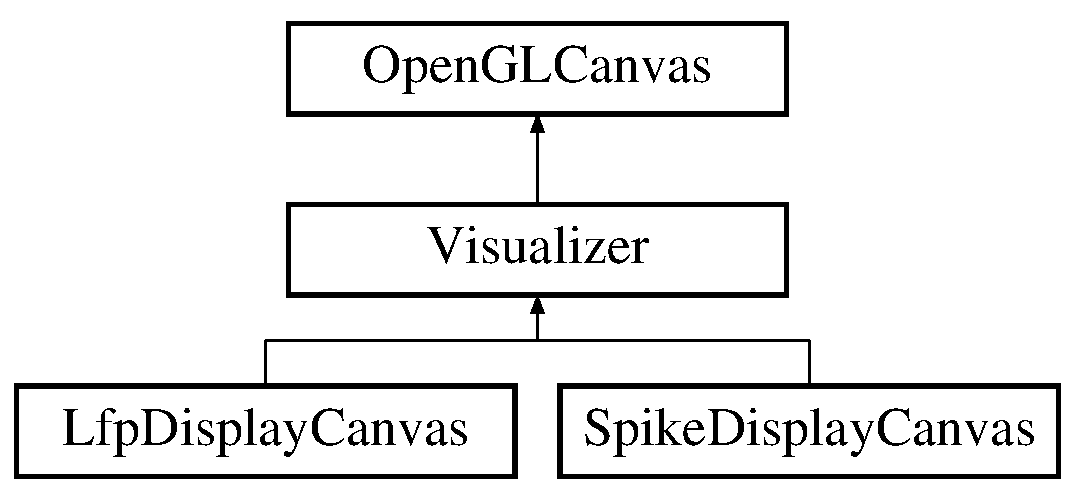
\includegraphics[height=3.000000cm]{classVisualizer}
\end{center}
\end{figure}
\subsection*{Public Member Functions}
\begin{DoxyCompactItemize}
\item 
\hypertarget{classVisualizer_ad68a445fc8dcd77c1f49c354ba888807}{virtual void {\bfseries new\-Open\-G\-L\-Context\-Created} ()=0}\label{classVisualizer_ad68a445fc8dcd77c1f49c354ba888807}

\item 
\hypertarget{classVisualizer_a50903eb0365edf476d1323d41719f8ff}{virtual void {\bfseries render\-Open\-G\-L} ()=0}\label{classVisualizer_a50903eb0365edf476d1323d41719f8ff}

\item 
\hypertarget{classVisualizer_a2a5ff831cf144f1fd887395f055d9ed4}{virtual void {\bfseries refresh\-State} ()=0}\label{classVisualizer_a2a5ff831cf144f1fd887395f055d9ed4}

\item 
\hypertarget{classVisualizer_a0fe43ca2f65258eeb5612a52495d4ce5}{virtual void {\bfseries update} ()=0}\label{classVisualizer_a0fe43ca2f65258eeb5612a52495d4ce5}

\item 
\hypertarget{classVisualizer_ae77321ed5287628e8d6c11728f480138}{virtual int {\bfseries get\-Total\-Height} ()=0}\label{classVisualizer_ae77321ed5287628e8d6c11728f480138}

\item 
\hypertarget{classVisualizer_a0be9e571d391521a48f55a509487d0e7}{virtual void {\bfseries begin\-Animation} ()=0}\label{classVisualizer_a0be9e571d391521a48f55a509487d0e7}

\item 
\hypertarget{classVisualizer_a990653e6c62bd9e7fbc183fd14820a4f}{virtual void {\bfseries end\-Animation} ()=0}\label{classVisualizer_a990653e6c62bd9e7fbc183fd14820a4f}

\item 
\hypertarget{classVisualizer_a6ff2b57ce80c2baec048c467792cc301}{virtual void {\bfseries set\-Parameter} (int, float)=0}\label{classVisualizer_a6ff2b57ce80c2baec048c467792cc301}

\item 
\hypertarget{classVisualizer_a44b37adda5e799112ca835442a977d06}{virtual void {\bfseries set\-Parameter} (int, int, int, float)=0}\label{classVisualizer_a44b37adda5e799112ca835442a977d06}

\end{DoxyCompactItemize}
\subsection*{Additional Inherited Members}


The documentation for this class was generated from the following file\-:\begin{DoxyCompactItemize}
\item 
Processors/\-Visualization/Visualizer.\-h\end{DoxyCompactItemize}

\hypertarget{classVisualizerEditor}{\section{Visualizer\-Editor Class Reference}
\label{classVisualizerEditor}\index{Visualizer\-Editor@{Visualizer\-Editor}}
}
Inheritance diagram for Visualizer\-Editor\-:\begin{figure}[H]
\begin{center}
\leavevmode
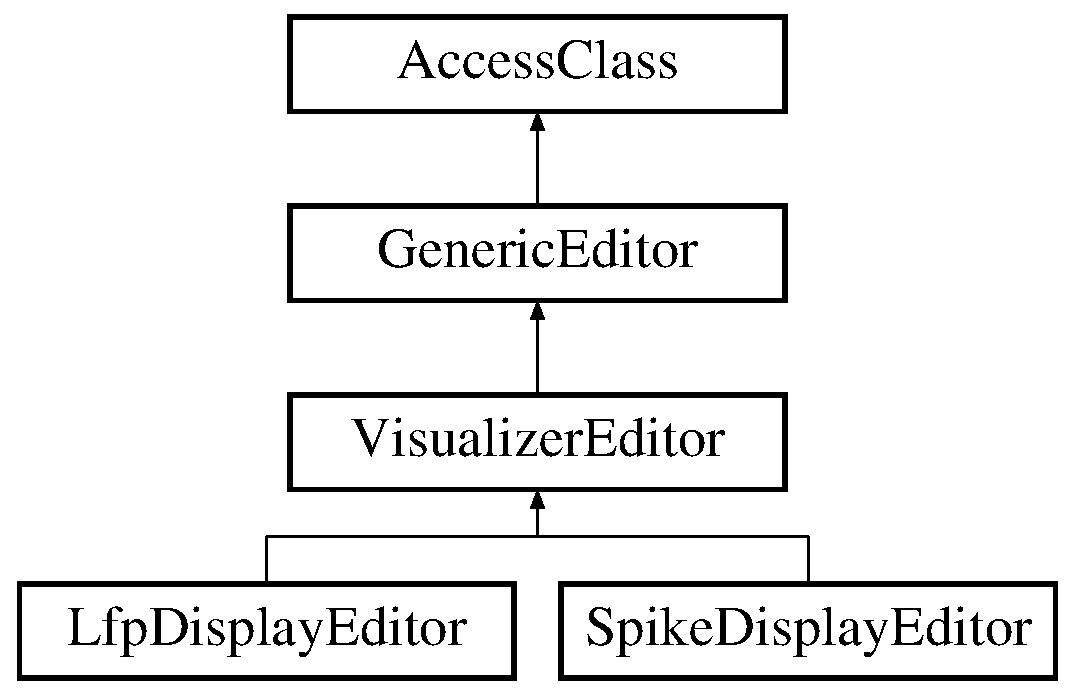
\includegraphics[height=4.000000cm]{classVisualizerEditor}
\end{center}
\end{figure}
\subsection*{Public Member Functions}
\begin{DoxyCompactItemize}
\item 
\hypertarget{classVisualizerEditor_a42310e08d09f3f6d933959b1af373eb8}{{\bfseries Visualizer\-Editor} (\hyperlink{classGenericProcessor}{Generic\-Processor} $\ast$, int)}\label{classVisualizerEditor_a42310e08d09f3f6d933959b1af373eb8}

\item 
\hypertarget{classVisualizerEditor_a0b39da0ca87e1ae2642787bc53d2772c}{{\bfseries Visualizer\-Editor} (\hyperlink{classGenericProcessor}{Generic\-Processor} $\ast$)}\label{classVisualizerEditor_a0b39da0ca87e1ae2642787bc53d2772c}

\item 
\hypertarget{classVisualizerEditor_a5f0dc2c7132660a5ce1fd9d5cbc9c6ff}{void {\bfseries button\-Event} (Button $\ast$button)}\label{classVisualizerEditor_a5f0dc2c7132660a5ce1fd9d5cbc9c6ff}

\item 
\hypertarget{classVisualizerEditor_a28603b8f37f5d74a064cee42981be368}{virtual void {\bfseries button\-Callback} (Button $\ast$button)}\label{classVisualizerEditor_a28603b8f37f5d74a064cee42981be368}

\item 
\hypertarget{classVisualizerEditor_ad9e8d76310366869e3f2f51ac4a2dc65}{virtual \hyperlink{classVisualizer}{Visualizer} $\ast$ {\bfseries create\-New\-Canvas} ()=0}\label{classVisualizerEditor_ad9e8d76310366869e3f2f51ac4a2dc65}

\item 
\hypertarget{classVisualizerEditor_a784c317c2b9bb06e25e287c4ecf0670e}{virtual void {\bfseries enable} ()}\label{classVisualizerEditor_a784c317c2b9bb06e25e287c4ecf0670e}

\item 
\hypertarget{classVisualizerEditor_a9277b0aa356ea41040b9c9960abda21b}{virtual void {\bfseries disable} ()}\label{classVisualizerEditor_a9277b0aa356ea41040b9c9960abda21b}

\item 
\hypertarget{classVisualizerEditor_a852c519636c0428a2d2b2b7219108f67}{void {\bfseries editor\-Was\-Clicked} ()}\label{classVisualizerEditor_a852c519636c0428a2d2b2b7219108f67}

\item 
\hypertarget{classVisualizerEditor_a11c5e6386531cff49e6babfeb18a8885}{void {\bfseries update\-Visualizer} ()}\label{classVisualizerEditor_a11c5e6386531cff49e6babfeb18a8885}

\end{DoxyCompactItemize}
\subsection*{Public Attributes}
\begin{DoxyCompactItemize}
\item 
\hypertarget{classVisualizerEditor_ab8caef8de0f8eeedb81a936d81b354bc}{Scoped\-Pointer$<$ \hyperlink{classDataWindow}{Data\-Window} $>$ {\bfseries data\-Window}}\label{classVisualizerEditor_ab8caef8de0f8eeedb81a936d81b354bc}

\item 
\hypertarget{classVisualizerEditor_a31c5fc40fd3bb3f3777a600c75c57171}{Scoped\-Pointer$<$ \hyperlink{classVisualizer}{Visualizer} $>$ {\bfseries canvas}}\label{classVisualizerEditor_a31c5fc40fd3bb3f3777a600c75c57171}

\item 
\hypertarget{classVisualizerEditor_a3a412027e66432c1d399e00a089f414e}{String {\bfseries tab\-Text}}\label{classVisualizerEditor_a3a412027e66432c1d399e00a089f414e}

\end{DoxyCompactItemize}
\subsection*{Private Member Functions}
\begin{DoxyCompactItemize}
\item 
\hypertarget{classVisualizerEditor_a4bd8aa75dfee06f821fbea618ea6fced}{void {\bfseries initialize\-Selectors} ()}\label{classVisualizerEditor_a4bd8aa75dfee06f821fbea618ea6fced}

\item 
\hypertarget{classVisualizerEditor_a1b471d9680da48e36672ba9865f2f873}{{\bfseries J\-U\-C\-E\-\_\-\-D\-E\-C\-L\-A\-R\-E\-\_\-\-N\-O\-N\-\_\-\-C\-O\-P\-Y\-A\-B\-L\-E\-\_\-\-W\-I\-T\-H\-\_\-\-L\-E\-A\-K\-\_\-\-D\-E\-T\-E\-C\-T\-O\-R} (\hyperlink{classVisualizerEditor}{Visualizer\-Editor})}\label{classVisualizerEditor_a1b471d9680da48e36672ba9865f2f873}

\end{DoxyCompactItemize}
\subsection*{Private Attributes}
\begin{DoxyCompactItemize}
\item 
\hypertarget{classVisualizerEditor_af4ba7076b26c11ae8e2dc6fb33d3c8f4}{bool {\bfseries is\-Playing}}\label{classVisualizerEditor_af4ba7076b26c11ae8e2dc6fb33d3c8f4}

\item 
\hypertarget{classVisualizerEditor_a064cde76d690f3fefb6d7d529542387d}{\hyperlink{classSelectorButton}{Selector\-Button} $\ast$ {\bfseries window\-Selector}}\label{classVisualizerEditor_a064cde76d690f3fefb6d7d529542387d}

\item 
\hypertarget{classVisualizerEditor_a2f6bf303ca3d0b250bc6b9df2505360a}{\hyperlink{classSelectorButton}{Selector\-Button} $\ast$ {\bfseries tab\-Selector}}\label{classVisualizerEditor_a2f6bf303ca3d0b250bc6b9df2505360a}

\item 
\hypertarget{classVisualizerEditor_a9cd7fd0eaaddb352342f5d76de5cdb57}{int {\bfseries tab\-Index}}\label{classVisualizerEditor_a9cd7fd0eaaddb352342f5d76de5cdb57}

\end{DoxyCompactItemize}
\subsection*{Additional Inherited Members}


The documentation for this class was generated from the following file\-:\begin{DoxyCompactItemize}
\item 
Processors/\-Editors/Visualizer\-Editor.\-h\end{DoxyCompactItemize}

\hypertarget{classWaveAxes}{\section{Wave\-Axes Class Reference}
\label{classWaveAxes}\index{Wave\-Axes@{Wave\-Axes}}
}
Inheritance diagram for Wave\-Axes\-:\begin{figure}[H]
\begin{center}
\leavevmode
\includegraphics[height=3.000000cm]{classWaveAxes}
\end{center}
\end{figure}
\subsection*{Public Member Functions}
\begin{DoxyCompactItemize}
\item 
\hypertarget{classWaveAxes_a3e1b38a080b666c68e6b9f038ac5ed3d}{{\bfseries Wave\-Axes} (int x, int y, double w, double h, int t)}\label{classWaveAxes_a3e1b38a080b666c68e6b9f038ac5ed3d}

\item 
\hypertarget{classWaveAxes_a4850fe1b808de00c9a8b44e859cea21e}{void {\bfseries update\-Spike\-Data} (\hyperlink{structSpikeObject}{Spike\-Object} s)}\label{classWaveAxes_a4850fe1b808de00c9a8b44e859cea21e}

\item 
\hypertarget{classWaveAxes_a31f253cb5b82309e8824ec9892eda266}{void {\bfseries set\-Waveform\-Color} (G\-Lfloat r, G\-Lfloat g, G\-Lfloat b)}\label{classWaveAxes_a31f253cb5b82309e8824ec9892eda266}

\item 
\hypertarget{classWaveAxes_ac7eb4c088dfe493ff3304681321c1d9e}{void {\bfseries set\-Threshold\-Color} (G\-Lfloat r, G\-Lfloat g, G\-Lfloat b)}\label{classWaveAxes_ac7eb4c088dfe493ff3304681321c1d9e}

\item 
\hypertarget{classWaveAxes_a2434fce7713b5d48d8f8b1175fd1d4d4}{void {\bfseries set\-Grid\-Color} (G\-Lfloat, G\-Lfloat, G\-Lfloat)}\label{classWaveAxes_a2434fce7713b5d48d8f8b1175fd1d4d4}

\item 
\hypertarget{classWaveAxes_a45afcfea4c34075e6d73786642846bd5}{void {\bfseries redraw} ()}\label{classWaveAxes_a45afcfea4c34075e6d73786642846bd5}

\end{DoxyCompactItemize}
\subsection*{Public Attributes}
\begin{DoxyCompactItemize}
\item 
\hypertarget{classWaveAxes_a76257ba1d18136073d166d644e705531}{bool {\bfseries draw\-Waveform\-Line}}\label{classWaveAxes_a76257ba1d18136073d166d644e705531}

\item 
\hypertarget{classWaveAxes_a7a8fdc89f6d4f0dedc6711ad3500c358}{bool {\bfseries draw\-Waveform\-Points}}\label{classWaveAxes_a7a8fdc89f6d4f0dedc6711ad3500c358}

\item 
\hypertarget{classWaveAxes_a48c33abae62a2c2449c5ed19436f44ca}{bool {\bfseries overlay}}\label{classWaveAxes_a48c33abae62a2c2449c5ed19436f44ca}

\item 
\hypertarget{classWaveAxes_abec2c03401e4f4282238a164153ec17d}{bool {\bfseries draw\-Grid}}\label{classWaveAxes_abec2c03401e4f4282238a164153ec17d}

\item 
\hypertarget{classWaveAxes_ad3f862d07a773b1259cf7cc027aab21b}{bool {\bfseries convert\-Label\-Units}}\label{classWaveAxes_ad3f862d07a773b1259cf7cc027aab21b}

\end{DoxyCompactItemize}
\subsection*{Protected Member Functions}
\begin{DoxyCompactItemize}
\item 
\hypertarget{classWaveAxes_a9b247805f9b3962b1a31a935a73de6a6}{void {\bfseries plot} ()}\label{classWaveAxes_a9b247805f9b3962b1a31a935a73de6a6}

\end{DoxyCompactItemize}
\subsection*{Private Member Functions}
\begin{DoxyCompactItemize}
\item 
\hypertarget{classWaveAxes_ac2e6744baeb75b0133e09c795cbca415}{void {\bfseries draw\-Waveform\-Grid} (int thold, int gain)}\label{classWaveAxes_ac2e6744baeb75b0133e09c795cbca415}

\end{DoxyCompactItemize}
\subsection*{Private Attributes}
\begin{DoxyCompactItemize}
\item 
\hypertarget{classWaveAxes_ad58b6a65b3bf0b5315d036356eefe292}{G\-Lfloat {\bfseries wave\-Color} \mbox{[}3\mbox{]}}\label{classWaveAxes_ad58b6a65b3bf0b5315d036356eefe292}

\item 
\hypertarget{classWaveAxes_acd4a9eb44178c4512d5af14fb3c0580f}{G\-Lfloat {\bfseries threshold\-Color} \mbox{[}3\mbox{]}}\label{classWaveAxes_acd4a9eb44178c4512d5af14fb3c0580f}

\item 
\hypertarget{classWaveAxes_a0de2e59894e1ac946c0b523d689fb22e}{G\-Lfloat {\bfseries grid\-Color} \mbox{[}3\mbox{]}}\label{classWaveAxes_a0de2e59894e1ac946c0b523d689fb22e}

\end{DoxyCompactItemize}
\subsection*{Additional Inherited Members}


The documentation for this class was generated from the following file\-:\begin{DoxyCompactItemize}
\item 
Processors/\-Visualization/\-Spike\-Plotting/Wave\-Axes.\-h\end{DoxyCompactItemize}

\hypertarget{classWaveformSelector}{\section{Waveform\-Selector Class Reference}
\label{classWaveformSelector}\index{Waveform\-Selector@{Waveform\-Selector}}
}
\subsection*{Public Member Functions}
\begin{DoxyCompactItemize}
\item 
\hypertarget{classWaveformSelector_a8dd23f58ec9ec1e6d3030f4c28d8f6e4}{{\bfseries Waveform\-Selector} (int type\-\_\-)}\label{classWaveformSelector_a8dd23f58ec9ec1e6d3030f4c28d8f6e4}

\end{DoxyCompactItemize}
\subsection*{Private Member Functions}
\begin{DoxyCompactItemize}
\item 
\hypertarget{classWaveformSelector_acf4b6f9652840b65cbc8953ed2b8ef7a}{void {\bfseries paint\-Button} (Graphics \&g, bool is\-Mouse\-Over, bool is\-Button\-Down)}\label{classWaveformSelector_acf4b6f9652840b65cbc8953ed2b8ef7a}

\end{DoxyCompactItemize}
\subsection*{Private Attributes}
\begin{DoxyCompactItemize}
\item 
\hypertarget{classWaveformSelector_ac828bb6e30456480ae5ab92fe57d8946}{int {\bfseries type}}\label{classWaveformSelector_ac828bb6e30456480ae5ab92fe57d8946}

\item 
\hypertarget{classWaveformSelector_aa803c3c12878b8e364187e210921e082}{Image {\bfseries neutral}}\label{classWaveformSelector_aa803c3c12878b8e364187e210921e082}

\item 
\hypertarget{classWaveformSelector_a5f660ceb49563f4dba7530ee269ec120}{Image {\bfseries neutral\-Over}}\label{classWaveformSelector_a5f660ceb49563f4dba7530ee269ec120}

\item 
\hypertarget{classWaveformSelector_abfc2cf4873c6d6fe367802fd10389e01}{Image {\bfseries selected}}\label{classWaveformSelector_abfc2cf4873c6d6fe367802fd10389e01}

\item 
\hypertarget{classWaveformSelector_a942f1ecd144807b5699dc8124d5e82aa}{Image {\bfseries selected\-Over}}\label{classWaveformSelector_a942f1ecd144807b5699dc8124d5e82aa}

\end{DoxyCompactItemize}


The documentation for this class was generated from the following file\-:\begin{DoxyCompactItemize}
\item 
Processors/\-Editors/Signal\-Generator\-Editor.\-h\end{DoxyCompactItemize}

\hypertarget{classWiFiOutput}{\section{Wi\-Fi\-Output Class Reference}
\label{classWiFiOutput}\index{Wi\-Fi\-Output@{Wi\-Fi\-Output}}
}
Inheritance diagram for Wi\-Fi\-Output\-:\begin{figure}[H]
\begin{center}
\leavevmode
\includegraphics[height=3.000000cm]{classWiFiOutput}
\end{center}
\end{figure}
\subsection*{Public Member Functions}
\begin{DoxyCompactItemize}
\item 
\hypertarget{classWiFiOutput_abc54bbb230ebde577c57b2c2738ec8f2}{void {\bfseries process} (Audio\-Sample\-Buffer \&buffer, Midi\-Buffer \&midi\-Messages, int \&n\-Samples)}\label{classWiFiOutput_abc54bbb230ebde577c57b2c2738ec8f2}

\item 
\hypertarget{classWiFiOutput_a55966db7f391dbe259b81af504d9f308}{void {\bfseries set\-Parameter} (int parameter\-Index, float new\-Value)}\label{classWiFiOutput_a55966db7f391dbe259b81af504d9f308}

\item 
\hypertarget{classWiFiOutput_a0e93a3cf98dc10d3f459af9077ec8f2f}{void {\bfseries handle\-Event} (int event\-Type, Midi\-Message \&event)}\label{classWiFiOutput_a0e93a3cf98dc10d3f459af9077ec8f2f}

\item 
\hypertarget{classWiFiOutput_a9564f12289948f0db13ffbc062f6b40d}{Audio\-Processor\-Editor $\ast$ {\bfseries create\-Editor} ()}\label{classWiFiOutput_a9564f12289948f0db13ffbc062f6b40d}

\item 
\hypertarget{classWiFiOutput_a7319ef7d2fa9db8db82e9983066a2ebd}{bool {\bfseries is\-Sink} ()}\label{classWiFiOutput_a7319ef7d2fa9db8db82e9983066a2ebd}

\end{DoxyCompactItemize}
\subsection*{Private Member Functions}
\begin{DoxyCompactItemize}
\item 
\hypertarget{classWiFiOutput_ae1671b27d09fd50c11a0ec4344cdac60}{void {\bfseries timer\-Callback} ()}\label{classWiFiOutput_ae1671b27d09fd50c11a0ec4344cdac60}

\item 
\hypertarget{classWiFiOutput_ad1bad0b4dcf558ffb77084511fb129a0}{{\bfseries J\-U\-C\-E\-\_\-\-D\-E\-C\-L\-A\-R\-E\-\_\-\-N\-O\-N\-\_\-\-C\-O\-P\-Y\-A\-B\-L\-E\-\_\-\-W\-I\-T\-H\-\_\-\-L\-E\-A\-K\-\_\-\-D\-E\-T\-E\-C\-T\-O\-R} (\hyperlink{classWiFiOutput}{Wi\-Fi\-Output})}\label{classWiFiOutput_ad1bad0b4dcf558ffb77084511fb129a0}

\end{DoxyCompactItemize}
\subsection*{Private Attributes}
\begin{DoxyCompactItemize}
\item 
\hypertarget{classWiFiOutput_a75aff53ec84be5597be3c3994d68bba6}{U\-D\-P\-Socket {\bfseries socket}}\label{classWiFiOutput_a75aff53ec84be5597be3c3994d68bba6}

\end{DoxyCompactItemize}
\subsection*{Additional Inherited Members}


The documentation for this class was generated from the following file\-:\begin{DoxyCompactItemize}
\item 
Processors/Wi\-Fi\-Output.\-h\end{DoxyCompactItemize}

\hypertarget{classWiFiOutputEditor}{\section{Wi\-Fi\-Output\-Editor Class Reference}
\label{classWiFiOutputEditor}\index{Wi\-Fi\-Output\-Editor@{Wi\-Fi\-Output\-Editor}}
}
Inheritance diagram for Wi\-Fi\-Output\-Editor\-:\begin{figure}[H]
\begin{center}
\leavevmode
\includegraphics[height=3.000000cm]{classWiFiOutputEditor}
\end{center}
\end{figure}
\subsection*{Public Member Functions}
\begin{DoxyCompactItemize}
\item 
\hypertarget{classWiFiOutputEditor_a13b5925f4abc796e8ff832452f31f675}{{\bfseries Wi\-Fi\-Output\-Editor} (\hyperlink{classGenericProcessor}{Generic\-Processor} $\ast$parent\-Node)}\label{classWiFiOutputEditor_a13b5925f4abc796e8ff832452f31f675}

\item 
\hypertarget{classWiFiOutputEditor_ae5491f857b3beaa7a1468464388262da}{void {\bfseries received\-Event} ()}\label{classWiFiOutputEditor_ae5491f857b3beaa7a1468464388262da}

\end{DoxyCompactItemize}
\subsection*{Public Attributes}
\begin{DoxyCompactItemize}
\item 
\hypertarget{classWiFiOutputEditor_a8016b761986da121da2b65c24a32c21f}{\hyperlink{classImageIcon}{Image\-Icon} $\ast$ {\bfseries icon}}\label{classWiFiOutputEditor_a8016b761986da121da2b65c24a32c21f}

\end{DoxyCompactItemize}
\subsection*{Private Member Functions}
\begin{DoxyCompactItemize}
\item 
\hypertarget{classWiFiOutputEditor_a6f4c3d91681b89d9a76bfe496d5ec586}{void {\bfseries timer\-Callback} ()}\label{classWiFiOutputEditor_a6f4c3d91681b89d9a76bfe496d5ec586}

\item 
\hypertarget{classWiFiOutputEditor_ae99003438168827bc318d1e9a6a7337b}{{\bfseries J\-U\-C\-E\-\_\-\-D\-E\-C\-L\-A\-R\-E\-\_\-\-N\-O\-N\-\_\-\-C\-O\-P\-Y\-A\-B\-L\-E\-\_\-\-W\-I\-T\-H\-\_\-\-L\-E\-A\-K\-\_\-\-D\-E\-T\-E\-C\-T\-O\-R} (\hyperlink{classWiFiOutputEditor}{Wi\-Fi\-Output\-Editor})}\label{classWiFiOutputEditor_ae99003438168827bc318d1e9a6a7337b}

\end{DoxyCompactItemize}
\subsection*{Additional Inherited Members}


The documentation for this class was generated from the following file\-:\begin{DoxyCompactItemize}
\item 
Processors/\-Editors/Wi\-Fi\-Output\-Editor.\-h\end{DoxyCompactItemize}

\printindex
\end{document}
